\documentclass[11pt,a4paper,twoside]{book}
\usepackage[T1]{fontenc}
\usepackage[utf8]{inputenc}
\usepackage{mathpazo}
\usepackage[scaled=0.90]{helvet}
\usepackage{courier}
\usepackage[a4paper,inner=3.0cm,outer=2.4cm,top=2.6cm,bottom=2.8cm]{geometry}
\usepackage{xcolor}
\usepackage{tikz}
\usetikzlibrary{calc,positioning,arrows.meta,decorations.pathmorphing}
\usepackage{booktabs}
\usepackage{array}
\usepackage{longtable}
\usepackage{enumitem}
\usepackage[german=quotes]{csquotes}
\usepackage{fancyhdr}
\usepackage{titlesec}
\usepackage{amsmath,amssymb}
\usepackage{tcolorbox}
\tcbuselibrary{skins,breakable}
\usepackage[hidelinks]{hyperref}

\definecolor{tief}{HTML}{1F3A5F}
\definecolor{mittel}{HTML}{2E5F8A}
\definecolor{akzent}{HTML}{A34A28}
\definecolor{sand}{HTML}{F4F1EA}
\definecolor{grau}{HTML}{5A5A5A}
\definecolor{gruen}{HTML}{2F6B4F}
\definecolor{purpur}{HTML}{5B3A72}

\newcolumntype{P}[1]{>{\raggedright\arraybackslash}p{#1}}

\newcommand{\kursiv}[1]{{\itshape\color{grau}#1}}
\newcommand{\code}[1]{{\ttfamily\small #1}}
\newcommand{\Person}[1]{\textbf{#1}}
\newcommand{\Begriff}[1]{\textbf{#1}}
\newcommand{\zit}[1]{\textsuperscript{[#1]}}
\newcommand{\Oh}{\mathcal{O}}
\newcommand{\boxtitel}[1]{{\bfseries\color{tief}#1}\par\vspace{6pt}}
\newcommand{\boxtitelr}[1]{{\bfseries\color{akzent}#1}\par\vspace{6pt}}
\newcommand{\boxtitelg}[1]{{\bfseries\color{gruen}#1}\par\vspace{6pt}}
\newcommand{\boxtitelp}[1]{{\bfseries\color{purpur}#1}\par\vspace{6pt}}
\newcommand{\boxtitelm}[1]{{\bfseries\color{mittel}#1}\par\vspace{6pt}}
\newcommand{\loesung}{\par\vspace{8pt}{\bfseries\color{mittel}Lösung}\par\vspace{4pt}}
\newcommand{\schritt}[1]{\par\vspace{5pt}{\bfseries\color{grau}#1}\par\vspace{2pt}}

% Graphentheoretische Notation
\newcommand{\Gr}{G}
\newcommand{\Kn}[1]{K_{#1}}
\newcommand{\Kmn}[2]{K_{#1,#2}}
\newcommand{\Grad}{\deg}
\newcommand{\Nb}{N}
\newcommand{\chrom}{\chi}
\newcommand{\Ecken}{V}
\newcommand{\Kanten}{E}

\newtcolorbox{grundbox}[1][tief]{
  breakable, enhanced, colback=sand, colframe=sand,
  boxrule=0pt, leftrule=3pt, borderline west={3pt}{0pt}{#1},
  left=12pt, right=10pt, top=10pt, bottom=10pt,
  sharp corners, before skip=12pt, after skip=12pt}

\newenvironment{merksatz}{\begin{grundbox}[tief]}{\end{grundbox}}
\newenvironment{warnung}{\begin{grundbox}[akzent]}{\end{grundbox}}
\newenvironment{definition}{\begin{grundbox}[mittel]}{\end{grundbox}}
\newenvironment{geschichte}{\begin{grundbox}[gruen]}{\end{grundbox}}
\newenvironment{forschung}{\begin{grundbox}[purpur]}{\end{grundbox}}
\newenvironment{aufgabe}{\begin{grundbox}[grau]}{\end{grundbox}}
\newenvironment{technik}{\begin{grundbox}[mittel]}{\end{grundbox}}

\titleformat{\chapter}[display]
  {\normalfont\huge\bfseries\color{tief}}{\Large\color{grau}Kapitel \thechapter}{8pt}{\Huge}
\titleformat{\part}[display]
  {\normalfont\huge\bfseries\color{tief}\filcenter}{\Large\color{grau}Teil \thepart}{10pt}{\Huge}
\titlespacing*{\chapter}{0pt}{10pt}{28pt}

\pagestyle{fancy}
\fancyhf{}
\fancyhead[LE,LO]{\small\itshape\color{grau}\leftmark}
\fancyfoot[LE,LO]{\small\color{grau}\thepage}
\renewcommand{\headrulewidth}{0.4pt}
\renewcommand{\footrulewidth}{0pt}
\renewcommand{\chaptermark}[1]{\markboth{#1}{}}
\setlength{\parindent}{0pt}
\setlength{\parskip}{6pt}
\renewcommand{\arraystretch}{1.3}

\renewcommand{\contentsname}{Inhaltsverzeichnis}
\renewcommand{\chaptername}{Kapitel}
\renewcommand{\partname}{Teil}
\renewcommand{\appendixname}{Anhang}
\renewcommand{\tablename}{Tabelle}
\renewcommand{\figurename}{Abbildung}

\hyphenation{In-for-ma-ti-on In-for-ma-ti-ons-ge-halt In-for-ma-ti-ons-the-o-rie
En-tro-pie Trans-in-for-ma-ti-on Quel-len-co-die-rung Ka-nal-co-die-rung
Ka-nal-ka-pa-zi-tät Co-die-rung Co-dier-ver-fah-ren Code-wort Code-wör-ter
Prä-fix-code Huff-man-Code Red-un-danz red-un-dant
feh-ler-kor-ri-gie-rend Ham-ming-Ab-stand Ham-ming-Code Pa-ri-täts-bit
Kol-mo-go-row Kom-ple-xi-tät in-kom-pri-mier-bar
Kryp-to-gra-phie kryp-to-gra-phisch Ver-schlüs-se-lung Ent-schlüs-se-lung
Schlüs-sel Schlüs-sel-tausch Schlüs-sel-strom Ein-mal-schlüs-sel
Block-chif-fre Strom-chif-fre Be-triebs-art Sub-sti-tu-ti-on Per-mu-ta-ti-on
Hash-funk-ti-on Streu-wert-funk-ti-on Kol-li-si-on Kol-li-si-ons-re-sis-tenz
Si-gna-tur Si-gna-tur-ver-fah-ren Au-then-ti-zi-tät In-te-gri-tät
dis-kre-ter Lo-ga-rith-mus el-lip-tisch el-lip-ti-sche Kur-ve
Fak-to-ri-sie-rung Pri-mitiv-wur-zel Rest-klas-se Rest-klas-sen
Post-Quan-ten Quan-ten-rech-ner Git-ter-ba-siert
Neu-stadt Kli-ni-kum Be-fund Be-fun-de Dia-gno-se-schlüs-sel Arzt-brief}

\tikzset{
  knoten/.style={circle, fill=tief, inner sep=0pt, minimum size=5.5pt},
  knotenb/.style={circle, draw=tief, fill=white, line width=0.9pt, inner sep=1pt, minimum size=15pt, font=\scriptsize},
  knotenr/.style={circle, draw=akzent, fill=akzent!12, line width=0.9pt, inner sep=1pt, minimum size=15pt, font=\scriptsize},
  knoteng/.style={circle, draw=gruen, fill=gruen!12, line width=0.9pt, inner sep=1pt, minimum size=15pt, font=\scriptsize},
  kante/.style={draw=grau, line width=0.9pt},
  kanted/.style={draw=akzent, line width=1.5pt},
}

\newcommand{\MW}{\overline{x}}
\newcommand{\dd}{\mathrm{d}}
\newcommand{\R}{\mathbb{R}}
\newcommand{\Z}{\mathbb{Z}}
\newcommand{\Ent}{H}
\newcommand{\vek}[1]{\boldsymbol{#1}}
\newcommand{\lb}{\operatorname{ld}}

\begin{document}
\frontmatter
\begin{titlepage}
\centering
\vspace*{1.6cm}
{\footnotesize\scshape\color{grau} Mathematik von Grund auf --- Band 20}\\[1.9cm]
{\Huge\bfseries\color{tief} Was Nachrichten wiegen}\\[16pt]
{\Large\color{akzent} Information und Kryptographie}\\[1.4cm]

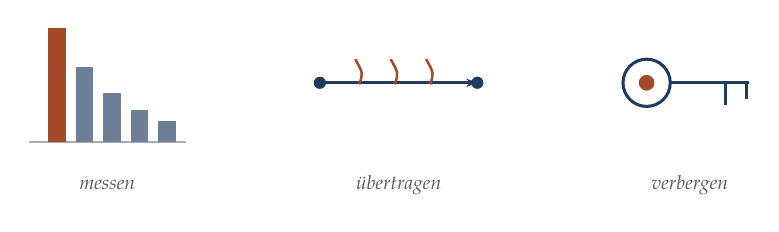
\begin{tikzpicture}[scale=1.0]
% messen: ungleiche Balken
\begin{scope}[xshift=-3.7cm]
\draw[grau!50, line width=0.6pt] (-1.0,-0.75) -- (1.0,-0.75);
\foreach \x/\h in {-0.75/1.45, -0.4/0.95, -0.05/0.62, 0.3/0.40, 0.65/0.26}
  \fill[tief!65] (\x,-0.75) rectangle ++(0.22,\h);
\fill[akzent] (-0.75,-0.75) rectangle ++(0.22,1.45);
\node[font=\scriptsize\itshape, color=grau] at (0,-1.3) {messen};
\end{scope}
% übertragen: Kanal mit Störung
\begin{scope}
\draw[tief, line width=1.0pt, -{Stealth[length=4pt]}] (-1.0,0.0) -- (1.0,0.0);
\foreach \x in {-0.55,-0.1,0.35}
  \draw[akzent, line width=0.9pt] (\x,0.30) .. controls (\x+0.1,0.12) .. (\x+0.05,-0.02);
\fill[tief] (-1.0,0.0) circle (2.2pt);
\fill[tief] (1.0,0.0) circle (2.2pt);
\node[font=\scriptsize\itshape, color=grau] at (0,-1.3) {übertragen};
\end{scope}
% verbergen: Schlüssel
\begin{scope}[xshift=3.7cm]
\draw[tief, line width=1.1pt] (-0.55,0.0) circle (0.30);
\draw[tief, line width=1.1pt] (-0.25,0.0) -- (0.75,0.0);
\draw[tief, line width=1.1pt] (0.45,0.0) -- (0.45,-0.28);
\draw[tief, line width=1.1pt] (0.72,0.0) -- (0.72,-0.20);
\fill[akzent] (-0.55,0.0) circle (0.10);
\node[font=\scriptsize\itshape, color=grau] at (0,-1.3) {verbergen};
\end{scope}
\end{tikzpicture}

\vspace{1.4cm}
{\large\color{grau} Von der Entropie bis zum Schlüsseltausch}\\[6pt]
{\color{grau} Jeder Schritt erklärt. Mit vollständig durchgerechneten Übungsaufgaben.}\\[1.9cm]
{\small\color{grau} Stand der Forschung: August 2026}
\end{titlepage}
\thispagestyle{empty}
\vspace*{\fill}
\begin{flushleft}
{\small\color{grau}
\textbf{\color{tief}Mathematik von Grund auf} --- Band 20\\[2pt]
\textit{Was Nachrichten wiegen} $\cdot$ Information und Kryptographie\\[14pt]

Herausgeber und Urheber: Jürgen Maier\\[2pt]
Entstanden 2026 in Zusammenarbeit mit Claude (Anthropic); Konzeption, Vorgaben, Prüfung und Herausgeberschaft: Jürgen Maier.\\[14pt]

\textbf{Lizenz}\\[2pt]
Dieses Werk ist lizenziert unter einer Creative-Commons-Lizenz \textbf{Namensnennung -- Weitergabe unter gleichen Bedingungen 4.0 International (CC BY-SA 4.0)}. Sie dürfen das Werk vervielfältigen, verbreiten, bearbeiten und auch kommerziell nutzen, sofern Sie den Urheber nennen und Bearbeitungen unter derselben Lizenz weitergeben.\\[2pt]
Lizenztext: \texttt{https://creativecommons.org/licenses/by-sa/4.0/legalcode.de}\\[14pt]

\textbf{Quellen und Fassungen}\\[2pt]
Quelltexte, Simulationen, Fehlermeldungen und aktuelle Fassungen aller Bände:\\
\texttt{https://github.com/juergenmaier2026/mathematik-von-grund-auf}\\[2pt]
Dauerhaft archiviert bei Zenodo: \texttt{https://doi.org/10.5281/zenodo.23698547}\\[14pt]

\textbf{Zitiervorschlag}\\[2pt]
Maier, J. (2026). \textit{Mathematik von Grund auf, Band 20: Was Nachrichten wiegen}. Fassung 1.0.1. \texttt{https://doi.org/10.5281/zenodo.23698547}\\[14pt]

Satz: \LaTeX{} mit Palatino. Fassung 1.0.1, Oktober 2026. 242 Seiten.
}
\end{flushleft}
\vspace*{1.5cm}

\tableofcontents
\mainmatter

\chapter*{Vorwort: Eine Größe, die niemand vermutet hatte}
\addcontentsline{toc}{chapter}{Vorwort}
\markboth{Vorwort}{Vorwort}

Bis 1948 war \enquote{Information} kein mathematischer Begriff. Danach war sie eine messbare Größe mit einer Einheit --- und mit Sätzen, die bis heute überraschen.

\begin{merksatz}
\boxtitel{Was dieser Band behauptet}
\begin{center}
\begin{minipage}{0.9\textwidth}
\textbf{Eine Nachricht hat ein Gewicht, das sich in Bit angeben lässt --- und dieses Gewicht hängt nicht davon ab, was sie bedeutet, sondern nur davon, wie überraschend sie ist.}
\end{minipage}
\end{center}

\begin{center}
\begin{minipage}{0.88\textwidth}
\kursiv{Das ist eine ungewöhnliche Behauptung, und sie hat einen Preis: Der Begriff sagt nichts über Bedeutung, Wahrheit oder Nutzen. Was er dafür leistet, sind Sätze von seltener Schärfe --- über Grenzen, die niemand unterbieten kann, und über Verfahren, die sie erreichen.}
\end{minipage}
\end{center}
\end{merksatz}

\section*{Drei Ergebnisse, die der Anschauung widersprechen}

\begin{merksatz}
\boxtitel{Was in diesem Band bewiesen wird}
\begin{center}
{\small
\renewcommand{\arraystretch}{1.55}
\begin{tabular}{@{}P{2.4cm}P{6.2cm}@{}}
\toprule
\textbf{Kapitel 3} & Es gibt eine Grenze, unter die keine Kompression kommen kann --- und Verfahren, die ihr beliebig nahe kommen.\\
\textbf{Kapitel 5} & Über einen \kursiv{gestörten} Kanal lässt sich mit beliebig kleiner Fehlerrate übertragen. Nicht langsamer, sondern nur bis zu einer festen Rate.\\
\textbf{Kapitel 9} & Es gibt eine Verschlüsselung, die beweisbar unbrechbar ist --- und einen Satz, der sagt, warum sie praktisch unbrauchbar bleibt.\\
\bottomrule
\end{tabular}}
\end{center}

\begin{center}
\begin{minipage}{0.9\textwidth}
Die mittlere Aussage ist die erstaunlichste. Vor 1948 hielt man es für selbstverständlich, dass Störungen die Fehlerrate erhöhen und man sie nur durch Wiederholung senken kann --- also durch Verlangsamung.
\end{minipage}
\end{center}

\begin{center}
\begin{minipage}{0.88\textwidth}
\kursiv{Shannon zeigte, dass das falsch ist. Es gibt eine feste Rate, die \Begriff{Kanalkapazität}, unterhalb derer die Fehlerrate beliebig klein gemacht werden kann, ohne die Rate weiter zu senken. Oberhalb davon geht es gar nicht. Der Übergang ist scharf.}
\end{minipage}
\end{center}
\end{merksatz}

\section*{Warum Kryptographie in denselben Band gehört}

\begin{merksatz}
\boxtitel{Derselbe Begriff, andere Richtung}
\begin{center}
{\small
\renewcommand{\arraystretch}{1.52}
\begin{tabular}{@{}P{2.4cm}P{2.8cm}P{2.8cm}@{}}
\toprule
& \textbf{Teil I--III} & \textbf{Teil IV--V}\\
\midrule
Ziel & Information erhalten & Information verbergen\\
Gegner & Rauschen & ein Mitleser\\
Maß & Entropie & Entropie\\
Grenze & Kapazität & Schlüssellänge\\
\bottomrule
\end{tabular}}
\end{center}

\begin{center}
\begin{minipage}{0.9\textwidth}
\textbf{Shannon hat beide Gebiete begründet --- 1948 die Informationstheorie, 1949 die mathematische Kryptographie.} Beide Arbeiten benutzen denselben Entropiebegriff.
\end{minipage}
\end{center}

\begin{center}
\begin{minipage}{0.88\textwidth}
\kursiv{Der Zusammenhang ist kein historischer Zufall. Perfekte Geheimhaltung bedeutet, dass der Geheimtext \kursiv{keine} Information über den Klartext enthält --- und das ist eine Aussage über Transinformation, also über genau die Größe aus Kapitel~4. Kapitel~9 beweist daraus, wie lang ein Schlüssel mindestens sein muss.}
\end{minipage}
\end{center}
\end{merksatz}

\section*{Was Sie mitbringen müssen}

\begin{merksatz}
\boxtitel{Die Voraussetzungen}
\begin{center}
{\small
\renewcommand{\arraystretch}{1.5}
\begin{tabular}{@{}P{3.0cm}P{5.6cm}@{}}
\toprule
\textbf{Logarithmen} & Rechenregeln, Basiswechsel. Schulmathematik.\\
\textbf{Wahrschein\-lichkeit} & Verteilungen, Erwartungswert, Unabhängigkeit, bedingte Wahrscheinlichkeit. Band 12.\\
\textbf{Konvexität} & Nur die Jensensche Ungleichung, ab Kapitel~2. Band 19, Kapitel~7.\\
\textbf{Modulare Arithmetik} & Erst ab Kapitel~11 --- und dort von Grund auf eingeführt. Band 8.\\
\textbf{Gruppen} & Erst ab Kapitel~12, ebenfalls dort erklärt. Band 6.\\
\bottomrule
\end{tabular}}
\end{center}

\begin{center}
\begin{minipage}{0.88\textwidth}
\kursiv{Die erste Hälfte kommt mit Wahrscheinlichkeitsrechnung aus. Die zweite braucht Zahlentheorie --- aber nur einen kleinen, genau umrissenen Teil davon, der in den Kapiteln~11 und 12 vollständig entwickelt wird. Man muss Band 8 nicht gelesen haben.}
\end{minipage}
\end{center}
\end{merksatz}

\section*{Das Klinikum Neustadt}

\begin{merksatz}
\boxtitel{Der Leitfall}
Wie in den Bänden 17 bis 19 läuft ein einziger erfundener Fall durch alle Kapitel --- diesmal die Digitalisierung eines Krankenhauses.

\begin{center}
{\small
\renewcommand{\arraystretch}{1.5}
\begin{tabular}{@{}P{1.6cm}P{2.6cm}P{3.8cm}@{}}
\toprule
\textbf{Teil} & \textbf{Thema} & \textbf{Der Leitfall zeigt}\\
\midrule
I & Messen & wie klein Befunddaten werden können\\
II & Übertragen & Funk zum Rettungswagen\\
III & Zufall & was ein Datensatz hergibt\\
IV & Geheimhalten & Patientendaten verschlüsseln\\
V & Öffentliche Schlüssel & Arztbriefe signieren\\
VI & Stand & was morgen noch sicher ist\\
\bottomrule
\end{tabular}}
\end{center}
\end{merksatz}

\section*{Drei Warnungen}

\begin{warnung}
\boxtitelr{Erstens: Information ist nicht Bedeutung}
Der Informationsgehalt einer Nachricht hängt allein von ihrer Wahrscheinlichkeit ab.

\begin{center}
\begin{minipage}{0.9\textwidth}
Eine zufällige Zeichenfolge hat mehr Information als ein Satz gleicher Länge --- weil sie unvorhersehbarer ist. Für die Übertragungstechnik ist das die richtige Größe. Für die Frage, was eine Nachricht \kursiv{wert} ist, taugt sie nicht.
\end{minipage}
\end{center}
\end{warnung}

\begin{warnung}
\boxtitelr{Zweitens: Sätze gelten für Grenzwerte}
Shannons Ergebnisse sind Aussagen über beliebig lange Nachrichten.

\begin{center}
\begin{minipage}{0.88\textwidth}
\kursiv{\enquote{Beliebig kleine Fehlerrate} heißt: für hinreichend große Blocklänge. Wie groß, sagt der Satz nicht --- und für praktische Blocklängen kann die Lücke erheblich sein. Kapitel~6 behandelt, was tatsächlich erreichbar ist.}
\end{minipage}
\end{center}
\end{warnung}

\begin{warnung}
\boxtitelr{Drittens: Sicherheit ist nicht beweisbar}
Mit einer einzigen Ausnahme --- dem Einmalschlüssel aus Kapitel~9 --- beruht jedes praktisch verwendete Verfahren auf einer \kursiv{Annahme}.

\begin{center}
\begin{minipage}{0.9\textwidth}
\textbf{Man nimmt an, dass ein bestimmtes Rechenproblem schwer ist. Bewiesen ist das bei keinem einzigen.}
\end{minipage}
\end{center}

\begin{center}
\begin{minipage}{0.88\textwidth}
\kursiv{Das ist derselbe Stand wie bei $\mathsf{P}$ gegen $\mathsf{NP}$ in Band 19, Kapitel~12 --- und hängt unmittelbar damit zusammen. Wäre $\mathsf{P}=\mathsf{NP}$, so wäre nahezu die gesamte heutige Kryptographie hinfällig. \textbf{Die Sicherheit der digitalen Welt ruht auf einer unbewiesenen Vermutung}, und dieser Band sagt das an jeder Stelle, an der es zutrifft.}
\end{minipage}
\end{center}
\end{warnung}

\section*{Der Aufbau}

\begin{merksatz}
\boxtitel{Sechs Teile, fünfzehn Kapitel}
\begin{center}
{\small
\renewcommand{\arraystretch}{1.45}
\begin{tabular}{@{}P{1.0cm}P{3.2cm}P{4.4cm}@{}}
\toprule
\textbf{Teil} & \textbf{Thema} & \textbf{Die Leitfrage}\\
\midrule
I & Information messen (1--3) & Wie klein geht es?\\
II & Der gestörte Kanal (4--6) & Wie schnell geht es fehlerfrei?\\
III & Zufall (7--8) & Was heißt zufällig?\\
IV & Geheimhaltung (9--11) & Was ist beweisbar sicher?\\
V & Öffentliche Schlüssel (12--14) & Wie tauscht man Schlüssel ohne Kanal?\\
VI & Stand (15) & Was hält dem Quantenrechner stand?\\
\bottomrule
\end{tabular}}
\end{center}
\end{merksatz}

\vspace{10pt}
\begin{flushright}
\itshape\color{grau}
Information ist die Auflösung\\
von Ungewissheit.\\[8pt]
\normalfont\color{grau}\upshape --- nach Claude Shannon, 1948
\end{flushright}

\part{Information messen}

\chapter{Was Information ist}

\section{Der Leitfall}

\begin{merksatz}
\boxtitel{Das Klinikum Neustadt wird digital}
Jeder Behandlungsfall erhält einen Diagnoseschlüssel aus acht Gruppen. Die Häufigkeiten über ein Jahr:

\begin{center}
{\small
\renewcommand{\arraystretch}{1.48}
\begin{tabular}{@{}P{1.6cm}P{1.8cm}P{1.6cm}P{1.8cm}@{}}
\toprule
\textbf{Gruppe} & \textbf{Anteil} & \textbf{Gruppe} & \textbf{Anteil}\\
\midrule
$A$ & $0{,}2500$ & $E$ & $0{,}0625$\\
$B$ & $0{,}2500$ & $F$ & $0{,}0625$\\
$C$ & $0{,}1250$ & $G$ & $0{,}0625$\\
$D$ & $0{,}1250$ & $H$ & $0{,}0625$\\
\bottomrule
\end{tabular}}
\end{center}

\schritt{Die naheliegende Codierung}
Acht Gruppen, also drei Bit je Fall: $000$ für $A$, $001$ für $B$ und so fort.

\textbf{Die Frage:} Geht es kürzer?

\begin{center}
\begin{minipage}{0.88\textwidth}
\kursiv{Die Antwort lautet ja --- und zwar auf $2{,}75$ Bit im Mittel, nicht weniger. Beide Teile dieser Aussage sind Sätze: dass es geht, und dass es nicht besser geht. Kapitel~3 beweist sie. Zuvor muss geklärt werden, woher die Zahl $2{,}75$ kommt.}
\end{minipage}
\end{center}
\end{merksatz}

\section{Was Information nicht ist}

\begin{warnung}
\boxtitelr{Drei Verwechslungen}
\begin{center}
{\small
\renewcommand{\arraystretch}{1.52}
\begin{tabular}{@{}P{2.4cm}P{6.2cm}@{}}
\toprule
\textbf{Bedeutung} & \enquote{Der Patient lebt} und \enquote{der Patient ist verstorben} können denselben Informationsgehalt haben. Der Begriff misst nicht, was es bedeutet.\\
\textbf{Wahrheit} & Eine falsche Nachricht hat denselben Gehalt wie eine richtige gleicher Wahrscheinlichkeit.\\
\textbf{Nutzen} & Eine unwahrscheinliche und völlig belanglose Nachricht hat viel Information.\\
\bottomrule
\end{tabular}}
\end{center}

\begin{center}
\begin{minipage}{0.9\textwidth}
\textbf{Der Informationsgehalt misst allein, wie sehr eine Nachricht die Ungewissheit des Empfängers auflöst.}
\end{minipage}
\end{center}

\begin{center}
\begin{minipage}{0.88\textwidth}
\kursiv{Shannon hat das ausdrücklich betont: Die Bedeutungsfrage sei für das technische Problem \kursiv{unerheblich}. Das wurde ihm oft als Mangel ausgelegt und ist der Grund für den Erfolg der Theorie --- eine Größe, die von der Bedeutung absieht, gilt für jede Art von Nachricht gleichermaßen.}
\end{minipage}
\end{center}
\end{warnung}

\section{Der Informationsgehalt eines Ereignisses}

\begin{merksatz}
\boxtitel{Drei Forderungen}
Wir suchen eine Funktion $I(p)$, die den Gehalt eines Ereignisses der Wahrscheinlichkeit $p$ angibt.

\begin{center}
{\small
\renewcommand{\arraystretch}{1.55}
\begin{tabular}{@{}P{1.0cm}P{7.4cm}@{}}
\toprule
$1$ & $I$ hängt nur von $p$ ab und ist stetig.\\
$2$ & $I$ ist monoton fallend: Seltenes überrascht mehr.\\
$3$ & Für unabhängige Ereignisse addieren sich die Gehalte:\\
& \qquad $I(p\cdot q) = I(p) + I(q)$\\
\bottomrule
\end{tabular}}
\end{center}

\schritt{Warum die dritte Forderung}
Erfährt man zwei unabhängige Dinge, so soll die Gesamtinformation die Summe sein. Die Wahrscheinlichkeit des gemeinsamen Ereignisses ist das \kursiv{Produkt}.

\begin{center}
\begin{minipage}{0.9\textwidth}
\textbf{Gesucht ist also eine Funktion, die Produkte in Summen verwandelt.} Damit ist die Antwort im Grunde schon gegeben.
\end{minipage}
\end{center}
\end{merksatz}

\begin{merksatz}
\boxtitel{Satz 1.1 --- die Forderungen legen $I$ fest}
Erfüllt $I:(0,1] \to \R$ die drei Forderungen, so gibt es eine Konstante $C > 0$ mit
\[ I(p) = -C\,\ln p . \]

\schritt{Beweis --- Schritt 1: die Substitution}
Wir setzen $p = e^{-x}$ mit $x \ge 0$ und definieren
\[ g(x) := I(e^{-x}) . \]
Da $p \mapsto -\ln p$ stetig und streng fallend ist, ist $g$ stetig.

\schritt{Schritt 2 --- die Funktionalgleichung}
Aus $I(pq) = I(p)+I(q)$ mit $p = e^{-x}$ und $q = e^{-y}$, also $pq = e^{-(x+y)}$:
\[ g(x+y) = g(x) + g(y) \qquad\text{für alle } x,y \ge 0 . \]

\schritt{Schritt 3 --- ganzzahlige Vielfache}
Setzt man $y = x$, so folgt $g(2x) = 2g(x)$; durch Wiederholung
\[ g(nx) = n\,g(x) \qquad\text{für alle } n \in \mathbb{N} . \]

Mit $x = \frac{1}{n}$ und $c := g(1)$:
\[ c = g(1) = g\left(n\cdot\tfrac1n\right) = n\,g\left(\tfrac1n\right) \quad\Longrightarrow\quad g\left(\tfrac1n\right) = \tfrac{c}{n} \]

\schritt{Schritt 4 --- rationale Zahlen}
Für $x = \frac{m}{n}$:
\[ g\left(\tfrac{m}{n}\right) = m\,g\left(\tfrac1n\right) = \tfrac{m}{n}\,c \]

\schritt{Schritt 5 --- alle reellen Zahlen}
Die Funktion $g$ ist stetig und stimmt auf den rationalen Zahlen mit $x \mapsto cx$ überein. Da die rationalen Zahlen dicht liegen, gilt
\[ g(x) = c\,x \qquad\text{für alle } x \ge 0 . \]

\schritt{Schritt 6 --- zurückübersetzen}
Mit $x = -\ln p$:
\[ I(p) = g(-\ln p) = -c\,\ln p \]

Aus Forderung 2 folgt $c > 0$: Für kleineres $p$ ist $-\ln p$ größer, und $I$ soll dann größer sein. $\blacksquare$

\begin{center}
\begin{minipage}{0.88\textwidth}
\kursiv{Bemerkenswert ist, wie wenig gefordert wurde. Drei sehr schwache Bedingungen --- Stetigkeit, Monotonie, Additivität bei Unabhängigkeit --- legen die Funktion bis auf einen Faktor \kursiv{vollständig} fest. Der Faktor bestimmt nur die Maßeinheit.}
\end{minipage}
\end{center}
\end{merksatz}

\begin{definition}
\boxtitelm{Definition 1.2 --- das Bit}
Wählt man $C = \frac{1}{\ln 2}$, so wird
\[ I(p) = -\lb p = \lb\frac1p \]
mit dem Logarithmus zur Basis $2$. Die Einheit heißt \Begriff{Bit}.
\end{definition}

\begin{merksatz}
\boxtitel{Warum die Basis zwei}
\begin{center}
\begin{minipage}{0.9\textwidth}
\textbf{Ein Ereignis der Wahrscheinlichkeit $\frac12$ hat genau ein Bit Information.}
\end{minipage}
\end{center}

\[ I\left(\tfrac12\right) = \lb 2 = 1 \]

Das entspricht einer Ja-Nein-Frage: Der Ausgang eines fairen Münzwurfs ist genau ein Bit.

\schritt{Die Werte im Leitfall}
\begin{center}
{\small
\renewcommand{\arraystretch}{1.48}
\begin{tabular}{@{}P{1.8cm}P{1.8cm}P{2.2cm}P{2.0cm}@{}}
\toprule
\textbf{Gruppe} & $p$ & $1/p$ & $I = \lb(1/p)$\\
\midrule
$A$, $B$ & $0{,}2500$ & $4$ & $2$ Bit\\
$C$, $D$ & $0{,}1250$ & $8$ & $3$ Bit\\
$E$--$H$ & $0{,}0625$ & $16$ & $4$ Bit\\
\bottomrule
\end{tabular}}
\end{center}

\begin{center}
\begin{minipage}{0.9\textwidth}
\textbf{Die häufigen Gruppen tragen zwei Bit, die seltenen vier.} Genau darauf beruht die Ersparnis: Man gibt den häufigen Fällen kurze Codewörter.
\end{minipage}
\end{center}

\schritt{Andere Einheiten}
\begin{center}
\renewcommand{\arraystretch}{1.5}
\begin{tabular}{@{}P{2.0cm}P{2.4cm}P{3.0cm}@{}}
\toprule
\textbf{Basis} & \textbf{Einheit} & \textbf{Umrechnung}\\
\midrule
$2$ & Bit & ---\\
$e$ & Nat & $1$ Nat $= 1{,}443$ Bit\\
$10$ & Hartley & $1$ Hartley $= 3{,}322$ Bit\\
\bottomrule
\end{tabular}
\end{center}

\begin{center}
\begin{minipage}{0.88\textwidth}
\kursiv{Die Umrechnung ist ein reiner Basiswechsel: $\lb x = \frac{\ln x}{\ln 2}$, und $\frac{1}{\ln 2} = 1{,}4427$. In der Theorie rechnet man oft mit Nat, weil die Ableitungen einfacher werden; in der Technik stets mit Bit.}
\end{minipage}
\end{center}
\end{merksatz}

\section{Die Eigenschaften}

\begin{merksatz}
\boxtitel{Was die Formel leistet}
\begin{center}
{\small
\renewcommand{\arraystretch}{1.5}
\begin{tabular}{@{}P{2.4cm}P{2.6cm}P{3.0cm}@{}}
\toprule
$p$ & $I(p)$ & \textbf{Deutung}\\
\midrule
$1$ & $0$ & Sicheres trägt nichts bei\\
$0{,}5$ & $1$ Bit & Münzwurf\\
$0{,}01$ & $6{,}64$ Bit & seltenes Ereignis\\
$10^{-6}$ & $19{,}93$ Bit & sehr seltenes\\
$\to 0$ & $\to\infty$ & unbeschränkt\\
\bottomrule
\end{tabular}}
\end{center}

\schritt{Die erste Zeile}
\[ I(1) = \lb 1 = 0 \]

\begin{center}
\begin{minipage}{0.9\textwidth}
\textbf{Die Mitteilung eines sicheren Ereignisses trägt null Bit.} Wer sagt, dass die Sonne aufgegangen ist, teilt nichts mit.
\end{minipage}
\end{center}

\schritt{Die letzte Zeile}
Je unwahrscheinlicher, desto mehr Information --- ohne obere Grenze.

\begin{center}
\begin{minipage}{0.88\textwidth}
\kursiv{Das Wachstum ist allerdings langsam: Eine millionenfach kleinere Wahrscheinlichkeit bringt nur den Faktor $20$ statt $6{,}64$, also gut das Dreifache. Der Logarithmus dämpft stark --- und genau das macht die Größe handhabbar.}
\end{minipage}
\end{center}
\end{merksatz}

\begin{merksatz}
\boxtitel{Die Additivität nachgerechnet}
Zwei unabhängige Befunde: Gruppe $A$ ($p=0{,}25$) und ein positiver Laborwert ($p=0{,}125$).

\begin{center}
\renewcommand{\arraystretch}{1.5}
\begin{tabular}{@{}P{2.8cm}P{2.4cm}P{2.4cm}@{}}
\toprule
\textbf{Ereignis} & $p$ & $I$\\
\midrule
Gruppe $A$ & $0{,}2500$ & $2$ Bit\\
Labor positiv & $0{,}1250$ & $3$ Bit\\
\midrule
beides & $0{,}03125$ & $\mathbf{5}$ Bit\\
\bottomrule
\end{tabular}
\end{center}

\kursiv{Probe:} $0{,}25 \cdot 0{,}125 = 0{,}03125 = \frac{1}{32}$, und $\lb 32 = 5$. \checkmark

\begin{center}
\begin{minipage}{0.88\textwidth}
\kursiv{Die Additivität ist keine Eigenschaft, die man beobachtet hätte --- sie war die \kursiv{Forderung}, aus der die Formel folgte. Das ist die übliche Reihenfolge in der Informationstheorie: Man schreibt auf, was eine Größe leisten soll, und findet, dass es nur eine gibt.}
\end{minipage}
\end{center}
\end{merksatz}

\section{Der Bruchfall}

\begin{warnung}
\boxtitelr{Was vorausgesetzt wird}
\begin{center}
{\small
\renewcommand{\arraystretch}{1.52}
\begin{tabular}{@{}P{2.8cm}P{5.8cm}@{}}
\toprule
\textbf{Die Verteilung} & $I(p)$ setzt voraus, dass $p$ bekannt ist. In der Praxis wird sie geschätzt --- mit allen Schwierigkeiten aus Band 17.\\
\textbf{Unabhängigkeit} & Forderung 3 gilt nur dort. Bei abhängigen Ereignissen ist die Summe der Einzelgehalte zu groß.\\
\textbf{Ein Empfänger} & Der Gehalt hängt davon ab, was der Empfänger schon weiß. Für verschiedene Empfänger ist er verschieden.\\
\bottomrule
\end{tabular}}
\end{center}

\schritt{Zur zweiten Zeile}
Diagnosegruppe und Laborwert sind in Wirklichkeit nicht unabhängig. Gilt etwa
\[ \Pr[\text{Labor}\mid A] = 0{,}5 \quad\text{statt}\quad 0{,}125 , \]
so ist der gemeinsame Gehalt
\[ I(0{,}25 \cdot 0{,}5) = I(0{,}125) = 3 \ \text{Bit} \]
statt fünf.

\begin{center}
\begin{minipage}{0.9\textwidth}
\textbf{Zwei Bit sind verschwunden --- sie waren doppelt gezählt.} Diese Größe hat einen Namen: Sie ist die Transinformation zwischen Gruppe und Laborwert.
\end{minipage}
\end{center}

\begin{center}
\begin{minipage}{0.88\textwidth}
\kursiv{Damit ist der Begriff eingeführt, der Teil~II trägt. \textbf{Abhängigkeit bedeutet, dass eine Größe etwas über die andere verrät} --- und die Transinformation misst, wie viel. Kapitel~4 macht daraus eine Definition.}
\end{minipage}
\end{center}

\schritt{Zur dritten Zeile}
\begin{center}
\begin{minipage}{0.88\textwidth}
\kursiv{Der Informationsgehalt ist keine Eigenschaft der Nachricht, sondern der Beziehung zwischen Nachricht und Empfänger. Wer die Diagnose bereits kennt, erfährt null Bit. Das klingt nach einem Mangel und ist die richtige Modellierung: Information ist Auflösung von Ungewissheit, und Ungewissheit hat jemand.}
\end{minipage}
\end{center}
\end{warnung}

\begin{warnung}
\boxtitelr{Und eine begriffliche Falle}
Das Wort \enquote{Bit} bezeichnet zweierlei:

\begin{center}
{\small
\renewcommand{\arraystretch}{1.5}
\begin{tabular}{@{}P{2.4cm}P{6.2cm}@{}}
\toprule
\textbf{Als Einheit} & Ein Maß für Information --- kann jeden nichtnegativen reellen Wert annehmen, etwa $2{,}75$.\\
\textbf{Als Zeichen} & Eine Binärstelle, also $0$ oder $1$. Davon gibt es immer ganze Zahlen.\\
\bottomrule
\end{tabular}}
\end{center}

\begin{center}
\begin{minipage}{0.9\textwidth}
\textbf{Der ganze Teil~I handelt vom Abstand zwischen beidem:} Wie viele Binärstellen braucht man, um eine Information von $2{,}75$ Bit zu übertragen?
\end{minipage}
\end{center}

\begin{center}
\begin{minipage}{0.88\textwidth}
\kursiv{Die Antwort ist nicht drei, sondern --- im Mittel über viele Fälle --- genau $2{,}75$. Dass ein nicht ganzzahliger Wert erreichbar ist, obwohl jede einzelne Nachricht aus ganzen Binärstellen besteht, ist das erste überraschende Ergebnis dieses Bandes. Kapitel~3 zeigt, wie.}
\end{minipage}
\end{center}
\end{warnung}

\section{Übungsaufgaben}

\begin{aufgabe}
\boxtitel{Aufgabe 1.1 --- Informationsgehalte bestimmen}
Berechnen Sie den Informationsgehalt in Bit:
\begin{center}
{\small
\renewcommand{\arraystretch}{1.4}
\begin{tabular}{@{}P{0.8cm}P{7.6cm}@{}}
\toprule
(a) & Ein Würfel zeigt eine Sechs.\\
(b) & Ein Würfel zeigt eine gerade Zahl.\\
(c) & Zwei Würfel zeigen zusammen zwölf.\\
(d) & Eine zufällige Ziffernfolge der Länge $6$.\\
(e) & Ein Patient gehört zur Gruppe $E$ (Anteil $0{,}0625$).\\
\bottomrule
\end{tabular}}
\end{center}

\loesung
\schritt{(a)}
\[ p = \tfrac16, \qquad I = \lb 6 = \frac{\ln 6}{\ln 2} = \frac{1{,}7918}{0{,}6931} = 2{,}585 \ \text{Bit} \]

\schritt{(b)}
\[ p = \tfrac12, \qquad I = 1 \ \text{Bit} \]

\schritt{(c)}
Beide müssen Sechsen zeigen:
\[ p = \tfrac16\cdot\tfrac16 = \tfrac1{36}, \qquad I = \lb 36 = 5{,}170 \ \text{Bit} \]

\kursiv{Probe über die Additivität:} $2\cdot2{,}585 = 5{,}170$ \checkmark

\schritt{(d)}
Jede der zehn Ziffern ist gleich wahrscheinlich, die Stellen sind unabhängig:
\[ p = 10^{-6}, \qquad I = 6\,\lb 10 = 6\cdot3{,}3219 = 19{,}93 \ \text{Bit} \]

\begin{center}
\begin{minipage}{0.86\textwidth}
\kursiv{Zwanzig Bit für sechs Ziffern --- das sind $3{,}32$ Bit je Ziffer. Speichert man jede Ziffer in vier Binärstellen, so verschenkt man $0{,}68$ Bit je Ziffer, also gut siebzehn Prozent. Genau diese Art von Verschwendung behebt Kapitel~3.}
\end{minipage}
\end{center}

\schritt{(e)}
\[ p = 0{,}0625 = \tfrac1{16}, \qquad I = \lb 16 = 4 \ \text{Bit} \]

\schritt{Die Übersicht}
\begin{center}
\renewcommand{\arraystretch}{1.46}
\begin{tabular}{@{}P{1.0cm}P{2.2cm}P{2.4cm}@{}}
\toprule
& $p$ & $I$ in Bit\\
\midrule
(a) & $0{,}1667$ & $2{,}585$\\
(b) & $0{,}5000$ & $1{,}000$\\
(c) & $0{,}0278$ & $5{,}170$\\
(d) & $10^{-6}$ & $19{,}93$\\
(e) & $0{,}0625$ & $4{,}000$\\
\bottomrule
\end{tabular}
\end{center}

\begin{center}
\begin{minipage}{0.86\textwidth}
\kursiv{Bemerkenswert ist (d) im Vergleich zu (c): Eine millionenfach kleinere Wahrscheinlichkeit bringt nur den vierfachen Informationsgehalt. Der Logarithmus dämpft so stark, dass auch extrem seltene Ereignisse handhabbare Zahlen liefern.}
\end{minipage}
\end{center}
\end{aufgabe}

\begin{aufgabe}
\boxtitel{Aufgabe 1.2 --- Warum nur der Logarithmus}
Prüfen Sie, welche der drei Forderungen die folgenden Funktionen verletzen.
\begin{center}
{\small
\renewcommand{\arraystretch}{1.4}
\begin{tabular}{@{}P{0.8cm}P{7.6cm}@{}}
\toprule
(a) & $I(p) = 1-p$\\
(b) & $I(p) = \frac1p - 1$\\
(c) & $I(p) = -\lb p$ für $p \ge \frac12$, sonst $2$\\
(d) & $I(p) = (-\ln p)^2$\\
\bottomrule
\end{tabular}}
\end{center}

\loesung
\schritt{(a) $I(p)=1-p$}
\kursiv{Forderung 1:} stetig \checkmark\\
\kursiv{Forderung 2:} fallend \checkmark\\
\kursiv{Forderung 3:} Zu prüfen ist $I(pq) = I(p)+I(q)$:
\[ 1-pq \stackrel{?}{=} (1-p)+(1-q) = 2-p-q \]
Für $p=q=\tfrac12$: links $1-\tfrac14 = 0{,}75$, rechts $2-1 = 1$.

\textcolor{akzent}{Forderung 3 verletzt.}

\schritt{(b) $I(p) = \frac1p-1$}
\kursiv{Forderungen 1 und 2:} erfüllt.\\
\kursiv{Forderung 3:}
\[ \frac{1}{pq}-1 \stackrel{?}{=} \frac1p+\frac1q-2 \]
Für $p=q=\tfrac12$: links $4-1 = 3$, rechts $2+2-2 = 2$.

\textcolor{akzent}{Verletzt.}

\begin{center}
\begin{minipage}{0.86\textwidth}
\kursiv{Interessant ist, \kursiv{wie} es verletzt wird: Der Gehalt wächst zu schnell. Bei $p = 10^{-6}$ lieferte diese Formel den Wert $999\,999$ statt $19{,}93$. Ein solches Maß wäre von den seltenen Ereignissen beherrscht --- dieselbe Schwierigkeit wie bei der Varianz in Band 17.}
\end{minipage}
\end{center}

\schritt{(c) Die abschnittsweise Funktion}
Bei $p = \tfrac12$ ist $-\lb\tfrac12 = 1$; für $p$ knapp unter $\tfrac12$ springt der Wert auf $2$.

\textcolor{akzent}{Forderung 1 verletzt} --- nicht stetig.

\kursiv{Forderung 2} ist erfüllt (die Funktion fällt), \kursiv{Forderung 3} nicht.

\begin{center}
\begin{minipage}{0.86\textwidth}
\kursiv{Dieses Beispiel zeigt, dass die Stetigkeit im Beweis von Satz 1.1 wirklich gebraucht wird: Ohne sie gibt es tatsächlich weitere Lösungen der Funktionalgleichung --- allerdings sehr unangenehme, die sich nicht durch eine Formel hinschreiben lassen. Man nennt sie Hamel-Funktionen; ihre Existenz folgt aus dem Auswahlaxiom.}
\end{minipage}
\end{center}

\schritt{(d) $I(p) = (-\ln p)^2$}
\kursiv{Forderungen 1 und 2:} erfüllt.\\
\kursiv{Forderung 3:} Mit $u = -\ln p$, $v = -\ln q$ ist $-\ln(pq) = u+v$:
\[ (u+v)^2 = u^2 + 2uv + v^2 \ \ne\ u^2+v^2 \quad\text{für } u,v > 0 \]

\textcolor{akzent}{Verletzt --- um den Term $2uv$.}

\schritt{Die Bilanz}
\begin{center}
{\small
\renewcommand{\arraystretch}{1.46}
\begin{tabular}{@{}P{1.0cm}P{1.6cm}P{1.6cm}P{1.6cm}@{}}
\toprule
& \textbf{stetig} & \textbf{fallend} & \textbf{additiv}\\
\midrule
(a) & \checkmark & \checkmark & \textcolor{akzent}{nein}\\
(b) & \checkmark & \checkmark & \textcolor{akzent}{nein}\\
(c) & \textcolor{akzent}{nein} & \checkmark & \textcolor{akzent}{nein}\\
(d) & \checkmark & \checkmark & \textcolor{akzent}{nein}\\
\bottomrule
\end{tabular}}
\end{center}

\begin{center}
\begin{minipage}{0.88\textwidth}
\kursiv{Alle vier scheitern an der Additivität --- und das ist kein Zufall, sondern Satz 1.1: \textbf{Sie ist die eigentlich einschränkende Forderung.} Stetigkeit und Monotonie erfüllen unendlich viele Funktionen; die Additivität lässt nur eine übrig.}
\end{minipage}
\end{center}
\end{aufgabe}

\begin{aufgabe}
\boxtitel{Aufgabe 1.3 --- Das Wägeproblem}
Unter zwölf gleich aussehenden Münzen ist eine gefälscht --- sie ist entweder leichter oder schwerer. Wie viele Wägungen mit einer Balkenwaage braucht man mindestens, um sie zu finden \kursiv{und} zu sagen, ob sie zu leicht oder zu schwer ist?

\loesung
\schritt{Schritt 1 --- Die zu gewinnende Information}
Es gibt $12 \cdot 2 = 24$ mögliche Antworten, alle gleich wahrscheinlich:
\[ I = \lb 24 = \frac{\ln 24}{\ln 2} = \frac{3{,}1781}{0{,}6931} = 4{,}585 \ \text{Bit} \]

\schritt{Schritt 2 --- Die Information je Wägung}
Eine Balkenwaage hat drei mögliche Ausgänge: links schwerer, rechts schwerer, Gleichgewicht.

\begin{center}
\begin{minipage}{0.9\textwidth}
\textbf{Höchstens} $\lb 3 = 1{,}585$ Bit je Wägung --- und zwar genau dann, wenn alle drei Ausgänge gleich wahrscheinlich sind.
\end{minipage}
\end{center}

\schritt{Schritt 3 --- Die untere Schranke}
\[ n \cdot 1{,}585 \ \ge\ 4{,}585 \quad\Longrightarrow\quad n \ge 2{,}89 \]

Da $n$ ganzzahlig ist: $n \ge 3$.

\schritt{Schritt 4 --- Die Probe}
\[ 3^3 = 27 \ \ge\ 24 \quad \checkmark \]
\[ 3^2 = 9 \ < \ 24 \quad \text{--- zwei Wägungen reichen nicht.} \]

\schritt{Schritt 5 --- Dass drei genügen}
\kursiv{Erste Wägung:} Vier gegen vier.

\begin{center}
{\small
\renewcommand{\arraystretch}{1.5}
\begin{tabular}{@{}P{2.4cm}P{2.4cm}P{3.0cm}@{}}
\toprule
\textbf{Ausgang} & \textbf{Verdächtige} & \textbf{Rest}\\
\midrule
Gleichgewicht & die übrigen $4$ & $8$ Fälle\\
links schwerer & diese $8$ & $8$ Fälle\\
rechts schwerer & diese $8$ & $8$ Fälle\\
\bottomrule
\end{tabular}}
\end{center}

In jedem Fall bleiben acht Möglichkeiten. Mit zwei weiteren Wägungen sind $3^2 = 9 \ge 8$ unterscheidbar --- es geht.

\begin{center}
\begin{minipage}{0.88\textwidth}
\kursiv{Die Durchführung der beiden Restwägungen ist eine hübsche Knobelei und steht in jedem Rätselbuch. Der Punkt hier ist ein anderer: \textbf{Die Informationstheorie liefert die untere Schranke, ohne dass man das Verfahren kennt.} Sie sagt \enquote{weniger als drei geht nicht} --- und zwar bevor irgendjemand eine Wägestrategie erdacht hat.}
\end{minipage}
\end{center}

\schritt{Schritt 6 --- Die Verallgemeinerung}
Bei $m$ Münzen sind $2m$ Antworten zu unterscheiden, also
\[ n \ \ge\ \frac{\lb(2m)}{\lb 3} = \log_3(2m) . \]

\begin{center}
\renewcommand{\arraystretch}{1.46}
\begin{tabular}{@{}P{1.8cm}P{2.0cm}P{2.4cm}@{}}
\toprule
$m$ & $2m$ & \textbf{Schranke}\\
\midrule
$4$ & $8$ & $2$\\
$12$ & $24$ & $3$\\
$13$ & $26$ & $3$\\
$14$ & $28$ & $\mathbf{4}$\\
$39$ & $78$ & $4$\\
\bottomrule
\end{tabular}
\end{center}

\begin{center}
\begin{minipage}{0.86\textwidth}
\kursiv{Bei dreizehn Münzen sagt die Schranke drei, und tatsächlich genügen drei nicht ganz --- man kann die Fälschung finden, aber nicht immer sagen, ob sie leichter oder schwerer ist. \textbf{Eine informationstheoretische Schranke ist notwendig, nicht hinreichend.} Sie schließt aus, sie garantiert nicht. Derselbe Vorbehalt gilt für alle Sätze dieses Bandes.}
\end{minipage}
\end{center}
\end{aufgabe}

\begin{geschichte}
\boxtitelg{Eine Arbeit von 1948}
\Person{Claude Shannon} (1916--2001) veröffentlichte im Juli und Oktober 1948 in zwei Teilen die Arbeit \kursiv{A Mathematical Theory of Communication}. Sie umfasst gut fünfzig Seiten und begründete ein Fach.

\begin{center}
\begin{minipage}{0.9\textwidth}
\kursiv{Bemerkenswert ist die Geschlossenheit: Die Arbeit enthält den Entropiebegriff, den Quellencodierungssatz, die Kanalkapazität, das Kanalcodierungstheorem und die Erweiterung auf stetige Signale --- alles auf einmal, alles neu, und alles im Wesentlichen in der bis heute gültigen Form.}
\end{minipage}
\end{center}

\schritt{Die Vorläufer}
\Person{Harry Nyquist} (1924) und \Person{Ralph Hartley} (1928) hatten bei denselben Bell-Laboratorien vorgearbeitet. Hartley schlug vor, den Informationsgehalt einer Nachricht aus $n$ Zeichen über einem Alphabet der Größe $s$ als $n\log s$ zu messen.

\begin{center}
\begin{minipage}{0.9\textwidth}
\kursiv{Das ist der Sonderfall gleicher Wahrscheinlichkeiten: Bei $s$ gleich wahrscheinlichen Zeichen ist jedes $\lb s$ Bit wert. Hartley fehlte der Schritt zu ungleichen Wahrscheinlichkeiten --- und damit der ganze Rest. Die Einheit Hartley trägt seinen Namen.}
\end{minipage}
\end{center}

\schritt{Der Name}
Shannon berichtete, \Person{John von Neumann} habe ihm den Namen \enquote{Entropie} empfohlen --- mit der Begründung, die Funktion sei in der statistischen Mechanik unter diesem Namen bereits bekannt, und im Übrigen wisse ohnehin niemand, was Entropie sei, was ihm in Diskussionen stets einen Vorteil verschaffen werde.

\begin{center}
\begin{minipage}{0.9\textwidth}
\kursiv{Die Anekdote ist vielfach überliefert und in ihren Einzelheiten unsicher. Der sachliche Kern stimmt aber: Die Formel $-\sum p_i\ln p_i$ stand seit \Person{Boltzmann} und \Person{Gibbs} in der Physik, und der Zusammenhang ist mehr als eine Ähnlichkeit --- Kapitel~2 kommt darauf zurück.}
\end{minipage}
\end{center}

\schritt{Shannon selbst}
Er arbeitete bis 1972 an den Bell-Laboratorien und lehrte am MIT. Seine Dissertation von 1937 --- über die Anwendung der Booleschen Algebra auf Schaltkreise --- gilt als eine der folgenreichsten überhaupt.

\begin{center}
\begin{minipage}{0.9\textwidth}
\kursiv{Shannon war für seine Zurückhaltung und seine Bastelfreude bekannt; er baute unter anderem eine jonglierende Maschine und ein Einrad mit außermittigem Sattel. Auf die Frage, warum er nach 1948 kaum noch zur Informationstheorie veröffentlichte, antwortete er sinngemäß, das Wesentliche sei gesagt.}
\end{minipage}
\end{center}
\end{geschichte}

\begin{forschung}
\boxtitelp{Wo der Begriff heute steckt}
\begin{center}
{\small
\renewcommand{\arraystretch}{1.45}
\begin{tabular}{@{}P{2.8cm}P{5.4cm}@{}}
\toprule
\textbf{Technik} & Jede Datenübertragung und jede Kompression beruht auf den Sätzen dieses Bandes.\\
\textbf{Statistik} & Modellwahl über Informationskriterien; die Kullback-Leibler-Divergenz aus Kapitel~8.\\
\textbf{Physik} & Die Verbindung zur thermodynamischen Entropie; das Landauer-Prinzip.\\
\textbf{Biologie} & Informationsgehalt von Sequenzen, Kanalmodelle für die Signalübertragung in Zellen.\\
\bottomrule
\end{tabular}}
\end{center}

\schritt{Zur dritten Zeile}
\Person{Rolf Landauer} zeigte 1961, dass das \kursiv{Löschen} eines Bits mindestens die Wärmemenge $k_B T \ln 2$ freisetzen muss.

\begin{center}
\begin{minipage}{0.88\textwidth}
\kursiv{Bei Raumtemperatur sind das etwa $3 \cdot 10^{-21}$ Joule --- verschwindend wenig gegenüber dem tatsächlichen Energieverbrauch heutiger Rechner, aber grundsätzlich. Die Aussage wurde 2012 erstmals experimentell bestätigt. Sie besagt, dass Information keine rein mathematische Größe ist: Ihre Vernichtung kostet Energie.}
\end{minipage}
\end{center}

\schritt{Und eine Warnung}
\begin{center}
\begin{minipage}{0.88\textwidth}
\kursiv{Der Erfolg des Begriffs hat zu vielen Übertragungen geführt, die nicht tragen --- Shannon selbst schrieb 1956 einen kurzen Aufsatz mit dem Titel \kursiv{The Bandwagon}, in dem er davor warnte. \textbf{Die Informationstheorie ist eine Theorie über Übertragung, nicht über Erkenntnis.} Wo die Wahrscheinlichkeiten nicht wohldefiniert sind, sind auch ihre Größen es nicht.}
\end{minipage}
\end{center}
\end{forschung}

\begin{merksatz}
\boxtitel{Was Sie jetzt können}
\begin{center}
\renewcommand{\arraystretch}{1.5}
\begin{tabular}{@{}P{3.0cm}P{5.6cm}@{}}
\toprule
\textbf{Drei Forderungen} & stetig, fallend, additiv\\
\textbf{Satz 1.1} & sie legen $-C\ln p$ fest\\
\textbf{Definition 1.2} & Bit als Basis-Zwei-Einheit\\
\textbf{Der Leitfall} & $2$, $3$ und $4$ Bit je Gruppe\\
\textbf{Der Bruchfall} & Abhängigkeit, Empfänger, zwei Wortbedeutungen\\
\bottomrule
\end{tabular}
\end{center}

\begin{center}
\begin{minipage}{0.88\textwidth}
\kursiv{Im nächsten Kapitel mitteln wir über alle Ereignisse --- und erhalten die Größe, die den ganzen Band trägt.}
\end{minipage}
\end{center}
\end{merksatz}

\chapter{Entropie}

\section{Der Mittelwert}

\begin{merksatz}
\boxtitel{Von einem Ereignis zu einer Quelle}
Kapitel~1 gab den Gehalt \kursiv{eines} Ereignisses. Eine Nachrichtenquelle liefert aber viele.

\begin{center}
\begin{minipage}{0.9\textwidth}
\textbf{Die natürliche Kenngröße ist der Erwartungswert des Informationsgehalts.}
\end{minipage}
\end{center}

\schritt{Im Leitfall}
\begin{center}
{\small
\renewcommand{\arraystretch}{1.48}
\begin{tabular}{@{}P{1.8cm}P{1.6cm}P{1.6cm}P{2.2cm}@{}}
\toprule
\textbf{Gruppe} & $p$ & $I$ & $p\cdot I$\\
\midrule
$A$, $B$ & $0{,}2500$ & $2$ & $2\times0{,}500$\\
$C$, $D$ & $0{,}1250$ & $3$ & $2\times0{,}375$\\
$E$--$H$ & $0{,}0625$ & $4$ & $4\times0{,}250$\\
\midrule
\textbf{Summe} & $1$ & & $\mathbf{2{,}75}$\\
\bottomrule
\end{tabular}}
\end{center}

\kursiv{Nachrechnung:} $2\cdot0{,}5 + 2\cdot0{,}375 + 4\cdot0{,}25 = 1{,}0 + 0{,}75 + 1{,}0 = 2{,}75$.

\begin{center}
\begin{minipage}{0.9\textwidth}
\textbf{Das ist die Zahl aus Kapitel~1.} Jetzt ist klar, woher sie kommt --- und Kapitel~3 wird zeigen, dass sie erreichbar und nicht unterbietbar ist.
\end{minipage}
\end{center}
\end{merksatz}

\begin{definition}
\boxtitelm{Definition 2.1 --- Entropie}
Sei $X$ eine Zufallsgröße mit den Werten $x_1,\ldots,x_n$ und den Wahrscheinlichkeiten $p_1,\ldots,p_n$. Die \Begriff{Entropie} von $X$ ist
\[ \Ent(X) = \sum_{i=1}^{n} p_i\,\lb\frac{1}{p_i} = -\sum_{i=1}^{n} p_i\,\lb p_i . \]
Dabei setzt man $0\cdot\lb 0 := 0$.
\end{definition}

\begin{merksatz}
\boxtitel{Zur Festsetzung $0\cdot\lb 0 = 0$}
Der Ausdruck ist zunächst undefiniert. Man betrachtet den Grenzwert:
\[ \lim_{p\to0^{+}} p\,\lb\frac1p = 0 \]

\kursiv{Begründung:} Mit $p = 2^{-t}$ wird der Ausdruck zu $t\,2^{-t}$, und die Exponentialfunktion wächst schneller als jede Potenz (Band 3).

\begin{center}
\begin{minipage}{0.88\textwidth}
\kursiv{Die Festsetzung ist also nicht willkürlich, sondern die stetige Fortsetzung. Sachlich bedeutet sie: Ein Wert, der nie vorkommt, trägt nichts zur mittleren Ungewissheit bei --- obwohl sein \kursiv{einzelner} Informationsgehalt unendlich wäre.}
\end{minipage}
\end{center}
\end{merksatz}

\section{Die Grenzen}

\begin{merksatz}
\boxtitel{Satz 2.2 --- wie groß und wie klein}
Für jede Zufallsgröße mit $n$ möglichen Werten gilt
\[ 0 \ \le\ \Ent(X) \ \le\ \lb n . \]
Links gilt Gleichheit genau dann, wenn ein Wert die Wahrscheinlichkeit $1$ hat; rechts genau bei Gleichverteilung.

\schritt{Beweis der unteren Schranke}
Jeder Summand $p_i\lb\frac{1}{p_i}$ ist nichtnegativ, denn $p_i \ge 0$ und $\frac{1}{p_i} \ge 1$, also $\lb\frac{1}{p_i}\ge0$.

Die Summe ist null genau dann, wenn jeder Summand null ist --- also wenn für jedes $i$ entweder $p_i=0$ oder $p_i=1$ gilt. Da sich die Wahrscheinlichkeiten zu eins addieren, ist genau ein $p_i$ gleich $1$. \checkmark

\schritt{Beweis der oberen Schranke}
Wir betrachten die Differenz und ziehen $\lb n$ in die Summe hinein (was erlaubt ist, weil $\sum p_i = 1$):
\begin{align*}
\Ent(X) - \lb n &= \sum_i p_i\,\lb\frac{1}{p_i} - \sum_i p_i\,\lb n\\
&= \sum_i p_i\left(\lb\frac{1}{p_i} - \lb n\right)\\
&= \sum_i p_i\,\lb\frac{1}{n\,p_i}
\end{align*}

\schritt{Jensen anwenden}
Der Logarithmus ist konkav (Band 19, Kapitel~7). Nach der Jensenschen Ungleichung gilt für konkave Funktionen
\[ \sum_i p_i\,f(u_i) \ \le\ f\left(\sum_i p_i\,u_i\right) \]
mit $u_i = \frac{1}{n\,p_i}$:
\[ \sum_i p_i\,\lb\frac{1}{np_i} \ \le\ \lb\left(\sum_i p_i\cdot\frac{1}{np_i}\right) = \lb\left(\sum_i \frac1n\right) = \lb 1 = 0 \]

Also $\Ent(X) \le \lb n$. \checkmark

\schritt{Wann Gleichheit}
Da der Logarithmus \kursiv{streng} konkav ist, gilt in der Jensenschen Ungleichung Gleichheit genau dann, wenn alle $u_i$ übereinstimmen:
\[ \frac{1}{np_i} = \text{const} \quad\Longleftrightarrow\quad p_i = \text{const} \quad\Longleftrightarrow\quad p_i = \frac1n \]
$\blacksquare$

\begin{center}
\begin{minipage}{0.88\textwidth}
\kursiv{Der Kunstgriff in diesem Beweis --- die Konstante in die Summe zu ziehen, um Jensen anwenden zu können --- kehrt in diesem Band mehrfach wieder. Er ist die Standardtechnik der Informationstheorie, und Kapitel~8 zeigt, dass dahinter stets dieselbe Größe steckt: die Kullback-Leibler-Divergenz.}
\end{minipage}
\end{center}
\end{merksatz}

\begin{merksatz}
\boxtitel{Die Bedeutung der Schranken}
\begin{center}
{\small
\renewcommand{\arraystretch}{1.48}
\begin{tabular}{@{}P{3.4cm}P{1.8cm}P{2.2cm}@{}}
\toprule
\textbf{Verteilung über $4$} & $\Ent$ in Bit & \\
\midrule
$(\tfrac14,\tfrac14,\tfrac14,\tfrac14)$ & $2{,}000$ & \textcolor{akzent}{Maximum}\\
$(0{,}4;0{,}3;0{,}2;0{,}1)$ & $1{,}846$ & \\
$(0{,}7;0{,}2;0{,}07;0{,}03)$ & $1{,}245$ & \\
$(0{,}97;0{,}01;0{,}01;0{,}01)$ & $0{,}242$ & \\
$(1;0;0;0)$ & $0{,}000$ & \textcolor{gruen}{Minimum}\\
\bottomrule
\end{tabular}}
\end{center}

\begin{center}
\begin{minipage}{0.9\textwidth}
\textbf{Die Entropie misst, wie gleichmäßig eine Verteilung ist.} Je ungleichmäßiger, desto kleiner --- und desto besser lässt sich komprimieren.
\end{minipage}
\end{center}

\begin{center}
\begin{minipage}{0.88\textwidth}
\kursiv{Beachten Sie die zweite Zeile: Eine deutlich ungleiche Verteilung $(0{,}4; 0{,}3; 0{,}2; 0{,}1)$ hat noch $92$ Prozent der maximalen Entropie. \textbf{Die Entropie reagiert erstaunlich unempfindlich auf mäßige Ungleichheit} --- erst starke Konzentration senkt sie deutlich. Das ist der Grund, warum sich Text gut, aber nicht beliebig gut komprimieren lässt.}
\end{minipage}
\end{center}
\end{merksatz}

\section{Die binäre Entropiefunktion}

\begin{definition}
\boxtitelm{Definition 2.3}
Für $p\in[0,1]$ setzt man
\[ h(p) = -p\,\lb p - (1-p)\,\lb(1-p) . \]
\end{definition}

\begin{merksatz}
\boxtitel{Die Werte}
\begin{center}
{\small
\renewcommand{\arraystretch}{1.46}
\begin{tabular}{@{}P{1.4cm}P{1.8cm}P{1.4cm}P{1.8cm}@{}}
\toprule
$p$ & $h(p)$ & $p$ & $h(p)$\\
\midrule
$0{,}00$ & $0{,}0000$ & $0{,}25$ & $0{,}8113$\\
$0{,}01$ & $0{,}0808$ & $0{,}50$ & $\mathbf{1{,}0000}$\\
$0{,}05$ & $0{,}2864$ & $0{,}75$ & $0{,}8113$\\
$0{,}10$ & $0{,}4690$ & $0{,}90$ & $0{,}4690$\\
$0{,}11$ & $0{,}4999$ & $1{,}00$ & $0{,}0000$\\
\bottomrule
\end{tabular}}
\end{center}

\begin{center}
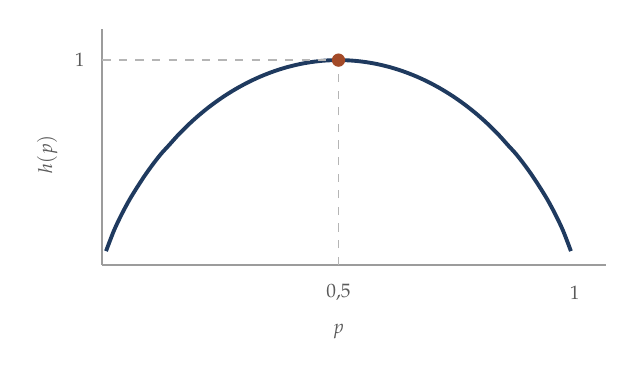
\begin{tikzpicture}[scale=1.0]
\draw[grau!60, line width=0.7pt] (0,0) -- (6.4,0);
\draw[grau!60, line width=0.7pt] (0,0) -- (0,3.0);
\draw[tief, line width=1.4pt, smooth, samples=60, domain=0.008:0.992]
  plot ({6*\x}, {2.6*(-\x*ln(\x)/ln(2) - (1-\x)*ln(1-\x)/ln(2))});
\draw[grau!45, line width=0.5pt, dashed] (0,2.6) -- (3,2.6);
\draw[grau!45, line width=0.5pt, dashed] (3,0) -- (3,2.6);
\fill[akzent] (3,2.6) circle (2.4pt);
\node[font=\scriptsize, color=grau, anchor=east] at (-0.1,2.6) {$1$};
\node[font=\scriptsize, color=grau] at (3,-0.35) {$0{,}5$};
\node[font=\scriptsize, color=grau] at (6,-0.35) {$1$};
\node[font=\scriptsize, color=grau] at (3.0,-0.85) {$p$};
\node[font=\scriptsize, color=grau, rotate=90] at (-0.7,1.4) {$h(p)$};
\end{tikzpicture}
\end{center}

\schritt{Drei Eigenschaften}
\begin{center}
{\small
\renewcommand{\arraystretch}{1.5}
\begin{tabular}{@{}P{2.4cm}P{6.2cm}@{}}
\toprule
\textbf{Symmetrie} & $h(p) = h(1-p)$ --- es ist gleichgültig, welchen Ausgang man \enquote{Erfolg} nennt.\\
\textbf{Maximum} & bei $p=\frac12$ mit dem Wert $1$.\\
\textbf{Steilheit} & An den Rändern ist die Kurve \kursiv{unendlich} steil: $h'(p)\to\infty$ für $p\to0$.\\
\bottomrule
\end{tabular}}
\end{center}

\kursiv{Zur dritten Zeile:}
\[ h'(p) = \lb\frac{1-p}{p} \ \longrightarrow\ \infty \quad\text{für } p\to0 \]

\begin{center}
\begin{minipage}{0.88\textwidth}
\kursiv{Das hat eine praktische Folge: Bei $p = 0{,}11$ ist $h = 0{,}5$ --- eine Münze, die nur in elf von hundert Fällen Kopf zeigt, trägt immer noch ein halbes Bit. \textbf{Um die Entropie zu halbieren, muss man die Wahrscheinlichkeit auf ein Neuntel drücken.} Seltene Ereignisse tragen mehr zur Ungewissheit bei, als man vermutet.}
\end{minipage}
\end{center}
\end{merksatz}

\section{Mehrere Größen}

\begin{definition}
\boxtitelm{Definition 2.4}
Für zwei Zufallsgrößen $X$ und $Y$ mit gemeinsamer Verteilung $p(x,y)$:
\begin{center}
{\small
\renewcommand{\arraystretch}{1.6}
\begin{tabular}{@{}P{2.8cm}P{5.6cm}@{}}
\toprule
\textbf{Verbundentropie} & $\Ent(X,Y) = -\sum_{x,y} p(x,y)\,\lb p(x,y)$\\
\textbf{Bedingte Entropie} & $\Ent(Y\mid X) = \sum_x p(x)\,\Ent(Y\mid X=x)$\\
\bottomrule
\end{tabular}}
\end{center}
\end{definition}

\begin{merksatz}
\boxtitel{Satz 2.5 --- die Kettenregel}
\[ \Ent(X,Y) = \Ent(X) + \Ent(Y\mid X) \]

\schritt{Beweis}
Mit $p(x,y) = p(x)\,p(y\mid x)$ und der Rechenregel für Logarithmen:
\begin{align*}
\Ent(X,Y) &= -\sum_{x,y} p(x,y)\,\lb\bigl(p(x)\,p(y\mid x)\bigr)\\
&= -\sum_{x,y} p(x,y)\,\lb p(x) \;-\; \sum_{x,y} p(x,y)\,\lb p(y\mid x)
\end{align*}

\kursiv{Erster Summand:} Über $y$ summieren ergibt $\sum_y p(x,y) = p(x)$:
\[ -\sum_x p(x)\,\lb p(x) = \Ent(X) \]

\kursiv{Zweiter Summand:} Mit $p(x,y) = p(x)p(y\mid x)$:
\[ -\sum_x p(x)\sum_y p(y\mid x)\,\lb p(y\mid x) = \sum_x p(x)\,\Ent(Y\mid X=x) = \Ent(Y\mid X) \]
$\blacksquare$

\begin{center}
\begin{minipage}{0.9\textwidth}
\textbf{In Worten: Die Ungewissheit über beides ist die Ungewissheit über das eine plus die verbleibende über das andere.}
\end{minipage}
\end{center}
\end{merksatz}

\begin{merksatz}
\boxtitel{Satz 2.6 --- Bedingen verringert die Entropie}
\[ \Ent(Y\mid X) \ \le\ \Ent(Y) \]
mit Gleichheit genau dann, wenn $X$ und $Y$ unabhängig sind.

\begin{center}
\begin{minipage}{0.9\textwidth}
\textbf{Zusätzliches Wissen kann die Ungewissheit nur verringern, nie vergrößern.}
\end{minipage}
\end{center}

\begin{center}
\begin{minipage}{0.88\textwidth}
\kursiv{Der Beweis läuft wie bei Satz 2.2 über die Jensensche Ungleichung; wir führen ihn in Kapitel~4, wo die Differenz $\Ent(Y)-\Ent(Y\mid X)$ ihren Namen erhält. \textbf{Vorsicht bei der Deutung:} Der Satz gilt für den \kursiv{Mittelwert} über alle $x$. Ein einzelnes $\Ent(Y\mid X=x)$ kann sehr wohl größer sein als $\Ent(Y)$ --- eine bestimmte Beobachtung kann verwirren, obwohl Beobachtungen im Mittel klären.}
\end{minipage}
\end{center}
\end{merksatz}

\begin{merksatz}
\boxtitel{Der Leitfall mit zwei Größen}
$X$: Gehört der Fall zur Gruppe $A$? $Y$: Ist der Laborwert positiv?

\begin{center}
{\small
\renewcommand{\arraystretch}{1.5}
\begin{tabular}{@{}P{2.0cm}P{1.8cm}P{1.8cm}P{1.8cm}@{}}
\toprule
& $Y=+$ & $Y=-$ & \textbf{Summe}\\
\midrule
$X=A$ & $0{,}125$ & $0{,}125$ & $0{,}250$\\
$X=\bar A$ & $0{,}075$ & $0{,}675$ & $0{,}750$\\
\midrule
\textbf{Summe} & $0{,}200$ & $0{,}800$ & $1{,}000$\\
\bottomrule
\end{tabular}}
\end{center}

\schritt{Die Randentropien}
\[ \Ent(X) = h(0{,}25) = 0{,}8113 \ \text{Bit} \]
\[ \Ent(Y) = h(0{,}20) = 0{,}7219 \ \text{Bit} \]

\schritt{Die bedingte Entropie}
\[ \Pr[Y=+\mid X=A] = \frac{0{,}125}{0{,}250} = 0{,}5, \qquad \Pr[Y=+\mid X=\bar A] = \frac{0{,}075}{0{,}750} = 0{,}1 \]
\[ \Ent(Y\mid X) = 0{,}25\cdot h(0{,}5) + 0{,}75\cdot h(0{,}1) = 0{,}25\cdot1 + 0{,}75\cdot0{,}4690 = 0{,}6017 \]

\schritt{Die Verbundentropie}
\kursiv{Direkt:}
\[ \Ent(X,Y) = -\bigl[2\cdot0{,}125\,\lb 0{,}125 + 0{,}075\,\lb 0{,}075 + 0{,}675\,\lb 0{,}675\bigr] \]
\[ = 0{,}750 + 0{,}2802 + 0{,}3828 = 1{,}4130 \ \text{Bit} \]

\kursiv{Über die Kettenregel:}
\[ \Ent(X) + \Ent(Y\mid X) = 0{,}8113 + 0{,}6017 = 1{,}4130 \quad \checkmark \]

\schritt{Die Bilanz}
\begin{center}
{\small
\renewcommand{\arraystretch}{1.48}
\begin{tabular}{@{}P{2.4cm}P{2.0cm}P{3.0cm}@{}}
\toprule
\textbf{Größe} & \textbf{Bit} & \\
\midrule
$\Ent(X)$ & $0{,}8113$ & \\
$\Ent(Y)$ & $0{,}7219$ & \\
$\Ent(X,Y)$ & $1{,}4130$ & \\
$\Ent(Y\mid X)$ & $0{,}6017$ & $< \Ent(Y)$ \checkmark\\
$\Ent(X\mid Y)$ & $0{,}6911$ & $< \Ent(X)$ \checkmark\\
\midrule
Summe der Ränder & $1{,}5332$ & $> \Ent(X,Y)$\\
\textbf{Differenz} & $\mathbf{0{,}1202}$ & \textcolor{akzent}{die Überschneidung}\\
\bottomrule
\end{tabular}}
\end{center}

\begin{center}
\begin{minipage}{0.9\textwidth}
\textbf{Die Verbundentropie ist kleiner als die Summe der Einzelentropien --- um $0{,}12$ Bit.} Das ist die Information, die beide Größen gemeinsam haben.
\end{minipage}
\end{center}

\begin{center}
\begin{minipage}{0.88\textwidth}
\kursiv{Es ist genau der Betrag, der in Kapitel~1 \enquote{verschwunden} war. Der Laborwert verrät etwas über die Diagnosegruppe und umgekehrt --- $0{,}12$ Bit, in beide Richtungen gleich viel. Kapitel~4 zeigt, dass diese Symmetrie kein Zufall ist.}
\end{minipage}
\end{center}
\end{merksatz}

\section{Der Bruchfall}

\begin{warnung}
\boxtitelr{Was die Entropie nicht sagt}
\begin{center}
{\small
\renewcommand{\arraystretch}{1.52}
\begin{tabular}{@{}P{2.4cm}P{6.2cm}@{}}
\toprule
\textbf{Keine Ordnung} & Die Entropie hängt nur von der \kursiv{Menge} der Wahrscheinlichkeiten ab, nicht davon, welcher Wert welche hat. Eine Vertauschung ändert nichts.\\
\textbf{Kein Abstand} & Ob die Werte $1,2,3$ oder $1, 100, 10^6$ heißen, ist gleichgültig. Für Zahlengrößen ist das oft die falsche Beschreibung.\\
\textbf{Keine Struktur} & Eine Folge, die aus lauter Wiederholungen besteht, kann dieselbe Entropie haben wie eine zufällige --- wenn man nur die Einzelhäufigkeiten betrachtet.\\
\bottomrule
\end{tabular}}
\end{center}

\schritt{Zur dritten Zeile}
Die Folge
\[ 010101010101\ldots \]
hat je zur Hälfte Nullen und Einsen, also eine Symbolentropie von einem Bit --- obwohl sie vollkommen vorhersehbar ist.

\begin{center}
\begin{minipage}{0.9\textwidth}
\textbf{Die Entropie einer Quelle ist nicht die Entropie ihrer Einzelsymbole.} Sie muss über immer längere Blöcke gemessen werden.
\end{minipage}
\end{center}

\begin{center}
\begin{minipage}{0.88\textwidth}
\kursiv{Bei Paaren ergibt sich für obige Folge nur noch ein halbes Bit je Symbol, bei Vierergruppen ein Viertel --- und im Grenzwert null. Man nennt das die \Begriff{Entropierate}; sie ist die richtige Größe für Quellen mit Gedächtnis und wird in Kapitel~3 eingeführt. \textbf{Deutscher Text hat eine Symbolentropie von etwa $4{,}1$ Bit und eine Entropierate von unter $1{,}5$ Bit je Zeichen} --- der Unterschied ist die Struktur der Sprache.}
\end{minipage}
\end{center}
\end{warnung}

\begin{warnung}
\boxtitelr{Und die stetige Fassung hat eine Falle}
Für eine stetige Größe mit Dichte $f$ definiert man
\[ \Ent(X) = -\int f(x)\,\lb f(x)\,\dd x . \]

\begin{center}
{\small
\renewcommand{\arraystretch}{1.5}
\begin{tabular}{@{}P{2.4cm}P{6.2cm}@{}}
\toprule
\textbf{Kann negativ sein} & Bei einer Gleichverteilung auf $[0;\ 0{,}5]$ ist $f=2$ und $\Ent = -1$ Bit.\\
\textbf{Nicht invariant} & Eine Skalierung $X \to aX$ ändert den Wert um $\lb a$.\\
\textbf{Kein Grenzwert} & Sie ist \kursiv{nicht} der Grenzwert der diskreten Entropie feiner werdender Einteilungen --- der wäre unendlich.\\
\bottomrule
\end{tabular}}
\end{center}

\begin{center}
\begin{minipage}{0.88\textwidth}
\kursiv{Man nennt sie deshalb genauer \Begriff{differentielle Entropie} und behandelt sie als eigenen Begriff. Die guten Eigenschaften bleiben dort erhalten, wo \kursiv{Differenzen} gebildet werden --- und genau das geschieht bei der Transinformation in Kapitel~4. Sie ist auch im stetigen Fall nichtnegativ und skaleninvariant.}
\end{minipage}
\end{center}
\end{warnung}

\section{Übungsaufgaben}

\begin{aufgabe}
\boxtitel{Aufgabe 2.1 --- Entropien vergleichen}
Berechnen Sie die Entropie und vergleichen Sie mit der oberen Schranke:
\begin{center}
{\small
\renewcommand{\arraystretch}{1.4}
\begin{tabular}{@{}P{0.8cm}P{7.6cm}@{}}
\toprule
(a) & Ein fairer Würfel.\\
(b) & Ein gezinkter Würfel: die Sechs mit $\frac12$, die übrigen gleich.\\
(c) & Ein Buchstabe aus $26$ gleich häufigen.\\
(d) & Die Blutgruppen: $0$ mit $0{,}41$, $A$ mit $0{,}43$, $B$ mit $0{,}11$, $AB$ mit $0{,}05$.\\
\bottomrule
\end{tabular}}
\end{center}

\loesung
\schritt{(a) Fairer Würfel}
Gleichverteilung, also Maximum:
\[ \Ent = \lb 6 = 2{,}585 \ \text{Bit} \]

\schritt{(b) Gezinkter Würfel}
Die Sechs hat $\frac12$, die übrigen fünf je $\frac{1}{10}$.
\[ \Ent = \tfrac12\lb2 + 5\cdot\tfrac1{10}\lb10 = 0{,}5 + 0{,}5\cdot3{,}3219 = 0{,}5+1{,}6610 = 2{,}161 \ \text{Bit} \]

\kursiv{Vergleich:} $2{,}161$ gegen $2{,}585$ --- eine Einbuße von $16{,}4$ Prozent.

\begin{center}
\begin{minipage}{0.86\textwidth}
\kursiv{Bemerkenswert wenig für eine so grobe Verfälschung: Die Sechs kommt dreifach zu häufig, und die Entropie sinkt um ein Sechstel. Das ist die Unempfindlichkeit aus Abschnitt 2.2.}
\end{minipage}
\end{center}

\schritt{(c) Buchstaben}
\[ \Ent = \lb 26 = \frac{\ln 26}{\ln 2} = \frac{3{,}2581}{0{,}6931} = 4{,}700 \ \text{Bit} \]

\begin{center}
\begin{minipage}{0.86\textwidth}
\kursiv{Deutscher Text erreicht diesen Wert bei weitem nicht: Die tatsächlichen Buchstabenhäufigkeiten ergeben etwa $4{,}1$ Bit, und unter Berücksichtigung der Abhängigkeiten sinkt der Wert auf unter $1{,}5$ Bit je Zeichen.}
\end{minipage}
\end{center}

\schritt{(d) Blutgruppen}
\begin{center}
\renewcommand{\arraystretch}{1.46}
\begin{tabular}{@{}P{1.6cm}P{1.6cm}P{2.0cm}P{2.0cm}@{}}
\toprule
& $p$ & $\lb(1/p)$ & $p\cdot\lb(1/p)$\\
\midrule
$0$ & $0{,}41$ & $1{,}2863$ & $0{,}5274$\\
$A$ & $0{,}43$ & $1{,}2176$ & $0{,}5236$\\
$B$ & $0{,}11$ & $3{,}1844$ & $0{,}3503$\\
$AB$ & $0{,}05$ & $4{,}3219$ & $0{,}2161$\\
\midrule
& $1{,}00$ & & $\mathbf{1{,}617}$\\
\bottomrule
\end{tabular}
\end{center}

\kursiv{Obere Schranke:} $\lb 4 = 2$ Bit.

\schritt{Die Übersicht}
\begin{center}
{\small
\renewcommand{\arraystretch}{1.48}
\begin{tabular}{@{}P{1.0cm}P{1.8cm}P{1.8cm}P{2.0cm}@{}}
\toprule
& $\Ent$ & $\lb n$ & \textbf{Ausnutzung}\\
\midrule
(a) & $2{,}585$ & $2{,}585$ & $100{,}0\,\%$\\
(b) & $2{,}161$ & $2{,}585$ & $83{,}6\,\%$\\
(c) & $4{,}700$ & $4{,}700$ & $100{,}0\,\%$\\
(d) & $1{,}617$ & $2{,}000$ & $80{,}9\,\%$\\
\bottomrule
\end{tabular}}
\end{center}

\begin{center}
\begin{minipage}{0.88\textwidth}
\kursiv{Die letzte Spalte ist die interessante: Sie gibt an, wie viel der möglichen Ungewissheit tatsächlich vorhanden ist. Ihr Gegenstück $1-\text{Ausnutzung}$ heißt \Begriff{Redundanz} --- bei den Blutgruppen also $19$ Prozent. Genau so viel lässt sich durch Codierung einsparen.}
\end{minipage}
\end{center}
\end{aufgabe}

\begin{aufgabe}
\boxtitel{Aufgabe 2.2 --- Die Kettenregel prüfen}
Für die Verbundverteilung
\begin{center}
{\small
\renewcommand{\arraystretch}{1.44}
\begin{tabular}{@{}P{1.8cm}P{1.6cm}P{1.6cm}P{1.6cm}@{}}
\toprule
& $y_1$ & $y_2$ & $y_3$\\
\midrule
$x_1$ & $\tfrac18$ & $\tfrac1{16}$ & $\tfrac1{16}$\\
$x_2$ & $\tfrac1{16}$ & $\tfrac18$ & $\tfrac1{16}$\\
$x_3$ & $\tfrac1{16}$ & $\tfrac1{16}$ & $\tfrac38$\\
\bottomrule
\end{tabular}}
\end{center}
berechnen Sie alle Entropien und prüfen Sie die Kettenregel.

\loesung
\schritt{Schritt 1 --- Die Ränder}
\begin{center}
\renewcommand{\arraystretch}{1.46}
\begin{tabular}{@{}P{1.6cm}P{2.6cm}P{2.0cm}@{}}
\toprule
& \textbf{Summe} & \textbf{Wert}\\
\midrule
$p(x_1)$ & $\tfrac18+\tfrac1{16}+\tfrac1{16}$ & $\tfrac14$\\
$p(x_2)$ & $\tfrac1{16}+\tfrac18+\tfrac1{16}$ & $\tfrac14$\\
$p(x_3)$ & $\tfrac1{16}+\tfrac1{16}+\tfrac38$ & $\tfrac12$\\
\bottomrule
\end{tabular}
\end{center}

Aus Symmetrie der Tabelle gilt dasselbe für $Y$.

\schritt{Schritt 2 --- Die Randentropien}
\[ \Ent(X) = 2\cdot\tfrac14\lb4 + \tfrac12\lb2 = 2\cdot0{,}5 + 0{,}5 = 1{,}5 \ \text{Bit} \]
Ebenso $\Ent(Y) = 1{,}5$ Bit.

\schritt{Schritt 3 --- Die Verbundentropie}
Die neun Felder: viermal $\frac1{16}$? Zählen wir nach:
\begin{center}
\renewcommand{\arraystretch}{1.46}
\begin{tabular}{@{}P{1.8cm}P{1.6cm}P{2.0cm}P{2.2cm}@{}}
\toprule
\textbf{Wert} & \textbf{Anzahl} & $\lb(1/p)$ & \textbf{Beitrag}\\
\midrule
$\tfrac18$ & $2$ & $3$ & $2\cdot\tfrac38 = 0{,}750$\\
$\tfrac1{16}$ & $6$ & $4$ & $6\cdot\tfrac14 = 1{,}500$\\
$\tfrac38$ & $1$ & $1{,}4150$ & $0{,}5306$\\
\midrule
\textbf{Summe} & & & $\mathbf{2{,}781}$\\
\bottomrule
\end{tabular}
\end{center}

\kursiv{Probe der Wahrscheinlichkeiten:} $2\cdot\tfrac18 + 6\cdot\tfrac1{16} + \tfrac38 = \tfrac14+\tfrac38+\tfrac38 = 1$ \checkmark

\kursiv{Zum dritten Beitrag:} $\lb\frac{8}{3} = 3 - \lb 3 = 3-1{,}5850 = 1{,}4150$; $0{,}375\cdot1{,}4150 = 0{,}5306$.

\schritt{Schritt 4 --- Die bedingte Entropie}
\kursiv{Gegeben $x_1$:} Die bedingten Wahrscheinlichkeiten sind $\frac{1/8}{1/4} = \frac12$ und zweimal $\frac{1/16}{1/4} = \frac14$.
\[ \Ent(Y\mid x_1) = \tfrac12\cdot1 + 2\cdot\tfrac14\cdot2 = 0{,}5+1{,}0 = 1{,}5 \]
Ebenso $\Ent(Y\mid x_2) = 1{,}5$.

\kursiv{Gegeben $x_3$:} $\frac{1/16}{1/2} = \frac18$ zweimal und $\frac{3/8}{1/2} = \frac34$.
\[ \Ent(Y\mid x_3) = 2\cdot\tfrac18\cdot3 + \tfrac34\lb\tfrac43 = 0{,}750 + 0{,}75\cdot0{,}4150 = 0{,}750+0{,}3113 = 1{,}0613 \]

\[ \Ent(Y\mid X) = \tfrac14\cdot1{,}5 + \tfrac14\cdot1{,}5 + \tfrac12\cdot1{,}0613 = 0{,}375+0{,}375+0{,}5306 = 1{,}2806 \]

\schritt{Schritt 5 --- Die Kettenregel prüfen}
\[ \Ent(X) + \Ent(Y\mid X) = 1{,}5 + 1{,}2806 = \mathbf{2{,}781} \quad \checkmark \]

\schritt{Schritt 6 --- Satz 2.6 prüfen}
\[ \Ent(Y\mid X) = 1{,}281 \ \le\ 1{,}500 = \Ent(Y) \quad \checkmark \]

\begin{center}
\begin{minipage}{0.88\textwidth}
\kursiv{Beachten Sie Schritt 4: Für $x_1$ und $x_2$ ist die bedingte Entropie \kursiv{genau so groß} wie $\Ent(Y)$ --- diese Beobachtungen klären nichts. Erst $x_3$ senkt sie deutlich. \textbf{Der Satz gilt im Mittel; einzelne Beobachtungen können wirkungslos sein.}}
\end{minipage}
\end{center}

\schritt{Schritt 7 --- Die Überschneidung}
\[ \Ent(X)+\Ent(Y)-\Ent(X,Y) = 1{,}5+1{,}5-2{,}781 = \mathbf{0{,}219} \ \text{Bit} \]
\end{aufgabe}

\begin{aufgabe}
\boxtitel{Aufgabe 2.3 --- Die Gruppierungseigenschaft}
Zeigen Sie: Fasst man zwei Werte mit den Wahrscheinlichkeiten $p_1$ und $p_2$ zu einem zusammen, so gilt
\[ \Ent(p_1,p_2,p_3,\ldots) = \Ent(p_1{+}p_2,\ p_3,\ldots) + (p_1{+}p_2)\,h\!\left(\frac{p_1}{p_1+p_2}\right) . \]
Prüfen Sie die Formel am Leitfall.

\loesung
\schritt{Schritt 1 --- Die Idee}
Man erfährt die Nachricht in zwei Schritten: erst, ob sie in der zusammengefassten Gruppe liegt, dann gegebenenfalls welcher der beiden Werte es ist.

\schritt{Schritt 2 --- Der Beweis}
Sei $q = p_1+p_2$. Die beiden fraglichen Summanden auf der linken Seite:
\[ -p_1\lb p_1 - p_2\lb p_2 \]

Wir schreiben $p_1 = q\cdot\frac{p_1}{q}$ und entsprechend $p_2$:
\begin{align*}
-p_1\lb p_1 &= -p_1\left(\lb q + \lb\tfrac{p_1}{q}\right) = -p_1\lb q - p_1\lb\tfrac{p_1}{q}\\
-p_2\lb p_2 &= -p_2\lb q - p_2\lb\tfrac{p_2}{q}
\end{align*}

Addieren:
\[ -(p_1+p_2)\lb q \;-\; q\left[\tfrac{p_1}{q}\lb\tfrac{p_1}{q} + \tfrac{p_2}{q}\lb\tfrac{p_2}{q}\right] = -q\lb q + q\,h\!\left(\tfrac{p_1}{q}\right) \]

Der erste Term ist genau der Beitrag des zusammengefassten Werts. $\blacksquare$

\schritt{Schritt 3 --- Am Leitfall}
Wir fassen $E$ und $F$ (je $0{,}0625$) zu einer Gruppe mit $0{,}125$ zusammen.

\kursiv{Links:} $\Ent = 2{,}75$ (acht Gruppen).

\kursiv{Rechts, erster Teil:} Sieben Gruppen mit $(0{,}25;\ 0{,}25;\ 0{,}125;\ 0{,}125;\ \mathbf{0{,}125};\ 0{,}0625;\ 0{,}0625)$:
\[ \Ent = 2\cdot0{,}5 + 3\cdot(0{,}125\cdot3) + 2\cdot(0{,}0625\cdot4) = 1{,}0 + 1{,}125 + 0{,}5 = 2{,}625 \]

\kursiv{Rechts, zweiter Teil:}
\[ 0{,}125 \cdot h\!\left(\tfrac{0{,}0625}{0{,}125}\right) = 0{,}125 \cdot h(0{,}5) = 0{,}125 \cdot 1 = 0{,}125 \]

\[ 2{,}625 + 0{,}125 = \mathbf{2{,}750} \quad \checkmark \]

\schritt{Schritt 4 --- Wozu das dient}
\begin{center}
{\small
\renewcommand{\arraystretch}{1.5}
\begin{tabular}{@{}P{3.0cm}P{5.6cm}@{}}
\toprule
\textbf{Codierung} & Das Huffman-Verfahren in Kapitel~3 fasst genau so zusammen --- und die Formel sagt, was das kostet.\\
\textbf{Entscheidungs\-bäume} & In der Statistik wählt man Aufteilungen nach dem Entropiegewinn; die Formel ist die Rechengrundlage.\\
\textbf{Axiomatik} & Zusammen mit Stetigkeit und dem Wert $h(\frac12)=1$ legt sie die Entropie vollständig fest.\\
\bottomrule
\end{tabular}}
\end{center}

\begin{center}
\begin{minipage}{0.88\textwidth}
\kursiv{Die dritte Zeile ist Shannons eigener Zugang von 1948: Er forderte Stetigkeit, Monotonie im Umfang bei Gleichverteilung und genau diese Gruppierungseigenschaft --- und bewies, dass nur $-C\sum p_i\ln p_i$ übrigbleibt. Es ist derselbe Aufbau wie bei Satz 1.1, nur eine Ebene höher.}
\end{minipage}
\end{center}
\end{aufgabe}

\begin{geschichte}
\boxtitelg{Eine Formel mit zwei Herkünften}
Die Funktion $-\sum p_i\ln p_i$ stand in der Physik, bevor sie in der Nachrichtentechnik auftauchte.

\schritt{Boltzmann, 1877}
\Person{Ludwig Boltzmann} (1844--1906) verband die thermodynamische Entropie mit der Zahl $W$ der mikroskopischen Zustände, die zu einem makroskopischen gehören:
\[ S = k_B \ln W \]

\begin{center}
\begin{minipage}{0.9\textwidth}
\kursiv{Das ist der Sonderfall gleich wahrscheinlicher Zustände --- genau Hartleys Formel aus Kapitel~1, nur in anderer Einheit. Die Gleichung steht auf Boltzmanns Grabstein in Wien, obwohl er sie in dieser Form nie aufschrieb; \Person{Max Planck} gab ihr die heutige Gestalt.}
\end{minipage}
\end{center}

\schritt{Gibbs, 1902}
\Person{Josiah Willard Gibbs} verallgemeinerte auf ungleiche Wahrscheinlichkeiten:
\[ S = -k_B\sum_i p_i \ln p_i \]

\begin{center}
\begin{minipage}{0.9\textwidth}
\kursiv{Das ist Shannons Formel, sechsundvierzig Jahre früher und mit einer physikalischen Konstante davor. Dass beide Größen dieselbe Gestalt haben, ist kein Zufall: Beide zählen, wie viele Möglichkeiten es gibt --- die eine für Moleküle, die andere für Nachrichten.}
\end{minipage}
\end{center}

\schritt{Der Zusammenhang}
\Person{Leó Szilárd} zeigte 1929 an einem Gedankenexperiment, dass der Maxwellsche Dämon --- ein Wesen, das Moleküle sortiert und damit angeblich den zweiten Hauptsatz verletzt --- genau dann keine Arbeit gewinnt, wenn man den Informationsgewinn mitbilanziert.

\begin{center}
\begin{minipage}{0.9\textwidth}
\kursiv{Ein Bit Information entspricht dabei der Entropie $k_B\ln 2$. Die Auflösung des Paradoxons vollendete \Person{Charles Bennett} 1982: Nicht das Messen kostet, sondern das \kursiv{Löschen} des Gedächtnisses --- nach dem Landauer-Prinzip aus Kapitel~1.}
\end{minipage}
\end{center}

\schritt{Und eine Warnung}
\begin{center}
\begin{minipage}{0.9\textwidth}
\kursiv{Die Gleichheit der Formeln hat zu weitreichenden Behauptungen geführt --- über Information als physikalische Grundgröße, über das Universum als Rechner. Der sichere Kern ist schmaler: Beide Größen zählen Möglichkeiten, und wo eine physikalische Fragestellung auf ein Abzählen von Zuständen hinausläuft, tritt dieselbe Funktion auf. Mehr folgt daraus nicht von selbst.}
\end{minipage}
\end{center}
\end{geschichte}

\begin{forschung}
\boxtitelp{Entropie als Werkzeug}
\begin{center}
{\small
\renewcommand{\arraystretch}{1.45}
\begin{tabular}{@{}P{3.2cm}P{5.0cm}@{}}
\toprule
\textbf{Maximale Entropie} & Unter allen Verteilungen mit gegebenen Erwartungswerten diejenige mit größter Entropie wählen --- das Prinzip der geringsten Zusatzannahme.\\
\textbf{Entscheidungs\-bäume} & Aufteilungen werden nach dem Entropiegewinn gewählt.\\
\textbf{Schätzung} & Die Entropie aus Daten zu schätzen ist bei vielen Symbolen systematisch verzerrt --- nach unten.\\
\bottomrule
\end{tabular}}
\end{center}

\schritt{Zur ersten Zeile}
\Person{Edwin Jaynes} schlug 1957 vor, unter allen mit den Daten verträglichen Verteilungen die entropiereichste zu wählen.

\begin{center}
\begin{minipage}{0.88\textwidth}
\kursiv{Die Ergebnisse sind bemerkenswert: Gibt man nur den Mittelwert vor, so ergibt sich die Exponentialverteilung; gibt man Mittelwert und Varianz vor, die Normalverteilung. \textbf{Die Normalverteilung ist also die Verteilung, die bei gegebener Streuung am wenigsten behauptet} --- eine Begründung für ihre Sonderstellung, die neben dem zentralen Grenzwertsatz aus Band 12 steht.}
\end{minipage}
\end{center}

\schritt{Zur dritten Zeile}
Schätzt man $\Ent$ durch Einsetzen der beobachteten Häufigkeiten, so ist das Ergebnis zu klein.

\begin{center}
\begin{minipage}{0.88\textwidth}
\kursiv{Der Grund ist Jensen: Die Entropie ist eine konkave Funktion der Wahrscheinlichkeiten, und der Erwartungswert einer konkaven Funktion liegt unter der Funktion des Erwartungswerts. Der Fehler beträgt näherungsweise $\frac{n-1}{2N\ln 2}$ Bit bei $n$ Symbolen und $N$ Beobachtungen --- bei vielen seltenen Symbolen also erheblich. Es ist derselbe Sachverhalt wie in Band 19, Kapitel~13, nur mit umgekehrtem Vorzeichen.}
\end{minipage}
\end{center}
\end{forschung}

\begin{merksatz}
\boxtitel{Was Sie jetzt können}
\begin{center}
\renewcommand{\arraystretch}{1.5}
\begin{tabular}{@{}P{3.0cm}P{5.6cm}@{}}
\toprule
\textbf{Definition 2.1} & $\Ent = -\sum p_i\lb p_i$\\
\textbf{Satz 2.2} & $0 \le \Ent \le \lb n$, Jensen\\
\textbf{Definition 2.3} & $h(p)$, Maximum bei $\frac12$\\
\textbf{Satz 2.5} & Kettenregel\\
\textbf{Satz 2.6} & Bedingen verringert --- im Mittel\\
\bottomrule
\end{tabular}
\end{center}

\begin{center}
\begin{minipage}{0.88\textwidth}
\kursiv{Im nächsten Kapitel wird aus der Zahl $2{,}75$ ein Satz: Sie ist erreichbar, und weniger geht nicht.}
\end{minipage}
\end{center}
\end{merksatz}

\chapter{Quellencodierung}

\section{Was ein brauchbarer Code leisten muss}

\begin{merksatz}
\boxtitel{Das Problem der Trennung}
Wir wollen häufigen Gruppen kurze Codewörter geben. Aber:

\begin{center}
{\small
\renewcommand{\arraystretch}{1.48}
\begin{tabular}{@{}P{1.8cm}P{1.8cm}P{1.8cm}P{1.8cm}@{}}
\toprule
& $A$ & $B$ & $C$\\
\midrule
Code 1 & $0$ & $1$ & $01$\\
\bottomrule
\end{tabular}}
\end{center}

Die Folge $01$ kann $C$ bedeuten oder $AB$ --- der Code ist nicht eindeutig lesbar.

\schritt{Die Abhilfe}
\begin{center}
\begin{minipage}{0.9\textwidth}
\textbf{Kein Codewort darf Anfangsstück eines anderen sein.} Solche Codes heißen \Begriff{präfixfrei}.
\end{minipage}
\end{center}

\begin{center}
{\small
\renewcommand{\arraystretch}{1.48}
\begin{tabular}{@{}P{1.8cm}P{1.8cm}P{1.8cm}P{1.8cm}@{}}
\toprule
& $A$ & $B$ & $C$\\
\midrule
Code 2 & $0$ & $10$ & $11$\\
\bottomrule
\end{tabular}}
\end{center}

\kursiv{Probe:} $01011$ liest sich eindeutig als $0\mid10\mid11$, also $ABC$.

\begin{center}
\begin{minipage}{0.88\textwidth}
\kursiv{Präfixfreie Codes lassen sich ohne jedes Zurückblicken lesen: Sobald ein Codewort erkannt ist, steht es fest. Man nennt sie deshalb auch \kursiv{augenblicklich decodierbar}. Es gibt eindeutig lesbare Codes, die nicht präfixfrei sind --- aber wie Satz 3.1 zeigt, gewinnt man dadurch nichts.}
\end{minipage}
\end{center}
\end{merksatz}

\begin{merksatz}
\boxtitel{Der Codebaum}
Jeder präfixfreie Binärcode entspricht einem Baum: Links bedeutet $0$, rechts $1$, und die Codewörter sitzen an den Blättern.

\begin{center}
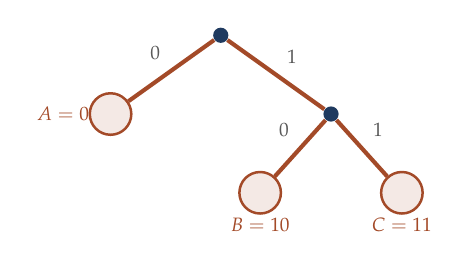
\begin{tikzpicture}[scale=1.0]
\node[knoten] (w) at (0,2.0) {};
\node[knotenr] (a) at (-1.4,1.0) {};
\node[knoten] (r) at (1.4,1.0) {};
\node[knotenr] (b) at (0.5,0.0) {};
\node[knotenr] (c) at (2.3,0.0) {};
\draw[kanted] (w)--(a) node[midway,above left,font=\scriptsize,color=grau] {$0$};
\draw[kanted] (w)--(r) node[midway,above right,font=\scriptsize,color=grau] {$1$};
\draw[kanted] (r)--(b) node[midway,above left,font=\scriptsize,color=grau] {$0$};
\draw[kanted] (r)--(c) node[midway,above right,font=\scriptsize,color=grau] {$1$};
\node[font=\scriptsize, color=akzent, anchor=east] at (-1.55,1.0) {$A = 0$};
\node[font=\scriptsize, color=akzent, anchor=north] at (0.5,-0.2) {$B = 10$};
\node[font=\scriptsize, color=akzent, anchor=north] at (2.3,-0.2) {$C = 11$};
\end{tikzpicture}
\end{center}

\begin{center}
\begin{minipage}{0.9\textwidth}
\textbf{Präfixfreiheit heißt: Kein Codewort liegt auf dem Weg zu einem anderen.} Alle sitzen an Blättern, keines an einem inneren Knoten.
\end{minipage}
\end{center}
\end{merksatz}

\section{Die Kraftsche Ungleichung}

\begin{merksatz}
\boxtitel{Satz 3.1 --- wann Wortlängen möglich sind}
Zu vorgegebenen Längen $l_1,\ldots,l_n$ gibt es genau dann einen präfixfreien Binärcode, wenn
\[ \sum_{i=1}^{n} 2^{-l_i} \ \le\ 1 . \]

\schritt{Beweis der Notwendigkeit}
Sei $L = \max_i l_i$ und der Code gegeben. Wir betrachten den vollständigen Binärbaum der Tiefe $L$ mit seinen $2^{L}$ Blättern.

\schritt{Schritt 1 --- was ein Codewort blockiert}
Ein Codewort der Länge $l_i$ sitzt an einem Knoten der Tiefe $l_i$. Unter diesem Knoten liegen genau
\[ 2^{\,L-l_i} \]
Blätter der Tiefe $L$.

\schritt{Schritt 2 --- die Bereiche sind getrennt}
Wären zwei dieser Blättermengen nicht disjunkt, so läge ein Codewort auf dem Weg zum anderen --- Widerspruch zur Präfixfreiheit.

\schritt{Schritt 3 --- abzählen}
Die Summe aller blockierten Blätter kann die Gesamtzahl nicht übersteigen:
\[ \sum_{i=1}^{n} 2^{\,L-l_i} \ \le\ 2^{L} \]
Division durch $2^{L}$ liefert die Behauptung. \checkmark

\schritt{Beweis der Hinlänglichkeit}
Sei die Ungleichung erfüllt. Wir ordnen die Längen aufsteigend: $l_1 \le l_2 \le \cdots \le l_n$ und vergeben die Codewörter der Reihe nach.

Vor der Vergabe des $k$-ten Wortes sind
\[ \sum_{i<k} 2^{\,L-l_i} \]
Blätter blockiert. Es bleiben
\[ 2^{L} - \sum_{i<k} 2^{\,L-l_i} \ \ge\ \sum_{i \ge k} 2^{\,L-l_i} \ \ge\ 2^{\,L-l_k} \]
Blätter frei --- also mindestens so viele, wie das $k$-te Wort benötigt. Da die Längen aufsteigend sind, lässt sich stets ein passender freier Knoten finden. $\blacksquare$

\begin{center}
\begin{minipage}{0.88\textwidth}
\kursiv{Der Satz übersetzt eine Aussage über Bäume in eine Ungleichung über Zahlen --- und macht sie damit dem Rechnen zugänglich. \textbf{Dieselbe Ungleichung gilt auch für eindeutig lesbare Codes}, die nicht präfixfrei sind; der Beweis dafür ist länger. Deshalb verliert man durch die Beschränkung auf Präfixcodes nichts.}
\end{minipage}
\end{center}
\end{merksatz}

\begin{merksatz}
\boxtitel{Die Ungleichung nachgerechnet}
\begin{center}
{\small
\renewcommand{\arraystretch}{1.48}
\begin{tabular}{@{}P{2.8cm}P{2.6cm}P{2.4cm}@{}}
\toprule
\textbf{Längen} & $\sum 2^{-l_i}$ & \\
\midrule
$1,2,2$ & $\tfrac12+\tfrac14+\tfrac14 = 1$ & \textcolor{gruen}{möglich}\\
$2,2,3,3,4,4,4,4$ & $1$ & \textcolor{gruen}{möglich}\\
$1,2,2,3$ & $\tfrac12+\tfrac14+\tfrac14+\tfrac18$ & \textcolor{akzent}{$>1$}\\
$2,2,3,4,5,5$ & $0{,}75$ & \textcolor{gruen}{möglich, mit Reserve}\\
\bottomrule
\end{tabular}}
\end{center}

\begin{center}
\begin{minipage}{0.9\textwidth}
\textbf{Gleichheit bedeutet, dass der Baum vollständig ausgenutzt ist.} Bleibt Reserve, so könnte man mindestens ein Codewort verkürzen.
\end{minipage}
\end{center}

\kursiv{Zur zweiten Zeile:} $2\cdot\frac14 + 2\cdot\frac18 + 4\cdot\frac1{16} = 0{,}5+0{,}25+0{,}25 = 1$. Das sind die Längen des Leitfalls.
\end{merksatz}

\section{Die untere Schranke}

\begin{merksatz}
\boxtitel{Satz 3.2 --- keine Codierung unterbietet die Entropie}
Für jeden präfixfreien Code mit den Wortlängen $l_i$ gilt
\[ L \ :=\ \sum_i p_i\,l_i \ \ge\ \Ent(X) . \]
Gleichheit gilt genau dann, wenn $l_i = -\lb p_i$ für alle $i$.

\schritt{Beweis --- Schritt 1: die Differenz}
\[ L - \Ent(X) = \sum_i p_i\,l_i + \sum_i p_i\,\lb p_i = \sum_i p_i\,\lb\bigl(p_i\,2^{\,l_i}\bigr) \]

\schritt{Schritt 2 --- Abkürzung}
Wir setzen $q_i := 2^{-l_i}$ und $Q := \sum_i q_i$. Nach Satz 3.1 ist $Q \le 1$.
\[ L - \Ent(X) = \sum_i p_i\,\lb\frac{p_i}{q_i} \]

\schritt{Schritt 3 --- Jensen}
Wir betrachten das Negative und wenden die Jensensche Ungleichung auf den konkaven Logarithmus an:
\begin{align*}
-\bigl(L-\Ent(X)\bigr) &= \sum_i p_i\,\lb\frac{q_i}{p_i}\\
&\le \lb\left(\sum_i p_i\cdot\frac{q_i}{p_i}\right) && \text{(Jensen)}\\
&= \lb Q \ \le\ \lb 1 = 0 && \text{(Satz 3.1)}
\end{align*}

Also $L - \Ent(X) \ge 0$. \checkmark

\schritt{Schritt 4 --- wann Gleichheit}
Es müssen \kursiv{beide} Ungleichungen mit Gleichheit gelten:
\begin{center}
\renewcommand{\arraystretch}{1.5}
\begin{tabular}{@{}P{2.4cm}P{6.2cm}@{}}
\toprule
\textbf{Jensen} & alle $\frac{q_i}{p_i}$ gleich, also $q_i = c\,p_i$\\
\textbf{Kraft} & $Q = 1$, also $c = 1$ und damit $q_i = p_i$\\
\bottomrule
\end{tabular}
\end{center}

Aus $q_i = 2^{-l_i} = p_i$ folgt $l_i = -\lb p_i$. $\blacksquare$

\begin{center}
\begin{minipage}{0.9\textwidth}
\textbf{Die Entropie ist erreichbar genau dann, wenn alle Wahrscheinlichkeiten Zweierpotenzen sind.} Dann ist $-\lb p_i$ ganzzahlig.
\end{minipage}
\end{center}

\begin{center}
\begin{minipage}{0.88\textwidth}
\kursiv{Das ist der Leitfall: $\frac14$, $\frac18$ und $\frac1{16}$ ergeben die Längen $2$, $3$ und $4$, und $L = \Ent = 2{,}75$. Man nennt solche Verteilungen \Begriff{dyadisch}. Für alle anderen bleibt eine Lücke --- und der nächste Satz sagt, wie groß sie höchstens ist.}
\end{minipage}
\end{center}
\end{merksatz}

\section{Die obere Schranke}

\begin{merksatz}
\boxtitel{Satz 3.3 --- der Quellencodierungssatz}
Es gibt stets einen präfixfreien Code mit
\[ \Ent(X) \ \le\ L \ <\ \Ent(X) + 1 . \]

\schritt{Beweis --- die Konstruktion}
Man wähle
\[ l_i := \left\lceil -\lb p_i \right\rceil . \]

\schritt{Schritt 1 --- Kraft ist erfüllt}
Aus $l_i \ge -\lb p_i$ folgt $2^{-l_i} \le 2^{\lb p_i} = p_i$, also
\[ \sum_i 2^{-l_i} \ \le\ \sum_i p_i = 1 . \]
Nach Satz 3.1 existiert ein solcher Code. \checkmark

\schritt{Schritt 2 --- die obere Abschätzung}
Aus $\lceil x\rceil < x+1$:
\[ L = \sum_i p_i\,l_i \ <\ \sum_i p_i\,(-\lb p_i + 1) = \Ent(X) + 1 \]

\schritt{Schritt 3 --- die untere}
Satz 3.2. $\blacksquare$

\begin{center}
\begin{minipage}{0.88\textwidth}
\kursiv{Die Konstruktion heißt Shannon-Code. Sie ist nicht die beste --- das Aufrunden verschenkt bei jeder Wahrscheinlichkeit etwas ---, aber sie \kursiv{beweist} die Schranke. Für den Beweis genügt ein Code, für die Praxis will man den besten.}
\end{minipage}
\end{center}
\end{merksatz}

\section{Das Huffman-Verfahren}

\begin{merksatz}
\boxtitel{Der Aufbau von unten}
\begin{center}
\renewcommand{\arraystretch}{1.5}
\begin{tabular}{@{}P{1.0cm}P{7.4cm}@{}}
\toprule
$1$ & Die beiden kleinsten Wahrscheinlichkeiten zusammenfassen.\\
$2$ & Die Summe als neues Symbol in die Liste aufnehmen.\\
$3$ & Wiederholen, bis nur noch ein Symbol übrig ist.\\
$4$ & Den entstandenen Baum von der Wurzel aus beschriften.\\
\bottomrule
\end{tabular}
\end{center}

\begin{center}
\begin{minipage}{0.88\textwidth}
\kursiv{Der Gedanke stammt aus Aufgabe 2.3: Das Zusammenfassen zweier Werte kostet genau $q\,h(p_1/q)$ zusätzliche Entropie. Huffman fasst stets dort zusammen, wo dieser Aufpreis am kleinsten ist --- bei den seltensten Symbolen.}
\end{minipage}
\end{center}
\end{merksatz}

\begin{merksatz}
\boxtitel{Ein Durchlauf}
Sechs Befundarten mit den Anteilen
\[ 0{,}40; \quad 0{,}25; \quad 0{,}15; \quad 0{,}10; \quad 0{,}06; \quad 0{,}04 \]

\schritt{Die Zusammenfassungen}
\begin{center}
{\small
\renewcommand{\arraystretch}{1.48}
\begin{tabular}{@{}P{1.1cm}P{3.0cm}P{3.7cm}@{}}
\toprule
\textbf{Runde} & \textbf{zusammen\-gefasst} & \textbf{neue Liste}\\
\midrule
$1$ & $0{,}06+0{,}04 = 0{,}10$ & $0{,}40;\ 0{,}25;\ 0{,}15;$ $0{,}10;\ 0{,}10$\\
$2$ & $0{,}10+0{,}10 = 0{,}20$ & $0{,}40;\ 0{,}25;\ 0{,}20;\ 0{,}15$\\
$3$ & $0{,}15+0{,}20 = 0{,}35$ & $0{,}40;\ 0{,}35;\ 0{,}25$\\
$4$ & $0{,}25+0{,}35 = 0{,}60$ & $0{,}60;\ 0{,}40$\\
$5$ & $0{,}40+0{,}60 = 1{,}00$ & fertig\\
\bottomrule
\end{tabular}}
\end{center}

\schritt{Die Wortlängen}
Jedes Symbol erhält so viele Bit, an wie vielen Zusammenfassungen es beteiligt war:
\begin{center}
{\small
\renewcommand{\arraystretch}{1.48}
\begin{tabular}{@{}P{1.6cm}P{1.8cm}P{1.6cm}P{2.2cm}@{}}
\toprule
$p$ & \textbf{Länge} & $p\cdot l$ & \\
\midrule
$0{,}40$ & $1$ & $0{,}40$ & \\
$0{,}25$ & $2$ & $0{,}50$ & \\
$0{,}15$ & $3$ & $0{,}45$ & \\
$0{,}10$ & $4$ & $0{,}40$ & \\
$0{,}06$ & $5$ & $0{,}30$ & \\
$0{,}04$ & $5$ & $0{,}20$ & \\
\midrule
& & $\mathbf{2{,}25}$ & \\
\bottomrule
\end{tabular}}
\end{center}

\kursiv{Kraft-Probe:} $\frac12+\frac14+\frac18+\frac1{16}+2\cdot\frac1{32} = 0{,}5+0{,}25+0{,}125+0{,}0625+0{,}0625 = 1$ \checkmark

\schritt{Der Vergleich}
\begin{center}
{\small
\renewcommand{\arraystretch}{1.48}
\begin{tabular}{@{}P{2.8cm}P{2.4cm}P{2.4cm}@{}}
\toprule
& \textbf{Längen} & $L$\\
\midrule
Entropie & --- & $2{,}201$\\
\textbf{Huffman} & $1,2,3,4,5,5$ & $\mathbf{2{,}250}$\\
Shannon-Code & $2,2,3,4,5,5$ & $2{,}650$\\
Gleiche Länge & $3,3,3,3,3,3$ & $3{,}000$\\
\bottomrule
\end{tabular}}
\end{center}

\kursiv{Zum Shannon-Code:} $\lceil-\lb0{,}40\rceil = \lceil1{,}32\rceil = 2$, $\lceil-\lb0{,}25\rceil = 2$, und so fort. Die Kraft-Summe beträgt nur $0{,}75$ --- es bleibt Reserve, also ist der Code nicht ausgereizt.

\begin{center}
\begin{minipage}{0.9\textwidth}
\textbf{Huffman liegt $2{,}2$ Prozent über der Entropie, der Shannon-Code $20{,}4$ Prozent.} Beide erfüllen Satz 3.3 --- aber der Unterschied ist erheblich.
\end{minipage}
\end{center}
\end{merksatz}

\begin{merksatz}
\boxtitel{Satz 3.4 --- Huffman ist optimal}
Kein präfixfreier Code hat eine kleinere mittlere Länge als der Huffman-Code.

\schritt{Die beiden tragenden Beobachtungen}
\begin{center}
{\small
\renewcommand{\arraystretch}{1.52}
\begin{tabular}{@{}P{1.0cm}P{7.4cm}@{}}
\toprule
$1$ & In einem optimalen Code haben die beiden seltensten Symbole die größte und dieselbe Länge.\\
$2$ & Sie können als Geschwister im Baum angeordnet werden, ohne die Länge zu ändern.\\
\bottomrule
\end{tabular}}
\end{center}

\kursiv{Zu 1:} Hätte ein selteneres Symbol ein kürzeres Wort als ein häufigeres, so würde Vertauschen die mittlere Länge senken. Und ein längstes Codewort muss ein Geschwister haben --- sonst könnte man sein letztes Bit streichen.

\schritt{Der Schluss}
Sind die beiden seltensten Geschwister, so ist der Code genau dann optimal für die ursprüngliche Verteilung, wenn der um sie verkürzte Code für die zusammengefasste Verteilung optimal ist.

\kursiv{Grund:} Nach Aufgabe 2.3 unterscheiden sich die mittleren Längen um genau $p_1+p_2$ --- unabhängig davon, wie der Rest codiert ist.

Damit ist das Problem auf eines mit einem Symbol weniger zurückgeführt, und Induktion liefert die Behauptung. $\blacksquare$

\begin{center}
\begin{minipage}{0.88\textwidth}
\kursiv{Bemerkenswert an diesem Beweis ist, was er nicht braucht: keine Analysis, keine Ungleichung, nur ein Vertauschungsargument und Induktion. \textbf{Huffman fand ihn 1951 als Student}, nachdem sein Lehrer Fano die Aufgabe als offenes Problem gestellt hatte.}
\end{minipage}
\end{center}
\end{merksatz}

\section{Blöcke codieren}

\begin{merksatz}
\boxtitel{Die Lücke verkleinern}
Satz 3.3 lässt bis zu einem Bit Verlust je Symbol zu. Bei kleiner Entropie ist das viel.

\schritt{Der Ausweg}
Man codiert nicht einzelne Symbole, sondern Blöcke der Länge $n$. Für unabhängige Symbole gilt
\[ \Ent(X_1,\ldots,X_n) = n\,\Ent(X) \]
und Satz 3.3 liefert
\[ n\,\Ent(X) \ \le\ L_n \ <\ n\,\Ent(X)+1 . \]

Je Symbol:
\[ \Ent(X) \ \le\ \frac{L_n}{n} \ <\ \Ent(X) + \frac1n \]

\begin{center}
\begin{minipage}{0.9\textwidth}
\textbf{Der Überhang schrumpft wie $1/n$ und geht gegen null.}
\end{minipage}
\end{center}

\schritt{Am Beispiel}
Eine Quelle liefert \enquote{unauffällig} mit $0{,}8$ und \enquote{auffällig} mit $0{,}2$. Die Entropie beträgt $h(0{,}2) = 0{,}7219$ Bit.

\begin{center}
{\small
\renewcommand{\arraystretch}{1.48}
\begin{tabular}{@{}P{1.4cm}P{2.0cm}P{2.0cm}P{2.2cm}@{}}
\toprule
$n$ & $L_n$ & $L_n/n$ & \textbf{Überhang}\\
\midrule
$1$ & $1{,}000$ & $1{,}0000$ & $0{,}2781$\\
$2$ & $1{,}560$ & $0{,}7800$ & $0{,}0581$\\
$3$ & $2{,}184$ & $0{,}7280$ & $\mathbf{0{,}0061}$\\
$4$ & $2{,}963$ & $0{,}7408$ & $0{,}0189$\\
$6$ & $4{,}351$ & $0{,}7253$ & $0{,}0033$\\
\bottomrule
\end{tabular}}
\end{center}

\begin{center}
\begin{minipage}{0.9\textwidth}
\textbf{Von $38$ Prozent Überhang bei Einzelcodierung auf unter ein Prozent bei Dreiergruppen.}
\end{minipage}
\end{center}

\begin{center}
\begin{minipage}{0.88\textwidth}
\kursiv{Beachten Sie, dass der Überhang \kursiv{nicht} monoton fällt: Bei $n=4$ ist er größer als bei $n=3$. Die Schranke $1/n$ gilt, der tatsächliche Wert schwankt darunter --- je nachdem, wie gut die Blockwahrscheinlichkeiten zufällig zu Zweierpotenzen passen. \textbf{Der Satz garantiert die Einhüllende, nicht den Verlauf.}}
\end{minipage}
\end{center}

\schritt{Der Preis}
Bei $n$ Symbolen und einem Alphabet der Größe $m$ hat die Codetabelle $m^{n}$ Einträge.

\begin{center}
\renewcommand{\arraystretch}{1.46}
\begin{tabular}{@{}P{1.6cm}P{2.2cm}P{2.6cm}@{}}
\toprule
$n$ & $2^{n}$ & $8^{n}$\\
\midrule
$3$ & $8$ & $512$\\
$6$ & $64$ & $262\,144$\\
$10$ & $1024$ & $10^{9}$\\
$20$ & $10^{6}$ & \textcolor{akzent}{$10^{18}$}\\
\bottomrule
\end{tabular}
\end{center}

\begin{center}
\begin{minipage}{0.88\textwidth}
\kursiv{Das ist der Grund, warum Huffman in der Praxis nicht auf lange Blöcke angewandt wird. Die arithmetische Codierung aus dem Forschungskasten umgeht das Problem: Sie erreicht die Entropie ohne Codetabelle, indem sie die gesamte Nachricht auf eine einzige Zahl abbildet.}
\end{minipage}
\end{center}
\end{merksatz}

\begin{merksatz}
\boxtitel{Quellen mit Gedächtnis}
Sind die Symbole abhängig, so ist $\Ent(X_1,\ldots,X_n) < n\,\Ent(X)$, und die richtige Größe ist die \Begriff{Entropierate}
\[ \Ent_\infty = \lim_{n\to\infty} \frac{\Ent(X_1,\ldots,X_n)}{n} . \]

\begin{center}
{\small
\renewcommand{\arraystretch}{1.48}
\begin{tabular}{@{}P{2.8cm}P{2.8cm}P{2.2cm}@{}}
\toprule
\textbf{Quelle} & \textbf{Symbol\-entropie} & \textbf{Rate}\\
\midrule
$010101\ldots$ & $1{,}00$ & $0{,}00$\\
Deutscher Text & $\approx4{,}1$ & $<1{,}5$\\
Gleichverteilt, $26$ & $4{,}70$ & $4{,}70$\\
\bottomrule
\end{tabular}}
\end{center}

\begin{center}
\begin{minipage}{0.88\textwidth}
\kursiv{Die zweite Zeile stammt aus Shannons Untersuchung von 1951, in der er Versuchspersonen den nächsten Buchstaben eines Textes raten ließ und aus ihrer Trefferquote die Rate abschätzte. Sie liegt bei etwa einem Bit je Zeichen --- \textbf{sprachlicher Text ist zu rund achtzig Prozent redundant.} Genau davon leben alle Textkompressionsverfahren.}
\end{minipage}
\end{center}
\end{merksatz}

\section{Der Bruchfall}

\begin{warnung}
\boxtitelr{Was der Satz nicht sagt}
\begin{center}
{\small
\renewcommand{\arraystretch}{1.52}
\begin{tabular}{@{}P{2.4cm}P{6.2cm}@{}}
\toprule
\textbf{Die Verteilung} & Sie muss bekannt sein. Wird sie aus den Daten geschätzt, so kostet das Speicherplatz für die Tabelle --- und die Schätzung ist verzerrt.\\
\textbf{Nur im Mittel} & Einzelne Nachrichten können länger werden als vorher. Nur der Erwartungswert sinkt.\\
\textbf{Keine Fehlertoleranz} & Ein einziges gekipptes Bit kann den ganzen Rest unlesbar machen --- der Code verliert den Tritt.\\
\bottomrule
\end{tabular}}
\end{center}

\schritt{Zur zweiten Zeile}
Im Beispiel erhält das seltenste Symbol fünf Bit statt drei bei gleicher Länge. Kommt es gehäuft vor, so ist die Nachricht länger.

\begin{center}
\begin{minipage}{0.9\textwidth}
\textbf{Es gibt keinen Code, der \kursiv{jede} Nachricht verkürzt.} Ein solcher müsste eine Abbildung sein, die eine endliche Menge in eine kleinere umkehrbar abbildet.
\end{minipage}
\end{center}

\begin{center}
\begin{minipage}{0.88\textwidth}
\kursiv{Das ist ein reines Abzählargument: Es gibt $2^{n}$ Folgen der Länge $n$ und nur $2^{n}-1$ kürzere insgesamt. Jedes Kompressionsverfahren verlängert also manche Eingaben --- und zwar notwendig. Wer eine bereits komprimierte Datei erneut komprimiert, macht sie meist größer.}
\end{minipage}
\end{center}

\schritt{Zur dritten Zeile}
\begin{center}
\begin{minipage}{0.88\textwidth}
\kursiv{Kompression und Fehlerschutz ziehen in entgegengesetzte Richtungen: Die eine entfernt Redundanz, der andere fügt sie hinzu. Shannon zeigte, dass man beides getrennt und nacheinander tun darf, ohne etwas zu verlieren --- das \Begriff{Trennungsprinzip}. Kapitel~5 kommt darauf zurück; es gilt nicht immer.}
\end{minipage}
\end{center}
\end{warnung}

\section{Übungsaufgaben}

\begin{aufgabe}
\boxtitel{Aufgabe 3.1 --- Ein Huffman-Code}
Erstellen Sie einen Huffman-Code für
\[ 0{,}30;\quad 0{,}25;\quad 0{,}20;\quad 0{,}15;\quad 0{,}10 \]
und vergleichen Sie mit Entropie und Gleichlängencode.

\loesung
\schritt{Schritt 1 --- Die Zusammenfassungen}
\begin{center}
{\small
\renewcommand{\arraystretch}{1.48}
\begin{tabular}{@{}P{1.2cm}P{3.0cm}P{3.4cm}@{}}
\toprule
\textbf{Runde} & \textbf{zusammengefasst} & \textbf{neue Liste}\\
\midrule
$1$ & $0{,}15+0{,}10 = 0{,}25$ & $0{,}30;\ 0{,}25;\ 0{,}25;\ 0{,}20$\\
$2$ & $0{,}25+0{,}20 = 0{,}45$ & $0{,}45;\ 0{,}30;\ 0{,}25$\\
$3$ & $0{,}30+0{,}25 = 0{,}55$ & $0{,}55;\ 0{,}45$\\
$4$ & $0{,}55+0{,}45 = 1{,}00$ & fertig\\
\bottomrule
\end{tabular}}
\end{center}

\kursiv{Zu Runde 2:} Die beiden kleinsten sind $0{,}20$ und eines der beiden $0{,}25$. Wir wählen das in Runde 1 entstandene.

\schritt{Schritt 2 --- Die Längen}
\begin{center}
{\small
\renewcommand{\arraystretch}{1.48}
\begin{tabular}{@{}P{1.6cm}P{2.4cm}P{1.6cm}P{1.8cm}@{}}
\toprule
$p$ & \textbf{beteiligt an} & \textbf{Länge} & $p\cdot l$\\
\midrule
$0{,}30$ & $3,4$ & $2$ & $0{,}60$\\
$0{,}25$ & $3,4$ & $2$ & $0{,}50$\\
$0{,}20$ & $2,4$ & $2$ & $0{,}40$\\
$0{,}15$ & $1,2,4$ & $3$ & $0{,}45$\\
$0{,}10$ & $1,2,4$ & $3$ & $0{,}30$\\
\midrule
& & & $\mathbf{2{,}25}$\\
\bottomrule
\end{tabular}}
\end{center}

\kursiv{Kraft-Probe:} $3\cdot\frac14 + 2\cdot\frac18 = 0{,}75+0{,}25 = 1$ \checkmark

\schritt{Schritt 3 --- Ein konkreter Code}
\begin{center}
\renewcommand{\arraystretch}{1.46}
\begin{tabular}{@{}P{1.8cm}P{1.8cm}P{1.8cm}P{1.8cm}@{}}
\toprule
$p$ & \textbf{Wort} & $p$ & \textbf{Wort}\\
\midrule
$0{,}30$ & $00$ & $0{,}15$ & $100$\\
$0{,}25$ & $01$ & $0{,}10$ & $101$\\
$0{,}20$ & $11$ & & \\
\bottomrule
\end{tabular}
\end{center}

\kursiv{Präfixfreiheit:} Kein Wort ist Anfang eines anderen. \checkmark

\schritt{Schritt 4 --- Die Entropie}
\begin{center}
{\small
\renewcommand{\arraystretch}{1.46}
\begin{tabular}{@{}P{1.6cm}P{2.2cm}P{2.4cm}@{}}
\toprule
$p$ & $\lb(1/p)$ & $p\cdot\lb(1/p)$\\
\midrule
$0{,}30$ & $1{,}7370$ & $0{,}5211$\\
$0{,}25$ & $2{,}0000$ & $0{,}5000$\\
$0{,}20$ & $2{,}3219$ & $0{,}4644$\\
$0{,}15$ & $2{,}7370$ & $0{,}4105$\\
$0{,}10$ & $3{,}3219$ & $0{,}3322$\\
\midrule
& & $\mathbf{2{,}228}$\\
\bottomrule
\end{tabular}}
\end{center}

\schritt{Schritt 5 --- Der Vergleich}
\begin{center}
{\small
\renewcommand{\arraystretch}{1.48}
\begin{tabular}{@{}P{2.6cm}P{1.8cm}P{2.6cm}@{}}
\toprule
& $L$ & \textbf{Überhang}\\
\midrule
Entropie & $2{,}228$ & ---\\
Huffman & $2{,}250$ & $\mathbf{1{,}0\,\%}$\\
Gleiche Länge & $3{,}000$ & $34{,}6\,\%$\\
\bottomrule
\end{tabular}}
\end{center}

\begin{center}
\begin{minipage}{0.9\textwidth}
\textbf{Ein Viertel der Bits gespart, und nur ein Prozent über der theoretischen Grenze.}
\end{minipage}
\end{center}

\schritt{Schritt 6 --- Eine Bemerkung zur Eindeutigkeit}
In Runde 2 gab es zwei gleichwertige Wahlmöglichkeiten. Die andere hätte die Längen $2,2,2,3,3$ ebenfalls geliefert --- nur andere Codewörter.

\begin{center}
\begin{minipage}{0.86\textwidth}
\kursiv{Huffman-Codes sind nicht eindeutig; ihre mittlere Länge sehr wohl. Bei ungünstigen Gleichständen können die \kursiv{Längen} verschieden ausfallen --- etwa $1,2,3,3$ statt $2,2,2,3$ --- mit gleicher mittlerer Länge, aber verschiedener Streuung. Für die Übertragung bevorzugt man die gleichmäßigere.}
\end{minipage}
\end{center}
\end{aufgabe}

\begin{aufgabe}
\boxtitel{Aufgabe 3.2 --- Kraft anwenden}
Prüfen Sie, welche Längenfolgen möglich sind, und konstruieren Sie im positiven Fall einen Code.
\begin{center}
{\small
\renewcommand{\arraystretch}{1.4}
\begin{tabular}{@{}P{0.8cm}P{7.6cm}@{}}
\toprule
(a) & $1,2,3,3$\\
(b) & $2,2,2,2,2$\\
(c) & $1,2,3,4,4$\\
(d) & $2,3,3,3,4,4$\\
\bottomrule
\end{tabular}}
\end{center}

\loesung
\schritt{(a) $1,2,3,3$}
\[ \tfrac12+\tfrac14+\tfrac18+\tfrac18 = 1 \quad \checkmark \]
Möglich, und der Baum ist vollständig ausgenutzt.

\kursiv{Ein Code:} $0$, $10$, $110$, $111$.

\schritt{(b) $2,2,2,2,2$}
\[ 5\cdot\tfrac14 = 1{,}25 \ >\ 1 \]
\textcolor{akzent}{Nicht möglich.} Bei fünf Symbolen und Länge zwei gäbe es nur vier Codewörter.

\schritt{(c) $1,2,3,4,4$}
\[ \tfrac12+\tfrac14+\tfrac18+\tfrac1{16}+\tfrac1{16} = \tfrac{8+4+2+1+1}{16} = 1 \quad \checkmark \]

\kursiv{Ein Code:} $0$, $10$, $110$, $1110$, $1111$.

\schritt{(d) $2,3,3,3,4,4$}
\[ \tfrac14 + 3\cdot\tfrac18 + 2\cdot\tfrac1{16} = 0{,}25+0{,}375+0{,}125 = 0{,}75 \ \le\ 1 \quad \checkmark \]

Möglich --- mit Reserve.

\kursiv{Ein Code:} $00$, $010$, $011$, $100$, $1010$, $1011$.

\schritt{Schritt 5 --- Die Reserve ausnutzen}
Bei (d) bleibt ein Viertel des Baums frei. Man kann daher ein Codewort verkürzen:
\[ 2,3,3,3,4,4 \ \longrightarrow\ 2,2,3,3,4,4 \]
\[ 2\cdot\tfrac14 + 2\cdot\tfrac18 + 2\cdot\tfrac1{16} = 0{,}5+0{,}25+0{,}125 = 0{,}875 \ \le\ 1 \quad \checkmark \]

Und weiter:
\[ 2,2,2,3,4,4: \quad 3\cdot\tfrac14+\tfrac18+2\cdot\tfrac1{16} = 0{,}75+0{,}125+0{,}125 = 1 \quad \checkmark \]

\begin{center}
\begin{minipage}{0.9\textwidth}
\textbf{Ein Code mit Kraft-Summe unter eins ist stets verbesserungsfähig.} Ein optimaler Code schöpft den Baum vollständig aus.
\end{minipage}
\end{center}

\begin{center}
\begin{minipage}{0.88\textwidth}
\kursiv{Das ist ein brauchbares Prüfkriterium: Findet man bei einem Code die Kraft-Summe kleiner als eins, so ist er sicher nicht optimal --- ohne dass man die Wahrscheinlichkeiten kennen müsste. Umgekehrt gilt das nicht: Kraft-Summe eins ist notwendig, nicht hinreichend.}
\end{minipage}
\end{center}

\kursiv{Gegenbeispiel dazu:} Längen $1,2,3,3$ bei den Wahrscheinlichkeiten $(0{,}1;\ 0{,}2;\ 0{,}3;\ 0{,}4)$ haben Kraft-Summe eins und die mittlere Länge $0{,}1+0{,}4+0{,}9+1{,}2 = 2{,}6$ --- der Huffman-Code für diese Verteilung liefert $2\cdot0{,}4+2\cdot0{,}3+2\cdot0{,}2+2\cdot0{,}1 = 2{,}0$.
\end{aufgabe}

\begin{aufgabe}
\boxtitel{Aufgabe 3.3 --- Warum kein Verfahren alles komprimiert}
Zeigen Sie, dass es keine umkehrbare Abbildung gibt, die jede Binärfolge echt verkürzt.

\loesung
\schritt{Schritt 1 --- Die Behauptung}
Sei $C$ eine umkehrbare Abbildung von Binärfolgen auf Binärfolgen mit
\[ |C(x)| < |x| \qquad\text{für alle } x . \]

\schritt{Schritt 2 --- Abzählen}
Wir betrachten alle Folgen der Länge genau $n$. Davon gibt es $2^{n}$.

Ihre Bilder haben Längen $0,1,\ldots,n-1$. Die Zahl \kursiv{aller} Folgen dieser Längen beträgt
\[ \sum_{k=0}^{n-1} 2^{k} = 2^{n}-1 . \]

\schritt{Schritt 3 --- Der Widerspruch}
\[ 2^{n} \ \text{Urbilder} \quad\longrightarrow\quad 2^{n}-1 \ \text{mögliche Bilder} \]

Nach dem Schubfachprinzip müssen zwei Folgen dasselbe Bild haben --- $C$ ist nicht umkehrbar. $\blacksquare$

\schritt{Schritt 4 --- Die schärfere Aussage}
Man kann mehr sagen: Verkürzt ein Verfahren \kursiv{irgendeine} Folge, so verlängert es eine andere.

\kursiv{Begründung:} Die Abbildung ist umkehrbar, also injektiv. Verkürzt sie eine Folge, so ist ein Bildwort kürzer besetzt, und für die verbleibenden Urbilder stehen entsprechend weniger kurze Bilder zur Verfügung.

\schritt{Schritt 5 --- Wie viele Folgen sich überhaupt verkürzen lassen}
Wie viele Folgen der Länge $n$ können um mindestens $k$ Bit verkürzt werden?

Es gibt höchstens $2^{\,n-k+1}-1 < 2^{\,n-k+1}$ Folgen kürzer als $n-k+1$.
\[ \frac{2^{\,n-k+1}}{2^{n}} = 2^{\,1-k} \]

\begin{center}
\renewcommand{\arraystretch}{1.46}
\begin{tabular}{@{}P{2.4cm}P{2.6cm}P{2.4cm}@{}}
\toprule
\textbf{Ersparnis} & \textbf{Anteil höchstens} & \\
\midrule
$1$ Bit & $100\,\%$ & \\
$5$ Bit & $6{,}3\,\%$ & \\
$10$ Bit & $0{,}20\,\%$ & \\
$20$ Bit & $0{,}0002\,\%$ & \\
\bottomrule
\end{tabular}
\end{center}

\begin{center}
\begin{minipage}{0.9\textwidth}
\textbf{Weniger als ein Promille aller Folgen lässt sich um zehn Bit verkürzen.}
\end{minipage}
\end{center}

\schritt{Schritt 6 --- Warum Kompression trotzdem funktioniert}
\begin{center}
\begin{minipage}{0.88\textwidth}
\kursiv{Der scheinbare Widerspruch löst sich so auf: Die allermeisten Binärfolgen sind nicht komprimierbar --- aber sie kommen auch nicht vor. Tatsächliche Daten stammen aus einer sehr kleinen Teilmenge, die durch Struktur ausgezeichnet ist. \textbf{Kompression funktioniert nicht, weil Daten komprimierbar wären, sondern weil die vorkommenden Daten es sind.}}
\end{minipage}
\end{center}

\begin{center}
\begin{minipage}{0.88\textwidth}
\kursiv{Damit ist die Frage von Kapitel~7 gestellt: Was zeichnet die komprimierbaren Folgen aus? Die Antwort führt auf einen Zufallsbegriff, der ohne Wahrscheinlichkeiten auskommt --- und auf einen Satz, der besagt, dass man einer gegebenen Folge ihre Komprimierbarkeit nicht ansehen kann.}
\end{minipage}
\end{center}
\end{aufgabe}

\begin{geschichte}
\boxtitelg{Eine Semesterarbeit}
\Person{Robert Fano} (1917--2016) lehrte 1951 am MIT Informationstheorie. Er stellte seinen Studenten frei, statt der Abschlussprüfung eine Semesterarbeit zu schreiben --- und schlug als Thema vor, den bestmöglichen Präfixcode zu finden.

\begin{center}
\begin{minipage}{0.9\textwidth}
\kursiv{Was Fano den Studenten nicht sagte: Er selbst und Shannon hatten es vergeblich versucht. Ihr Verfahren --- die Shannon-Fano-Codierung --- teilt die Symbole von oben her in möglichst gleich wahrscheinliche Hälften und ist gut, aber nachweislich nicht optimal.}
\end{minipage}
\end{center}

\schritt{Huffman}
\Person{David Huffman} (1925--1999), damals Doktorand, arbeitete monatelang erfolglos. Er hatte die Arbeit bereits aufgegeben und wollte für die Prüfung lernen, als ihm die entscheidende Einsicht kam: Man muss den Baum nicht von oben, sondern \kursiv{von unten} aufbauen.

\begin{center}
\begin{minipage}{0.9\textwidth}
\kursiv{Huffman erzählte später, er habe seine Notizen gerade in den Papierkorb geworfen, als ihm der Gedanke kam. Die Arbeit erschien 1952 auf vier Seiten. Sein Verfahren ist bis heute in Gebrauch --- in Bildformaten, in Archivprogrammen, in praktisch jedem Gerät, das Daten komprimiert.}
\end{minipage}
\end{center}

\schritt{Warum von unten}
\begin{center}
\begin{minipage}{0.9\textwidth}
\kursiv{Der Unterschied ist der zwischen zwei Denkweisen: Von oben teilt man auf und hofft, dass die Teilungen gut ausfallen --- ein gieriges Verfahren im Sinn von Band 19, Kapitel~12. Von unten fängt man bei den Symbolen an, über die man etwas Sicheres weiß: dass die beiden seltensten die längsten Wörter bekommen müssen. \textbf{Huffmans Verfahren ist ebenfalls gierig --- aber an der richtigen Stelle.}}
\end{minipage}
\end{center}

\schritt{Was danach kam}
Die arithmetische Codierung wurde in den 1970er Jahren entwickelt und erreicht die Entropie beliebig genau, ohne Codetabelle.

\begin{center}
\begin{minipage}{0.9\textwidth}
\kursiv{Sie war jahrzehntelang durch Patente belastet, was ihrer Verbreitung schadete und dem Huffman-Verfahren ein langes Leben sicherte. Seit dem Auslaufen der Patente ist sie in modernen Formaten die Regel.}
\end{minipage}
\end{center}
\end{geschichte}

\begin{forschung}
\boxtitelp{Kompression heute}
\begin{center}
{\small
\renewcommand{\arraystretch}{1.45}
\begin{tabular}{@{}P{2.8cm}P{5.4cm}@{}}
\toprule
\textbf{Arithmetisch} & Die Nachricht wird auf ein Teilintervall von $[0,1)$ abgebildet; die Länge des Intervalls ist ihre Wahrscheinlichkeit.\\
\textbf{Wörterbuch\-verfahren} & Wiederkehrende Teilfolgen durch Verweise ersetzen --- erreicht die Entropierate ohne sie zu kennen.\\
\textbf{Verlustbehaftet} & Bild und Ton: Man verwirft Anteile, die der Empfänger nicht wahrnimmt.\\
\bottomrule
\end{tabular}}
\end{center}

\schritt{Zur ersten Zeile}
Die Zahl braucht etwa $-\lb p$ Bit, wenn $p$ die Wahrscheinlichkeit der Nachricht ist --- also genau den Informationsgehalt.

\begin{center}
\begin{minipage}{0.88\textwidth}
\kursiv{Damit entfällt die Ganzzahligkeitsbeschränkung, die Satz 3.3 den Verlust von bis zu einem Bit einbrachte: Ein Symbol darf $0{,}03$ Bit kosten, wenn es sehr häufig ist. Der Überhang beträgt bei arithmetischer Codierung wenige Bit für die \kursiv{gesamte} Nachricht, nicht je Symbol.}
\end{minipage}
\end{center}

\schritt{Zur zweiten Zeile}
\Person{Abraham Lempel} und \Person{Jacob Ziv} gaben 1977 und 1978 zwei Verfahren an, die ihr Wörterbuch während des Lesens aufbauen.

\begin{center}
\begin{minipage}{0.88\textwidth}
\kursiv{Bemerkenswert ist ihre Eigenschaft, \Begriff{universell} zu sein: Sie erreichen die Entropierate jeder stationären Quelle, \kursiv{ohne} sie zu kennen. Das ist eine erstaunliche Aussage --- ein Verfahren, das dieselbe Grenze erreicht wie eines, dem man die Verteilung mitteilt. Fast alle heutigen Archivformate beruhen darauf.}
\end{minipage}
\end{center}

\schritt{Und die Grenze}
\begin{center}
\begin{minipage}{0.88\textwidth}
\kursiv{Seit etwa 2019 werden Kompressionsverfahren untersucht, die große Sprachmodelle als Wahrscheinlichkeitsschätzer verwenden. Sie erreichen bei Text deutlich bessere Werte als klassische Verfahren --- um den Preis, dass Sender und Empfänger dasselbe Modell mit Milliarden Parametern besitzen müssen. \textbf{Der Modellumfang zählt bei einer ehrlichen Bilanz mit}, und das ist genau die Frage, die Kapitel~7 stellt.}
\end{minipage}
\end{center}
\end{forschung}

\begin{merksatz}
\boxtitel{Was Sie jetzt können}
\begin{center}
\renewcommand{\arraystretch}{1.5}
\begin{tabular}{@{}P{3.0cm}P{5.6cm}@{}}
\toprule
\textbf{Satz 3.1} & Kraft: $\sum 2^{-l_i} \le 1$\\
\textbf{Satz 3.2} & $L \ge \Ent$, Gleichheit nur dyadisch\\
\textbf{Satz 3.3} & $\Ent \le L < \Ent+1$\\
\textbf{Satz 3.4} & Huffman ist optimal\\
\textbf{Blöcke} & Überhang schrumpft wie $1/n$\\
\bottomrule
\end{tabular}
\end{center}

\begin{center}
\begin{minipage}{0.88\textwidth}
\kursiv{Damit endet Teil~I. Bisher war die Übertragung fehlerfrei. Ab Kapitel~4 stört jemand --- und die Frage lautet, was dann noch durchkommt.}
\end{minipage}
\end{center}
\end{merksatz}

\part{Der gestörte Kanal}

\chapter{Transinformation und Kapazität}

\section{Der Leitfall}

\begin{merksatz}
\boxtitel{Funk zum Rettungswagen}
Das Klinikum überträgt Vitaldaten per Funk. Die Strecke ist gestört: Jedes gesendete Bit kippt unabhängig mit der Wahrscheinlichkeit $f = 0{,}1$.

\begin{center}
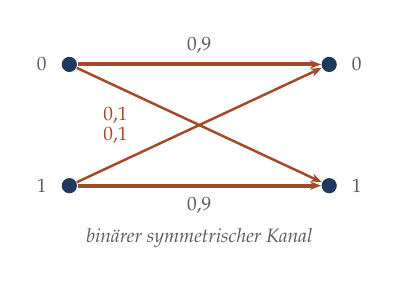
\begin{tikzpicture}[scale=1.1]
\node[knoten] (x0) at (0,0.7) {}; \node[knoten] (x1) at (0,-0.7) {};
\node[knoten] (y0) at (3.0,0.7) {}; \node[knoten] (y1) at (3.0,-0.7) {};
\draw[kanted, -{Stealth[length=4pt]}] (x0)--(y0) node[midway,above,font=\scriptsize,color=grau] {$0{,}9$};
\draw[kanted, -{Stealth[length=4pt]}] (x1)--(y1) node[midway,below,font=\scriptsize,color=grau] {$0{,}9$};
\draw[kante, akzent, -{Stealth[length=4pt]}] (x0)--(y1) node[pos=0.25,below left,font=\scriptsize,color=akzent] {$0{,}1$};
\draw[kante, akzent, -{Stealth[length=4pt]}] (x1)--(y0) node[pos=0.25,above left,font=\scriptsize,color=akzent] {$0{,}1$};
\node[font=\scriptsize, color=grau, anchor=east] at (-0.15,0.7) {$0$};
\node[font=\scriptsize, color=grau, anchor=east] at (-0.15,-0.7) {$1$};
\node[font=\scriptsize, color=grau, anchor=west] at (3.15,0.7) {$0$};
\node[font=\scriptsize, color=grau, anchor=west] at (3.15,-0.7) {$1$};
\node[font=\scriptsize\itshape, color=grau] at (1.5,-1.3) {binärer symmetrischer Kanal};
\end{tikzpicture}
\end{center}

\textbf{Die Frage:} Wie viel lässt sich je Kanalbenutzung fehlerfrei übertragen?

\begin{center}
\begin{minipage}{0.88\textwidth}
\kursiv{Die naheliegende Antwort lautet: weniger als ein Bit, und zwar umso weniger, je fehlerfreier man es haben will. Die richtige Antwort ist $0{,}531$ Bit --- und zwar \kursiv{bei beliebig kleiner Fehlerrate}. Dieses Kapitel erklärt, woher die Zahl kommt; Kapitel~5 beweist, dass sie erreichbar ist.}
\end{minipage}
\end{center}
\end{merksatz}

\section{Transinformation}

\begin{definition}
\boxtitelm{Definition 4.1}
Die \Begriff{Transinformation} zwischen $X$ und $Y$ ist
\[ I(X;Y) = \Ent(X) - \Ent(X\mid Y) . \]
\end{definition}

\begin{merksatz}
\boxtitel{Satz 4.2 --- drei gleichwertige Formen}
\[ I(X;Y) = \Ent(X)-\Ent(X\mid Y) = \Ent(Y)-\Ent(Y\mid X) = \Ent(X)+\Ent(Y)-\Ent(X,Y) \]

\schritt{Beweis}
Nach der Kettenregel (Satz 2.5) gilt
\[ \Ent(X,Y) = \Ent(Y) + \Ent(X\mid Y) \quad\Longrightarrow\quad \Ent(X\mid Y) = \Ent(X,Y)-\Ent(Y) \]
Einsetzen in Definition 4.1:
\[ I(X;Y) = \Ent(X) - \Ent(X,Y) + \Ent(Y) \]
Das ist die dritte Form. Sie ist in $X$ und $Y$ symmetrisch, also stimmt sie auch mit der zweiten überein. $\blacksquare$

\begin{center}
\begin{minipage}{0.9\textwidth}
\textbf{Die Transinformation ist symmetrisch:} Was $Y$ über $X$ verrät, ist genau so viel wie umgekehrt.
\end{minipage}
\end{center}

\begin{center}
\begin{minipage}{0.88\textwidth}
\kursiv{Das ist keineswegs selbstverständlich. Der Laborwert verrät $0{,}12$ Bit über die Diagnosegruppe, und die Diagnosegruppe genau so viel über den Laborwert --- obwohl beide Größen ganz verschiedene Entropien haben ($0{,}81$ und $0{,}72$ Bit). \textbf{Die Auskunft ist gegenseitig und gleich groß.}}
\end{minipage}
\end{center}
\end{merksatz}

\begin{merksatz}
\boxtitel{Das Bild}
\begin{center}
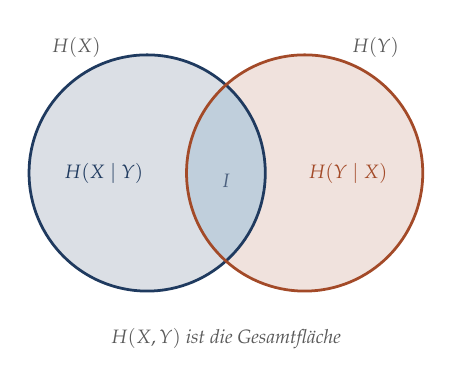
\begin{tikzpicture}[scale=1.0]
\fill[tief!16] (0,0) circle (1.5);
\fill[akzent!16] (2.0,0) circle (1.5);
\begin{scope}
\clip (0,0) circle (1.5);
\fill[mittel!30] (2.0,0) circle (1.5);
\end{scope}
\draw[tief, line width=1.0pt] (0,0) circle (1.5);
\draw[akzent, line width=1.0pt] (2.0,0) circle (1.5);
\node[font=\scriptsize, color=tief] at (-0.55,0) {$\Ent(X\mid Y)$};
\node[font=\scriptsize, color=akzent] at (2.55,0) {$\Ent(Y\mid X)$};
\node[font=\scriptsize, color=tief!80] at (1.0,-0.1) {$I$};
\node[font=\scriptsize, color=grau] at (-0.9,1.6) {$\Ent(X)$};
\node[font=\scriptsize, color=grau] at (2.9,1.6) {$\Ent(Y)$};
\node[font=\scriptsize\itshape, color=grau] at (1.0,-2.1) {$\Ent(X,Y)$ ist die Gesamtfläche};
\end{tikzpicture}
\end{center}

\begin{center}
\begin{minipage}{0.88\textwidth}
\kursiv{Das Bild ist eine nützliche Merkhilfe und hat eine Grenze: Bei drei Größen kann der \enquote{Schnitt aller drei} negativ werden. Die Mengenanalogie trägt also nur bis zu zwei Größen; darüber hinaus muss man rechnen.}
\end{minipage}
\end{center}
\end{merksatz}

\section{Die relative Entropie}

\begin{definition}
\boxtitelm{Definition 4.3}
Für zwei Verteilungen $p$ und $q$ über derselben Menge ist die \Begriff{relative Entropie}
\[ D(p\,\|\,q) = \sum_i p_i\,\lb\frac{p_i}{q_i} . \]
\end{definition}

\begin{merksatz}
\boxtitel{Satz 4.4 --- sie ist nichtnegativ}
\[ D(p\,\|\,q) \ \ge\ 0 , \]
mit Gleichheit genau dann, wenn $p = q$.

\schritt{Beweis}
\begin{align*}
-D(p\,\|\,q) &= \sum_i p_i\,\lb\frac{q_i}{p_i}\\
&\le \lb\left(\sum_i p_i\cdot\frac{q_i}{p_i}\right) && \text{(Jensen, $\lb$ konkav)}\\
&= \lb\left(\sum_i q_i\right) = \lb 1 = 0
\end{align*}

Gleichheit gilt wegen der strengen Konkavität genau dann, wenn alle $\frac{q_i}{p_i}$ übereinstimmen --- und da beide Summen eins ergeben, bedeutet das $p_i = q_i$. $\blacksquare$

\begin{center}
\begin{minipage}{0.88\textwidth}
\kursiv{Dieser Beweis ist zum dritten Mal derselbe --- nach Satz 2.2 und Satz 3.2. Tatsächlich sind beide Sonderfälle: Satz 2.2 ist $D(p\,\|\,\text{gleichverteilt}) \ge 0$, Satz 3.2 ist $D(p\,\|\,q) \ge 0$ mit $q_i = 2^{-l_i}$. \textbf{Die relative Entropie ist das gemeinsame Werkzeug hinter allen Ungleichungen dieses Bandes.}}
\end{minipage}
\end{center}
\end{merksatz}

\begin{merksatz}
\boxtitel{Satz 4.5 --- Transinformation ist nichtnegativ}
\[ I(X;Y) = D\bigl(p(x,y)\,\|\,p(x)p(y)\bigr) \ \ge\ 0 \]
mit Gleichheit genau bei Unabhängigkeit.

\schritt{Beweis der ersten Gleichung}
\begin{align*}
D\bigl(p(x,y)\,\|\,p(x)p(y)\bigr) &= \sum_{x,y} p(x,y)\,\lb\frac{p(x,y)}{p(x)p(y)}\\
&= \sum_{x,y} p(x,y)\,\lb p(x,y) - \sum_{x,y}p(x,y)\,\lb p(x) - \sum_{x,y}p(x,y)\,\lb p(y)\\
&= -\Ent(X,Y) + \Ent(X) + \Ent(Y)
\end{align*}
Das ist die dritte Form aus Satz 4.2. \checkmark

\schritt{Der Rest}
Folgt aus Satz 4.4. Gleichheit bedeutet $p(x,y) = p(x)p(y)$ --- also Unabhängigkeit. $\blacksquare$

\begin{center}
\begin{minipage}{0.9\textwidth}
\textbf{Damit ist auch Satz 2.6 bewiesen:} Aus $I \ge 0$ und $I = \Ent(Y)-\Ent(Y\mid X)$ folgt $\Ent(Y\mid X) \le \Ent(Y)$.
\end{minipage}
\end{center}

\begin{center}
\begin{minipage}{0.88\textwidth}
\kursiv{Die Transinformation misst also, \kursiv{wie weit} zwei Größen von der Unabhängigkeit entfernt sind --- gemessen als relative Entropie zwischen der tatsächlichen Verbundverteilung und derjenigen, die bei Unabhängigkeit vorläge. Das ist ein Abhängigkeitsmaß, das im Gegensatz zur Korrelation aus Band 17 auch nichtlineare Zusammenhänge erfasst.}
\end{minipage}
\end{center}
\end{merksatz}

\section{Die Kanalkapazität}

\begin{definition}
\boxtitelm{Definition 4.6}
Ein \Begriff{diskreter gedächtnisloser Kanal} ist gegeben durch die Übergangswahrscheinlichkeiten $p(y\mid x)$. Seine \Begriff{Kapazität} ist
\[ C = \max_{p(x)} \ I(X;Y) . \]
\end{definition}

\begin{merksatz}
\boxtitel{Was das Maximum bedeutet}
\begin{center}
{\small
\renewcommand{\arraystretch}{1.52}
\begin{tabular}{@{}P{2.4cm}P{6.2cm}@{}}
\toprule
\textbf{Fest} & Der Kanal, also $p(y\mid x)$ --- den kann man nicht ändern.\\
\textbf{Wählbar} & Die Eingangsverteilung $p(x)$ --- über sie verfügt der Sender.\\
\textbf{Gesucht} & Die beste Wahl und der dabei erreichte Wert.\\
\bottomrule
\end{tabular}}
\end{center}

\begin{center}
\begin{minipage}{0.88\textwidth}
\kursiv{Die Kapazität ist eine Eigenschaft des Kanals allein. Sie sagt zunächst nur, wie viel Information im besten Fall je Benutzung hindurchkommt. Dass sie zugleich die Grenze für \kursiv{fehlerfreie} Übertragung ist, behauptet erst Kapitel~5 --- und das ist der eigentliche Satz.}
\end{minipage}
\end{center}
\end{merksatz}

\begin{merksatz}
\boxtitel{Satz 4.7 --- die Kapazität des binären symmetrischen Kanals}
\[ C = 1 - h(f) \]
mit $h$ als binärer Entropiefunktion, erreicht bei gleichverteiltem Eingang.

\schritt{Beweis --- Schritt 1: die bedingte Entropie}
Ist $X=0$, so ist $Y$ mit Wahrscheinlichkeit $f$ gleich $1$:
\[ \Ent(Y\mid X=0) = h(f) \]
Ebenso $\Ent(Y\mid X=1) = h(f)$.

\[ \Ent(Y\mid X) = p(0)\,h(f) + p(1)\,h(f) = h(f) \]

\begin{center}
\begin{minipage}{0.9\textwidth}
\textbf{$\Ent(Y\mid X)$ hängt nicht von der Eingangsverteilung ab.} Das ist die Besonderheit symmetrischer Kanäle und macht die Rechnung kurz.
\end{minipage}
\end{center}

\schritt{Schritt 2 --- maximieren}
\[ I(X;Y) = \Ent(Y) - \Ent(Y\mid X) = \Ent(Y) - h(f) \]

Da nur $\Ent(Y)$ von $p(x)$ abhängt, ist $\Ent(Y)$ zu maximieren. Nach Satz 2.2 ist $\Ent(Y) \le 1$, mit Gleichheit bei $p(Y=0)=\frac12$.

\schritt{Schritt 3 --- das wird erreicht}
Bei $p(X=0)=\frac12$ gilt
\[ p(Y=0) = \tfrac12(1-f) + \tfrac12 f = \tfrac12 \quad \checkmark \]

Also $C = 1-h(f)$. $\blacksquare$
\end{merksatz}

\begin{merksatz}
\boxtitel{Die Werte}
\begin{center}
{\small
\renewcommand{\arraystretch}{1.48}
\begin{tabular}{@{}P{1.4cm}P{1.8cm}P{1.8cm}P{2.4cm}@{}}
\toprule
$f$ & $h(f)$ & $C$ & \\
\midrule
$0{,}00$ & $0{,}0000$ & $1{,}0000$ & ungestört\\
$0{,}01$ & $0{,}0808$ & $0{,}9192$ & \\
$0{,}05$ & $0{,}2864$ & $0{,}7136$ & \\
$\mathbf{0{,}10}$ & $0{,}4690$ & $\mathbf{0{,}5310}$ & \textcolor{akzent}{Leitfall}\\
$0{,}25$ & $0{,}8113$ & $0{,}1887$ & \\
$0{,}50$ & $1{,}0000$ & $\mathbf{0{,}0000}$ & \textcolor{akzent}{wertlos}\\
$0{,}90$ & $0{,}4690$ & $0{,}5310$ & \\
$1{,}00$ & $0{,}0000$ & $1{,}0000$ & \\
\bottomrule
\end{tabular}}
\end{center}

\schritt{Die beiden bemerkenswerten Zeilen}
\begin{center}
\begin{minipage}{0.9\textwidth}
\textbf{Bei $f=\frac12$ ist die Kapazität null.} Der Ausgang ist dann von der Eingabe unabhängig --- ein reiner Münzwurf.
\end{minipage}
\end{center}

\begin{center}
\begin{minipage}{0.9\textwidth}
\textbf{Bei $f=1$ ist sie wieder eins.} Ein Kanal, der \kursiv{jedes} Bit umkehrt, überträgt vollständig --- man muss nur umdrehen.
\end{minipage}
\end{center}

\begin{center}
\begin{minipage}{0.88\textwidth}
\kursiv{Die Kurve ist symmetrisch um $f=\frac12$, und dort liegt der einzige wertlose Fall. \textbf{Nicht die Stärke der Störung ist entscheidend, sondern ihre Berechenbarkeit.} Eine Störung, die immer zuschlägt, ist keine.}
\end{minipage}
\end{center}

\schritt{Der Leitfall}
Bei $f=0{,}1$ beträgt die Kapazität $0{,}531$ Bit je Kanalbenutzung. Bei $10\,000$ Übertragungen je Sekunde sind das
\[ 5310 \ \text{Bit je Sekunde} \]
--- fehlerfrei, mit geeigneter Codierung.
\end{merksatz}

\section{Andere Kanäle}

\begin{merksatz}
\boxtitel{Der Auslöschungskanal}
Hier geht ein Bit mit Wahrscheinlichkeit $e$ verloren --- der Empfänger erhält ein drittes Zeichen \enquote{unbekannt}, aber nie ein falsches.

\begin{center}
\begin{minipage}{0.9\textwidth}
\[ C = 1 - e \]
\end{minipage}
\end{center}

\schritt{Warum das anschaulich ist}
Ein Anteil $e$ der Bits geht verloren, der Rest kommt unversehrt an.

\begin{center}
\begin{minipage}{0.88\textwidth}
\kursiv{Der Vergleich ist lehrreich: Bei $e=0{,}1$ ist $C = 0{,}9$, bei $f=0{,}1$ nur $0{,}531$. \textbf{Ein Fehler, von dem man weiß, dass er aufgetreten ist, kostet erheblich weniger als einer, den man nicht bemerkt.} Deshalb bauen viele Systeme absichtlich eine Erkennung ein und behandeln erkannte Fehler als Auslöschungen.}
\end{minipage}
\end{center}
\end{merksatz}

\begin{merksatz}
\boxtitel{Der Z-Kanal}
Eine Null kommt sicher an, eine Eins kippt mit Wahrscheinlichkeit $f$ --- etwa bei einem Sensor, der Signale übersehen, aber nicht erfinden kann.

\begin{center}
{\small
\renewcommand{\arraystretch}{1.48}
\begin{tabular}{@{}P{1.6cm}P{2.0cm}P{2.6cm}@{}}
\toprule
$f$ & $C$ & \textbf{bestes $p(1)$}\\
\midrule
$0{,}1$ & $0{,}763$ & $0{,}456$\\
$0{,}5$ & $0{,}322$ & $0{,}400$\\
\bottomrule
\end{tabular}}
\end{center}

\begin{center}
\begin{minipage}{0.9\textwidth}
\textbf{Die beste Eingangsverteilung ist nicht gleichverteilt.} Man sendet die störanfällige Eins etwas seltener.
\end{minipage}
\end{center}

\begin{center}
\begin{minipage}{0.88\textwidth}
\kursiv{Und der Vergleich zum symmetrischen Kanal überrascht: Bei $f=0{,}5$ hat der Z-Kanal noch $0{,}32$ Bit Kapazität, der symmetrische null. Obwohl die Hälfte der Einsen verlorengeht, bleibt Information übrig --- weil eine empfangene Eins \kursiv{sicher} eine gesendete Eins war. \textbf{Asymmetrie ist ein Vorteil.}}
\end{minipage}
\end{center}
\end{merksatz}

\section{Der Bruchfall}

\begin{warnung}
\boxtitelr{Was Definition 4.6 voraussetzt}
\begin{center}
{\small
\renewcommand{\arraystretch}{1.52}
\begin{tabular}{@{}P{2.4cm}P{6.2cm}@{}}
\toprule
\textbf{Gedächtnislos} & Jede Benutzung stört unabhängig. Tatsächliche Funkstrecken haben Schwundlöcher --- Fehler treten gebündelt auf.\\
\textbf{Bekannt} & Die Übergangswahrscheinlichkeiten müssen bekannt sein. Sie schwanken mit Wetter, Entfernung und Störquellen.\\
\textbf{Diskret} & Reale Kanäle sind stetig; die Diskretisierung ist selbst eine Modellentscheidung.\\
\bottomrule
\end{tabular}}
\end{center}

\schritt{Zur ersten Zeile}
Bei gebündelten Fehlern ist die Kapazität \kursiv{höher} als beim gedächtnislosen Kanal gleicher mittlerer Fehlerrate --- die Bündelung ist zusätzliche Struktur, die man ausnutzen kann.

\begin{center}
\begin{minipage}{0.88\textwidth}
\kursiv{Praktisch nutzt man das durch \Begriff{Verschachtelung}: Man verteilt die Bits eines Codeworts über einen längeren Zeitraum, so dass ein Schwundloch viele Codewörter leicht statt eines schwer trifft. Das ist eine Anpassung des Systems an den Kanal, nicht umgekehrt.}
\end{minipage}
\end{center}

\schritt{Zur dritten Zeile}
Für den stetigen Kanal mit Gaußschem Rauschen gilt
\[ C = \tfrac12\,\lb\!\left(1+\frac{S}{N}\right) \ \text{Bit je Benutzung} \]
mit dem Verhältnis $S/N$ von Signal- zu Rauschleistung.

\begin{center}
\begin{minipage}{0.88\textwidth}
\kursiv{Das ist die berühmteste Formel der Nachrichtentechnik. Sie besagt, dass die Kapazität nur \kursiv{logarithmisch} mit der Sendeleistung wächst: Eine Verdopplung der Leistung bringt bei gutem Empfang etwa ein halbes Bit. Wer die Datenrate verdoppeln will, braucht bei hohem $S/N$ die quadrierte Leistung --- oder mehr Bandbreite.}
\end{minipage}
\end{center}
\end{warnung}

\begin{warnung}
\boxtitelr{Und die Kapazität ist noch keine Aussage über Codes}
\begin{center}
\begin{minipage}{0.9\textwidth}
\textbf{Definition 4.6 definiert ein Maximum von Transinformation. Dass dieses Maximum die Grenze fehlerfreier Übertragung ist, steht dort nicht.}
\end{minipage}
\end{center}

\begin{center}
\begin{minipage}{0.88\textwidth}
\kursiv{Beide Richtungen sind eigene Sätze. Dass man nicht mehr übertragen kann, folgt aus der Datenverarbeitungsungleichung; dass man so viel erreichen \kursiv{kann}, war Shannons eigentliche Leistung --- und sein Beweis ist nicht konstruktiv. Kapitel~5 behandelt beides.}
\end{minipage}
\end{center}
\end{warnung}

\section{Übungsaufgaben}

\begin{aufgabe}
\boxtitel{Aufgabe 4.1 --- Transinformation berechnen}
Für die Verbundverteilung aus Kapitel~2
\begin{center}
{\small
\renewcommand{\arraystretch}{1.44}
\begin{tabular}{@{}P{2.0cm}P{1.8cm}P{1.8cm}@{}}
\toprule
& $Y=+$ & $Y=-$\\
\midrule
$X=A$ & $0{,}125$ & $0{,}125$\\
$X=\bar A$ & $0{,}075$ & $0{,}675$\\
\bottomrule
\end{tabular}}
\end{center}
berechnen Sie $I(X;Y)$ auf drei Wegen.

\loesung
\schritt{Weg 1 --- über $\Ent(Y)-\Ent(Y\mid X)$}
Aus Kapitel~2: $\Ent(Y) = 0{,}7219$, $\Ent(Y\mid X) = 0{,}6017$.
\[ I = 0{,}7219 - 0{,}6017 = \mathbf{0{,}1202} \]

\schritt{Weg 2 --- über $\Ent(X)-\Ent(X\mid Y)$}
$\Ent(X) = 0{,}8113$, $\Ent(X\mid Y) = \Ent(X,Y)-\Ent(Y) = 1{,}4130-0{,}7219 = 0{,}6911$.
\[ I = 0{,}8113 - 0{,}6911 = \mathbf{0{,}1202} \quad \checkmark \]

\schritt{Weg 3 --- über die relative Entropie}
\[ I = \sum_{x,y} p(x,y)\,\lb\frac{p(x,y)}{p(x)p(y)} \]

\begin{center}
{\small
\renewcommand{\arraystretch}{1.48}
\begin{tabular}{@{}P{1.6cm}P{1.6cm}P{1.8cm}P{1.6cm}P{1.8cm}@{}}
\toprule
$(x,y)$ & $p(x,y)$ & $p(x)p(y)$ & \textbf{Quotient} & \textbf{Beitrag}\\
\midrule
$(A,+)$ & $0{,}125$ & $0{,}050$ & $2{,}500$ & $0{,}1653$\\
$(A,-)$ & $0{,}125$ & $0{,}200$ & $0{,}625$ & $-0{,}0848$\\
$(\bar A,+)$ & $0{,}075$ & $0{,}150$ & $0{,}500$ & $-0{,}0750$\\
$(\bar A,-)$ & $0{,}675$ & $0{,}600$ & $1{,}125$ & $0{,}1147$\\
\midrule
& & & & $\mathbf{0{,}1202}$\\
\bottomrule
\end{tabular}}
\end{center}

\kursiv{Zum ersten Beitrag:} $0{,}125\cdot\lb 2{,}5 = 0{,}125\cdot1{,}3219 = 0{,}1653$.\\
\kursiv{Zum zweiten:} $0{,}125\cdot\lb0{,}625 = 0{,}125\cdot(-0{,}6781) = -0{,}0848$.

\begin{center}
\begin{minipage}{0.9\textwidth}
\textbf{Beachten Sie die negativen Beiträge.} Die Transinformation ist als Ganzes nichtnegativ; einzelne Summanden können sehr wohl negativ sein.
\end{minipage}
\end{center}

\schritt{Schritt 4 --- Die Deutung}
\begin{center}
\renewcommand{\arraystretch}{1.48}
\begin{tabular}{@{}P{2.8cm}P{2.4cm}P{2.4cm}@{}}
\toprule
& \textbf{Bit} & \textbf{Anteil}\\
\midrule
$\Ent(X)$ & $0{,}8113$ & $100\,\%$\\
davon $I$ & $0{,}1202$ & $14{,}8\,\%$\\
\bottomrule
\end{tabular}
\end{center}

\begin{center}
\begin{minipage}{0.88\textwidth}
\kursiv{Der Laborwert nimmt knapp fünfzehn Prozent der Ungewissheit über die Diagnosegruppe. Das ist ein brauchbarer, aber kein durchschlagender Befund --- und die Zahl ist eine sinnvolle Kenngröße für die Güte eines diagnostischen Tests, die neben Empfindlichkeit und Trennschärfe aus Band 17 tritt.}
\end{minipage}
\end{center}
\end{aufgabe}

\begin{aufgabe}
\boxtitel{Aufgabe 4.2 --- Kapazitäten vergleichen}
Bestimmen Sie die Kapazität:
\begin{center}
{\small
\renewcommand{\arraystretch}{1.4}
\begin{tabular}{@{}P{0.8cm}P{7.6cm}@{}}
\toprule
(a) & Binärer symmetrischer Kanal mit $f=0{,}05$.\\
(b) & Auslöschungskanal mit $e=0{,}05$.\\
(c) & Zwei unabhängige Kanäle nach (a) nebeneinander.\\
(d) & Ein Kanal nach (a), zweimal hintereinander durchlaufen.\\
\bottomrule
\end{tabular}}
\end{center}

\loesung
\schritt{(a)}
\[ h(0{,}05) = -0{,}05\,\lb0{,}05 - 0{,}95\,\lb0{,}95 \]
\[ = 0{,}05\cdot4{,}3219 + 0{,}95\cdot0{,}0740 = 0{,}2161+0{,}0703 = 0{,}2864 \]
\[ C = 1-0{,}2864 = \mathbf{0{,}7136} \]

\schritt{(b)}
\[ C = 1-0{,}05 = \mathbf{0{,}9500} \]

\kursiv{Vergleich:} Derselbe Störanteil kostet beim Auslöschungskanal $0{,}05$ Bit, beim symmetrischen $0{,}29$ --- fast das Sechsfache.

\schritt{(c) Zwei parallele Kanäle}
Die Kapazitäten addieren sich:
\[ C = 2\cdot0{,}7136 = \mathbf{1{,}4272} \]

\kursiv{Begründung:} Die beiden Kanäle stören unabhängig, also ist die Transinformation des Paares die Summe.

\schritt{(d) Zwei Kanäle hintereinander}
Ein Bit kommt genau dann richtig an, wenn es entweder zweimal richtig oder zweimal falsch übertragen wurde:
\[ f_{\text{ges}} = 2\cdot0{,}05\cdot0{,}95 = 0{,}095 \]

\[ h(0{,}095) = 0{,}095\cdot3{,}3959 + 0{,}905\cdot0{,}1440 = 0{,}3226+0{,}1303 = 0{,}4529 \]
\[ C = 1-0{,}4529 = \mathbf{0{,}5471} \]

\schritt{Die Übersicht}
\begin{center}
{\small
\renewcommand{\arraystretch}{1.48}
\begin{tabular}{@{}P{2.4cm}P{2.2cm}P{3.0cm}@{}}
\toprule
& $C$ & \\
\midrule
(a) einfach & $0{,}7136$ & \\
(b) Auslöschung & $0{,}9500$ & \textcolor{gruen}{erkennbare Fehler}\\
(c) parallel & $1{,}4272$ & doppelt\\
(d) hintereinander & $0{,}5471$ & \textcolor{akzent}{weniger als (a)}\\
\bottomrule
\end{tabular}}
\end{center}

\begin{center}
\begin{minipage}{0.9\textwidth}
\textbf{Hintereinandergeschaltete Kanäle können nur verlieren.}
\end{minipage}
\end{center}

\begin{center}
\begin{minipage}{0.88\textwidth}
\kursiv{Das ist ein Sonderfall der \Begriff{Datenverarbeitungsungleichung}: Bilden $X \to Y \to Z$ eine Kette, in der $Z$ nur über $Y$ von $X$ abhängt, so gilt $I(X;Z) \le I(X;Y)$. \textbf{Keine Nachbearbeitung kann Information hinzufügen, die nicht angekommen ist.} Kapitel~5 beweist die Ungleichung und benutzt sie für die Umkehrung des Codierungstheorems.}
\end{minipage}
\end{center}
\end{aufgabe}

\begin{aufgabe}
\boxtitel{Aufgabe 4.3 --- Der Wiederholungscode}
Beim Leitfall ($f=0{,}1$) wird jedes Bit $n$-mal gesendet; der Empfänger entscheidet nach Mehrheit. Bestimmen Sie Rate und Fehlerwahrscheinlichkeit und vergleichen Sie mit der Kapazität.

\loesung
\schritt{Schritt 1 --- Die Fehlerwahrscheinlichkeit}
Ein Fehler tritt auf, wenn mehr als die Hälfte der Bits kippt:
\[ P_e = \sum_{i=\lceil n/2\rceil}^{n} \binom{n}{i}\,f^{i}\,(1-f)^{\,n-i} \]

\schritt{Schritt 2 --- Für $n=3$}
\[ P_e = \binom32 (0{,}1)^2(0{,}9) + \binom33 (0{,}1)^3 = 3\cdot0{,}009 + 0{,}001 = 0{,}028 \]

\schritt{Schritt 3 --- Für $n=5$}
\[ P_e = 10\,(0{,}1)^3(0{,}9)^2 + 5\,(0{,}1)^4(0{,}9) + (0{,}1)^5 \]
\[ = 10\cdot0{,}00081 + 5\cdot0{,}00009 + 0{,}00001 = 0{,}0081+0{,}00045+0{,}00001 = 0{,}00856 \]

\schritt{Schritt 4 --- Die Tabelle}
\begin{center}
{\small
\renewcommand{\arraystretch}{1.48}
\begin{tabular}{@{}P{1.4cm}P{2.0cm}P{2.4cm}@{}}
\toprule
$n$ & \textbf{Rate} & $P_e$\\
\midrule
$1$ & $1{,}0000$ & $1{,}0\cdot10^{-1}$\\
$3$ & $0{,}3333$ & $2{,}8\cdot10^{-2}$\\
$5$ & $0{,}2000$ & $8{,}6\cdot10^{-3}$\\
$9$ & $0{,}1111$ & $8{,}9\cdot10^{-4}$\\
$11$ & $0{,}0909$ & $3{,}0\cdot10^{-4}$\\
$21$ & $0{,}0476$ & $1{,}4\cdot10^{-6}$\\
\bottomrule
\end{tabular}}
\end{center}

\schritt{Schritt 5 --- Der Befund}
\begin{center}
\begin{minipage}{0.9\textwidth}
\textbf{Um die Fehlerrate zu senken, muss die Rate gesenkt werden --- und für $P_e \to 0$ geht sie gegen null.}
\end{minipage}
\end{center}

\schritt{Schritt 6 --- Der Vergleich mit der Kapazität}
\[ C = 1-h(0{,}1) = 0{,}5310 \]

\begin{center}
\renewcommand{\arraystretch}{1.48}
\begin{tabular}{@{}P{2.8cm}P{2.2cm}P{2.4cm}@{}}
\toprule
& \textbf{Rate} & $P_e$\\
\midrule
Wiederholung, $n=21$ & $0{,}048$ & $1{,}4\cdot10^{-6}$\\
\textbf{Shannon} & $\mathbf{0{,}531}$ & \textbf{beliebig klein}\\
\bottomrule
\end{tabular}
\end{center}

\begin{center}
\begin{minipage}{0.9\textwidth}
\textbf{Die Kapazität liegt beim Elffachen dessen, was der Wiederholungscode bei dieser Fehlerrate schafft.}
\end{minipage}
\end{center}

\schritt{Schritt 7 --- Warum Wiederholung so schlecht ist}
\begin{center}
\begin{minipage}{0.88\textwidth}
\kursiv{Der Wiederholungscode schützt jedes Bit einzeln. Ein guter Code schützt einen ganzen Block \kursiv{gemeinsam} --- und nutzt dabei aus, dass die Zahl der möglichen Fehlermuster viel kleiner ist als die Zahl der möglichen Blöcke. Bei einem Block von $100$ Bit und $f=0{,}1$ sind typischerweise etwa zehn Bit falsch. Die Zahl der Fehlermuster mit \kursiv{höchstens} zehn falschen Bit beträgt rund $2^{47}$ --- gegenüber $2^{100}$ Blöcken.}
\end{minipage}
\end{center}

\begin{center}
\begin{minipage}{0.88\textwidth}
\kursiv{Genauer: $100\cdot h(0{,}1) = 46{,}9$, und das ist der Logarithmus der Zahl typischer Fehlermuster. Von den hundert Bit gehen also $46{,}9$ an die Störung verloren, und $53{,}1$ bleiben nutzbar --- genau $100\cdot C$. \textbf{Das ist der ganze Gedanke des nächsten Kapitels, an einer einzigen Zahl abgelesen.}}
\end{minipage}
\end{center}
\end{aufgabe}

\begin{geschichte}
\boxtitelg{Eine Zahl, die niemand erwartet hatte}
Vor 1948 galt als ausgemacht, dass Störungen nur durch Wiederholung zu bekämpfen sind --- und dass fehlerfreie Übertragung deshalb unendlich langsam werden muss.

\begin{center}
\begin{minipage}{0.9\textwidth}
\kursiv{Die Rechnung aus Aufgabe 4.3 war bekannt und schien die Sache zu entscheiden: Die Fehlerrate fällt exponentiell, die Rate aber wie $1/n$. Für beliebig kleine Fehler muss man beliebig langsam werden.}
\end{minipage}
\end{center}

\schritt{Der Bruch}
Shannon zeigte, dass diese Schlussfolgerung nur für \kursiv{Wiederholungscodes} gilt --- und dass es bessere gibt.

\begin{center}
\begin{minipage}{0.9\textwidth}
\kursiv{Zeitgenossen berichteten, das Ergebnis sei zunächst auf Unglauben gestoßen. Es widerspricht nicht nur der Anschauung, sondern auch der Erfahrung jedes Nachrichtentechnikers. \Person{Robert Fano} sagte später, er habe nicht geglaubt, dass so etwas möglich sei, bis er den Beweis mehrfach durchgegangen sei.}
\end{minipage}
\end{center}

\schritt{Die Vorgeschichte der Größe}
Der Begriff der Kanalkapazität stammt in Ansätzen von \Person{Nyquist} (1924), der die höchste Symbolrate bei gegebener Bandbreite bestimmte, und von \Person{Hartley} (1928).

\begin{center}
\begin{minipage}{0.9\textwidth}
\kursiv{Beiden fehlte die Behandlung des Rauschens. Shannons Beitrag war, Störungen nicht als technischen Mangel zu behandeln, sondern als wahrscheinlichkeitstheoretisches Objekt --- und damit dieselbe Größe darauf anzuwenden, die er für Quellen entwickelt hatte.}
\end{minipage}
\end{center}

\schritt{Die relative Entropie}
\Person{Solomon Kullback} und \Person{Richard Leibler} führten sie 1951 ein, als Maß für die Unterscheidbarkeit zweier Verteilungen.

\begin{center}
\begin{minipage}{0.9\textwidth}
\kursiv{Kullback arbeitete zu dieser Zeit für den amerikanischen Nachrichtendienst und hatte während des Krieges an der Entzifferung japanischer Chiffren mitgewirkt. Die Größe, die heute in der Statistik und im maschinellen Lernen allgegenwärtig ist, entstand aus der Frage, wie gut sich zwei Hypothesen anhand abgefangener Nachrichten trennen lassen.}
\end{minipage}
\end{center}
\end{geschichte}

\begin{forschung}
\boxtitelp{Kapazität in der Praxis}
\begin{center}
{\small
\renewcommand{\arraystretch}{1.45}
\begin{tabular}{@{}P{2.8cm}P{5.4cm}@{}}
\toprule
\textbf{Mehrantennen\-systeme} & Mehrere Sende- und Empfangsantennen erzeugen mehrere parallele Kanäle; die Kapazität wächst näherungsweise linear mit ihrer Zahl.\\
\textbf{Netzwerke} & Für Kanäle mit mehreren Sendern und Empfängern ist die Kapazität in vielen Fällen bis heute unbekannt.\\
\textbf{Rückkanal} & Eine Rückmeldung erhöht die Kapazität des gedächtnislosen Kanals \kursiv{nicht} --- sie vereinfacht aber die Codes erheblich.\\
\bottomrule
\end{tabular}}
\end{center}

\schritt{Zur zweiten Zeile}
Schon der einfachste Fall --- zwei Sender, ein Empfänger, ein Störkanal --- ist ungelöst.

\begin{center}
\begin{minipage}{0.88\textwidth}
\kursiv{Für den \Begriff{Interferenzkanal} mit zwei Sender-Empfänger-Paaren ist die Kapazität seit den 1970er Jahren offen; man kennt Schranken, die sich um höchstens ein Bit unterscheiden --- ein Ergebnis von 2008, das als Durchbruch galt. \textbf{Die Informationstheorie ist bei einem Sender vollständig und bei mehreren weitgehend offen.}}
\end{minipage}
\end{center}

\schritt{Zur dritten Zeile}
Dass Rückmeldung die Kapazität nicht erhöht, ist ein Satz von Shannon.

\begin{center}
\begin{minipage}{0.88\textwidth}
\kursiv{Das überrascht, weil ein Rückkanal offensichtlich nützlich ist --- man kann verlorene Blöcke nachfordern. Der Satz besagt, dass dieser Nutzen in der \kursiv{Einfachheit} liegt, nicht in der erreichbaren Rate. Bei Kanälen mit Gedächtnis gilt er allerdings nicht mehr.}
\end{minipage}
\end{center}
\end{forschung}

\begin{merksatz}
\boxtitel{Was Sie jetzt können}
\begin{center}
\renewcommand{\arraystretch}{1.5}
\begin{tabular}{@{}P{3.0cm}P{5.6cm}@{}}
\toprule
\textbf{Satz 4.2} & drei Formen, Symmetrie\\
\textbf{Satz 4.4} & $D(p\|q)\ge0$ --- das gemeinsame Werkzeug\\
\textbf{Satz 4.5} & $I \ge 0$, null bei Unabhängigkeit\\
\textbf{Definition 4.6} & $C = \max_{p(x)} I(X;Y)$\\
\textbf{Satz 4.7} & $C = 1-h(f)$ beim BSC\\
\bottomrule
\end{tabular}
\end{center}

\begin{center}
\begin{minipage}{0.88\textwidth}
\kursiv{Im nächsten Kapitel wird aus der Zahl $0{,}531$ ein Satz --- und zwar der überraschendste dieses Bandes.}
\end{minipage}
\end{center}
\end{merksatz}

\chapter{Das Kanalcodierungstheorem}

\section{Die Aussage}

\begin{merksatz}
\boxtitel{Satz 5.1 --- Shannon, 1948}
Sei $C$ die Kapazität eines diskreten gedächtnislosen Kanals.

\begin{center}
{\small
\renewcommand{\arraystretch}{1.55}
\begin{tabular}{@{}P{2.0cm}P{6.6cm}@{}}
\toprule
\textbf{Erreichbar} & Für jede Rate $R < C$ und jedes $\varepsilon > 0$ gibt es ein $n$ und einen Code der Länge $n$ mit Rate $R$, dessen Fehlerwahrscheinlichkeit kleiner als $\varepsilon$ ist.\\
\textbf{Umkehrung} & Für $R > C$ lässt sich die Fehlerwahrscheinlichkeit nicht beliebig klein machen.\\
\bottomrule
\end{tabular}}
\end{center}

\begin{center}
\begin{minipage}{0.9\textwidth}
\textbf{Der Übergang bei $R = C$ ist scharf.} Unterhalb geht alles, oberhalb nichts.
\end{minipage}
\end{center}

\begin{center}
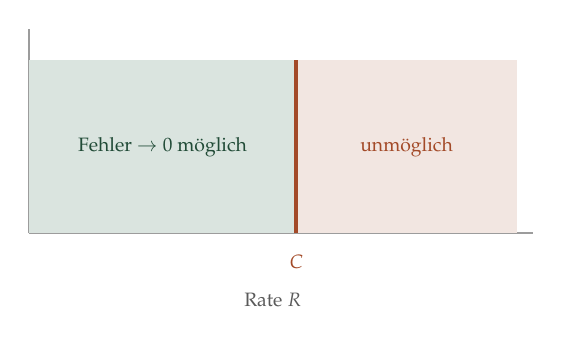
\begin{tikzpicture}[scale=1.0]
\draw[grau!60, line width=0.7pt] (0,0) -- (6.4,0);
\draw[grau!60, line width=0.7pt] (0,0) -- (0,2.6);
\fill[gruen!18] (0,0) rectangle (3.4,2.2);
\fill[akzent!14] (3.4,0) rectangle (6.2,2.2);
\draw[akzent, line width=1.4pt] (3.4,0) -- (3.4,2.2);
\node[font=\scriptsize, color=gruen!70!black] at (1.7,1.1) {Fehler $\to 0$ möglich};
\node[font=\scriptsize, color=akzent] at (4.8,1.1) {unmöglich};
\node[font=\scriptsize, color=akzent, anchor=north] at (3.4,-0.15) {$C$};
\node[font=\scriptsize, color=grau] at (3.1,-0.85) {Rate $R$};
\end{tikzpicture}
\end{center}

\begin{center}
\begin{minipage}{0.88\textwidth}
\kursiv{Beide Teile sind bemerkenswert. Die Umkehrung entspricht der Erwartung --- irgendwo muss eine Grenze liegen. Die Erreichbarkeit widerspricht ihr: Sie behauptet, dass bis unmittelbar an diese Grenze heran \kursiv{beliebig} zuverlässig übertragen werden kann.}
\end{minipage}
\end{center}
\end{merksatz}

\section{Typische Folgen}

\begin{merksatz}
\boxtitel{Der Schlüsselbegriff}
Eine Quelle liefert unabhängige Symbole. Betrachtet man lange Folgen, so zerfällt der Raum aller Folgen in zwei sehr ungleiche Teile.

\schritt{Ein Zahlenbeispiel}
Eine Binärquelle mit $p(1) = 0{,}1$, Folgen der Länge $100$.

\begin{center}
{\small
\renewcommand{\arraystretch}{1.5}
\begin{tabular}{@{}P{2.6cm}P{2.4cm}P{2.6cm}@{}}
\toprule
& \textbf{Anzahl} & \textbf{Gesamt-Wahrsch.}\\
\midrule
Alle Folgen & $2^{100}$ & $1$\\
\textbf{Typische} & $\approx 2^{46{,}9}$ & $\approx 1$\\
\bottomrule
\end{tabular}}
\end{center}

\begin{center}
\begin{minipage}{0.9\textwidth}
\textbf{Ein Anteil von $2^{-53{,}1} \approx 10^{-16}$ aller Folgen trägt nahezu die gesamte Wahrscheinlichkeit.}
\end{minipage}
\end{center}

\begin{center}
\begin{minipage}{0.88\textwidth}
\kursiv{Anschaulich: Fast jede tatsächlich auftretende Folge hat etwa zehn Einsen. Folgen mit fünfzig Einsen gibt es zwar weit mehr, aber sie kommen praktisch nie vor. \textbf{Die Menge der typischen Folgen ist winzig und trägt alles.}}
\end{minipage}
\end{center}
\end{merksatz}

\begin{definition}
\boxtitelm{Definition 5.2 --- typische Menge}
Für $\varepsilon > 0$ ist
\[ A_\varepsilon^{(n)} = \left\{ (x_1,\ldots,x_n) \ : \ \left|-\tfrac1n\,\lb p(x_1,\ldots,x_n) - \Ent(X)\right| \le \varepsilon \right\} . \]
\end{definition}

\begin{merksatz}
\boxtitel{Satz 5.3 --- die asymptotische Gleichverteilungseigenschaft}
\begin{center}
{\small
\renewcommand{\arraystretch}{1.55}
\begin{tabular}{@{}P{1.0cm}P{7.4cm}@{}}
\toprule
$1$ & $\Pr\bigl[A_\varepsilon^{(n)}\bigr] \to 1$ für $n\to\infty$.\\
$2$ & $\bigl|A_\varepsilon^{(n)}\bigr| \le 2^{\,n(\Ent+\varepsilon)}$.\\
$3$ & $\bigl|A_\varepsilon^{(n)}\bigr| \ge (1-\varepsilon)\,2^{\,n(\Ent-\varepsilon)}$ für hinreichend großes $n$.\\
\bottomrule
\end{tabular}}
\end{center}

\schritt{Beweis von 1}
Für unabhängige Symbole gilt
\[ -\frac1n\,\lb p(x_1,\ldots,x_n) = -\frac1n\sum_{i=1}^{n} \lb p(x_i) . \]

Das ist der Mittelwert von $n$ unabhängigen, gleichverteilten Zufallsgrößen $-\lb p(X_i)$ mit dem Erwartungswert
\[ \mathbb{E}\bigl[-\lb p(X)\bigr] = -\sum_x p(x)\,\lb p(x) = \Ent(X) . \]

Nach dem schwachen Gesetz der großen Zahlen (Band 12) strebt dieser Mittelwert in Wahrscheinlichkeit gegen $\Ent(X)$. \checkmark

\schritt{Beweis von 2}
Für jede typische Folge gilt nach Definition
\[ p(x_1,\ldots,x_n) \ \ge\ 2^{-n(\Ent+\varepsilon)} . \]
Da die Gesamtwahrscheinlichkeit höchstens eins ist:
\[ 1 \ \ge\ \sum_{\vek{x}\in A} p(\vek{x}) \ \ge\ \bigl|A\bigr|\cdot 2^{-n(\Ent+\varepsilon)} \]
Umstellen liefert die Behauptung. \checkmark

\schritt{Beweis von 3}
Nach Teil 1 ist $\Pr[A] \ge 1-\varepsilon$ für großes $n$. Andererseits ist jede Einzelwahrscheinlichkeit höchstens $2^{-n(\Ent-\varepsilon)}$:
\[ 1-\varepsilon \ \le\ \Pr[A] \ \le\ |A|\cdot 2^{-n(\Ent-\varepsilon)} \]
$\blacksquare$

\begin{center}
\begin{minipage}{0.88\textwidth}
\kursiv{Der Satz besagt, dass sich die typischen Folgen näherungsweise wie eine \kursiv{Gleichverteilung} über $2^{n\Ent}$ Möglichkeiten verhalten --- daher der Name. Das ist der Grund, warum man in der Informationstheorie so oft mit Zweierpotenzen abzählen darf: Man arbeitet in Wahrheit stets auf der typischen Menge.}
\end{minipage}
\end{center}
\end{merksatz}

\section{Der Beweisgedanke}

\begin{merksatz}
\boxtitel{Die Kugelpackung}
Beim binären symmetrischen Kanal mit Fehlerrate $f$ gilt: Wird $\vek{x}$ gesendet, so ist das Rauschmuster typisch --- es enthält etwa $nf$ Einsen.

\begin{center}
\begin{minipage}{0.9\textwidth}
\textbf{Der Empfangsvektor liegt also in einer \enquote{Kugel} von etwa $2^{\,n\,h(f)}$ Folgen um $\vek{x}$.}
\end{minipage}
\end{center}

\schritt{Die Abzählung}
\begin{center}
{\small
\renewcommand{\arraystretch}{1.5}
\begin{tabular}{@{}P{2.8cm}P{2.6cm}P{2.4cm}@{}}
\toprule
& \textbf{allgemein} & $n=100$, $f=0{,}1$\\
\midrule
Alle Folgen & $2^{n}$ & $2^{100}$\\
Eine Kugel & $2^{\,n\,h(f)}$ & $2^{46{,}9}$\\
\textbf{Kugeln, die passen} & $2^{\,n(1-h(f))}$ & $\mathbf{2^{53{,}1}}$\\
\bottomrule
\end{tabular}}
\end{center}

\[ 1-h(f) = C \]

\begin{center}
\begin{minipage}{0.9\textwidth}
\textbf{Es passen höchstens $2^{nC}$ überschneidungsfreie Kugeln in den Raum --- also höchstens $2^{nC}$ Codewörter.} Das ergibt die Rate $C$.
\end{minipage}
\end{center}

\begin{center}
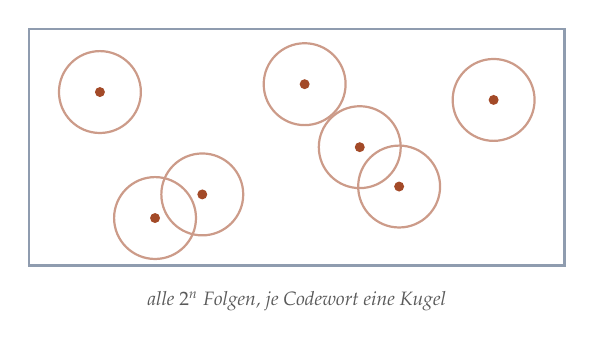
\begin{tikzpicture}[scale=1.0]
\draw[tief!50, line width=1.0pt] (-0.2,-1.5) rectangle (6.6,1.5);
\foreach \x/\y in {0.7/0.7, 2.0/-0.6, 3.3/0.8, 4.5/-0.5, 5.7/0.6, 1.4/-0.9, 4.0/0.0}
  {\draw[akzent!55, line width=0.8pt] (\x,\y) circle (0.52); \fill[akzent] (\x,\y) circle (1.8pt);}
\node[font=\scriptsize\itshape, color=grau] at (3.2,-1.95) {alle $2^{n}$ Folgen, je Codewort eine Kugel};
\end{tikzpicture}
\end{center}

\begin{center}
\begin{minipage}{0.88\textwidth}
\kursiv{Dieses Argument liefert nur die \kursiv{obere} Schranke --- dass nicht mehr geht. Dass so viele Codewörter tatsächlich unterzubringen sind, folgt daraus nicht: Kugelpackungen lassen im Allgemeinen Zwischenräume. Der zweite Teil ist der schwierigere.}
\end{minipage}
\end{center}
\end{merksatz}

\begin{merksatz}
\boxtitel{Die Zufallscodierung}
Shannons Kunstgriff: Statt einen guten Code zu \kursiv{konstruieren}, wählt man ihn zufällig und zeigt, dass er im Mittel gut ist.

\schritt{Der Aufbau}
\begin{center}
\renewcommand{\arraystretch}{1.5}
\begin{tabular}{@{}P{1.0cm}P{7.4cm}@{}}
\toprule
$1$ & Man wähle $2^{\,nR}$ Codewörter der Länge $n$ rein zufällig.\\
$2$ & Sender und Empfänger kennen beide die Tabelle.\\
$3$ & Der Empfänger entscheidet für dasjenige Codewort, das mit dem Empfangenen typisch verbunden ist.\\
\bottomrule
\end{tabular}
\end{center}

\schritt{Die Fehlerabschätzung}
Ein Fehler entsteht, wenn ein \kursiv{falsches} Codewort ebenfalls in die Entscheidungskugel fällt.

\kursiv{Für ein einzelnes falsches Wort:}
\[ \Pr[\text{fällt hinein}] \ \approx\ \frac{2^{\,n\,h(f)}}{2^{n}} = 2^{-n(1-h(f))} = 2^{-nC} \]

\kursiv{Für alle $2^{nR}-1$ falschen zusammen} --- über die Summenabschätzung:
\[ \Pr[\text{Fehler}] \ \lesssim\ 2^{\,nR}\cdot 2^{-nC} = 2^{-n(C-R)} \]

\begin{center}
\begin{minipage}{0.9\textwidth}
\textbf{Für $R < C$ ist der Exponent negativ --- die Fehlerwahrscheinlichkeit fällt exponentiell in $n$.}
\end{minipage}
\end{center}

\schritt{Die Zahlen für den Leitfall}
$f = 0{,}1$, also $C = 0{,}531$:
\begin{center}
{\small
\renewcommand{\arraystretch}{1.48}
\begin{tabular}{@{}P{1.6cm}P{1.4cm}P{2.0cm}P{2.2cm}@{}}
\toprule
$n$ & $R$ & \textbf{Exponent} & \textbf{Schranke}\\
\midrule
$100$ & $0{,}20$ & $-33{,}1$ & $1{,}1\cdot10^{-10}$\\
$100$ & $0{,}40$ & $-13{,}1$ & $1{,}1\cdot10^{-4}$\\
$100$ & $0{,}50$ & $-3{,}1$ & $1{,}2\cdot10^{-1}$\\
$1000$ & $0{,}40$ & $-131$ & $3{,}7\cdot10^{-40}$\\
$1000$ & $0{,}50$ & $-31$ & $4{,}6\cdot10^{-10}$\\
$10\,000$ & $0{,}52$ & $-110$ & $7{,}5\cdot10^{-34}$\\
\bottomrule
\end{tabular}}
\end{center}

\begin{center}
\begin{minipage}{0.88\textwidth}
\kursiv{Die letzte Zeile ist der Punkt: Bei einer Rate von $0{,}52$ --- also $98$ Prozent der Kapazität --- ist die Fehlerwahrscheinlichkeit bei Blocklänge $10\,000$ kleiner als $10^{-33}$. Zum Vergleich: Der Wiederholungscode aus Aufgabe 4.3 erreichte bei Rate $0{,}048$ nur $10^{-6}$.}
\end{minipage}
\end{center}

\schritt{Der letzte Schritt}
Die Rechnung liefert den \kursiv{Mittelwert} über alle zufälligen Codes. Ist der Mittelwert kleiner als $\varepsilon$, so muss mindestens ein Code mindestens so gut sein.

\begin{center}
\begin{minipage}{0.9\textwidth}
\textbf{Also existiert ein guter Code.} Welcher, sagt der Beweis nicht.
\end{minipage}
\end{center}
\end{merksatz}

\section{Die Umkehrung}

\begin{merksatz}
\boxtitel{Satz 5.4 --- die Ungleichung von Fano}
Schätzt man $X$ aus $Y$ mit der Fehlerwahrscheinlichkeit $P_e$, so gilt
\[ \Ent(X\mid Y) \ \le\ h(P_e) + P_e\,\lb\bigl(|\mathcal{X}|-1\bigr) . \]

\schritt{Der Gedanke}
Die verbleibende Ungewissheit zerfällt in zwei Teile: die Frage, \kursiv{ob} ein Fehler vorliegt --- höchstens $h(P_e)$ Bit --- und im Fehlerfall die Frage, welcher der übrigen Werte richtig ist.

\begin{center}
\begin{minipage}{0.9\textwidth}
\textbf{Ist $P_e$ klein, so ist $\Ent(X\mid Y)$ klein.} Das ist die Richtung, die für die Umkehrung gebraucht wird.
\end{minipage}
\end{center}

\begin{center}
{\small
\renewcommand{\arraystretch}{1.46}
\begin{tabular}{@{}P{2.0cm}P{2.6cm}P{2.4cm}@{}}
\toprule
$P_e$ & \textbf{Schranke bei $|\mathcal{X}|=2$} & \\
\midrule
$0{,}001$ & $0{,}0114$ & \\
$0{,}010$ & $0{,}0808$ & \\
$0{,}100$ & $0{,}4690$ & \\
$0{,}500$ & $1{,}0000$ & wertlos\\
\bottomrule
\end{tabular}}
\end{center}
\end{merksatz}

\begin{merksatz}
\boxtitel{Satz 5.5 --- die Datenverarbeitungsungleichung}
Bilden $X \to Y \to Z$ eine Kette --- also hängt $Z$ nur über $Y$ von $X$ ab ---, so gilt
\[ I(X;Z) \ \le\ I(X;Y) . \]

\begin{center}
\begin{minipage}{0.9\textwidth}
\textbf{Keine Nachbearbeitung kann Information hinzufügen, die nicht angekommen ist.}
\end{minipage}
\end{center}

\begin{center}
\begin{minipage}{0.88\textwidth}
\kursiv{Das ist die Aussage hinter Aufgabe 4.2(d), wo zwei hintereinandergeschaltete Kanäle weniger leisteten als einer. Sie hat weitreichende Folgen: \textbf{Kein noch so raffiniertes Verfahren kann aus verrauschten Daten mehr herausholen, als in ihnen steckt} --- eine Warnung, die in der Datenauswertung so oft überhört wird wie in der Nachrichtentechnik.}
\end{minipage}
\end{center}
\end{merksatz}

\begin{merksatz}
\boxtitel{Die Umkehrung des Codierungstheorems}
\schritt{Der Aufbau}
Eine Nachricht $W$ aus $2^{nR}$ Möglichkeiten wird codiert, über den Kanal geschickt und zu $\hat W$ decodiert.

\schritt{Schritt 1 --- die Entropie der Nachricht}
Bei gleichverteilter Nachricht:
\[ \Ent(W) = nR \]

\schritt{Schritt 2 --- zerlegen}
\[ nR = \Ent(W) = I(W;\hat W) + \Ent(W\mid\hat W) \]

\schritt{Schritt 3 --- beide Teile abschätzen}
\begin{center}
\renewcommand{\arraystretch}{1.5}
\begin{tabular}{@{}P{2.6cm}P{6.0cm}@{}}
\toprule
$I(W;\hat W)$ & $\le n\,C$ nach Satz 5.5, da $W \to X^n \to Y^n \to \hat W$\\
$\Ent(W\mid\hat W)$ & $\le 1 + P_e\cdot nR$ nach Satz 5.4\\
\bottomrule
\end{tabular}
\end{center}

\schritt{Schritt 4 --- zusammensetzen}
\[ nR \ \le\ nC + 1 + P_e\,nR \]

Division durch $n$:
\[ R \ \le\ C + \frac1n + P_e\,R \]

\schritt{Schritt 5 --- der Schluss}
Soll $P_e \to 0$ gelten, so folgt im Grenzwert
\[ R \ \le\ C . \]
$\blacksquare$

\begin{center}
\begin{minipage}{0.88\textwidth}
\kursiv{Umgestellt liefert die Ungleichung sogar mehr: $P_e \ge 1 - \frac{C}{R} - \frac{1}{nR}$. \textbf{Oberhalb der Kapazität bleibt die Fehlerwahrscheinlichkeit nicht nur positiv, sondern über einer festen Schranke} --- bei $R = 2C$ etwa über $\frac12$. Es wird also nicht \enquote{ein bisschen schlechter}, sondern unbrauchbar.}
\end{minipage}
\end{center}
\end{merksatz}

\section{Der Bruchfall}

\begin{warnung}
\boxtitelr{Was der Beweis nicht liefert}
\begin{center}
{\small
\renewcommand{\arraystretch}{1.52}
\begin{tabular}{@{}P{2.4cm}P{6.2cm}@{}}
\toprule
\textbf{Keinen Code} & Der Beweis zeigt, dass ein guter Code existiert. Er gibt keinen an.\\
\textbf{Keine Blocklänge} & \enquote{Für hinreichend großes $n$} --- wie groß, steht nicht da.\\
\textbf{Keine Decodierung} & Die typische Decodierung erfordert den Vergleich mit allen $2^{nR}$ Codewörtern. Bei $n=1000$ und $R=0{,}5$ sind das $2^{500}$ Vergleiche.\\
\bottomrule
\end{tabular}}
\end{center}

\begin{center}
\begin{minipage}{0.9\textwidth}
\textbf{Der Satz sagt, dass es geht --- nicht, wie.} Zwischen 1948 und der praktischen Erreichung der Kapazität lagen über fünfzig Jahre.
\end{minipage}
\end{center}

\begin{center}
\begin{minipage}{0.88\textwidth}
\kursiv{Die dritte Zeile ist die ernsteste. Ein zufälliger Code ist beweisbar gut und praktisch unbrauchbar, weil man weder die Tabelle speichern noch die Decodierung durchführen kann. \textbf{Man braucht Codes mit Struktur} --- und Struktur ist genau das, was der Beweis wegwirft. Kapitel~6 behandelt, wie man beides zusammenbringt.}
\end{minipage}
\end{center}
\end{warnung}

\begin{warnung}
\boxtitelr{Und die Blocklänge kostet Verzögerung}
\begin{center}
\renewcommand{\arraystretch}{1.5}
\begin{tabular}{@{}P{2.4cm}P{6.2cm}@{}}
\toprule
\textbf{Der Zielkonflikt} & Große Blöcke bringen die Rate nahe an $C$ --- und erzeugen Wartezeit, weil der Block vollständig vorliegen muss.\\
\textbf{Im Leitfall} & Bei $10\,000$ Übertragungen je Sekunde bedeutet $n=10\,000$ eine Sekunde Verzögerung.\\
\bottomrule
\end{tabular}
\end{center}

\begin{center}
\begin{minipage}{0.88\textwidth}
\kursiv{Für die Übertragung eines Ruhe-EKG ist das gleichgültig; für die Fernsteuerung eines Eingriffs nicht. Die Theorie der \Begriff{endlichen Blocklängen} --- seit etwa 2010 systematisch entwickelt --- gibt an, wie nahe man bei gegebenem $n$ und gegebener Fehlerrate an $C$ herankommt. \textbf{Sie schließt genau die Lücke, die Shannons asymptotische Aussage offenlässt.}}
\end{minipage}
\end{center}
\end{warnung}

\section{Übungsaufgaben}

\begin{aufgabe}
\boxtitel{Aufgabe 5.1 --- Die typische Menge}
Eine Quelle liefert unabhängig \enquote{auffällig} mit $0{,}2$. Bestimmen Sie für $n=50$ die Größe der typischen Menge und ihren Anteil.

\loesung
\schritt{Schritt 1 --- Die Entropie}
\[ \Ent = h(0{,}2) = 0{,}7219 \ \text{Bit} \]

\schritt{Schritt 2 --- Die typische Menge}
\[ \bigl|A\bigr| \approx 2^{\,50\cdot0{,}7219} = 2^{36{,}1} \approx 7{,}2\cdot10^{10} \]

\schritt{Schritt 3 --- Alle Folgen}
\[ 2^{50} \approx 1{,}13\cdot10^{15} \]

\schritt{Schritt 4 --- Der Anteil}
\[ \frac{2^{36{,}1}}{2^{50}} = 2^{-13{,}9} \approx 6{,}5\cdot10^{-5} \]

\begin{center}
\begin{minipage}{0.9\textwidth}
\textbf{Etwa sechs Hunderttausendstel aller Folgen tragen nahezu die gesamte Wahrscheinlichkeit.}
\end{minipage}
\end{center}

\schritt{Schritt 5 --- Die Probe über die Anzahl der Einsen}
Eine typische Folge hat etwa $50\cdot0{,}2 = 10$ Einsen. Die Zahl solcher Folgen:
\[ \binom{50}{10} = 1{,}03\cdot10^{10} \]

\kursiv{Vergleich:} $7{,}2\cdot10^{10}$ gegen $1{,}03\cdot10^{10}$ --- dieselbe Größenordnung. \checkmark

\begin{center}
\begin{minipage}{0.86\textwidth}
\kursiv{Der Unterschied um den Faktor sieben rührt daher, dass die typische Menge nicht nur Folgen mit \kursiv{genau} zehn Einsen enthält, sondern ein ganzes Band darum. Die Näherung $\binom{n}{np} \approx 2^{n h(p)}$ ist die Standardabschätzung dahinter; sie stimmt bis auf einen Faktor der Ordnung $\sqrt{n}$.}
\end{minipage}
\end{center}

\schritt{Schritt 6 --- Was das für die Kompression bedeutet}
Man braucht nur die typischen Folgen zu nummerieren:
\[ \lceil 36{,}1 \rceil = 37 \ \text{Bit statt } 50 \]

\begin{center}
\begin{minipage}{0.88\textwidth}
\kursiv{Das ist ein zweiter Beweis des Quellencodierungssatzes --- und der, den Shannon ursprünglich führte. \textbf{Man codiert nur die typischen Folgen und nimmt in Kauf, dass der Rest scheitert}, weil dieser Rest mit wachsendem $n$ verschwindend unwahrscheinlich wird. Die Ersparnis von $13$ Bit entspricht $50\cdot(1-0{,}7219) = 13{,}9$.}
\end{minipage}
\end{center}
\end{aufgabe}

\begin{aufgabe}
\boxtitel{Aufgabe 5.2 --- Blocklänge bestimmen}
Für den Leitfall ($f=0{,}1$, $C = 0{,}531$) soll bei Rate $R = 0{,}45$ die Fehlerwahrscheinlichkeit unter $10^{-9}$ liegen. Welche Blocklänge genügt nach der Zufallscodierungsschranke?

\loesung
\schritt{Schritt 1 --- Die Schranke}
\[ P_e \ \lesssim\ 2^{-n(C-R)} \]

\schritt{Schritt 2 --- Auflösen}
\[ 2^{-n(0{,}531-0{,}45)} \ \le\ 10^{-9} \]
\[ -n\cdot0{,}081 \ \le\ \lb 10^{-9} = -29{,}90 \]
\[ n \ \ge\ \frac{29{,}90}{0{,}081} = 369 \]

\begin{center}
\begin{minipage}{0.9\textwidth}
\textbf{Eine Blocklänge von etwa $370$ genügt.}
\end{minipage}
\end{center}

\schritt{Schritt 3 --- Die Abhängigkeit vom Abstand zur Kapazität}
\begin{center}
{\small
\renewcommand{\arraystretch}{1.48}
\begin{tabular}{@{}P{1.6cm}P{1.8cm}P{2.4cm}@{}}
\toprule
$R$ & $C-R$ & \textbf{nötiges $n$}\\
\midrule
$0{,}30$ & $0{,}231$ & $130$\\
$0{,}45$ & $0{,}081$ & $370$\\
$0{,}50$ & $0{,}031$ & $965$\\
$0{,}52$ & $0{,}011$ & $2718$\\
$0{,}525$ & $0{,}006$ & $\mathbf{4983}$\\
\bottomrule
\end{tabular}}
\end{center}

\begin{center}
\begin{minipage}{0.9\textwidth}
\textbf{Die nötige Blocklänge wächst wie $1/(C-R)$.} Die letzten Prozente der Kapazität sind unverhältnismäßig teuer.
\end{minipage}
\end{center}

\schritt{Schritt 4 --- Ein Vorbehalt}
Die Schranke $2^{-n(C-R)}$ ist eine Näherung; die genaue Zufallscodierungsschranke hat einen anderen Exponenten, der für $R$ nahe $C$ kleiner ausfällt.

\begin{center}
\begin{minipage}{0.88\textwidth}
\kursiv{Die tatsächlich nötigen Blocklängen sind daher größer als hier berechnet --- meist um einen Faktor zwischen zwei und zehn. Die Größenordnung und vor allem das Verhalten $1/(C-R)^2$ bei der genaueren Rechnung bleiben bestehen. \textbf{Für Anwendungen in der Nähe der Kapazität rechnet man mit Blocklängen im Bereich von Tausenden.}}
\end{minipage}
\end{center}

\schritt{Schritt 5 --- Die Einordnung}
Moderne Codes erreichen bei Blocklängen um $10^{4}$ tatsächlich Raten innerhalb weniger Prozent der Kapazität.

\begin{center}
\begin{minipage}{0.86\textwidth}
\kursiv{Die Rechnung sagt also die richtige Größenordnung vorher --- und sie erklärt, warum die praktische Erreichung der Kapazität erst gelang, als Speicher und Rechenleistung für solche Blocklängen verfügbar wurden.}
\end{minipage}
\end{center}
\end{aufgabe}

\begin{aufgabe}
\boxtitel{Aufgabe 5.3 --- Die Umkehrung anwenden}
Über den Leitfall-Kanal wird mit Rate $R = 0{,}8$ gesendet. Wie klein kann die Fehlerwahrscheinlichkeit höchstens werden?

\loesung
\schritt{Schritt 1 --- Die Ungleichung}
Aus Schritt 4 der Umkehrung:
\[ R \ \le\ C + \frac1n + P_e\,R \]

Für großes $n$ entfällt $\frac1n$:
\[ P_e \ \ge\ 1 - \frac{C}{R} \]

\schritt{Schritt 2 --- Einsetzen}
\[ P_e \ \ge\ 1 - \frac{0{,}531}{0{,}8} = 1 - 0{,}664 = \mathbf{0{,}336} \]

\begin{center}
\begin{minipage}{0.9\textwidth}
\textbf{Mindestens jede dritte Nachricht kommt falsch an --- unabhängig von jeder Codierung.}
\end{minipage}
\end{center}

\schritt{Schritt 3 --- Die Tabelle}
\begin{center}
{\small
\renewcommand{\arraystretch}{1.48}
\begin{tabular}{@{}P{1.6cm}P{1.8cm}P{2.4cm}@{}}
\toprule
$R$ & $C/R$ & $P_e \ge$\\
\midrule
$0{,}531$ & $1{,}000$ & $0{,}000$\\
$0{,}60$ & $0{,}885$ & $0{,}115$\\
$0{,}80$ & $0{,}664$ & $0{,}336$\\
$1{,}00$ & $0{,}531$ & $0{,}469$\\
\bottomrule
\end{tabular}}
\end{center}

\schritt{Schritt 4 --- Die Probe an der letzten Zeile}
Bei $R = 1$ wird uncodiert gesendet, und jedes Bit kippt mit $0{,}1$. Die Fehlerrate \kursiv{je Bit} beträgt also $0{,}1$.

\kursiv{Scheinbarer Widerspruch:} Die Schranke sagt $0{,}469$.

\kursiv{Auflösung:} $P_e$ ist die Wahrscheinlichkeit, dass die \kursiv{gesamte Nachricht} falsch ist. Bei $n$ Bit ohne Codierung:
\[ P_e = 1-(0{,}9)^{n} \ \longrightarrow\ 1 \]

Das ist verträglich mit der Schranke $0{,}469$. \checkmark

\begin{center}
\begin{minipage}{0.88\textwidth}
\kursiv{Die Verwechslung von Blockfehlerrate und Bitfehlerrate ist einer der häufigsten Fehler beim Umgang mit diesen Sätzen. \textbf{Satz 5.1 handelt von Blöcken.} Für die Bitfehlerrate gilt eine schwächere, aber ebenfalls scharfe Schranke, die mit der Verzerrungstheorie aus Kapitel~8 zusammenhängt.}
\end{minipage}
\end{center}

\schritt{Schritt 5 --- Die Deutung}
\begin{center}
\begin{minipage}{0.88\textwidth}
\kursiv{Oberhalb der Kapazität bricht die Übertragung nicht allmählich ein, sondern stürzt ab. Das erklärt eine vertraute Erfahrung: Funkverbindungen und Datenleitungen arbeiten entweder sauber oder gar nicht --- eine Zwischenzone gibt es kaum. \textbf{Die Schärfe des Übergangs bei $R=C$ ist im Alltag beobachtbar.}}
\end{minipage}
\end{center}
\end{aufgabe}

\begin{geschichte}
\boxtitelg{Ein nicht konstruktiver Beweis}
Shannons Beweis der Erreichbarkeit war der erste bedeutende Einsatz der \Begriff{probabilistischen Methode} in der Nachrichtentechnik: Man beweist die Existenz eines Objekts, indem man zeigt, dass ein zufällig gewähltes die gewünschte Eigenschaft mit positiver Wahrscheinlichkeit hat.

\begin{center}
\begin{minipage}{0.9\textwidth}
\kursiv{\Person{Paul Erdős} machte dieselbe Methode etwa gleichzeitig in der Kombinatorik populär. Sie hat eine unangenehme Eigenschaft: Sie beweist, dass etwas existiert, und lässt einen völlig ratlos, wie es aussieht. Für die Nachrichtentechnik bedeutete das ein halbes Jahrhundert Suche.}
\end{minipage}
\end{center}

\schritt{Der lange Weg}
\begin{center}
{\small
\renewcommand{\arraystretch}{1.42}
\begin{tabular}{@{}P{1.4cm}P{2.6cm}P{3.8cm}@{}}
\toprule
\textbf{Jahr} & \textbf{Code} & \textbf{Abstand zu $C$}\\
\midrule
$1950$ & Hamming & groß\\
$1960$ & Reed-Solomon & erheblich\\
$1962$ & LDPC (Gallager) & \textcolor{gruen}{klein --- unbemerkt}\\
$1993$ & Turbo-Codes & $0{,}5$ dB\\
$1996$ & LDPC wiederentdeckt & $0{,}04$ dB\\
$2008$ & Polar-Codes & \textcolor{gruen}{beweisbar erreichend}\\
\bottomrule
\end{tabular}}
\end{center}

\schritt{Gallagers Arbeit}
\Person{Robert Gallager} beschrieb 1962 in seiner Dissertation Codes, die der Kapazität sehr nahe kommen. Sie wurden vergessen.

\begin{center}
\begin{minipage}{0.9\textwidth}
\kursiv{Der Grund war schlicht: Die nötige Rechenleistung existierte nicht. Erst dreißig Jahre später, nach der Aufsehen erregenden Vorstellung der Turbo-Codes 1993, suchte man erneut --- und fand Gallagers Arbeit wieder. \textbf{Ein Verfahren kann seiner Zeit so weit voraus sein, dass es unbemerkt bleibt} --- dasselbe Muster wie bei Kantorowitsch in Band 19.}
\end{minipage}
\end{center}

\schritt{Die Turbo-Codes}
\Person{Claude Berrou} und \Person{Alain Glavieux} stellten sie 1993 vor. Die berichteten Ergebnisse lagen so nahe an der Kapazität, dass Fachleute zunächst einen Rechenfehler vermuteten.

\begin{center}
\begin{minipage}{0.9\textwidth}
\kursiv{Die Ergebnisse wurden bestätigt. Bemerkenswert ist, dass die Erfinder keine Informationstheoretiker waren --- sie hatten die Konstruktion aus praktischen Erwägungen gefunden, und die Theorie ihres Funktionierens folgte erst Jahre später nach.}
\end{minipage}
\end{center}
\end{geschichte}

\begin{forschung}
\boxtitelp{Nach dem Theorem}
\begin{center}
{\small
\renewcommand{\arraystretch}{1.45}
\begin{tabular}{@{}P{2.8cm}P{5.4cm}@{}}
\toprule
\textbf{Endliche Blocklängen} & Wie nahe kommt man bei gegebenem $n$? Seit 2010 gibt es scharfe Näherungen.\\
\textbf{Polar-Codes} & Die erste Familie mit beweisbarer Erreichung der Kapazität und effizienter Decodierung.\\
\textbf{Kurze Blöcke} & Für Anwendungen mit Echtzeitanforderung sind Blocklängen unter hundert nötig --- ein eigenes Forschungsfeld.\\
\bottomrule
\end{tabular}}
\end{center}

\schritt{Zur ersten Zeile}
Die Näherung lautet
\[ R \ \approx\ C - \sqrt{\frac{V}{n}}\;Q^{-1}(\varepsilon) \]
mit der \Begriff{Kanaldispersion} $V$ und der inversen Normalverteilung $Q^{-1}$.

\begin{center}
\begin{minipage}{0.88\textwidth}
\kursiv{Der Abstand zur Kapazität schrumpft also wie $1/\sqrt{n}$ --- deutlich langsamer, als die einfache Schranke aus Aufgabe 5.2 nahelegt. Bemerkenswert ist, dass hier eine Normalverteilung auftritt: Die Aussage ist im Kern ein zentraler Grenzwertsatz für die Informationsdichte, und $V$ ist deren Varianz.}
\end{minipage}
\end{center}

\schritt{Zu den Polar-Codes}
\Person{Erdal Arıkan} stellte sie 2008 vor. Sie beruhen auf einem überraschenden Gedanken: Man verwandelt $n$ gleiche Kanäle in $n$ \kursiv{ungleiche} --- teils fast perfekte, teils fast wertlose --- und benutzt nur die guten.

\begin{center}
\begin{minipage}{0.88\textwidth}
\kursiv{Der Anteil der guten strebt gegen $C$. Das Verfahren ist der erste vollständige Beweis mit einem konkreten Code --- sechzig Jahre nach Shannon. Polar-Codes sind seit 2016 Bestandteil des Mobilfunkstandards der fünften Generation.}
\end{minipage}
\end{center}
\end{forschung}

\begin{merksatz}
\boxtitel{Was Sie jetzt können}
\begin{center}
\renewcommand{\arraystretch}{1.5}
\begin{tabular}{@{}P{3.0cm}P{5.6cm}@{}}
\toprule
\textbf{Satz 5.1} & scharfer Übergang bei $R=C$\\
\textbf{Satz 5.3} & typische Menge: winzig, trägt alles\\
\textbf{Kugelpackung} & $2^{nC}$ Codewörter passen\\
\textbf{Zufallscodierung} & Fehler $\lesssim 2^{-n(C-R)}$\\
\textbf{Sätze 5.4, 5.5} & Fano und Datenverarbeitung\\
\bottomrule
\end{tabular}
\end{center}

\begin{center}
\begin{minipage}{0.88\textwidth}
\kursiv{Im nächsten Kapitel bauen wir Codes, die man auch benutzen kann --- und sehen, wie weit der Weg vom Existenzbeweis zur Technik war.}
\end{minipage}
\end{center}
\end{merksatz}

\chapter{Fehlerkorrigierende Codes}

\section{Der Hamming-Abstand}

\begin{definition}
\boxtitelm{Definition 6.1}
Der \Begriff{Hamming-Abstand} zweier gleich langer Folgen ist die Zahl der Stellen, an denen sie sich unterscheiden:
\[ d(\vek{x},\vek{y}) = \bigl|\{\,i \ : \ x_i \ne y_i\,\}\bigr| . \]
Der \Begriff{Minimalabstand} eines Codes ist der kleinste Abstand zweier verschiedener Codewörter.
\end{definition}

\begin{merksatz}
\boxtitel{Satz 6.2 --- was der Minimalabstand leistet}
Ein Code mit Minimalabstand $d$ kann
\begin{center}
{\small
\renewcommand{\arraystretch}{1.5}
\begin{tabular}{@{}P{2.8cm}P{5.6cm}@{}}
\toprule
$d-1$ Fehler & \textbf{erkennen}\\
$\left\lfloor\frac{d-1}{2}\right\rfloor$ Fehler & \textbf{korrigieren}\\
\bottomrule
\end{tabular}}
\end{center}

\schritt{Beweis der Erkennung}
Werden höchstens $d-1$ Stellen verfälscht, so hat das Empfangene von jedem Codewort außer dem gesendeten einen Abstand von mindestens $1$ --- es kann also kein anderes Codewort sein.

Genauer: Läge das Empfangene auf einem anderen Codewort, so hätten die beiden Codewörter einen Abstand von höchstens $d-1$ --- Widerspruch zur Definition von $d$. \checkmark

\schritt{Beweis der Korrektur}
Sei $t = \lfloor\frac{d-1}{2}\rfloor$ und $\vek{y}$ das Empfangene mit höchstens $t$ Fehlern, also $d(\vek{x},\vek{y}) \le t$.

Für jedes andere Codewort $\vek{x}'$ gilt nach der Dreiecksungleichung
\[ d(\vek{x}',\vek{y}) \ \ge\ d(\vek{x},\vek{x}') - d(\vek{x},\vek{y}) \ \ge\ d - t . \]

Wegen $t \le \frac{d-1}{2}$ ist $d-t \ge d - \frac{d-1}{2} = \frac{d+1}{2} > t$.

\begin{center}
\begin{minipage}{0.9\textwidth}
\textbf{Das gesendete Codewort ist das einzige im Abstand höchstens $t$.} Die Entscheidung für das nächstgelegene ist daher richtig. $\blacksquare$
\end{minipage}
\end{center}

\begin{center}
\begin{minipage}{0.88\textwidth}
\kursiv{Erkennen ist billiger als Korrigieren --- man braucht nur halb so viel Abstand. Deshalb arbeiten viele Systeme mit Erkennung und Nachforderung statt mit Korrektur; das ist der Auslöschungskanal aus Kapitel~4, dessen Kapazität erheblich höher liegt.}
\end{minipage}
\end{center}
\end{merksatz}

\section{Lineare Codes}

\begin{definition}
\boxtitelm{Definition 6.3}
Ein $[n,k]$-\Begriff{Linearcode} ist ein $k$-dimensionaler Untervektorraum von $\{0,1\}^n$ --- also die Menge aller Linearkombinationen von $k$ Basisvektoren, mit Rechnung modulo $2$.
\end{definition}

\begin{merksatz}
\boxtitel{Zwei Matrizen}
\begin{center}
{\small
\renewcommand{\arraystretch}{1.52}
\begin{tabular}{@{}P{2.6cm}P{6.0cm}@{}}
\toprule
\textbf{Generatormatrix} & $G$ mit $k$ Zeilen: $\vek{c} = \vek{u}\,G$ codiert die Nachricht $\vek{u}$.\\
\textbf{Prüfmatrix} & $H$ mit $n-k$ Zeilen: $\vek{c}$ ist Codewort genau dann, wenn $H\vek{c}^{\!\top} = \vek{0}$.\\
\bottomrule
\end{tabular}}
\end{center}

\schritt{Das Syndrom}
Für das Empfangene $\vek{y} = \vek{c}+\vek{e}$ mit dem Fehlermuster $\vek{e}$:
\[ H\vek{y}^{\!\top} = H\vek{c}^{\!\top} + H\vek{e}^{\!\top} = \vek{0} + H\vek{e}^{\!\top} = H\vek{e}^{\!\top} \]

\begin{center}
\begin{minipage}{0.9\textwidth}
\textbf{Das Syndrom hängt nur vom Fehler ab, nicht vom gesendeten Wort.} Das ist der Grund, warum lineare Codes praktisch handhabbar sind.
\end{minipage}
\end{center}

\begin{center}
\begin{minipage}{0.88\textwidth}
\kursiv{Statt mit allen $2^{k}$ Codewörtern zu vergleichen --- wie es der Beweis in Kapitel~5 verlangte ---, rechnet man ein Syndrom der Länge $n-k$ aus und schlägt es in einer Tabelle nach. Bei $n=7$, $k=4$ hat diese Tabelle acht Einträge statt sechzehn Vergleichen; bei $n=1000$, $k=500$ sind es $2^{500}$ gegenüber $2^{500}$ --- der Gewinn liegt bei kurzen Prüfteilen.}
\end{minipage}
\end{center}

\schritt{Satz 6.4 --- der Minimalabstand}
Bei einem Linearcode ist $d$ das kleinste Gewicht eines Codeworts ungleich null.

\kursiv{Grund:} $d(\vek{c},\vek{c}') = d(\vek{c}-\vek{c}',\vek{0})$, und Differenzen von Codewörtern sind wieder Codewörter.

\begin{center}
\begin{minipage}{0.88\textwidth}
\kursiv{Das erspart, alle $\binom{2^k}{2}$ Paare zu prüfen --- man betrachtet nur $2^{k}-1$ Wörter. Bei $k=4$ sind das $15$ statt $120$.}
\end{minipage}
\end{center}
\end{merksatz}

\section{Der Hamming-Code}

\begin{merksatz}
\boxtitel{Die Konstruktion}
Für den $[7,4]$-Code besteht die Prüfmatrix aus allen Spalten ungleich null der Länge $3$ --- also den Binärdarstellungen von $1$ bis $7$:

\[ H = \begin{pmatrix}
0&0&0&1&1&1&1\\
0&1&1&0&0&1&1\\
1&0&1&0&1&0&1
\end{pmatrix} \]

\schritt{Warum das funktioniert}
Tritt genau ein Fehler an der Stelle $j$ auf, so ist $\vek{e}$ der $j$-te Einheitsvektor und
\[ H\vek{e}^{\!\top} = \text{$j$-te Spalte von } H = \text{Binärdarstellung von } j . \]

\begin{center}
\begin{minipage}{0.9\textwidth}
\textbf{Das Syndrom \kursiv{ist} die Nummer der fehlerhaften Stelle.} Man liest sie unmittelbar ab.
\end{minipage}
\end{center}

\schritt{Der Minimalabstand}
Alle Spalten sind verschieden und ungleich null. Daher:
\begin{center}
{\small
\renewcommand{\arraystretch}{1.5}
\begin{tabular}{@{}P{2.4cm}P{6.2cm}@{}}
\toprule
Gewicht $1$ & Syndrom ist eine Spalte, also $\ne\vek{0}$ --- kein Codewort.\\
Gewicht $2$ & Syndrom ist die Summe zweier verschiedener Spalten, also $\ne\vek{0}$.\\
Gewicht $3$ & Kann null werden --- etwa Spalten $1$, $2$ und $3$.\\
\bottomrule
\end{tabular}}
\end{center}

\[ d = 3 \quad\Longrightarrow\quad t = 1 \ \text{Fehler korrigierbar} \]

\schritt{Die Kenngrößen}
\begin{center}
\renewcommand{\arraystretch}{1.48}
\begin{tabular}{@{}P{2.4cm}P{2.0cm}P{2.6cm}@{}}
\toprule
Länge $n$ & $7$ & \\
Nachricht $k$ & $4$ & \\
Abstand $d$ & $3$ & \\
Rate $R$ & $0{,}571$ & \\
\bottomrule
\end{tabular}
\end{center}
\end{merksatz}

\begin{merksatz}
\boxtitel{Ein perfekter Code}
Die Kugelpackungsschranke lautet
\[ 2^{k}\cdot\sum_{i=0}^{t}\binom{n}{i} \ \le\ 2^{n} . \]

\kursiv{Für den Hamming-Code:}
\[ 2^{4}\cdot(1+7) = 16\cdot8 = 128 = 2^{7} \quad \checkmark \]

\begin{center}
\begin{minipage}{0.9\textwidth}
\textbf{Gleichheit --- die Kugeln füllen den Raum lückenlos aus.} Solche Codes heißen \Begriff{perfekt}.
\end{minipage}
\end{center}

\schritt{Wie selten das ist}
\begin{center}
{\small
\renewcommand{\arraystretch}{1.48}
\begin{tabular}{@{}P{2.2cm}P{1.4cm}P{2.2cm}P{2.0cm}@{}}
\toprule
\textbf{Code} & $t$ & $k+\lb V$ & \\
\midrule
$[7,4]$ & $1$ & $7{,}000$ & \textcolor{gruen}{perfekt}\\
$[15,11]$ & $1$ & $15{,}000$ & \textcolor{gruen}{perfekt}\\
$[23,12]$ & $3$ & $23{,}000$ & \textcolor{gruen}{perfekt}\\
$[15,7]$ & $2$ & $13{,}919$ & Lücke $1{,}08$\\
\bottomrule
\end{tabular}}
\end{center}

\kursiv{Zur dritten Zeile:} $1+23+253+1771 = 2048 = 2^{11}$, und $2^{12}\cdot2^{11} = 2^{23}$.

\begin{center}
\begin{minipage}{0.88\textwidth}
\kursiv{Das ist der Golay-Code. Über dem Binäralphabet gibt es --- außer den Wiederholungscodes ungerader Länge --- nur die Hamming-Codes und diesen einen Golay-Code als perfekte Codes. Das ist ein tiefliegendes Ergebnis der Codierungstheorie, und der Golay-Code hat bemerkenswerte Verbindungen zu endlichen Gruppen und zur Kugelpackung im $24$-dimensionalen Raum.}
\end{minipage}
\end{center}
\end{merksatz}

\section{Was Codes leisten}

\begin{merksatz}
\boxtitel{Der Hamming-Code gegen die uncodierte Übertragung}
Wir vergleichen die Wahrscheinlichkeit, dass ein Nachrichtenblock von vier Bit falsch ankommt.

\begin{center}
{\small
\renewcommand{\arraystretch}{1.48}
\begin{tabular}{@{}P{1.4cm}P{2.2cm}P{2.2cm}P{2.0cm}@{}}
\toprule
$f$ & \textbf{uncodiert} & \textbf{Hamming} & \textbf{Faktor}\\
\midrule
$0{,}001$ & $0{,}00399$ & $0{,}00002$ & $200$\\
$0{,}010$ & $0{,}03940$ & $0{,}00203$ & $19$\\
$0{,}050$ & $0{,}18549$ & $0{,}04438$ & $4{,}2$\\
$0{,}100$ & $0{,}34390$ & $0{,}14969$ & $2{,}3$\\
\bottomrule
\end{tabular}}
\end{center}

\kursiv{Uncodiert:} $1-(1-f)^4$.\\
\kursiv{Hamming:} $1-(1-f)^7-7f(1-f)^6$ --- zwei oder mehr Fehler sind nicht korrigierbar.

\begin{center}
\begin{minipage}{0.9\textwidth}
\textbf{Der Gewinn ist bei kleinen Fehlerraten groß und schrumpft rasch.} Bei $f=0{,}1$ bleibt nur der Faktor zwei --- und man zahlt dafür $43$ Prozent Rate.
\end{minipage}
\end{center}

\begin{center}
\begin{minipage}{0.88\textwidth}
\kursiv{Das ist die Grenze aller Codes, die nur einen Fehler korrigieren: Sobald zwei Fehler wahrscheinlich werden, versagen sie. Bei $n=7$ und $f=0{,}1$ sind im Mittel $0{,}7$ Bit falsch --- der Code arbeitet bereits außerhalb seines Bereichs.}
\end{minipage}
\end{center}
\end{merksatz}

\begin{warnung}
\boxtitelr{Der Abstand zur Kapazität}
\begin{center}
{\small
\renewcommand{\arraystretch}{1.48}
\begin{tabular}{@{}P{1.4cm}P{1.8cm}P{2.0cm}P{2.4cm}@{}}
\toprule
$f$ & $C$ & \textbf{Hamming} & \textbf{Ausnutzung}\\
\midrule
$0{,}01$ & $0{,}9192$ & $0{,}5714$ & $62\,\%$\\
$0{,}05$ & $0{,}7136$ & $0{,}5714$ & $80\,\%$\\
$0{,}10$ & $0{,}5310$ & $0{,}5714$ & \textcolor{akzent}{$108\,\%$}\\
\bottomrule
\end{tabular}}
\end{center}

\schritt{Zur letzten Zeile}
Die Rate übersteigt die Kapazität --- und genau deshalb bleibt die Fehlerrate bei $15$ Prozent stehen.

\begin{center}
\begin{minipage}{0.9\textwidth}
\textbf{Kapitel~5 verbietet nicht, mit einer Rate über $C$ zu senden. Es verbietet, dabei fehlerfrei zu werden.}
\end{minipage}
\end{center}

\begin{center}
\begin{minipage}{0.88\textwidth}
\kursiv{Der Hamming-Code ist also bei $f=0{,}1$ prinzipiell chancenlos. Bei $f=0{,}01$ liegt er mit $62$ Prozent Ausnutzung im brauchbaren Bereich --- und das war 1950 ein großer Fortschritt. \textbf{Die Lücke zu den restlichen $38$ Prozent zu schließen, hat fünfzig Jahre gedauert.}}
\end{minipage}
\end{center}
\end{warnung}

\section{Drei Schranken}

\begin{merksatz}
\boxtitel{Was möglich ist und was nicht}
\begin{center}
{\small
\renewcommand{\arraystretch}{1.55}
\begin{tabular}{@{}P{2.4cm}P{2.8cm}P{2.8cm}@{}}
\toprule
\textbf{Schranke} & \textbf{Aussage} & \textbf{Art}\\
\midrule
Singleton & $d \le n-k+1$ & obere\\
Kugelpackung & $2^{k}\sum_{i\le t}\binom{n}{i} \le 2^{n}$ & obere\\
Gilbert-Varshamov & existiert Code mit $2^{k} \ge \frac{2^{n}}{\sum_{i<d}\binom{n}{i}}$ & untere\\
\bottomrule
\end{tabular}}
\end{center}

\schritt{Beweis der Singleton-Schranke}
Streicht man von jedem Codewort die letzten $d-1$ Stellen, so bleiben die Wörter paarweise verschieden --- sie unterschieden sich ja an mindestens $d$ Stellen.

Es gibt also $2^{k}$ verschiedene Wörter der Länge $n-d+1$:
\[ 2^{k} \ \le\ 2^{\,n-d+1} \quad\Longrightarrow\quad k \le n-d+1 \]
$\blacksquare$

\begin{center}
\begin{minipage}{0.88\textwidth}
\kursiv{Codes, die hier Gleichheit erreichen, heißen \Begriff{MDS} --- maximal trennend. Über dem Binäralphabet sind sie selten; über größeren Alphabeten gibt es sie in Fülle, und das ist der Grund, warum die wichtigsten praktischen Codes nicht mit Bits, sondern mit Bytes rechnen.}
\end{minipage}
\end{center}

\schritt{Zur Gilbert-Varshamov-Schranke}
Sie ist eine \kursiv{Existenz}aussage und wird durch ein gieriges Verfahren bewiesen: Man wählt Codewörter nacheinander und streicht jeweils die Kugel vom Radius $d-1$ um das gewählte.

\begin{center}
\begin{minipage}{0.88\textwidth}
\kursiv{Bemerkenswert ist, dass diese Schranke über sechzig Jahre lang für Binärcodes nicht verbessert werden konnte. Erst 1982 fanden Tsfasman, Vlăduţ und Zink über algebraische Kurven bessere Codes --- allerdings nur über hinreichend großen Alphabeten. Für das Binäralphabet ist Gilbert-Varshamov bis heute unübertroffen.}
\end{minipage}
\end{center}
\end{merksatz}

\section{Reed-Solomon und Bündelfehler}

\begin{merksatz}
\boxtitel{Codes über Bytes}
Reed-Solomon-Codes arbeiten mit Symbolen aus einem Alphabet der Größe $q$ --- üblich $q=256$, also Bytes.

\begin{center}
{\small
\renewcommand{\arraystretch}{1.5}
\begin{tabular}{@{}P{2.4cm}P{6.2cm}@{}}
\toprule
\textbf{Der Gedanke} & Eine Nachricht aus $k$ Symbolen wird als Polynom vom Grad $k-1$ aufgefasst und an $n$ Stellen ausgewertet.\\
\textbf{Die Eigenschaft} & Je $k$ Auswertungen legen das Polynom fest --- man darf also $n-k$ Symbole verlieren.\\
\bottomrule
\end{tabular}}
\end{center}

\[ d = n-k+1 \]

\begin{center}
\begin{minipage}{0.9\textwidth}
\textbf{Reed-Solomon-Codes sind MDS --- sie erreichen die Singleton-Schranke mit Gleichheit.}
\end{minipage}
\end{center}

\begin{center}
\begin{minipage}{0.88\textwidth}
\kursiv{Der Grund ist der Fundamentalsatz über Polynome aus Band 1: Zwei verschiedene Polynome vom Grad höchstens $k-1$ stimmen an höchstens $k-1$ Stellen überein. Der Code ist also nichts anderes als die Aussage, dass $k$ Punkte ein Polynom vom Grad $k-1$ eindeutig bestimmen --- dasselbe Prinzip wie bei der Interpolation.}
\end{minipage}
\end{center}

\schritt{Warum Bytes}
Ein einzelner Kratzer auf einer CD verfälscht viele aufeinanderfolgende Bit --- aber nur wenige Bytes.

\begin{center}
{\small
\renewcommand{\arraystretch}{1.48}
\begin{tabular}{@{}P{2.6cm}P{2.2cm}P{2.8cm}@{}}
\toprule
\textbf{Anwendung} & \textbf{Code} & \textbf{korrigiert}\\
\midrule
Raumfahrt & $[255,223]$ & $16$ Bytes\\
QR-Code & verschiedene & bis $30\,\%$\\
Compact Disc & zwei verschachtelt & $\approx2{,}5$ mm Kratzer\\
\bottomrule
\end{tabular}}
\end{center}

\begin{center}
\begin{minipage}{0.88\textwidth}
\kursiv{Der $[255,223]$-Code hat die Rate $0{,}875$ und korrigiert $16$ von $255$ Symbolen --- das sind bis zu $128$ aufeinanderfolgende Bit. Er war Teil des Standards für die Voyager-Sonden und ist bis heute in Gebrauch. \textbf{Gegen gebündelte Fehler ist ein Symbolcode einem Bitcode weit überlegen}, weil ein Bündel nur wenige Symbole trifft.}
\end{minipage}
\end{center}
\end{merksatz}

\begin{merksatz}
\boxtitel{Wie die Kapazität schließlich erreicht wurde}
\begin{center}
{\small
\renewcommand{\arraystretch}{1.5}
\begin{tabular}{@{}P{2.4cm}P{6.2cm}@{}}
\toprule
\textbf{LDPC} & Prüfmatrix mit sehr wenigen Einsen je Zeile. Die Decodierung tauscht Nachrichten zwischen Bits und Prüfgleichungen aus, bis sich alles fügt.\\
\textbf{Turbo} & Zwei einfache Codes, durch eine Verschachtelung verbunden; die Decodierer geben einander Wahrscheinlichkeiten weiter.\\
\textbf{Polar} & Verwandelt gleiche Kanäle in ungleiche und benutzt nur die guten.\\
\bottomrule
\end{tabular}}
\end{center}

\begin{center}
\begin{minipage}{0.9\textwidth}
\textbf{Allen dreien gemeinsam ist, dass sie nicht das nächstgelegene Codewort suchen.} Sie berechnen für jedes Bit eine Wahrscheinlichkeit und verbessern sie schrittweise.
\end{minipage}
\end{center}

\begin{center}
\begin{minipage}{0.88\textwidth}
\kursiv{Das ist der Bruch mit der klassischen Codierungstheorie, die sich um Minimalabstände drehte. \textbf{Codes, die der Kapazität nahekommen, haben oft einen schlechten Minimalabstand} --- sie verlassen sich nicht darauf, jeden Fehler zu korrigieren, sondern nur die typischen. Genau das hatte Shannons Beweis in Kapitel~5 getan.}
\end{minipage}
\end{center}
\end{merksatz}

\section{Der Bruchfall}

\begin{warnung}
\boxtitelr{Was Codes nicht leisten}
\begin{center}
{\small
\renewcommand{\arraystretch}{1.52}
\begin{tabular}{@{}P{2.4cm}P{6.2cm}@{}}
\toprule
\textbf{Zu viele Fehler} & Über $t$ hinaus entscheidet der Decodierer \kursiv{falsch} --- und zwar überzeugt. Er meldet keinen Fehler.\\
\textbf{Falsches Kanalmodell} & Ein für unabhängige Fehler ausgelegter Code versagt bei Bündeln.\\
\textbf{Keine Sicherheit} & Fehlerkorrektur schützt gegen Zufall, nicht gegen Absicht. Ein Angreifer kann gezielt Codewörter ineinander überführen.\\
\bottomrule
\end{tabular}}
\end{center}

\schritt{Zur ersten Zeile}
Beim Hamming-Code mit zwei Fehlern zeigt das Syndrom auf eine dritte Stelle --- der Decodierer kippt sie und erzeugt drei Fehler statt zwei.

\begin{center}
\begin{minipage}{0.9\textwidth}
\textbf{Ein perfekter Code hat keine Reserve, um Überlastung zu bemerken.} Jedes Empfangswort liegt in genau einer Kugel.
\end{minipage}
\end{center}

\begin{center}
\begin{minipage}{0.88\textwidth}
\kursiv{Deshalb fügt man in der Praxis oft ein zusätzliches Prüfbit hinzu --- der erweiterte $[8,4]$-Code mit $d=4$ korrigiert einen Fehler \kursiv{und} erkennt zwei. Er ist nicht mehr perfekt, und das ist der Vorteil: Die Lücken zwischen den Kugeln sind der Ort, an dem man Überlastung bemerkt.}
\end{minipage}
\end{center}

\schritt{Zur dritten Zeile}
\begin{center}
\begin{minipage}{0.88\textwidth}
\kursiv{Das ist der Übergang zu Teil~IV. Eine Prüfsumme, die zufällige Fehler erkennt, ist gegen gezielte Veränderung wertlos --- man rechnet sie einfach neu aus. Für Schutz gegen Absicht braucht man Hashfunktionen mit anderen Eigenschaften, und die behandelt Kapitel~11.}
\end{minipage}
\end{center}
\end{warnung}

\section{Übungsaufgaben}

\begin{aufgabe}
\boxtitel{Aufgabe 6.1 --- Mit dem Hamming-Code rechnen}
Mit der Prüfmatrix aus Abschnitt 6.3: Decodieren Sie $\vek{y} = (1,0,1,1,0,1,0)$.

\loesung
\schritt{Schritt 1 --- Das Syndrom berechnen}
\[ H = \begin{pmatrix}
0&0&0&1&1&1&1\\
0&1&1&0&0&1&1\\
1&0&1&0&1&0&1
\end{pmatrix}, \qquad \vek{y} = (1,0,1,1,0,1,0) \]

\kursiv{Erste Zeile:} Stellen $4,5,6,7$ tragen bei:
\[ y_4+y_5+y_6+y_7 = 1+0+1+0 = 2 \equiv 0 \pmod 2 \]

\kursiv{Zweite Zeile:} Stellen $2,3,6,7$:
\[ 0+1+1+0 = 2 \equiv 0 \]

\kursiv{Dritte Zeile:} Stellen $1,3,5,7$:
\[ 1+1+0+0 = 2 \equiv 0 \]

\[ \vek{s} = (0,0,0) \]

\begin{center}
\begin{minipage}{0.9\textwidth}
\textbf{Das Syndrom ist null --- $\vek{y}$ ist ein Codewort.} Kein erkennbarer Fehler.
\end{minipage}
\end{center}

\schritt{Schritt 2 --- Ein Fehler wird eingebaut}
Wir kippen Stelle $5$: $\vek{y}' = (1,0,1,1,1,1,0)$.

\kursiv{Erste Zeile:} $1+1+1+0 = 3 \equiv 1$\\
\kursiv{Zweite Zeile:} $0+1+1+0 = 2 \equiv 0$\\
\kursiv{Dritte Zeile:} $1+1+1+0 = 3 \equiv 1$

\[ \vek{s} = (1,0,1) \]

\schritt{Schritt 3 --- Das Syndrom lesen}
$(1,0,1)$ als Binärzahl gelesen ist $4+0+1 = 5$.

\begin{center}
\begin{minipage}{0.9\textwidth}
\textbf{Der Fehler sitzt an Stelle $5$ --- genau dort, wo wir ihn eingebaut haben.} \checkmark
\end{minipage}
\end{center}

\schritt{Schritt 4 --- Zwei Fehler}
Wir kippen zusätzlich Stelle $2$: $\vek{y}'' = (1,1,1,1,1,1,0)$.

\kursiv{Erste Zeile:} $1+1+1+0 = 1$ (unverändert, Stelle $2$ kommt nicht vor)\\
\kursiv{Zweite Zeile:} $1+1+1+0 = 3 \equiv 1$\\
\kursiv{Dritte Zeile:} $1+1+1+0 = 1$ (unverändert)

\[ \vek{s} = (1,1,1) \ \longrightarrow\ \text{Stelle } 7 \]

\begin{center}
\begin{minipage}{0.9\textwidth}
\textbf{Der Decodierer kippt Stelle $7$ --- und erzeugt damit drei Fehler statt zwei.}
\end{minipage}
\end{center}

\kursiv{Probe:} $5 \oplus 2 = 7$ in der Bitverknüpfung: $101 \oplus 010 = 111$. \checkmark

\begin{center}
\begin{minipage}{0.88\textwidth}
\kursiv{Das Syndrom zweier Fehler ist die Summe der beiden Spalten --- und die ist wieder eine Spalte, weil die Spalten alle Binärzahlen von $1$ bis $7$ durchlaufen. \textbf{Der Decodierer kann Überlastung nicht bemerken}, und das ist der Preis der Perfektheit.}
\end{minipage}
\end{center}

\schritt{Schritt 5 --- Das erweiterte Verfahren}
Fügt man ein achtes Bit hinzu, das die Gesamtparität sichert, so gilt:
\begin{center}
{\small
\renewcommand{\arraystretch}{1.48}
\begin{tabular}{@{}P{1.8cm}P{2.0cm}P{2.8cm}@{}}
\toprule
\textbf{Syndrom} & \textbf{Parität} & \textbf{Schluss}\\
\midrule
$\vek{0}$ & richtig & kein Fehler\\
$\ne\vek{0}$ & falsch & ein Fehler, korrigierbar\\
$\ne\vek{0}$ & richtig & \textcolor{akzent}{zwei Fehler}\\
$\vek{0}$ & falsch & Fehler im Paritätsbit\\
\bottomrule
\end{tabular}}
\end{center}

\begin{center}
\begin{minipage}{0.86\textwidth}
\kursiv{Die dritte Zeile ist der Gewinn: Zwei Fehler verändern die Gesamtparität nicht, erzeugen aber ein Syndrom. Der $[8,4]$-Code korrigiert also einen Fehler und \kursiv{erkennt} zwei --- dieselbe Kombination, die in Arbeitsspeichern eingesetzt wird.}
\end{minipage}
\end{center}
\end{aufgabe}

\begin{aufgabe}
\boxtitel{Aufgabe 6.2 --- Schranken prüfen}
Welche der folgenden Codes können existieren?
\begin{center}
{\small
\renewcommand{\arraystretch}{1.4}
\begin{tabular}{@{}P{0.8cm}P{7.6cm}@{}}
\toprule
(a) & $[10,6,4]$ binär\\
(b) & $[10,6,5]$ binär\\
(c) & $[15,11,3]$ binär\\
(d) & $[15,9,7]$ binär\\
\bottomrule
\end{tabular}}
\end{center}

\loesung
\schritt{(a) $[10,6,4]$}
\kursiv{Singleton:} $d \le 10-6+1 = 5$. Erfüllt. \checkmark

\kursiv{Kugelpackung} mit $t = \lfloor3/2\rfloor = 1$:
\[ 2^{6}\cdot(1+10) = 64\cdot11 = 704 \ \le\ 1024 = 2^{10} \quad \checkmark \]

\textbf{Möglich.}

\schritt{(b) $[10,6,5]$}
\kursiv{Singleton:} $d \le 5$. Gerade noch erfüllt --- der Code wäre MDS.

\kursiv{Kugelpackung} mit $t = 2$:
\[ 2^{6}\cdot(1+10+45) = 64\cdot56 = 3584 \ >\ 1024 \]

\textcolor{akzent}{\textbf{Unmöglich.}}

\begin{center}
\begin{minipage}{0.86\textwidth}
\kursiv{Bemerkenswert: Die Singleton-Schranke ist erfüllt, die Kugelpackungsschranke nicht. Über einem Alphabet mit mindestens elf Symbolen gäbe es diesen MDS-Code sehr wohl --- über dem Binäralphabet nicht. \textbf{Binäre MDS-Codes sind auf triviale Fälle beschränkt}, und das ist der Grund für Reed-Solomon über Bytes.}
\end{minipage}
\end{center}

\schritt{(c) $[15,11,3]$}
\kursiv{Singleton:} $d \le 5$. \checkmark

\kursiv{Kugelpackung} mit $t=1$:
\[ 2^{11}\cdot(1+15) = 2048\cdot16 = 32768 = 2^{15} \quad \checkmark \]

\textbf{Möglich, und zwar mit Gleichheit} --- das ist der perfekte Hamming-Code der Länge $15$.

\schritt{(d) $[15,9,7]$}
\kursiv{Singleton:} $d \le 15-9+1 = 7$. Gerade erfüllt.

\kursiv{Kugelpackung} mit $t = 3$:
\[ 2^{9}\cdot(1+15+105+455) = 512\cdot576 = 294\,912 \ >\ 32\,768 \]

\textcolor{akzent}{\textbf{Unmöglich}} --- um den Faktor neun.

\schritt{Die Übersicht}
\begin{center}
{\small
\renewcommand{\arraystretch}{1.48}
\begin{tabular}{@{}P{1.0cm}P{1.8cm}P{2.6cm}P{1.8cm}@{}}
\toprule
& \textbf{Singleton} & \textbf{Kugel\-packung} & \textbf{Urteil}\\
\midrule
(a) & \checkmark & \checkmark & möglich\\
(b) & \checkmark & \textcolor{akzent}{nein} & unmöglich\\
(c) & \checkmark & \checkmark (gleich) & \textcolor{gruen}{perfekt}\\
(d) & \checkmark & \textcolor{akzent}{nein} & unmöglich\\
\bottomrule
\end{tabular}}
\end{center}

\begin{center}
\begin{minipage}{0.88\textwidth}
\kursiv{Die Kugelpackungsschranke ist bei Binärcodes fast immer die schärfere. Beide sind allerdings nur \kursiv{notwendig}: Ein Code, der beide erfüllt, muss nicht existieren. Die Frage, welche Tripel $[n,k,d]$ tatsächlich vorkommen, ist für kleine $n$ tabelliert und im Allgemeinen offen.}
\end{minipage}
\end{center}
\end{aufgabe}

\begin{aufgabe}
\boxtitel{Aufgabe 6.3 --- Verschachtelung gegen Bündelfehler}
Ein Kanal erzeugt Fehlerbündel von bis zu $4$ aufeinanderfolgenden Bit. Zeigen Sie, wie sich ein Code mit $t=1$ dennoch verwenden lässt.

\loesung
\schritt{Schritt 1 --- Das Problem}
Ein Bündel von vier Fehlern trifft ein Codewort der Länge $7$ mit hoher Wahrscheinlichkeit mehrfach --- der Code versagt.

\schritt{Schritt 2 --- Die Verschachtelung}
Man sendet vier Codewörter nicht nacheinander, sondern spaltenweise verschränkt:

\begin{center}
{\small
\renewcommand{\arraystretch}{1.5}
\begin{tabular}{@{}P{2.0cm}P{5.4cm}@{}}
\toprule
\textbf{Ohne} & $c^{(1)}_1\ldots c^{(1)}_7\ c^{(2)}_1\ldots c^{(2)}_7\ \ldots$\\
\textbf{Mit} & $c^{(1)}_1 c^{(2)}_1 c^{(3)}_1 c^{(4)}_1\ c^{(1)}_2 c^{(2)}_2 \ldots$\\
\bottomrule
\end{tabular}}
\end{center}

\schritt{Schritt 3 --- Die Wirkung}
Ein Bündel von vier aufeinanderfolgenden gesendeten Bit trifft genau vier \kursiv{verschiedene} Codewörter --- jedes an einer einzigen Stelle.

\begin{center}
\begin{minipage}{0.9\textwidth}
\textbf{Jedes Codewort erhält höchstens einen Fehler und ist korrigierbar.}
\end{minipage}
\end{center}

\schritt{Schritt 4 --- Die allgemeine Regel}
Bei Verschachtelungstiefe $m$ und einem Code, der $t$ Fehler korrigiert, sind Bündel bis zur Länge
\[ m \cdot t \]
korrigierbar.

\begin{center}
\renewcommand{\arraystretch}{1.48}
\begin{tabular}{@{}P{1.6cm}P{1.6cm}P{2.2cm}P{2.2cm}@{}}
\toprule
$m$ & $t$ & \textbf{Bündel} & \textbf{Verzögerung}\\
\midrule
$4$ & $1$ & $4$ & $28$ Bit\\
$16$ & $1$ & $16$ & $112$ Bit\\
$8$ & $2$ & $16$ & $120$ Bit\\
\bottomrule
\end{tabular}
\end{center}

\schritt{Schritt 5 --- Der Preis}
\begin{center}
\begin{minipage}{0.9\textwidth}
\textbf{Die Rate bleibt unverändert.} Bezahlt wird mit Verzögerung und Speicherbedarf: Vor dem Senden müssen $m$ Codewörter vorliegen.
\end{minipage}
\end{center}

\begin{center}
\begin{minipage}{0.88\textwidth}
\kursiv{Das ist bemerkenswert: Die Verschachtelung verbessert die Fehlerleistung, ohne Redundanz zu kosten. Der Gewinn wird mit Zeit bezahlt statt mit Rate --- und das ist genau der Zielkonflikt aus dem Bruchfall von Kapitel~5.}
\end{minipage}
\end{center}

\schritt{Schritt 6 --- In der Praxis}
Die Compact Disc verwendet zwei verschachtelte Reed-Solomon-Codes.

\begin{center}
\begin{minipage}{0.88\textwidth}
\kursiv{Der erste korrigiert vereinzelte Fehler; erkannte, aber nicht korrigierbare Symbole werden als Auslöschungen an den zweiten weitergereicht --- der sie wegen der höheren Kapazität des Auslöschungskanals aus Kapitel~4 doppelt so wirksam behandeln kann. Die Verschachtelung streckt ein Codewort über etwa drei Millimeter Spurlänge. \textbf{Ein Kratzer von zweieinhalb Millimetern wird vollständig korrigiert} --- deshalb überstehen zerkratzte CDs das Abspielen.}
\end{minipage}
\end{center}
\end{aufgabe}

\begin{geschichte}
\boxtitelg{Ein Wochenende mit Lochkarten}
\Person{Richard Hamming} (1915--1998) arbeitete Ende der 1940er Jahre an den Bell-Laboratorien mit einem Relaisrechner, der am Wochenende ohne Bedienung lief.

\begin{center}
\begin{minipage}{0.9\textwidth}
\kursiv{Der Rechner besaß eine Fehlererkennung: Fand er einen Fehler, so brach er ab und ging zum nächsten Auftrag. Zweimal hintereinander --- an zwei Wochenenden --- fand Hamming am Montag seine Rechnung abgebrochen vor. Er soll gedacht haben: Wenn die Maschine den Fehler \kursiv{finden} kann, warum kann sie ihn nicht gleich beheben?}
\end{minipage}
\end{center}

\schritt{Die Arbeit}
Hamming entwickelte seine Codes 1947. Die Veröffentlichung verzögerte sich bis 1950, weil die Bell-Laboratorien ein Patent anmelden wollten.

\begin{center}
\begin{minipage}{0.9\textwidth}
\kursiv{Shannon hatte die Konstruktion inzwischen in seiner Arbeit von 1948 als Beispiel erwähnt --- mit Hinweis auf Hamming. Dass ein grundlegendes Ergebnis drei Jahre lang unveröffentlicht blieb, weil eine Patentabteilung prüfte, ist einer der aufschlussreicheren Nebenzüge dieser Geschichte.}
\end{minipage}
\end{center}

\schritt{Golay}
\Person{Marcel Golay} veröffentlichte 1949 --- vor Hamming --- eine halbseitige Notiz, die sowohl die Hamming-Codes als auch den nach ihm benannten perfekten Code enthält.

\begin{center}
\begin{minipage}{0.9\textwidth}
\kursiv{Die Notiz umfasst keine Beweise und ist extrem knapp gehalten. Sie gilt als eine der informationsdichtesten Veröffentlichungen der Mathematikgeschichte: eine halbe Seite, zwei Codefamilien, ein Sonderfall von bleibender Bedeutung.}
\end{minipage}
\end{center}

\schritt{Reed und Solomon}
\Person{Irving Reed} und \Person{Gustave Solomon} veröffentlichten ihren Code 1960 auf fünf Seiten.

\begin{center}
\begin{minipage}{0.9\textwidth}
\kursiv{Ein praktisches Decodierverfahren fehlte; es kam 1968 von \Person{Elwyn Berlekamp} und \Person{James Massey}. Erst damit wurde der Code brauchbar --- und ist heute vermutlich der meistverwendete Code überhaupt: in jedem QR-Code, jeder CD, jeder DVD, jedem Speichersystem mit Ausfallsicherung.}
\end{minipage}
\end{center}
\end{geschichte}

\begin{forschung}
\boxtitelp{Codes heute}
\begin{center}
{\small
\renewcommand{\arraystretch}{1.45}
\begin{tabular}{@{}P{2.8cm}P{5.4cm}@{}}
\toprule
\textbf{Im Einsatz} & LDPC in Mobilfunk und Satellitenübertragung, Polar-Codes für Steuerkanäle, Reed-Solomon für Speicher.\\
\textbf{Verteilte Speicher} & Codes, bei denen ein ausgefallener Knoten wiederhergestellt werden kann, ohne alle übrigen zu lesen.\\
\textbf{Quantencodes} & Fehlerkorrektur für Quantenzustände --- die Grundlage jedes brauchbaren Quantenrechners.\\
\bottomrule
\end{tabular}}
\end{center}

\schritt{Zur zweiten Zeile}
Bei einem Reed-Solomon-Code muss man zur Wiederherstellung eines Symbols $k$ andere lesen.

\begin{center}
\begin{minipage}{0.88\textwidth}
\kursiv{In einem Rechenzentrum mit Hunderten von Speicherknoten ist das erhebliche Netzlast. \Begriff{Lokal wiederherstellbare Codes} opfern etwas Rate, um diese Zahl klein zu halten --- ein Zielkonflikt, den die klassische Theorie gar nicht kannte, weil sie nur Rate gegen Fehlerleistung abwog.}
\end{minipage}
\end{center}

\schritt{Zur dritten Zeile}
Quantenzustände lassen sich nicht kopieren und nicht ohne Störung messen --- beides Grundlagen klassischer Fehlerkorrektur.

\begin{center}
\begin{minipage}{0.88\textwidth}
\kursiv{Dass Quantenfehlerkorrektur dennoch möglich ist, zeigte \Person{Peter Shor} 1995. Der Kunstgriff besteht darin, nur das \kursiv{Syndrom} zu messen und den Zustand selbst unangetastet zu lassen --- genau die Größe, die nach Abschnitt 6.2 keine Auskunft über die Nachricht gibt. \textbf{Die Eigenschaft, die lineare Codes praktisch macht, ist dieselbe, die sie auf Quantensysteme übertragbar macht.}}
\end{minipage}
\end{center}
\end{forschung}

\begin{merksatz}
\boxtitel{Was Sie jetzt können}
\begin{center}
\renewcommand{\arraystretch}{1.5}
\begin{tabular}{@{}P{3.0cm}P{5.6cm}@{}}
\toprule
\textbf{Satz 6.2} & $d-1$ erkennen, $\lfloor\frac{d-1}{2}\rfloor$ korrigieren\\
\textbf{Syndrom} & hängt nur vom Fehler ab\\
\textbf{Hamming-Code} & Syndrom ist die Fehlerstelle\\
\textbf{Drei Schranken} & Singleton, Kugelpackung, Gilbert-Varshamov\\
\textbf{Verschachtelung} & Bündel zerlegen, ohne Rate zu kosten\\
\bottomrule
\end{tabular}
\end{center}

\begin{center}
\begin{minipage}{0.88\textwidth}
\kursiv{Damit endet Teil~II. Bisher war der Zufall ein Gegner. Ab Kapitel~7 fragen wir, was Zufall überhaupt ist --- und finden einen Begriff, der ohne Wahrscheinlichkeiten auskommt.}
\end{minipage}
\end{center}
\end{merksatz}

\part{Zufall und Komplexität}

\chapter{Kolmogorow-Komplexität}

\section{Die offene Frage}

\begin{merksatz}
\boxtitel{Was Aufgabe 3.3 übrig gelassen hat}
Dort wurde gezeigt: Die allermeisten Binärfolgen lassen sich nicht komprimieren --- aber die tatsächlich vorkommenden sehr wohl.

\begin{center}
\begin{minipage}{0.9\textwidth}
\textbf{Die Frage lautet: Was zeichnet die komprimierbaren Folgen aus?}
\end{minipage}
\end{center}

\schritt{Zwei Folgen der Länge 48}
\begin{center}
{\small
\renewcommand{\arraystretch}{1.55}
\begin{tabular}{@{}P{0.8cm}P{7.6cm}@{}}
\toprule
$A$ & \texttt{01010101 01010101 01010101}\\
 & \texttt{01010101 01010101 01010101}\\
\midrule
$B$ & \texttt{01101010 00001001 11100110}\\
 & \texttt{01100111 11110011 10111100}\\
\bottomrule
\end{tabular}}
\end{center}

\begin{center}
\begin{minipage}{0.9\textwidth}
\textbf{$A$ ist offensichtlich einfach.} $B$ sieht zufällig aus --- $27$ Einsen unter $48$ Stellen, keine erkennbare Regel.
\end{minipage}
\end{center}

\begin{center}
\begin{minipage}{0.88\textwidth}
\kursiv{$B$ sind die ersten $48$ Nachkommastellen von $\sqrt2 - 1$ im Binärsystem. Die Folge lässt sich also durch ein sehr kurzes Programm erzeugen --- und niemand sieht ihr das an. \textbf{Die Frage nach der Komprimierbarkeit ist keine Frage der Statistik, sondern der Beschreibbarkeit.}}
\end{minipage}
\end{center}

\schritt{Warum die Entropie hier nicht hilft}
Die Entropie ist eine Eigenschaft einer \kursiv{Quelle}, nicht einer einzelnen Folge. Für eine feste Folge ist sie gar nicht definiert.

\begin{center}
\begin{minipage}{0.88\textwidth}
\kursiv{Man kann zwar die Häufigkeiten der Symbole in $B$ zählen und daraus eine Zahl bilden --- aber die sagt nichts darüber, ob eine Regel dahintersteckt. Gesucht ist ein Begriff, der eine \kursiv{einzelne} Folge bewertet und dabei ohne Wahrscheinlichkeiten auskommt.}
\end{minipage}
\end{center}
\end{merksatz}

\section{Die Definition}

\begin{definition}
\boxtitelm{Definition 7.1 --- Kolmogorow-Komplexität}
Sei $U$ eine feste universelle Rechenmaschine. Die \Begriff{Komplexität} einer Zeichenfolge $x$ ist
\[ K_U(x) = \min\bigl\{\,|p| \ : \ U(p) = x\,\bigr\} \]
--- die Länge des kürzesten Programms, das $x$ ausgibt und anhält.
\end{definition}

\begin{merksatz}
\boxtitel{Was das bedeutet}
\begin{center}
{\small
\renewcommand{\arraystretch}{1.5}
\begin{tabular}{@{}P{2.4cm}P{6.2cm}@{}}
\toprule
\textbf{Eine Folge} & Die Komplexität gehört zu einem einzelnen Objekt, nicht zu einer Verteilung.\\
\textbf{Keine Wahrscheinlichkeiten} & Der Begriff kommt ohne sie aus.\\
\textbf{Absolut} & Er misst, wie viel Beschreibung das Objekt wirklich braucht.\\
\bottomrule
\end{tabular}}
\end{center}

\schritt{Die beiden Extreme}
\begin{center}
\renewcommand{\arraystretch}{1.5}
\begin{tabular}{@{}P{2.4cm}P{6.2cm}@{}}
\toprule
\textbf{Klein} & $K(\underbrace{0101\ldots01}_{n}) \approx \lb n + c$ --- man muss nur $n$ mitteilen.\\
\textbf{Groß} & $K(x) \approx |x|$ --- die Folge ist ihre eigene kürzeste Beschreibung.\\
\bottomrule
\end{tabular}
\end{center}

\schritt{Die obere Schranke}
Für jede Folge gilt
\[ K(x) \ \le\ |x| + c , \]
denn das Programm \enquote{gib die folgenden Bits aus: $x$} hat diese Länge.

\begin{center}
\begin{minipage}{0.88\textwidth}
\kursiv{Die Konstante $c$ ist die Länge der Anweisung \enquote{gib aus} in der gewählten Programmiersprache. Sie hängt von der Sprache ab --- und genau darin liegt die Schwierigkeit, die der nächste Satz behebt.}
\end{minipage}
\end{center}
\end{merksatz}

\begin{merksatz}
\boxtitel{Satz 7.2 --- der Invarianzsatz}
Für je zwei universelle Maschinen $U$ und $V$ gibt es eine Konstante $c$ mit
\[ \bigl|K_U(x) - K_V(x)\bigr| \ \le\ c \qquad\text{für alle } x . \]

\schritt{Beweis}
Da $U$ universell ist, gibt es ein Programm $\pi$ fester Länge, das $V$ auf $U$ nachbildet: Für jede Eingabe $p$ gilt
\[ U(\pi\,p) = V(p) . \]

Ist $p$ das kürzeste Programm für $x$ auf $V$, so ist $\pi p$ ein Programm für $x$ auf $U$:
\[ K_U(x) \ \le\ |\pi| + K_V(x) \]

Dieselbe Überlegung in die andere Richtung liefert
\[ K_V(x) \ \le\ |\pi'| + K_U(x) \]

Mit $c = \max\{|\pi|,|\pi'|\}$ folgt die Behauptung. $\blacksquare$

\begin{center}
\begin{minipage}{0.9\textwidth}
\textbf{Die Wahl der Programmiersprache ändert die Komplexität nur um eine Konstante.} Sie ist damit für lange Folgen bedeutungslos.
\end{minipage}
\end{center}

\begin{center}
\begin{minipage}{0.88\textwidth}
\kursiv{Das ist der Satz, der den Begriff überhaupt erst zu einem mathematischen macht. Ohne ihn wäre $K$ eine willkürliche Größe, die von der zufälligen Wahl einer Sprache abhinge. \textbf{Der Preis ist, dass alle Aussagen nur \enquote{bis auf eine Konstante} gelten} --- und diese Konstante kann für ein konkretes kurzes Objekt größer sein als das Objekt selbst.}
\end{minipage}
\end{center}

\schritt{Die übliche Schreibweise}
Man schreibt $K(x)$ ohne Index und meint: bis auf eine additive Konstante.
\end{merksatz}

\section{Die meisten Folgen sind zufällig}

\begin{merksatz}
\boxtitel{Satz 7.3 --- das Abzählargument}
Der Anteil der Folgen der Länge $n$ mit
\[ K(x) \ <\ n-k \]
ist kleiner als $2^{-k}$.

\schritt{Beweis}
Es gibt höchstens
\[ \sum_{j=0}^{n-k-1} 2^{j} = 2^{\,n-k}-1 \]
Programme der Länge kleiner als $n-k$.

Jedes davon erzeugt höchstens eine Folge. Also gibt es höchstens $2^{n-k}-1$ Folgen mit $K(x) < n-k$.

Der Anteil an allen $2^{n}$ Folgen beträgt
\[ \frac{2^{\,n-k}-1}{2^{n}} \ <\ 2^{-k} . \]
$\blacksquare$

\begin{center}
{\small
\renewcommand{\arraystretch}{1.48}
\begin{tabular}{@{}P{1.6cm}P{2.4cm}P{2.8cm}@{}}
\toprule
$k$ & \textbf{Anteil} & \\
\midrule
$1$ & $<50\,\%$ & \\
$5$ & $<3{,}13\,\%$ & \\
$10$ & $<0{,}098\,\%$ & \\
$20$ & $<10^{-6}$ & \\
$50$ & $<10^{-15}$ & \\
\bottomrule
\end{tabular}}
\end{center}

\begin{center}
\begin{minipage}{0.9\textwidth}
\textbf{Weniger als ein Promille aller Folgen lässt sich um zehn Bit verkürzen.}
\end{minipage}
\end{center}

\begin{center}
\begin{minipage}{0.88\textwidth}
\kursiv{Das ist genau die Tabelle aus Aufgabe 3.3 --- nur mit einer anderen Begründung. Dort war es ein Abzählargument über Codes, hier über Programme. \textbf{Beide Male ist die Ursache dieselbe: Es gibt nicht genug kurze Beschreibungen.}}
\end{minipage}
\end{center}
\end{merksatz}

\begin{definition}
\boxtitelm{Definition 7.4 --- algorithmisch zufällig}
Eine Folge heißt \Begriff{inkomprimierbar}, wenn
\[ K(x) \ \ge\ |x| . \]
\end{definition}

\begin{merksatz}
\boxtitel{Ein Zufallsbegriff ohne Wahrscheinlichkeiten}
\begin{center}
\begin{minipage}{0.9\textwidth}
\textbf{Eine Folge ist zufällig, wenn es keine kürzere Beschreibung von ihr gibt als sie selbst.}
\end{minipage}
\end{center}

\schritt{Warum das eine gute Definition ist}
\begin{center}
{\small
\renewcommand{\arraystretch}{1.5}
\begin{tabular}{@{}P{2.6cm}P{6.0cm}@{}}
\toprule
\textbf{Einzelne Folgen} & Die klassische Wahrscheinlichkeitsrechnung kann nicht sagen, dass \kursiv{diese} Folge zufällig ist --- jede einzelne hat dieselbe Wahrscheinlichkeit $2^{-n}$.\\
\textbf{Alle Tests bestanden} & Eine inkomprimierbare Folge besteht jeden statistischen Test: Bestünde sie einen nicht, so könnte man daraus eine Verkürzung bauen.\\
\bottomrule
\end{tabular}}
\end{center}

\begin{center}
\begin{minipage}{0.88\textwidth}
\kursiv{Die zweite Zeile ist der eigentliche Gehalt. Hat eine Folge etwa deutlich mehr Nullen als Einsen, so lässt sie sich mit einem Huffman-Code aus Kapitel~3 verkürzen --- also ist sie nicht inkomprimierbar. \textbf{Inkomprimierbarkeit fasst alle denkbaren Regelmäßigkeiten in einer einzigen Bedingung zusammen.}}
\end{minipage}
\end{center}

\schritt{Ein Beispiel für die Umkehrung}
Enthält eine Folge der Länge $n$ nur einen Anteil $p \ne \frac12$ an Einsen, so gilt
\[ K(x) \ \lesssim\ n\,h(p) + O(\lb n) . \]

\kursiv{Bei $p=0{,}1$:} $K \lesssim 0{,}469\,n$ --- die Folge ist um mehr als die Hälfte verkürzbar.
\end{merksatz}

\section{Die Komplexität ist nicht berechenbar}

\begin{merksatz}
\boxtitel{Satz 7.5}
Es gibt kein Verfahren, das zu jeder Folge $x$ den Wert $K(x)$ bestimmt.

\schritt{Beweis --- durch Widerspruch}
Angenommen, ein solches Verfahren existiert. Dann können wir folgendes Programm schreiben:

\begin{center}
{\small
\renewcommand{\arraystretch}{1.5}
\begin{tabular}{@{}P{1.0cm}P{7.4cm}@{}}
\toprule
$1$ & Lies eine Zahl $m$.\\
$2$ & Durchlaufe alle Zeichenfolgen der Reihe nach.\\
$3$ & Berechne für jede ihre Komplexität.\\
$4$ & Gib die erste aus mit $K(x) \ge m$.\\
\bottomrule
\end{tabular}}
\end{center}

\schritt{Schritt 1 --- das Programm hält an}
Nach Satz 7.3 gibt es Folgen beliebig großer Komplexität, also wird eine gefunden.

\schritt{Schritt 2 --- die Länge des Programms}
Der Text der Schritte $2$ bis $4$ hat eine feste Länge $c$. Die Zahl $m$ braucht etwa $\lb m$ Bit:
\[ \text{Programmlänge} \ \approx\ c + \lb m \]

\schritt{Schritt 3 --- der Widerspruch}
Das Programm gibt eine Folge $x_0$ mit $K(x_0) \ge m$ aus. Also ist
\[ K(x_0) \ \le\ c + \lb m . \]

Zusammen:
\[ m \ \le\ K(x_0) \ \le\ c + \lb m \]

\begin{center}
\begin{minipage}{0.9\textwidth}
\textbf{Für hinreichend großes $m$ ist $c + \lb m < m$} --- denn der Logarithmus wächst langsamer als jede lineare Funktion. Widerspruch. $\blacksquare$
\end{minipage}
\end{center}

\begin{center}
\begin{minipage}{0.88\textwidth}
\kursiv{Bei $c = 1000$ etwa genügt $m = 1024$: Dann ist $c+\lb m = 1010 < 1024$. \textbf{Das Programm beschreibt in tausendzehn Bit eine Folge, die angeblich mehr als tausendvierundzwanzig Bit zu ihrer Beschreibung braucht.}}
\end{minipage}
\end{center}

\schritt{Die Verwandtschaft}
Das Argument ist eine Formalisierung des Berryschen Paradoxons: \enquote{Die kleinste natürliche Zahl, die sich nicht mit weniger als zwölf Wörtern beschreiben lässt} --- ein Satz aus elf Wörtern.
\end{merksatz}

\begin{warnung}
\boxtitelr{Was daraus folgt}
\begin{center}
{\small
\renewcommand{\arraystretch}{1.52}
\begin{tabular}{@{}P{2.4cm}P{6.2cm}@{}}
\toprule
\textbf{Kein Optimum} & Es gibt kein bestmögliches Kompressionsverfahren, das man tatsächlich ausführen könnte.\\
\textbf{Kein Nachweis} & Man kann von einer Folge im Allgemeinen nicht beweisen, dass sie zufällig ist.\\
\textbf{Nur Schranken} & $K(x)$ lässt sich von oben abschätzen --- jedes Kompressionsverfahren liefert eine obere Schranke --- aber nie von unten.\\
\bottomrule
\end{tabular}}
\end{center}

\begin{center}
\begin{minipage}{0.88\textwidth}
\kursiv{Die dritte Zeile ist die praktisch wichtigste. \textbf{Wenn ein Verfahren eine Datei nicht verkleinert, beweist das nichts} --- vielleicht hätte ein anderes es gekonnt. Umgekehrt: Gelingt eine Verkürzung, so ist $K$ nachweislich klein.}
\end{minipage}
\end{center}

\schritt{Und ein bemerkenswerter Nebeneffekt}
Man kann für keine konkrete lange Folge \kursiv{beweisen}, dass ihre Komplexität groß ist --- obwohl fast alle Folgen diese Eigenschaft haben.

\begin{center}
\begin{minipage}{0.88\textwidth}
\kursiv{Genauer: In jedem widerspruchsfreien Beweissystem gibt es eine Schranke $L$, so dass sich für keine Folge die Aussage $K(x) > L$ beweisen lässt. $L$ hängt dabei nur von der Länge der Axiome ab. Das ist eine Fassung des Unvollständigkeitssatzes von Gödel --- und sie stammt von Chaitin. \textbf{Die Mathematik kann fast keinem konkreten Objekt nachweisen, was fast alle Objekte erfüllen.}}
\end{minipage}
\end{center}
\end{warnung}

\section{Der Zusammenhang zur Entropie}

\begin{merksatz}
\boxtitel{Satz 7.6}
Erzeugt eine Quelle mit der Entropie $\Ent$ unabhängige Symbole, so gilt
\[ \frac{1}{n}\,\mathbb{E}\bigl[K(X_1,\ldots,X_n)\bigr] \ \longrightarrow\ \Ent . \]

\schritt{Die Begründung in zwei Richtungen}
\begin{center}
{\small
\renewcommand{\arraystretch}{1.5}
\begin{tabular}{@{}P{2.0cm}P{6.6cm}@{}}
\toprule
\textbf{$\le$} & Man beschreibt die Folge durch ihren Huffman-Code plus das Decodierprogramm --- nach Satz 3.3 etwa $n\Ent + O(\lb n)$ Bit.\\
\textbf{$\ge$} & Nach Satz 7.3 lassen sich nicht alle Folgen kürzer beschreiben; der Erwartungswert bleibt daher oberhalb.\\
\bottomrule
\end{tabular}}
\end{center}

\begin{center}
\begin{minipage}{0.9\textwidth}
\textbf{Im Mittel stimmen algorithmische Komplexität und Entropie überein.} Im Einzelfall können sie beliebig weit auseinanderliegen.
\end{minipage}
\end{center}

\begin{center}
\begin{minipage}{0.88\textwidth}
\kursiv{Die Folge $B$ vom Kapitelanfang ist das Beispiel: Als Ausgabe einer fairen Münze wäre sie typisch und hätte Entropie $48$ Bit. Tatsächlich hat sie eine Komplexität von wenigen Dutzend Bit, weil sie $\sqrt2$ ist. \textbf{Der Erwartungswert verdeckt genau die Fälle, um die es geht.}}
\end{minipage}
\end{center}
\end{merksatz}

\section{Der Bruchfall}

\begin{warnung}
\boxtitelr{Vier Vorbehalte}
\begin{center}
{\small
\renewcommand{\arraystretch}{1.52}
\begin{tabular}{@{}P{2.4cm}P{6.2cm}@{}}
\toprule
\textbf{Die Konstante} & Alle Aussagen gelten bis auf eine additive Konstante. Für kurze Objekte ist der Begriff daher praktisch bedeutungslos.\\
\textbf{Nicht berechenbar} & Satz 7.5. Der Begriff ist ein Werkzeug des Beweisens, nicht des Rechnens.\\
\textbf{Keine Zeit} & $K$ misst die Länge des Programms, nicht seine Laufzeit. Ein Programm von zehn Bit darf $10^{100}$ Jahre rechnen.\\
\textbf{Kein Sinn} & Wie die Entropie misst $K$ keine Bedeutung. Eine zufällige Folge hat maximale Komplexität und minimalen Gehalt.\\
\bottomrule
\end{tabular}}
\end{center}

\schritt{Zur dritten Zeile}
Das ist ein ernster Einwand: Eine Beschreibung, die niemand ausführen kann, ist keine brauchbare Beschreibung.

\begin{center}
\begin{minipage}{0.88\textwidth}
\kursiv{Deshalb gibt es Varianten mit Zeitschranke --- etwa die Frage nach dem kürzesten Programm, das innerhalb von $t$ Schritten anhält. Diese Größen sind berechenbar, verlieren aber den Invarianzsatz in seiner einfachen Form. \textbf{Man bezahlt die Berechenbarkeit mit der Eindeutigkeit.}}
\end{minipage}
\end{center}

\schritt{Zur vierten Zeile}
\begin{center}
\begin{minipage}{0.88\textwidth}
\kursiv{Eine sinnvolle Nachricht liegt zwischen den Extremen: Reine Wiederholung hat niedrige Komplexität und sagt nichts; reiner Zufall hat maximale Komplexität und sagt ebenfalls nichts. Es gibt Versuche, diesen Zwischenbereich zu erfassen --- die \Begriff{logische Tiefe} misst, wie lange das kürzeste Programm rechnen muss. \textbf{Ein tiefes Objekt ist eines, das kurz beschreibbar und dennoch aufwendig zu erzeugen ist} --- etwa die ersten Milliarde Stellen von $\pi$.}
\end{minipage}
\end{center}
\end{warnung}

\section{Übungsaufgaben}

\begin{aufgabe}
\boxtitel{Aufgabe 7.1 --- Komplexität abschätzen}
Schätzen Sie die Komplexität der folgenden Folgen der Länge $n$ nach oben ab.
\begin{center}
{\small
\renewcommand{\arraystretch}{1.4}
\begin{tabular}{@{}P{0.8cm}P{7.6cm}@{}}
\toprule
(a) & $n$ Nullen\\
(b) & Die ersten $n$ Binärstellen von $\pi$\\
(c) & Eine Folge mit genau $n/4$ Einsen an zufälligen Stellen\\
(d) & Die Folge der ersten $n$ Primzahlen in Binärdarstellung\\
(e) & Eine Folge aus $n$ Münzwürfen\\
\bottomrule
\end{tabular}}
\end{center}

\loesung
\schritt{(a) $n$ Nullen}
Das Programm lautet: \enquote{gib $n$ Nullen aus}. Die Zahl $n$ braucht $\lb n$ Bit.
\[ K \ \le\ \lb n + c \]
Bei $n = 10^6$: etwa $20 + c$ Bit.

\schritt{(b) Binärstellen von $\pi$}
Ein Programm zur Berechnung von $\pi$ hat feste Länge; man muss nur $n$ mitteilen.
\[ K \ \le\ \lb n + c \]

\begin{center}
\begin{minipage}{0.86\textwidth}
\kursiv{Dieselbe Schranke wie bei (a) --- obwohl die Folge völlig anders aussieht. \textbf{Die Komplexität misst nicht, wie kompliziert etwas \kursiv{wirkt}, sondern wie kurz es beschreibbar ist.}}
\end{minipage}
\end{center}

\schritt{(c) Genau $n/4$ Einsen an zufälligen Stellen}
Man muss angeben, \kursiv{welche} der $\binom{n}{n/4}$ möglichen Anordnungen vorliegt:
\[ K \ \lesssim\ \lb\binom{n}{n/4} + O(\lb n) \ \approx\ n\,h(0{,}25) = 0{,}811\,n \]

\begin{center}
\begin{minipage}{0.86\textwidth}
\kursiv{Die Folge ist also um etwa $19$ Prozent verkürzbar --- genau die Redundanz aus Kapitel~2. Die Kenntnis der Häufigkeit allein bringt nicht mehr; alles Weitere müsste aus zusätzlicher Struktur kommen.}
\end{minipage}
\end{center}

\schritt{(d) Die ersten $n$ Primzahlen}
Ein Programm, das Primzahlen erzeugt, hat feste Länge.
\[ K \ \le\ \lb n + c \]

\begin{center}
\begin{minipage}{0.86\textwidth}
\kursiv{Die Folge der Primzahlen ist also algorithmisch sehr einfach --- obwohl ihre Verteilung zu den tiefsten Fragen der Mathematik gehört. \textbf{Algorithmische Einfachheit und mathematische Tiefe sind zwei verschiedene Dinge.}}
\end{minipage}
\end{center}

\schritt{(e) $n$ Münzwürfe}
Nach Satz 7.3 gilt für den überwiegenden Teil der Folgen
\[ K \ \ge\ n-k \quad\text{mit Wahrscheinlichkeit} \ >\ 1-2^{-k} . \]

\kursiv{Etwa:} Mit Wahrscheinlichkeit über $99{,}9$ Prozent ist $K \ge n-10$.

\schritt{Die Übersicht}
\begin{center}
{\small
\renewcommand{\arraystretch}{1.48}
\begin{tabular}{@{}P{1.0cm}P{2.6cm}P{2.8cm}@{}}
\toprule
& \textbf{Schranke} & \textbf{bei $n=10^{6}$}\\
\midrule
(a) & $\lb n + c$ & $\approx 20+c$\\
(b) & $\lb n + c$ & $\approx 20+c$\\
(c) & $0{,}811\,n$ & $\approx 811\,000$\\
(d) & $\lb n + c$ & $\approx 20+c$\\
(e) & $\approx n$ & $\approx 10^{6}$\\
\bottomrule
\end{tabular}}
\end{center}

\begin{center}
\begin{minipage}{0.88\textwidth}
\kursiv{Drei der fünf Folgen haben eine Komplexität von etwa zwanzig Bit --- bei einer Million Stellen. \textbf{Nur die Münzwürfe sind wirklich unkomprimierbar}, und genau sie sind die einzigen, bei denen man es nicht beweisen kann.}
\end{minipage}
\end{center}
\end{aufgabe}

\begin{aufgabe}
\boxtitel{Aufgabe 7.2 --- Das Abzählargument nachrechnen}
Wie viele Folgen der Länge $30$ lassen sich um mindestens $10$ Bit verkürzen? Und wie viele um mindestens die Hälfte?

\loesung
\schritt{Schritt 1 --- Um mindestens 10 Bit}
Gesucht sind Folgen mit $K(x) < 20$.

Die Zahl der Programme kürzer als $20$ Bit:
\[ \sum_{j=0}^{19} 2^{j} = 2^{20}-1 = 1\,048\,575 \]

\schritt{Schritt 2 --- Der Anteil}
\[ \frac{1\,048\,575}{2^{30}} = \frac{1\,048\,575}{1\,073\,741\,824} = 9{,}77\cdot10^{-4} \]

\begin{center}
\begin{minipage}{0.9\textwidth}
\textbf{Weniger als ein Promille.}
\end{minipage}
\end{center}

\schritt{Schritt 3 --- Um mindestens die Hälfte}
Gesucht: $K(x) < 15$. Die Zahl der Programme:
\[ 2^{15}-1 = 32\,767 \]
\[ \frac{32\,767}{2^{30}} = 3{,}05\cdot10^{-5} \]

\schritt{Schritt 4 --- Die absolute Zahl}
Höchstens $32\,767$ von über einer Milliarde Folgen lassen sich auf die Hälfte verkürzen.

\begin{center}
{\small
\renewcommand{\arraystretch}{1.48}
\begin{tabular}{@{}P{2.4cm}P{2.4cm}P{2.6cm}@{}}
\toprule
\textbf{Ersparnis} & \textbf{Anzahl} & \textbf{Anteil}\\
\midrule
$\ge 5$ Bit & $\le 3{,}4\cdot10^{7}$ & $3{,}1\,\%$\\
$\ge 10$ Bit & $\le 1{,}0\cdot10^{6}$ & $0{,}098\,\%$\\
$\ge 15$ Bit & $\le 3{,}3\cdot10^{4}$ & $0{,}0031\,\%$\\
$\ge 20$ Bit & $\le 1023$ & $10^{-6}$\\
\bottomrule
\end{tabular}}
\end{center}

\schritt{Schritt 5 --- Die Deutung}
\begin{center}
\begin{minipage}{0.88\textwidth}
\kursiv{Die Schranke ist außerdem sehr großzügig: Sie unterstellt, dass \kursiv{jedes} kurze Programm eine andere Folge der Länge $30$ ausgibt. Tatsächlich erzeugen viele Programme dieselbe Ausgabe, viele andere gar keine oder eine Folge anderer Länge --- oder sie halten nie an. \textbf{Die wahren Zahlen sind noch weit kleiner.}}
\end{minipage}
\end{center}

\schritt{Schritt 6 --- Der Bezug zur Praxis}
Eine Datei von $30$ Bit ist bedeutungslos klein. Bei $n = 10^{7}$ --- etwa einem Megabyte --- gilt dieselbe Rechnung:

\begin{center}
\begin{minipage}{0.9\textwidth}
\textbf{Höchstens ein Millionstel aller Dateien dieser Größe lässt sich um zwanzig Bit verkürzen.}
\end{minipage}
\end{center}

\begin{center}
\begin{minipage}{0.88\textwidth}
\kursiv{Dass Kompressionsprogramme dennoch regelmäßig Faktoren von zwei bis zehn erreichen, liegt allein daran, dass tatsächliche Dateien aus einer verschwindend kleinen, hochstrukturierten Teilmenge stammen. Es ist genau der Befund aus Aufgabe 3.3, nun mit einem Begriff versehen.}
\end{minipage}
\end{center}
\end{aufgabe}

\begin{aufgabe}
\boxtitel{Aufgabe 7.3 --- Eine Variante des Beweises}
Zeigen Sie: Es gibt kein Programm, das zu jeder Folge das \kursiv{kürzeste} Programm ausgibt, das sie erzeugt.

\loesung
\schritt{Schritt 1 --- Die Annahme}
Sei $M$ ein Programm, das zu jedem $x$ das kürzeste Programm $p_x$ mit $U(p_x)=x$ ausgibt.

\schritt{Schritt 2 --- Daraus folgt Berechenbarkeit von $K$}
Man führt $M$ aus und misst die Länge der Ausgabe:
\[ K(x) = |M(x)| \]

Damit wäre $K$ berechenbar --- Widerspruch zu Satz 7.5. $\blacksquare$

\schritt{Schritt 3 --- Die umgekehrte Frage}
Gibt es ein Programm, das \kursiv{prüft}, ob ein gegebenes $p$ das kürzeste Programm für $U(p)$ ist?

\kursiv{Nein.} Ein solches Programm erlaubte ebenfalls die Berechnung von $K$: Man durchläuft alle Programme aufsteigender Länge und prüft jedes.

\schritt{Schritt 4 --- Was man dennoch tun kann}
Man kann $K$ von oben \kursiv{annähern}:

\begin{center}
{\small
\renewcommand{\arraystretch}{1.5}
\begin{tabular}{@{}P{1.0cm}P{7.4cm}@{}}
\toprule
$1$ & Lasse alle Programme bis zur Länge $L$ jeweils $t$ Schritte laufen.\\
$2$ & Notiere für jedes ausgegebene $x$ die kürzeste gefundene Länge.\\
$3$ & Vergrößere $t$ und beginne von vorn.\\
\bottomrule
\end{tabular}}
\end{center}

\begin{center}
\begin{minipage}{0.9\textwidth}
\textbf{Die notierten Werte fallen monoton und streben gegen $K(x)$ --- aber man erfährt nie, wann man angekommen ist.}
\end{minipage}
\end{center}

\schritt{Schritt 5 --- Der Begriff dafür}
Man nennt eine solche Funktion \Begriff{von oben halbberechenbar}.

\begin{center}
{\small
\renewcommand{\arraystretch}{1.5}
\begin{tabular}{@{}P{2.6cm}P{6.0cm}@{}}
\toprule
\textbf{Man erfährt} & Jede obere Schranke, die stimmt, wird irgendwann gefunden.\\
\textbf{Man erfährt nicht} & Ob die gefundene Schranke bereits der wahre Wert ist.\\
\bottomrule
\end{tabular}}
\end{center}

\begin{center}
\begin{minipage}{0.88\textwidth}
\kursiv{Diese Asymmetrie ist typisch für unentscheidbare Probleme: Positive Befunde lassen sich bestätigen, negative nicht. Bei der Frage nach dem Anhalten eines Programms ist es dasselbe --- man erfährt, dass es anhält, wenn es anhält, und nie, dass es nicht anhält.}
\end{minipage}
\end{center}

\schritt{Schritt 6 --- Und die praktische Entsprechung}
\begin{center}
\begin{minipage}{0.88\textwidth}
\kursiv{Genau so arbeiten Kompressionsprogramme: Jedes liefert eine obere Schranke für $K$. Ein besseres Programm liefert eine bessere Schranke. \textbf{Die Geschichte der Datenkompression ist die Geschichte immer besserer oberer Schranken für eine Größe, die niemand ausrechnen kann.}}
\end{minipage}
\end{center}
\end{aufgabe}

\begin{geschichte}
\boxtitelg{Dreimal dieselbe Idee}
Der Begriff wurde zwischen 1960 und 1965 dreimal unabhängig gefunden.

\schritt{Solomonoff, 1960}
\Person{Ray Solomonoff} (1926--2009) suchte nach einer mathematischen Fassung des induktiven Schließens: Wie sollte man aus Beobachtungen auf Regeln schließen?

\begin{center}
\begin{minipage}{0.9\textwidth}
\kursiv{Seine Antwort: Man gewichtet jede mögliche Erklärung mit $2^{-\text{Programmlänge}}$. Das ist eine formale Fassung von Ockhams Rasiermesser --- kürzere Erklärungen sind wahrscheinlicher. Solomonoffs Arbeit erschien als technischer Bericht und blieb lange unbeachtet.}
\end{minipage}
\end{center}

\schritt{Kolmogorow, 1965}
\Person{Andrei Kolmogorow} (1903--1987) --- derselbe, der 1933 die Wahrscheinlichkeitstheorie axiomatisiert hatte --- suchte einen Zufallsbegriff für einzelne Objekte.

\begin{center}
\begin{minipage}{0.9\textwidth}
\kursiv{Das ist bemerkenswert: Der Mann, der die Wahrscheinlichkeitsrechnung auf ein festes Fundament gestellt hatte, war mit ihr unzufrieden. Sie kann nicht sagen, dass \kursiv{diese} Folge zufällig ist --- nur etwas über Verteilungen. Kolmogorow suchte dreißig Jahre später den fehlenden Begriff und fand ihn in der Berechenbarkeitstheorie.}
\end{minipage}
\end{center}

\schritt{Chaitin, 1965}
\Person{Gregory Chaitin} fand den Begriff als Student, im Alter von etwa achtzehn Jahren, unabhängig von beiden.

\begin{center}
\begin{minipage}{0.9\textwidth}
\kursiv{Von ihm stammt die Verbindung zur Unvollständigkeit und die Zahl $\Omega$ --- die Wahrscheinlichkeit, dass ein zufällig gewähltes Programm anhält. $\Omega$ ist eine wohldefinierte reelle Zahl, deren Binärstellen algorithmisch zufällig sind: Um $n$ Stellen von $\Omega$ zu kennen, braucht man $n$ Bit an Axiomen. \textbf{Eine einzelne Zahl, die alles Wissen über das Anhalten von Programmen verdichtet enthält} --- und deshalb unerreichbar ist.}
\end{minipage}
\end{center}

\schritt{Die Namensgebung}
Im Westen setzte sich \enquote{Kolmogorow-Komplexität} durch, obwohl Solomonoff früher war.

\begin{center}
\begin{minipage}{0.9\textwidth}
\kursiv{Kolmogorow selbst wies stets auf Solomonoffs Priorität hin. Es ist wieder Stiglers Gesetz aus Band 17 --- diesmal mit dem Zusatz, dass der Namensgeber selbst dagegen anschrieb.}
\end{minipage}
\end{center}
\end{geschichte}

\begin{forschung}
\boxtitelp{Wo der Begriff wirkt}
\begin{center}
{\small
\renewcommand{\arraystretch}{1.45}
\begin{tabular}{@{}P{3.2cm}P{5.0cm}@{}}
\toprule
\textbf{Beweistechnik} & Die \Begriff{Inkomprimierbarkeitsmethode}: Man nimmt ein zufälliges Objekt und leitet aus seiner Nichtbeschreibbarkeit untere Schranken her.\\
\textbf{Modellwahl} & Das Prinzip der kürzesten Beschreibung --- Kapitel~8.\\
\textbf{Ähnlichkeits\-maße} & Der \Begriff{Normalisierte Kompressionsabstand} vergleicht Objekte über ihre gemeinsame Komprimierbarkeit.\\
\bottomrule
\end{tabular}}
\end{center}

\schritt{Zur ersten Zeile}
Will man zeigen, dass ein Verfahren mindestens $f(n)$ Schritte braucht, so betrachtet man eine inkomprimierbare Eingabe.

\begin{center}
\begin{minipage}{0.88\textwidth}
\kursiv{Wäre das Verfahren schneller, so ließe sich aus seinem Ablauf eine kurze Beschreibung der Eingabe gewinnen --- im Widerspruch zur Inkomprimierbarkeit. \textbf{Die Methode ersetzt aufwendige Abzählargumente durch ein einziges Objekt}, und sie hat in der Komplexitätstheorie zahlreiche Schranken geliefert, die anders schwer zu erhalten waren.}
\end{minipage}
\end{center}

\schritt{Zur dritten Zeile}
Man schätzt die Ähnlichkeit zweier Objekte durch
\[ \frac{Z(xy) - \min\{Z(x),Z(y)\}}{\max\{Z(x),Z(y)\}} \]
mit $Z$ als Länge nach Kompression.

\begin{center}
\begin{minipage}{0.88\textwidth}
\kursiv{Der Gedanke: Sind $x$ und $y$ ähnlich, so hilft die Kenntnis des einen beim Komprimieren des anderen. Das Verfahren braucht keinerlei Vorwissen über den Gegenstand --- es wurde erfolgreich auf Sprachverwandtschaft, Musikstile und Erbgutsequenzen angewandt. \textbf{Ein Ähnlichkeitsmaß, das nichts über den Gegenstand voraussetzt}, ist genau das, was ein universeller Begriff verspricht.}
\end{minipage}
\end{center}
\end{forschung}

\begin{merksatz}
\boxtitel{Was Sie jetzt können}
\begin{center}
\renewcommand{\arraystretch}{1.5}
\begin{tabular}{@{}P{3.0cm}P{5.6cm}@{}}
\toprule
\textbf{Definition 7.1} & kürzestes Programm\\
\textbf{Satz 7.2} & Invarianz bis auf eine Konstante\\
\textbf{Satz 7.3} & fast alle Folgen sind inkomprimierbar\\
\textbf{Satz 7.5} & $K$ ist nicht berechenbar\\
\textbf{Satz 7.6} & im Mittel gleich der Entropie\\
\bottomrule
\end{tabular}
\end{center}

\begin{center}
\begin{minipage}{0.88\textwidth}
\kursiv{Im nächsten Kapitel wird aus dem Gedanken der kürzesten Beschreibung ein statistisches Verfahren --- und die relative Entropie aus Kapitel~4 erweist sich als der Begriff, der Information und Schätzen verbindet.}
\end{minipage}
\end{center}
\end{merksatz}

\chapter{Information in der Statistik}

\section{Was die relative Entropie misst}

\begin{merksatz}
\boxtitel{Der Leitfall}
Ein neuer Schnelltest soll geprüft werden. Behauptet wird eine Trefferquote von $0{,}6$; der Verdacht ist, dass er nicht besser rät als eine Münze.

\begin{center}
{\small
\renewcommand{\arraystretch}{1.5}
\begin{tabular}{@{}P{2.0cm}P{2.6cm}P{3.0cm}@{}}
\toprule
& \textbf{Behauptung} $p$ & \textbf{Verdacht} $q$\\
\midrule
Trefferquote & $0{,}60$ & $0{,}50$\\
\bottomrule
\end{tabular}}
\end{center}

\textbf{Die Frage:} Wie viele Prüfungen braucht man, um sich zu entscheiden?

\begin{center}
\begin{minipage}{0.88\textwidth}
\kursiv{Band 17 beantwortet sie über Fehlerraten und Testgüte. Dieses Kapitel gibt eine zweite Antwort --- über die Information, die jede einzelne Beobachtung beiträgt. Beide führen auf dieselbe Größenordnung, und die informationstheoretische Rechnung ist kürzer.}
\end{minipage}
\end{center}
\end{merksatz}

\begin{merksatz}
\boxtitel{Satz 8.1 --- die relative Entropie ist die erwartete Evidenz}
Gilt tatsächlich $p$, so beträgt die erwartete Log-Likelihood-Differenz je Beobachtung
\[ \mathbb{E}_p\left[\lb\frac{p(X)}{q(X)}\right] = D(p\,\|\,q) . \]

\schritt{Was das bedeutet}
Nach $n$ unabhängigen Beobachtungen ist der Logarithmus des Likelihood-Verhältnisses näherungsweise
\[ \lb\frac{\Pr[\text{Daten}\mid p]}{\Pr[\text{Daten}\mid q]} \ \approx\ n\cdot D(p\,\|\,q) . \]

\begin{center}
\begin{minipage}{0.9\textwidth}
\textbf{Jede Beobachtung trägt im Mittel $D(p\|q)$ Bit an Evidenz bei.} Die Evidenz wächst linear mit dem Stichprobenumfang.
\end{minipage}
\end{center}

\schritt{Für den Leitfall}
\begin{align*}
D(0{,}6\,\|\,0{,}5) &= 0{,}6\,\lb\frac{0{,}6}{0{,}5} + 0{,}4\,\lb\frac{0{,}4}{0{,}5}\\
&= 0{,}6\cdot0{,}2630 + 0{,}4\cdot(-0{,}3219)\\
&= 0{,}1578 - 0{,}1288 = \mathbf{0{,}0290} \ \text{Bit}
\end{align*}

\begin{center}
\begin{minipage}{0.9\textwidth}
\textbf{Jede einzelne Prüfung liefert nur $0{,}029$ Bit.} Für ein Beweisniveau von $1000{:}1$ --- also $10$ Bit --- braucht man etwa $344$ Prüfungen.
\end{minipage}
\end{center}

\begin{center}
\begin{minipage}{0.88\textwidth}
\kursiv{Die Zahl passt zu dem, was Band 17 über Fallzahlen sagt: Für einen Unterschied von zehn Prozentpunkten bei Anteilen um $0{,}5$ liegt der nötige Umfang in der Größenordnung von einigen hundert. \textbf{Die informationstheoretische Rechnung liefert das in drei Zeilen} und ohne Verteilungsannahmen über Teststatistiken.}
\end{minipage}
\end{center}
\end{merksatz}

\begin{merksatz}
\boxtitel{Die Abhängigkeit vom Unterschied}
\begin{center}
{\small
\renewcommand{\arraystretch}{1.48}
\begin{tabular}{@{}P{1.6cm}P{2.4cm}P{2.4cm}@{}}
\toprule
$p$ & $D(p\,\|\,0{,}5)$ & \textbf{$n$ für $10$ Bit}\\
\midrule
$0{,}51$ & $0{,}00029$ & $34\,655$\\
$0{,}55$ & $0{,}00723$ & $1384$\\
$0{,}60$ & $0{,}02905$ & $344$\\
$0{,}90$ & $0{,}53100$ & $19$\\
\bottomrule
\end{tabular}}
\end{center}

\begin{center}
\begin{minipage}{0.9\textwidth}
\textbf{Der nötige Umfang wächst wie das Quadrat des Kehrwerts des Unterschieds.} Halber Unterschied bedeutet vierfacher Umfang.
\end{minipage}
\end{center}

\kursiv{Probe:} Von $p=0{,}6$ auf $p=0{,}55$ halbiert sich der Abstand zu $0{,}5$; der Umfang steigt von $344$ auf $1384$ --- Faktor $4{,}02$. \checkmark

\begin{center}
\begin{minipage}{0.88\textwidth}
\kursiv{Das ist dieselbe Wurzel-$n$-Regel wie in Band 17 --- hier fällt sie als Nebenprodukt ab. Abschnitt 8.3 erklärt, woher sie kommt: $D$ wächst für kleine Unterschiede \kursiv{quadratisch}.}
\end{minipage}
\end{center}
\end{merksatz}

\begin{warnung}
\boxtitelr{Die Asymmetrie}
\[ D(p\,\|\,q) \ \ne\ D(q\,\|\,p) \]

\begin{center}
{\small
\renewcommand{\arraystretch}{1.48}
\begin{tabular}{@{}P{2.6cm}P{2.2cm}P{2.6cm}@{}}
\toprule
& \textbf{Wert} & \\
\midrule
$D(0{,}6\,\|\,0{,}5)$ & $0{,}0290$ & \\
$D(0{,}5\,\|\,0{,}6)$ & $0{,}0294$ & fast gleich\\
\midrule
$D(0{,}9\,\|\,0{,}5)$ & $0{,}5310$ & \\
$D(0{,}5\,\|\,0{,}9)$ & $0{,}7370$ & \textcolor{akzent}{$39\,\%$ mehr}\\
\bottomrule
\end{tabular}}
\end{center}

\begin{center}
\begin{minipage}{0.9\textwidth}
\textbf{Bei kleinen Unterschieden ist die relative Entropie nahezu symmetrisch, bei großen nicht.}
\end{minipage}
\end{center}

\begin{center}
\begin{minipage}{0.88\textwidth}
\kursiv{Die Asymmetrie hat eine klare Bedeutung: $D(p\|q)$ misst, wie leicht man $q$ \kursiv{widerlegt}, wenn $p$ gilt. Eine seltene Beobachtung unter $q$ --- etwa ein Misserfolg, wenn $q$ ihn mit $0{,}1$ erwartet --- liefert sehr viel Evidenz. \textbf{Die relative Entropie ist kein Abstand}; sie erfüllt weder die Symmetrie noch die Dreiecksungleichung und heißt deshalb Divergenz.}
\end{minipage}
\end{center}
\end{warnung}

\section{Fisher-Information}

\begin{merksatz}
\boxtitel{Satz 8.2 --- die lokale Näherung}
Für kleine $\varepsilon$ gilt
\[ D(p_{\theta+\varepsilon}\,\|\,p_{\theta}) \ \approx\ \frac{\varepsilon^{2}}{2\ln 2}\;\mathcal{I}(\theta) \]
mit der \Begriff{Fisher-Information}
\[ \mathcal{I}(\theta) = \mathbb{E}\left[\left(\frac{\partial}{\partial\theta}\ln f_\theta(X)\right)^{2}\right] . \]

\begin{center}
\begin{minipage}{0.9\textwidth}
\textbf{Die Fisher-Information ist die Krümmung der relativen Entropie am Minimum.}
\end{minipage}
\end{center}

\schritt{Die Probe für die Bernoulli-Verteilung}
\[ \mathcal{I}(p) = \frac{1}{p(1-p)} \]

Bei $p = 0{,}5$ ist $\mathcal{I} = 4$:
\begin{center}
{\small
\renewcommand{\arraystretch}{1.48}
\begin{tabular}{@{}P{1.6cm}P{2.4cm}P{2.4cm}P{1.6cm}@{}}
\toprule
$\varepsilon$ & \textbf{exakt} & \textbf{Näherung} & \textbf{Verh.}\\
\midrule
$0{,}10$ & $0{,}029049$ & $0{,}028854$ & $1{,}0068$\\
$0{,}05$ & $0{,}007226$ & $0{,}007213$ & $1{,}0017$\\
$0{,}01$ & $0{,}000289$ & $0{,}000289$ & $1{,}0001$\\
\bottomrule
\end{tabular}}
\end{center}

\kursiv{Zur Näherung bei $\varepsilon=0{,}1$:} $\frac{0{,}01\cdot4}{2\cdot0{,}6931} = \frac{0{,}04}{1{,}3863} = 0{,}028854$. \checkmark
\end{merksatz}

\begin{merksatz}
\boxtitel{Die Folgerung: Cramér-Rao}
Für jeden erwartungstreuen Schätzer aus $n$ Beobachtungen gilt
\[ \operatorname{Var}(\hat\theta) \ \ge\ \frac{1}{n\,\mathcal{I}(\theta)} . \]

\begin{center}
{\small
\renewcommand{\arraystretch}{1.48}
\begin{tabular}{@{}P{1.6cm}P{2.0cm}P{2.6cm}@{}}
\toprule
$p$ & $\mathcal{I}(p)$ & \textbf{Schranke}\\
\midrule
$0{,}10$ & $11{,}11$ & $0{,}090/n$\\
$0{,}25$ & $5{,}33$ & $0{,}188/n$\\
$0{,}50$ & $4{,}00$ & $0{,}250/n$\\
$0{,}90$ & $11{,}11$ & $0{,}090/n$\\
\bottomrule
\end{tabular}}
\end{center}

\begin{center}
\begin{minipage}{0.9\textwidth}
\textbf{Die Information ist am Rand am größten, in der Mitte am kleinsten.} Ein Anteil nahe $0$ oder $1$ lässt sich genauer schätzen als einer nahe $\frac12$.
\end{minipage}
\end{center}

\begin{center}
\begin{minipage}{0.88\textwidth}
\kursiv{Die Schranke $p(1-p)/n$ ist genau die Varianz des relativen Häufigkeitsschätzers aus Band 17 --- der damit die Schranke mit Gleichheit erreicht und in diesem Sinn optimal ist. \textbf{Die Informationstheorie liefert hier nicht nur eine Grenze, sondern den Nachweis, dass ein vertrautes Verfahren sie erreicht.}}
\end{minipage}
\end{center}
\end{merksatz}

\section{Modellwahl als Kompression}

\begin{merksatz}
\boxtitel{Der Gedanke}
Nach Satz 3.3 kostet eine Beobachtung mit der Wahrscheinlichkeit $p$ genau $-\lb p$ Bit, wenn man sie optimal codiert.

\begin{center}
\begin{minipage}{0.9\textwidth}
\textbf{Die negative Log-Likelihood \kursiv{ist} eine Codelänge.}
\end{minipage}
\end{center}

\schritt{Das Prinzip der kürzesten Beschreibung}
Man wählt das Modell, das die Gesamtbeschreibung am kürzesten macht:
\[ L_{\text{ges}} = \underbrace{L(\text{Modell})}_{\text{Parameter}} \;+\; \underbrace{L(\text{Daten}\mid\text{Modell})}_{-\lb \Pr[\text{Daten}\mid\hat\theta]} \]

\begin{center}
\begin{minipage}{0.88\textwidth}
\kursiv{Damit ist die Modellwahl ein Kompressionsproblem. \textbf{Ein Modell ist gut, wenn es hilft, die Daten kurz aufzuschreiben} --- und zwar einschließlich seiner eigenen Beschreibung. Das ist die praktisch ausführbare Fassung des Gedankens aus Kapitel~7.}
\end{minipage}
\end{center}

\schritt{Die Kosten eines Parameters}
Ein reellwertiger Parameter, aus $n$ Beobachtungen geschätzt, braucht etwa
\[ \tfrac12\,\lb n \ \text{Bit} . \]

\kursiv{Grund:} Die Schätzgenauigkeit ist nach Cramér-Rao von der Ordnung $1/\sqrt n$; feiner anzugeben lohnt nicht.

\begin{center}
\renewcommand{\arraystretch}{1.46}
\begin{tabular}{@{}P{2.0cm}P{2.4cm}P{2.6cm}@{}}
\toprule
$n$ & $\tfrac12\lb n$ & \\
\midrule
$100$ & $3{,}32$ Bit & \\
$1000$ & $4{,}98$ Bit & \\
$10^{6}$ & $9{,}97$ Bit & \\
\bottomrule
\end{tabular}
\end{center}
\end{merksatz}

\begin{merksatz}
\boxtitel{Ein durchgerechnetes Beispiel}
Ist eine Münze fair? Wir vergleichen zwei Modelle.

\begin{center}
{\small
\renewcommand{\arraystretch}{1.5}
\begin{tabular}{@{}P{2.2cm}P{2.4cm}P{3.4cm}@{}}
\toprule
\textbf{Modell} & \textbf{Parameter} & \textbf{Codelänge}\\
\midrule
fair & keiner & $n$ Bit\\
verzerrt & $\hat p = k/n$ & $n\,h(\hat p) + \tfrac12\lb n$\\
\bottomrule
\end{tabular}}
\end{center}

\schritt{Die Auswertung}
\begin{center}
{\small
\renewcommand{\arraystretch}{1.48}
\begin{tabular}{@{}P{1.4cm}P{1.4cm}P{1.8cm}P{1.8cm}P{1.8cm}@{}}
\toprule
$n$ & $\hat p$ & \textbf{fair} & \textbf{verzerrt} & \textbf{Wahl}\\
\midrule
$100$ & $0{,}55$ & $100{,}00$ & $102{,}60$ & fair\\
$100$ & $0{,}60$ & $100{,}00$ & $100{,}42$ & \textcolor{mittel}{fair}\\
$100$ & $0{,}65$ & $100{,}00$ & $96{,}73$ & verzerrt\\
$1000$ & $0{,}55$ & $1000{,}00$ & $997{,}76$ & verzerrt\\
$1000$ & $0{,}60$ & $1000{,}00$ & $975{,}93$ & verzerrt\\
$10^{4}$ & $0{,}52$ & $10\,000$ & $9995{,}10$ & verzerrt\\
\bottomrule
\end{tabular}}
\end{center}

\kursiv{Zur zweiten Zeile:} $100\cdot h(0{,}6) = 100\cdot0{,}9710 = 97{,}10$; dazu $\frac12\lb100 = 3{,}32$; Summe $100{,}42 > 100$.

\begin{center}
\begin{minipage}{0.9\textwidth}
\textbf{Bei $60$ Kopf unter $100$ Würfen wird die Münze für fair gehalten; bei $600$ unter $1000$ nicht.} Dieselbe relative Abweichung, verschiedenes Urteil.
\end{minipage}
\end{center}

\begin{center}
\begin{minipage}{0.88\textwidth}
\kursiv{Das ist richtig so und entspricht dem, was Band 17 über Signifikanz sagt --- nur ohne willkürliche Schwelle. \textbf{Die Kosten des zusätzlichen Parameters wachsen mit $\frac12\lb n$, der Gewinn mit $n\cdot D(\hat p\,\|\,0{,}5)$.} Der Gewinn wächst schneller, also entscheidet bei genügend Daten jeder echte Unterschied.}
\end{minipage}
\end{center}

\schritt{Die Umschlagbedingung}
Das verzerrte Modell gewinnt, wenn
\[ n\bigl(1-h(\hat p)\bigr) \ >\ \tfrac12\,\lb n . \]

Wegen $1-h(\hat p) \approx \frac{2}{\ln 2}(\hat p - 0{,}5)^2 \cdot ...$ --- genauer nach Satz 8.2:
\[ 1-h(\hat p) \ \approx\ \frac{4\,(\hat p-0{,}5)^2}{2\ln 2} = 2{,}885\,(\hat p-0{,}5)^2 \]

\kursiv{Für $\hat p = 0{,}6$:} $2{,}885\cdot0{,}01 = 0{,}02885$ gegen exakt $1-0{,}9710 = 0{,}0290$. \checkmark

\[ n\cdot2{,}885\,(\hat p-0{,}5)^2 \ >\ \tfrac12\lb n \]

\kursiv{Bei $\hat p = 0{,}6$:} $0{,}02885\,n > 0{,}5\lb n$. Bei $n=100$: $2{,}885$ gegen $3{,}32$ --- knapp nicht. Bei $n=120$: $3{,}46$ gegen $3{,}45$ --- gerade. \checkmark
\end{merksatz}

\begin{merksatz}
\boxtitel{Der Zusammenhang mit AIC}
Ein verwandtes Kriterium lautet
\[ \text{AIC} = -2\ln\hat L + 2k \]
mit $k$ als Zahl der Parameter.

\begin{center}
{\small
\renewcommand{\arraystretch}{1.5}
\begin{tabular}{@{}P{2.2cm}P{2.8cm}P{2.8cm}@{}}
\toprule
& \textbf{Strafe je Parameter} & \textbf{Ziel}\\
\midrule
AIC & $1/\ln 2 = 1{,}44$ Bit & beste Vorhersage\\
MDL, BIC & $\tfrac12\lb n$ Bit & richtiges Modell\\
\bottomrule
\end{tabular}}
\end{center}

\begin{center}
\begin{minipage}{0.9\textwidth}
\textbf{AIC bestraft jeden Parameter mit einem festen Betrag, MDL mit einem wachsenden.} Bei großen Datenmengen wählt AIC daher größere Modelle.
\end{minipage}
\end{center}

\begin{center}
\begin{minipage}{0.88\textwidth}
\kursiv{Das ist kein Fehler eines der beiden, sondern ein Unterschied im Ziel. \Person{Akaike} leitete sein Kriterium 1973 aus der erwarteten relativen Entropie zwischen Wahrheit und geschätztem Modell her --- es zielt auf gute Vorhersage. MDL zielt darauf, das \kursiv{zutreffende} Modell zu finden. \textbf{Wer das falsche Kriterium wählt, bekommt eine richtige Antwort auf eine andere Frage.}}
\end{minipage}
\end{center}
\end{merksatz}

\section{Der Bruchfall}

\begin{warnung}
\boxtitelr{Vier Vorbehalte}
\begin{center}
{\small
\renewcommand{\arraystretch}{1.52}
\begin{tabular}{@{}P{2.8cm}P{5.8cm}@{}}
\toprule
\textbf{Die Modellmenge} & Alle Kriterien wählen \kursiv{unter den betrachteten} Modellen. Ist keines richtig, so wählen sie das am wenigsten falsche.\\
\textbf{Die Codierung} & Die Kosten eines Parameters hängen davon ab, wie man ihn codiert. $\frac12\lb n$ ist eine Näherung.\\
\textbf{Unabhängigkeit} & Satz 8.1 setzt unabhängige Beobachtungen voraus. Bei Abhängigkeit ist die tatsächliche Evidenz kleiner.\\
\textbf{Asymptotik} & Die Rechtfertigung von AIC und BIC ist asymptotisch. Bei kleinen Stichproben sind beide unzuverlässig.\\
\bottomrule
\end{tabular}}
\end{center}

\schritt{Zur dritten Zeile}
Werden hundert Messungen an zehn Patienten erhoben, so liegen nicht hundert unabhängige Beobachtungen vor.

\begin{center}
\begin{minipage}{0.88\textwidth}
\kursiv{Die Evidenz ist dann erheblich kleiner als $n\cdot D$, und alle Rechnungen dieses Kapitels überschätzen sie. \textbf{Das ist derselbe Fehler, den Band 17 als Pseudoreplikation behandelt} --- hier erscheint er als eine zu großzügig gezählte Bitmenge.}
\end{minipage}
\end{center}

\schritt{Zur ersten Zeile}
\begin{center}
\begin{minipage}{0.88\textwidth}
\kursiv{Das ist die ernsteste Einschränkung und gilt für jedes Auswahlkriterium. Ein Kriterium, das unter zehn falschen Modellen das beste wählt, sagt nichts darüber, ob eines davon brauchbar ist. \textbf{Modellwahl ersetzt keine Modellprüfung.}}
\end{minipage}
\end{center}
\end{warnung}

\section{Übungsaufgaben}

\begin{aufgabe}
\boxtitel{Aufgabe 8.1 --- Relative Entropie und Asymmetrie}
Berechnen Sie $D(p\|q)$ und $D(q\|p)$ für die Verteilungen
\[ p = (0{,}5;\ 0{,}3;\ 0{,}2), \qquad q = (0{,}4;\ 0{,}4;\ 0{,}2) . \]

\loesung
\schritt{Schritt 1 --- $D(p\|q)$}
\begin{center}
{\small
\renewcommand{\arraystretch}{1.48}
\begin{tabular}{@{}P{1.4cm}P{1.4cm}P{1.8cm}P{2.4cm}@{}}
\toprule
$p_i$ & $q_i$ & $\lb(p_i/q_i)$ & $p_i\lb(p_i/q_i)$\\
\midrule
$0{,}5$ & $0{,}4$ & $0{,}3219$ & $0{,}16096$\\
$0{,}3$ & $0{,}4$ & $-0{,}4150$ & $-0{,}12451$\\
$0{,}2$ & $0{,}2$ & $0$ & $0$\\
\midrule
& & & $\mathbf{0{,}03645}$\\
\bottomrule
\end{tabular}}
\end{center}

\schritt{Schritt 2 --- $D(q\|p)$}
\begin{center}
{\small
\renewcommand{\arraystretch}{1.48}
\begin{tabular}{@{}P{1.4cm}P{1.4cm}P{1.8cm}P{2.4cm}@{}}
\toprule
$q_i$ & $p_i$ & $\lb(q_i/p_i)$ & $q_i\lb(q_i/p_i)$\\
\midrule
$0{,}4$ & $0{,}5$ & $-0{,}3219$ & $-0{,}12877$\\
$0{,}4$ & $0{,}3$ & $0{,}4150$ & $0{,}16601$\\
$0{,}2$ & $0{,}2$ & $0$ & $0$\\
\midrule
& & & $\mathbf{0{,}03724}$\\
\bottomrule
\end{tabular}}
\end{center}

\schritt{Schritt 3 --- Der Vergleich}
\[ D(p\|q) = 0{,}0365, \qquad D(q\|p) = 0{,}0372 \]

Beide sind positiv und verschieden --- wie Satz 4.4 und die Asymmetrie verlangen.

\schritt{Schritt 4 --- Der Stichprobenumfang}
Für $10$ Bit Evidenz:
\[ n \ \approx\ \frac{10}{0{,}0365} = 274 \]

\schritt{Schritt 5 --- Ein Grenzfall}
Hätte $q$ eine Null an einer Stelle, an der $p$ positiv ist:
\[ q = (0{,}5;\ 0{,}5;\ 0), \qquad p = (0{,}5;\ 0{,}3;\ 0{,}2) \]
\[ D(p\|q) = \cdots + 0{,}2\,\lb\frac{0{,}2}{0} = \infty \]

\begin{center}
\begin{minipage}{0.9\textwidth}
\textbf{Eine einzige Beobachtung, die unter $q$ unmöglich ist, widerlegt $q$ vollständig.}
\end{minipage}
\end{center}

\begin{center}
\begin{minipage}{0.88\textwidth}
\kursiv{Umgekehrt ist $D(q\|p)$ endlich --- man kann $p$ durch keine einzelne Beobachtung ausschließen. \textbf{Die Asymmetrie ist hier vollständig:} unendlich gegen endlich. Das ist der Grund, warum man in der Praxis nie ein Modell verwendet, das einer möglichen Beobachtung die Wahrscheinlichkeit null zuweist.}
\end{minipage}
\end{center}
\end{aufgabe}

\begin{aufgabe}
\boxtitel{Aufgabe 8.2 --- Fallzahl bestimmen}
Ein Medikament soll die Ansprechrate von $30$ auf $40$ Prozent heben. Wie viele Patienten braucht man je Gruppe für ein Beweisniveau von $100{:}1$?

\loesung
\schritt{Schritt 1 --- Das Beweisniveau in Bit}
\[ \lb 100 = 6{,}644 \ \text{Bit} \]

\schritt{Schritt 2 --- Die relative Entropie}
\begin{align*}
D(0{,}4\,\|\,0{,}3) &= 0{,}4\,\lb\frac{0{,}4}{0{,}3} + 0{,}6\,\lb\frac{0{,}6}{0{,}7}\\
&= 0{,}4\cdot0{,}4150 + 0{,}6\cdot(-0{,}2224)\\
&= 0{,}16601 - 0{,}13343 = \mathbf{0{,}03258} \ \text{Bit}
\end{align*}

\schritt{Schritt 3 --- Der Umfang}
\[ n \ \approx\ \frac{6{,}644}{0{,}03258} = 204 \]

\begin{center}
\begin{minipage}{0.9\textwidth}
\textbf{Etwa $204$ Patienten in der Behandlungsgruppe.}
\end{minipage}
\end{center}

\schritt{Schritt 4 --- Warum das nicht die ganze Antwort ist}
Die Rechnung unterstellt, dass die Vergleichsgruppe die Rate $0{,}3$ \kursiv{sicher} hat. Tatsächlich wird auch sie geschätzt.

\begin{center}
\begin{minipage}{0.88\textwidth}
\kursiv{Bei zwei gleich großen Gruppen verdoppelt sich die Varianz der Differenz --- man braucht etwa den doppelten Umfang je Gruppe. Die übliche Fallzahlrechnung aus Band 17 liefert für diesen Fall bei $80$ Prozent Güte und fünf Prozent Niveau rund $370$ je Gruppe. \textbf{Die Größenordnung stimmt; die informationstheoretische Rechnung ist eine untere Abschätzung.}}
\end{minipage}
\end{center}

\schritt{Schritt 5 --- Die Abhängigkeit vom Unterschied}
\begin{center}
{\small
\renewcommand{\arraystretch}{1.48}
\begin{tabular}{@{}P{2.4cm}P{2.2cm}P{2.4cm}@{}}
\toprule
\textbf{von $0{,}30$ auf} & $D$ & $n$ für $6{,}64$ Bit\\
\midrule
$0{,}35$ & $0{,}00834$ & $796$\\
$0{,}40$ & $0{,}03258$ & $204$\\
$0{,}50$ & $0{,}12577$ & $53$\\
$0{,}60$ & $0{,}27706$ & $24$\\
\bottomrule
\end{tabular}}
\end{center}

\begin{center}
\begin{minipage}{0.88\textwidth}
\kursiv{Die Vervierfachung beim Halbieren des Unterschieds ist wieder sichtbar: $204 \to 796$ ist der Faktor $3{,}9$. \textbf{Wer einen halb so großen Effekt nachweisen will, braucht die vierfache Fallzahl} --- und das ist der eigentliche Grund, warum kleine Effekte so schwer zu belegen sind.}
\end{minipage}
\end{center}
\end{aufgabe}

\begin{aufgabe}
\boxtitel{Aufgabe 8.3 --- Modellwahl}
Ein Würfel wird $120$-mal geworfen. Die Sechs kommt $30$-mal. Ist er gezinkt?

\loesung
\schritt{Schritt 1 --- Die Modelle}
\begin{center}
{\small
\renewcommand{\arraystretch}{1.5}
\begin{tabular}{@{}P{2.2cm}P{2.4cm}P{3.4cm}@{}}
\toprule
\textbf{Modell} & \textbf{Parameter} & \textbf{Annahme}\\
\midrule
$M_0$ & keiner & $p_6 = \tfrac16$\\
$M_1$ & einer & $p_6$ frei, Rest gleich\\
\bottomrule
\end{tabular}}
\end{center}

\schritt{Schritt 2 --- Die Codelänge unter $M_0$}
Jeder Wurf ist entweder eine Sechs ($p=\frac16$) oder nicht ($p=\frac56$):
\[ L_0 = 120\cdot h\!\left(\tfrac16\right) = 120\cdot0{,}6500 = 78{,}00 \ \text{Bit} \]

\kursiv{Zur Entropie:} $h(\frac16) = \frac16\lb6 + \frac56\lb\frac65 = 0{,}4308 + 0{,}2192 = 0{,}6500$.

\begin{center}
\begin{minipage}{0.86\textwidth}
\kursiv{Wir betrachten nur die Frage \enquote{Sechs oder nicht}; die Verteilung auf die übrigen fünf Augenzahlen ist in beiden Modellen gleich und kürzt sich heraus.}
\end{minipage}
\end{center}

\schritt{Schritt 3 --- Die Codelänge unter $M_1$}
\[ \hat p = \frac{30}{120} = 0{,}25 \]
\[ L_1 = 120\cdot h(0{,}25) + \tfrac12\lb 120 = 120\cdot0{,}8113 + 0{,}5\cdot6{,}907 \]
\[ = 97{,}36 + 3{,}45 = 100{,}81 \ \text{Bit} \]

\schritt{Schritt 4 --- Der Vergleich}
\[ L_0 = 78{,}00 \ <\ L_1 = 100{,}81 \]

\begin{center}
\begin{minipage}{0.9\textwidth}
\textbf{$M_0$ gewinnt deutlich --- der Würfel gilt als fair?}
\end{minipage}
\end{center}

\schritt{Schritt 5 --- Der Fehler}
Hier liegt eine Falle. Die Codelänge unter $M_1$ wurde mit der \kursiv{tatsächlichen} Häufigkeit $0{,}25$ gebildet --- aber $M_0$ mit der \kursiv{angenommenen} Rate $\frac16$, obwohl die Daten $0{,}25$ zeigen.

\kursiv{Richtig ist:} Unter $M_0$ kostet jeder Wurf $-\lb p$ Bit mit dem \kursiv{Modellwert}:
\[ L_0 = -30\,\lb\tfrac16 - 90\,\lb\tfrac56 = 30\cdot2{,}5850 + 90\cdot0{,}2630 \]
\[ = 77{,}55 + 23{,}67 = 101{,}22 \ \text{Bit} \]

\schritt{Schritt 6 --- Der richtige Vergleich}
\begin{center}
\renewcommand{\arraystretch}{1.48}
\begin{tabular}{@{}P{2.4cm}P{2.4cm}P{2.4cm}@{}}
\toprule
& \textbf{Bit} & \\
\midrule
$M_0$ (fair) & $101{,}22$ & \\
$M_1$ (gezinkt) & $\mathbf{100{,}81}$ & \textcolor{gruen}{kürzer}\\
\midrule
Unterschied & $0{,}41$ & knapp\\
\bottomrule
\end{tabular}
\end{center}

\begin{center}
\begin{minipage}{0.9\textwidth}
\textbf{$M_1$ gewinnt --- aber nur um $0{,}41$ Bit, also mit einem Evidenzverhältnis von $2^{0{,}41} = 1{,}33$ zu eins.} Das ist kein belastbarer Befund.
\end{minipage}
\end{center}

\schritt{Schritt 7 --- Die Probe über die relative Entropie}
Der Gewinn ohne Parameterstrafe:
\[ 120\cdot D(0{,}25\,\|\,\tfrac16) = 120\cdot0{,}03224 = 3{,}87 \ \text{Bit} \]

Abzüglich der Strafe $3{,}45$ bleiben $0{,}42$ --- bis auf Rundung der Unterschied aus Schritt 6. \checkmark

\begin{center}
\begin{minipage}{0.88\textwidth}
\kursiv{Die Lehre aus Schritt 5 ist allgemein: \textbf{Die Codelänge unter einem Modell wird stets mit dessen eigenen Wahrscheinlichkeiten gebildet}, nicht mit den beobachteten. Nur beim Modell mit freiem Parameter fallen beide zusammen --- und genau dafür bezahlt man die Strafe $\frac12\lb n$.}
\end{minipage}
\end{center}

\schritt{Schritt 8 --- Wie viele Würfe man bräuchte}
Für $10$ Bit Netto-Evidenz:
\[ n\cdot0{,}03224 - \tfrac12\lb n \ \ge\ 10 \]

\kursiv{Bei $n=400$:} $12{,}90 - 4{,}32 = 8{,}57$ --- noch nicht.\\
\kursiv{Bei $n=450$:} $14{,}51 - 4{,}41 = 10{,}10$ --- erreicht.

\begin{center}
\begin{minipage}{0.86\textwidth}
\kursiv{Etwa $450$ Würfe. Die $120$ des Beispiels reichten bei weitem nicht --- obwohl die beobachtete Rate $0{,}25$ die erwartete $0{,}167$ um die Hälfte übersteigt. \textbf{Ein auffälliger Anteil ist noch kein Befund.}}
\end{minipage}
\end{center}
\end{aufgabe}

\begin{geschichte}
\boxtitelg{Von der Entzifferung zur Modellwahl}
\Person{Solomon Kullback} (1907--1994) und \Person{Richard Leibler} (1914--2003) arbeiteten beide für den amerikanischen Nachrichtendienst.

\begin{center}
\begin{minipage}{0.9\textwidth}
\kursiv{Kullback hatte während des Zweiten Weltkriegs an der Entzifferung japanischer Chiffren mitgewirkt und wurde später Chefkryptanalytiker der NSA. Die Frage, die zur relativen Entropie führte, war praktisch: Wie viele abgefangene Nachrichten braucht man, um zwischen zwei Hypothesen über ein Chiffriersystem zu entscheiden?}
\end{minipage}
\end{center}

\schritt{Die Arbeit von 1951}
Sie erschien in den \kursiv{Annals of Mathematical Statistics} unter dem Titel \enquote{On Information and Sufficiency}.

\begin{center}
\begin{minipage}{0.9\textwidth}
\kursiv{Der Titel nennt den zweiten Beitrag: Kullback und Leibler zeigten, dass eine Statistik genau dann \kursiv{erschöpfend} ist --- also die ganze Information über den Parameter enthält --- wenn sie die relative Entropie unverändert lässt. Damit erhielt ein Begriff aus Band 17 eine informationstheoretische Kennzeichnung.}
\end{minipage}
\end{center}

\schritt{Fisher, früher}
\Person{Ronald Fisher} hatte die nach ihm benannte Information bereits 1922 eingeführt --- zwanzig Jahre vor Shannon und ohne jeden Bezug zur Nachrichtentechnik.

\begin{center}
\begin{minipage}{0.9\textwidth}
\kursiv{Dass beide Größen zusammenhängen --- die Fisher-Information ist die Krümmung der relativen Entropie --- wurde erst nachträglich bemerkt. \textbf{Zwei Fächer hatten unabhängig voneinander dieselbe Größe gefunden}, das eine zur Beurteilung von Schätzern, das andere zur Beurteilung von Kanälen.}
\end{minipage}
\end{center}

\schritt{Akaike, 1973}
\Person{Hirotugu Akaike} (1927--2009) leitete sein Kriterium aus der erwarteten relativen Entropie zwischen der wahren Verteilung und dem geschätzten Modell her.

\begin{center}
\begin{minipage}{0.9\textwidth}
\kursiv{Er berichtete, die Idee sei ihm 1971 in einem Zug gekommen. Sein Beitrag bestand darin, den Schätzfehler der Parameter mitzubilanzieren --- und dabei kommt der Zuschlag von einem Parameter je Parameter heraus, unabhängig vom Stichprobenumfang.}
\end{minipage}
\end{center}

\schritt{Rissanen, 1978}
\Person{Jorma Rissanen} formulierte das Prinzip der kürzesten Beschreibung als eigenständigen Zugang zur Statistik --- ohne die Annahme, dass es überhaupt ein \kursiv{wahres} Modell gibt.

\begin{center}
\begin{minipage}{0.9\textwidth}
\kursiv{Das ist der philosophisch bemerkenswerteste Punkt: \textbf{MDL fragt nicht, welches Modell wahr ist, sondern welches die Daten am kürzesten beschreibt.} Damit ist der Bogen zu Kapitel~7 geschlossen --- und zu Solomonoffs Zugang von 1960, der dasselbe mit der nicht berechenbaren Größe $K$ tat.}
\end{minipage}
\end{center}
\end{geschichte}

\begin{forschung}
\boxtitelp{Information und Lernen}
\begin{center}
{\small
\renewcommand{\arraystretch}{1.45}
\begin{tabular}{@{}P{3.4cm}P{4.8cm}@{}}
\toprule
\textbf{Schranken für das Verall\-gemeinern} & Wie viel ein Lernverfahren über seine Trainingsdaten \kursiv{behält}, begrenzt seinen Übertragungsfehler.\\
\textbf{Variations\-verfahren} & Die relative Entropie als Zielfunktion beim Anpassen von Näherungsverteilungen.\\
\textbf{Informations\-engpass} & Man sucht eine Darstellung, die möglichst wenig über die Eingabe und möglichst viel über die Zielgröße enthält.\\
\bottomrule
\end{tabular}}
\end{center}

\schritt{Zur ersten Zeile}
Ist $I(\text{Trainingsdaten};\text{gelerntes Modell})$ klein, so ist die Lücke zwischen Trainings- und Testfehler klein.

\begin{center}
\begin{minipage}{0.88\textwidth}
\kursiv{Das ist eine bemerkenswerte Umkehrung: Ein Verfahren verallgemeinert gut, wenn es sich möglichst \kursiv{wenig} merkt. Die Schranke hat dieselbe Gestalt wie die Überanpassungsargumente aus Band 17 --- nur in Bit gemessen. \textbf{Auswendiglernen ist informationstheoretisch teuer, und genau das bestraft die Schranke.}}
\end{minipage}
\end{center}

\schritt{Zur dritten Zeile}
Man maximiert $I(T;Y) - \beta\,I(T;X)$ über Darstellungen $T$ der Eingabe $X$.

\begin{center}
\begin{minipage}{0.88\textwidth}
\kursiv{Der Gedanke ist alt --- es ist die Suche nach einer erschöpfenden Statistik --- und in dieser Form seit 1999 formuliert. Die Behauptung, tiefe Netze arbeiteten nach diesem Prinzip, wurde ab 2017 lebhaft diskutiert und ist umstritten; die Messung von Transinformation in hochdimensionalen stetigen Räumen ist selbst ein ungelöstes Problem.}
\end{minipage}
\end{center}
\end{forschung}

\begin{merksatz}
\boxtitel{Was Sie jetzt können}
\begin{center}
\renewcommand{\arraystretch}{1.5}
\begin{tabular}{@{}P{3.0cm}P{5.6cm}@{}}
\toprule
\textbf{Satz 8.1} & $D$ ist die Evidenz je Beobachtung\\
\textbf{Satz 8.2} & Fisher ist die Krümmung von $D$\\
\textbf{Cramér-Rao} & $\operatorname{Var} \ge 1/(n\mathcal{I})$\\
\textbf{MDL} & Modell plus Daten, in Bit\\
\textbf{Der Bruchfall} & Modellmenge, Abhängigkeit, Asymptotik\\
\bottomrule
\end{tabular}
\end{center}

\begin{center}
\begin{minipage}{0.88\textwidth}
\kursiv{Damit endet Teil~III. Bisher wollten wir Information erhalten. Ab Kapitel~9 wollen wir sie verbergen --- und die Entropie wird zum Maß dafür, was ein Mitleser nicht erfährt.}
\end{minipage}
\end{center}
\end{merksatz}

\part{Geheimhaltung}

\chapter{Perfekte Sicherheit}

\section{Der Leitfall}

\begin{merksatz}
\boxtitel{Patientendaten übertragen}
Das Klinikum sendet Befunde an eine Praxis. Die Leitung ist abhörbar.

\begin{center}
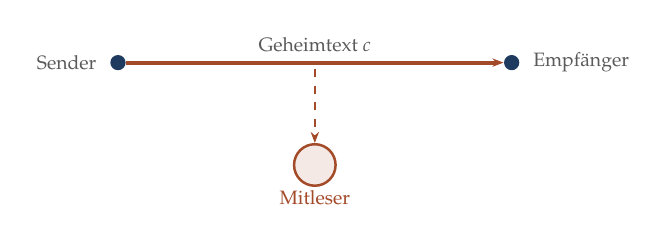
\begin{tikzpicture}[scale=1.0]
\node[knoten] (a) at (0,0) {};
\node[knoten] (b) at (5.0,0) {};
\node[knotenr] (e) at (2.5,-1.3) {};
\draw[kanted, -{Stealth[length=4pt]}] (a)--(b) node[midway,above,font=\scriptsize,color=grau] {Geheimtext $c$};
\draw[kante, akzent, dashed, -{Stealth[length=4pt]}] (2.5,-0.08)--(e);
\node[font=\scriptsize, color=grau, anchor=east] at (-0.15,0) {Sender};
\node[font=\scriptsize, color=grau, anchor=west] at (5.15,0) {Empfänger};
\node[font=\scriptsize, color=akzent, anchor=north] at (2.5,-1.5) {Mitleser};
\end{tikzpicture}
\end{center}

\schritt{Die Bestandteile}
\begin{center}
{\small
\renewcommand{\arraystretch}{1.5}
\begin{tabular}{@{}P{2.0cm}P{2.2cm}P{3.6cm}@{}}
\toprule
\textbf{Größe} & \textbf{Symbol} & \textbf{wer kennt sie}\\
\midrule
Klartext & $M$ & Sender, Empfänger\\
Schlüssel & $K$ & Sender, Empfänger\\
Geheimtext & $C$ & \textcolor{akzent}{alle}\\
\bottomrule
\end{tabular}}
\end{center}

\textbf{Die Frage:} Was heißt es, dass der Mitleser nichts erfährt --- und ist das erreichbar?

\begin{center}
\begin{minipage}{0.88\textwidth}
\kursiv{Die Antwort auf beide Teile gibt Shannons Arbeit von 1949, und sie benutzt genau die Größen aus Teil~II. \enquote{Nichts erfahren} heißt: Die Transinformation zwischen Klartext und Geheimtext ist null.}
\end{minipage}
\end{center}
\end{merksatz}

\begin{merksatz}
\boxtitel{Die Regel von Kerckhoffs}
\begin{center}
\begin{minipage}{0.9\textwidth}
\textbf{Das Verfahren gilt als bekannt. Geheim ist allein der Schlüssel.}
\end{minipage}
\end{center}

\begin{center}
\begin{minipage}{0.88\textwidth}
\kursiv{\Person{Auguste Kerckhoffs} formulierte diesen Grundsatz 1883. Er ist keine Vorsichtsmaßnahme, sondern eine Aussage über die Wirklichkeit: Verfahren werden bekannt --- durch Verrat, durch Nachbau, durch Veröffentlichung. \textbf{Ein Verfahren, dessen Sicherheit auf seiner Geheimhaltung beruht, ist genau einmal sicher.} Ein Schlüssel lässt sich dagegen austauschen.}
\end{minipage}
\end{center}
\end{merksatz}

\section{Warum klassische Verfahren brechen}

\begin{merksatz}
\boxtitel{Die einfache Ersetzung}
Jedem Buchstaben wird fest ein anderer zugeordnet. Der Schlüsselraum umfasst
\[ 26! \approx 4{,}03\cdot10^{26} \]
Möglichkeiten --- also
\[ \Ent(K) = \lb(26!) = 88{,}4 \ \text{Bit} . \]

\begin{center}
\begin{minipage}{0.9\textwidth}
\textbf{Das ist mehr als ein $80$-Bit-Schlüssel --- und das Verfahren ist mit Papier und Bleistift zu brechen.}
\end{minipage}
\end{center}

\schritt{Warum}
Die Ersetzung verändert die Buchstaben, nicht ihre Häufigkeiten. Im Geheimtext steht an der Stelle des \texttt{E} ein anderes Zeichen --- aber es ist genauso häufig.

\begin{center}
\begin{minipage}{0.88\textwidth}
\kursiv{Die Größe des Schlüsselraums ist also kein Maß für Sicherheit. \textbf{Entscheidend ist, ob der Geheimtext Struktur des Klartextes durchlässt} --- und genau das misst die Transinformation. Abschnitt 9.5 gibt an, wie viele Zeichen genügen, um den Schlüssel festzulegen.}
\end{minipage}
\end{center}
\end{merksatz}

\section{Perfekte Sicherheit}

\begin{definition}
\boxtitelm{Definition 9.1 --- Shannon, 1949}
Ein Verfahren heißt \Begriff{perfekt sicher}, wenn
\[ I(M;C) = 0 , \]
gleichbedeutend mit
\[ \Pr[M=m \mid C=c] = \Pr[M=m] \qquad\text{für alle } m,c . \]
\end{definition}

\begin{merksatz}
\boxtitel{Was das bedeutet}
\begin{center}
\begin{minipage}{0.9\textwidth}
\textbf{Der Geheimtext verändert die Einschätzung des Mitlesers über den Klartext nicht im Geringsten.} Er ist genau so klug wie vorher.
\end{minipage}
\end{center}

\begin{center}
\begin{minipage}{0.88\textwidth}
\kursiv{Das ist eine sehr starke Forderung --- und die einzige Sicherheitsdefinition dieses Bandes, die ohne jede Annahme über die Rechenkraft des Gegners auskommt. \textbf{Sie gilt auch gegen einen Gegner mit unbegrenzter Rechenzeit}, denn es gibt schlicht nichts zu berechnen.}
\end{minipage}
\end{center}

\schritt{Was sie nicht fordert}
Der Mitleser darf durchaus etwas über den Klartext wissen --- etwa dass es ein Befund ist. Er darf nur durch den Geheimtext nichts \kursiv{hinzulernen}.
\end{merksatz}

\begin{merksatz}
\boxtitel{Satz 9.2 --- der Einmalschlüssel ist perfekt sicher}
Sei $M$ eine Bitfolge der Länge $n$ und $K$ eine gleichverteilte, unabhängige Bitfolge derselben Länge. Dann ist
\[ C = M \oplus K \]
perfekt sicher.

\schritt{Beweis}
Für festes $m$ und beliebiges $c$:
\[ \Pr[C=c\mid M=m] = \Pr[K = c\oplus m] = 2^{-n} \]
--- denn $K$ ist gleichverteilt, und zu jedem Paar $(c,m)$ gehört genau ein Schlüssel.

Diese Wahrscheinlichkeit hängt \kursiv{nicht} von $m$ ab. Also sind $C$ und $M$ unabhängig, und nach Satz 4.5 ist $I(M;C) = 0$. $\blacksquare$

\schritt{Ein Zahlenbeispiel}
\begin{center}
{\small
\renewcommand{\arraystretch}{1.5}
\begin{tabular}{@{}P{2.6cm}P{2.8cm}@{}}
\toprule
Klartext $M$ & \texttt{01001000}\\
Schlüssel $K$ & \texttt{11010110}\\
\midrule
Geheimtext $C$ & \texttt{10011110}\\
\bottomrule
\end{tabular}}
\end{center}

\kursiv{Entschlüsseln:} $C \oplus K = \texttt{01001000} = M$ \checkmark

\schritt{Warum der Mitleser nichts erfährt}
Zu \kursiv{jedem} denkbaren Klartext gibt es einen Schlüssel, der genau diesen Geheimtext erzeugt hätte:

\begin{center}
\renewcommand{\arraystretch}{1.48}
\begin{tabular}{@{}P{2.4cm}P{2.4cm}P{2.4cm}@{}}
\toprule
\textbf{Klartext} & \textbf{nötiger Schlüssel} & \\
\midrule
\texttt{01001000} & \texttt{11010110} & \\
\texttt{01000001} & \texttt{11011111} & \\
\texttt{11111111} & \texttt{01100001} & \\
\bottomrule
\end{tabular}
\end{center}

\begin{center}
\begin{minipage}{0.9\textwidth}
\textbf{Alle drei sind gleich wahrscheinlich.} Der Geheimtext schließt keinen Klartext aus.
\end{minipage}
\end{center}
\end{merksatz}

\section{Shannons Schranke}

\begin{merksatz}
\boxtitel{Satz 9.3 --- der Schlüssel muss so groß sein wie die Nachricht}
Ist ein Verfahren perfekt sicher, so gilt
\[ \Ent(K) \ \ge\ \Ent(M) . \]

\schritt{Beweis --- Schritt 1: die Voraussetzung}
Perfekte Sicherheit bedeutet $I(M;C)=0$, also nach Definition 4.1
\[ \Ent(M\mid C) = \Ent(M) . \]

\schritt{Schritt 2 --- der Empfänger kann entschlüsseln}
Aus $C$ und $K$ ergibt sich $M$ eindeutig:
\[ \Ent(M\mid C,K) = 0 . \]

\schritt{Schritt 3 --- die Abschätzung}
\begin{align*}
\Ent(M\mid C) &\le \Ent(M,K\mid C) && \text{(mehr Größen, mehr Ungewissheit)}\\
&= \Ent(K\mid C) + \Ent(M\mid K,C) && \text{(Kettenregel)}\\
&= \Ent(K\mid C) + 0 && \text{(Schritt 2)}\\
&\le \Ent(K) && \text{(Satz 2.6)}
\end{align*}

\schritt{Schritt 4 --- zusammensetzen}
\[ \Ent(M) = \Ent(M\mid C) \ \le\ \Ent(K) \]
$\blacksquare$

\begin{center}
\begin{minipage}{0.9\textwidth}
\textbf{Perfekte Sicherheit verlangt einen Schlüssel, der mindestens so viel Ungewissheit trägt wie die Nachricht.}
\end{minipage}
\end{center}

\begin{center}
\begin{minipage}{0.88\textwidth}
\kursiv{Der Beweis benutzt nur die Kettenregel und Satz 2.6 --- also Werkzeuge aus Kapitel~2. \textbf{Die mathematische Kryptographie beginnt mit einem Satz, dessen Beweis vier Zeilen Informationstheorie ist.} Und der Satz ist ein Unmöglichkeitsergebnis: Er sagt nicht, wie man sicher verschlüsselt, sondern was es kostet.}
\end{minipage}
\end{center}
\end{merksatz}

\begin{warnung}
\boxtitelr{Warum der Einmalschlüssel kaum benutzt wird}
\begin{center}
{\small
\renewcommand{\arraystretch}{1.52}
\begin{tabular}{@{}P{2.4cm}P{6.2cm}@{}}
\toprule
\textbf{Schlüssellänge} & Wer ein Gigabyte übertragen will, muss vorher ein Gigabyte Schlüssel sicher austauschen.\\
\textbf{Das Henne-Ei-Problem} & Wenn man einen sicheren Kanal für den Schlüssel hat, könnte man darüber gleich die Nachricht senden.\\
\textbf{Einmalig} & Der Name ist Programm. Wird ein Schlüssel zweimal verwendet, bricht alles zusammen.\\
\textbf{Echter Zufall} & Der Schlüssel muss gleichverteilt sein. Ein Pseudozufallsgenerator zerstört die Perfektheit.\\
\bottomrule
\end{tabular}}
\end{center}

\schritt{Zur dritten Zeile}
Werden $M_1$ und $M_2$ mit demselben $K$ verschlüsselt, so gilt
\[ C_1 \oplus C_2 = M_1 \oplus M_2 . \]

\begin{center}
\begin{minipage}{0.9\textwidth}
\textbf{Der Schlüssel fällt heraus.} Übrig bleibt die Summe zweier Klartexte --- und die ist mit Sprachstatistik zu trennen.
\end{minipage}
\end{center}

\begin{center}
\begin{minipage}{0.88\textwidth}
\kursiv{Genau das geschah tatsächlich: Das Venona-Projekt der amerikanischen Dienste konnte zwischen 1943 und 1980 sowjetische Funksprüche entziffern, weil während des Krieges Schlüsselblöcke doppelt gedruckt und verteilt worden waren. \textbf{Ein beweisbar unbrechbares Verfahren wurde durch einen Verfahrensfehler gebrochen} --- und das ist die Regel, nicht die Ausnahme.}
\end{minipage}
\end{center}
\end{warnung}

\section{Die Unizitätsdistanz}

\begin{merksatz}
\boxtitel{Wenn der Schlüssel zu kurz ist}
Ist $\Ent(K) < \Ent(M)$, so ist das Verfahren nicht perfekt sicher --- aber wie unsicher?

\schritt{Der Gedanke}
Jedes Zeichen des Klartextes trägt Redundanz. Natürliche Sprache hat eine Entropierate von etwa $1{,}5$ Bit je Zeichen bei einem Alphabet von $26$ Zeichen:
\[ D = \lb 26 - 1{,}5 = 4{,}70 - 1{,}5 = 3{,}2 \ \text{Bit je Zeichen} \]

\begin{center}
\begin{minipage}{0.9\textwidth}
\textbf{Jedes Zeichen Geheimtext liefert dem Angreifer etwa $D$ Bit an Auskunft über den Schlüssel.} Nach $\Ent(K)/D$ Zeichen ist der Schlüssel festgelegt.
\end{minipage}
\end{center}
\end{merksatz}

\begin{definition}
\boxtitelm{Definition 9.4 --- Unizitätsdistanz}
\[ U = \frac{\Ent(K)}{D} \]
--- die Länge des Geheimtextes, ab der im Mittel nur noch ein Schlüssel zu einem sinnvollen Klartext führt.
\end{definition}

\begin{merksatz}
\boxtitel{Die Werte}
\begin{center}
{\small
\renewcommand{\arraystretch}{1.48}
\begin{tabular}{@{}P{2.6cm}P{2.2cm}P{2.8cm}@{}}
\toprule
\textbf{Verfahren} & $\Ent(K)$ & $U$ in Zeichen\\
\midrule
Cäsar & $4{,}70$ & $1{,}5$\\
Vigenère, $t=5$ & $23{,}50$ & $7{,}3$\\
Substitution & $88{,}38$ & $\mathbf{27{,}6}$\\
$128$-Bit-Schlüssel & $128$ & $40$\\
$256$-Bit-Schlüssel & $256$ & $80$\\
Einmalschlüssel & $= \Ent(M)$ & \textcolor{gruen}{$\infty$}\\
\bottomrule
\end{tabular}}
\end{center}

\begin{center}
\begin{minipage}{0.9\textwidth}
\textbf{Bei der einfachen Ersetzung genügen rund achtundzwanzig Buchstaben, um den Schlüssel eindeutig festzulegen.}
\end{minipage}
\end{center}

\begin{center}
\begin{minipage}{0.88\textwidth}
\kursiv{Das erklärt die Erfahrung jedes Rätsellösers: Kurze Kryptogramme sind mehrdeutig, ab etwa dreißig Zeichen gibt es nur noch eine sinnvolle Lesart. \textbf{Die Zahl folgt aus der Redundanz der Sprache, nicht aus einem Verfahren.}}
\end{minipage}
\end{center}

\schritt{Der entscheidende Vorbehalt}
\begin{center}
\begin{minipage}{0.9\textwidth}
\textbf{Die Unizitätsdistanz sagt, ab wann der Schlüssel \kursiv{bestimmt} ist --- nicht, wie man ihn findet.}
\end{minipage}
\end{center}

\begin{center}
\begin{minipage}{0.88\textwidth}
\kursiv{Bei einem $128$-Bit-Schlüssel ist nach vierzig Zeichen eindeutig festgelegt, welcher es ist. Ihn zu finden erfordert das Durchprobieren von $2^{128}$ Möglichkeiten --- und genau darauf beruht die gesamte moderne Kryptographie. \textbf{Sie tauscht informationstheoretische Sicherheit gegen rechnerische} und lebt davon, dass die Umsetzung der einen in die andere unpraktikabel ist.}
\end{minipage}
\end{center}

\schritt{Und die Folgerung für die Praxis}
Komprimiert man den Klartext vor der Verschlüsselung, so sinkt $D$ --- im Idealfall auf null.

\begin{center}
\begin{minipage}{0.88\textwidth}
\kursiv{Bei einem perfekt komprimierten Klartext wäre $U = \infty$ auch bei kurzem Schlüssel: Es gäbe keinen Anhaltspunkt, welcher Entschlüsselungsversuch sinnvoll ist. \textbf{Kompression vor Verschlüsselung ist daher kein Luxus, sondern eine Sicherheitsmaßnahme} --- und der einzige Punkt, an dem sich Teil~I und Teil~IV unmittelbar berühren.}
\end{minipage}
\end{center}
\end{merksatz}

\section{Der Bruchfall}

\begin{warnung}
\boxtitelr{Was perfekte Sicherheit nicht leistet}
\begin{center}
{\small
\renewcommand{\arraystretch}{1.52}
\begin{tabular}{@{}P{2.4cm}P{6.2cm}@{}}
\toprule
\textbf{Keine Echtheit} & Der Empfänger weiß nicht, ob die Nachricht vom richtigen Absender stammt.\\
\textbf{Keine Unversehrtheit} & Der Geheimtext lässt sich gezielt verändern.\\
\textbf{Keine Verkehrsdaten} & Dass gesendet wurde, wann und wie lang, bleibt sichtbar.\\
\bottomrule
\end{tabular}}
\end{center}

\schritt{Zur zweiten Zeile --- die Formbarkeit}
Kippt ein Angreifer im Geheimtext das letzte Bit, so kippt es auch im Klartext:
\[ (C \oplus \delta)\oplus K = M \oplus \delta \]

\begin{center}
\begin{minipage}{0.9\textwidth}
\textbf{Ein Angreifer, der den Klartext nicht kennt, kann ihn dennoch gezielt verändern.}
\end{minipage}
\end{center}

\begin{center}
\begin{minipage}{0.88\textwidth}
\kursiv{Bei einer Dosierungsangabe wäre das folgenschwer: Aus \enquote{$5$ mg} lässt sich ohne Kenntnis des Klartextes ein anderer Wert machen, wenn man weiß, an welcher Stelle die Zahl steht. \textbf{Perfekte Geheimhaltung und Unversehrtheit sind völlig verschiedene Eigenschaften}, und Kapitel~11 behandelt die zweite.}
\end{minipage}
\end{center}

\schritt{Zur dritten Zeile}
\begin{center}
\begin{minipage}{0.88\textwidth}
\kursiv{Dass eine Praxis um drei Uhr nachts eine verschlüsselte Nachricht an die Onkologie sendet, sagt bereits etwas --- unabhängig vom Inhalt. Die Verkehrsdatenanalyse ist in der Praxis oft ergiebiger als der Angriff auf die Verschlüsselung, und sie wird von keiner Sicherheitsdefinition dieses Bandes erfasst.}
\end{minipage}
\end{center}
\end{warnung}

\section{Übungsaufgaben}

\begin{aufgabe}
\boxtitel{Aufgabe 9.1 --- Der Einmalschlüssel}
Gegeben sei der Geheimtext \texttt{11010011} eines $8$-Bit-Einmalschlüssels.
\begin{center}
{\small
\renewcommand{\arraystretch}{1.4}
\begin{tabular}{@{}P{0.8cm}P{7.6cm}@{}}
\toprule
(a) & Welcher Schlüssel liefert den Klartext \texttt{01000001}?\\
(b) & Welcher liefert \texttt{01011010}?\\
(c) & Was folgt daraus für den Mitleser?\\
(d) & Der Angreifer kippt Bit $3$ und $8$. Was empfängt der Empfänger?\\
\bottomrule
\end{tabular}}
\end{center}

\loesung
\schritt{(a)}
\[ K = C \oplus M = \texttt{11010011} \oplus \texttt{01000001} = \texttt{10010010} \]

\kursiv{Probe:} $\texttt{10010010}\oplus\texttt{01000001} = \texttt{11010011}$ \checkmark

\schritt{(b)}
\[ K = \texttt{11010011} \oplus \texttt{01011010} = \texttt{10001001} \]

\schritt{(c)}
Beide Schlüssel sind gleich wahrscheinlich --- jeder der $256$ möglichen Schlüssel liefert genau einen der $256$ möglichen Klartexte.

\begin{center}
\begin{minipage}{0.9\textwidth}
\textbf{Der Mitleser kann keinen Klartext ausschließen und keinen bevorzugen.} Das ist Satz 9.2 in einem Einzelfall.
\end{minipage}
\end{center}

\schritt{(d) Die Formbarkeit}
Die Maske lautet $\delta = \texttt{00100001}$ (Bit $3$ und $8$, von links gezählt).
\[ C' = \texttt{11010011}\oplus\texttt{00100001} = \texttt{11110010} \]

Der Empfänger entschlüsselt mit dem richtigen $K$:
\[ M' = C'\oplus K = (C\oplus\delta)\oplus K = M \oplus \delta \]

\kursiv{Bei $M = \texttt{01000001}$:}
\[ M' = \texttt{01000001}\oplus\texttt{00100001} = \texttt{01100000} \]

\begin{center}
\begin{minipage}{0.9\textwidth}
\textbf{Der Empfänger erhält eine veränderte Nachricht und bemerkt nichts.}
\end{minipage}
\end{center}

\schritt{Schritt 5 --- Die Deutung}
\begin{center}
\begin{minipage}{0.88\textwidth}
\kursiv{Der Angreifer musste $M$ nicht kennen, um $M$ gezielt zu verändern. Er hat vollständige Kontrolle über die Differenz. \textbf{Wer eine Zahl an bekannter Stelle vermutet, kann sie gezielt verfälschen} --- und beim Einmalschlüssel ist diese Verfälschung nicht erkennbar. Die Abhilfe ist ein Beglaubigungscode, Kapitel~11.}
\end{minipage}
\end{center}
\end{aufgabe}

\begin{aufgabe}
\boxtitel{Aufgabe 9.2 --- Shannons Schranke anwenden}
Ein Klinikum will täglich $500$ Befunde von je $2$ Kilobyte perfekt sicher übertragen. Wie viel Schlüsselmaterial ist nötig, und was bedeutet das?

\loesung
\schritt{Schritt 1 --- Das Nachrichtenvolumen}
\[ 500 \cdot 2\,\text{kB} = 1000\,\text{kB} \approx 10^{6} \ \text{Byte} = 8\cdot10^{6} \ \text{Bit} \]

\schritt{Schritt 2 --- Die Schranke}
Nach Satz 9.3 muss $\Ent(K) \ge \Ent(M)$ gelten. Bei unkomprimierten Befunden ist $\Ent(M)$ deutlich kleiner als die Bitzahl --- Text ist redundant.

\kursiv{Mit einer Entropierate von $1{,}5$ Bit je Zeichen und $10^{6}$ Zeichen:}
\[ \Ent(M) \approx 1{,}5\cdot10^{6} \ \text{Bit} \]

\schritt{Schritt 3 --- Die praktische Folgerung}
\begin{center}
\renewcommand{\arraystretch}{1.48}
\begin{tabular}{@{}P{2.8cm}P{2.4cm}P{2.4cm}@{}}
\toprule
& \textbf{je Tag} & \textbf{je Jahr}\\
\midrule
Unkomprimiert & $1$ MB & $365$ MB\\
Komprimiert & $188$ kB & $69$ MB\\
\bottomrule
\end{tabular}
\end{center}

\begin{center}
\begin{minipage}{0.9\textwidth}
\textbf{Selbst nach Kompression müssten jährlich rund $69$ Megabyte Schlüsselmaterial sicher ausgetauscht werden.}
\end{minipage}
\end{center}

\schritt{Schritt 4 --- Warum das den Ansatz erledigt}
Der Schlüssel muss über einen sicheren Kanal übertragen werden --- persönlich, per Kurier, auf einem versiegelten Datenträger.

\begin{center}
\begin{minipage}{0.88\textwidth}
\kursiv{Hätte man einen solchen Kanal für $69$ Megabyte, so könnte man darüber gleich die Befunde senden. \textbf{Der Einmalschlüssel verschiebt das Problem, statt es zu lösen} --- er verwandelt \enquote{sicher übertragen} in \enquote{vorher sicher übertragen}.}
\end{minipage}
\end{center}

\schritt{Schritt 5 --- Wo er dennoch eingesetzt wird}
\begin{center}
{\small
\renewcommand{\arraystretch}{1.5}
\begin{tabular}{@{}P{2.4cm}P{6.2cm}@{}}
\toprule
\textbf{Kleine Mengen} & Diplomatische Kurzmitteilungen, bei denen wenige hundert Bit genügen.\\
\textbf{Vorratshaltung} & Der Schlüssel wird zu einem Zeitpunkt ausgetauscht, zu dem ein sicherer Kanal vorhanden ist, und später verbraucht.\\
\textbf{Langfristigkeit} & Nachrichten, die auch in fünfzig Jahren geheim bleiben müssen --- wo keine rechnerische Annahme trägt.\\
\bottomrule
\end{tabular}}
\end{center}

\begin{center}
\begin{minipage}{0.88\textwidth}
\kursiv{Die dritte Zeile ist heute wieder aktuell: Wer davon ausgeht, dass ein Quantenrechner die Verfahren aus Teil~V bricht, muss annehmen, dass heute aufgezeichneter Verkehr später entschlüsselt wird. \textbf{Gegen diese Sorge hilft nur informationstheoretische Sicherheit} --- Kapitel~15 kommt darauf zurück.}
\end{minipage}
\end{center}
\end{aufgabe}

\begin{aufgabe}
\boxtitel{Aufgabe 9.3 --- Unizitätsdistanz}
Bestimmen Sie die Unizitätsdistanz für ein Vigenère-Verfahren mit der Schlüssellänge $t$ und geben Sie an, ab welchem $t$ ein Text von $200$ Zeichen mehrdeutig bleibt.

\loesung
\schritt{Schritt 1 --- Die Schlüsselentropie}
Der Schlüssel besteht aus $t$ gleichverteilten Buchstaben:
\[ \Ent(K) = t\cdot\lb 26 = 4{,}70\,t \ \text{Bit} \]

\schritt{Schritt 2 --- Die Unizitätsdistanz}
\[ U = \frac{4{,}70\,t}{3{,}2} = 1{,}47\,t \]

\begin{center}
{\small
\renewcommand{\arraystretch}{1.48}
\begin{tabular}{@{}P{1.6cm}P{2.2cm}P{2.4cm}@{}}
\toprule
$t$ & $\Ent(K)$ & $U$\\
\midrule
$1$ & $4{,}70$ & $1{,}5$\\
$5$ & $23{,}50$ & $7{,}3$\\
$20$ & $94{,}00$ & $29{,}4$\\
$100$ & $470{,}0$ & $146{,}9$\\
$136$ & $639{,}2$ & $\mathbf{199{,}8}$\\
\bottomrule
\end{tabular}}
\end{center}

\schritt{Schritt 3 --- Die Antwort}
\[ 1{,}47\,t \ >\ 200 \quad\Longrightarrow\quad t \ >\ 136 \]

\begin{center}
\begin{minipage}{0.9\textwidth}
\textbf{Erst ab einer Schlüssellänge von $137$ Zeichen bleibt ein Text von $200$ Zeichen mehrdeutig.}
\end{minipage}
\end{center}

\schritt{Schritt 4 --- Die Deutung}
Der Schlüssel muss also mehr als zwei Drittel der Textlänge haben.

\begin{center}
\begin{minipage}{0.88\textwidth}
\kursiv{Das ist Satz 9.3 in abgeschwächter Form: Perfekte Sicherheit verlangt $\Ent(K)\ge\Ent(M)$, also $4{,}70\,t \ge 1{,}5\cdot200 = 300$, mithin $t \ge 64$. Die Unizitätsdistanz verlangt mehr, weil sie nicht Perfektheit fordert, sondern nur Mehrdeutigkeit \kursiv{bei der Suche} --- und dafür muss die Redundanz über die \kursiv{gesamte} Alphabetgröße gemessen werden.}
\end{minipage}
\end{center}

\schritt{Schritt 5 --- Warum Vigenère trotzdem fiel}
Bei $t = 20$ und einem Text von $2000$ Zeichen liegt $U = 29$ weit unter der Textlänge --- der Schlüssel ist eindeutig bestimmt.

\begin{center}
\begin{minipage}{0.88\textwidth}
\kursiv{Und er ist auch \kursiv{findbar}: Kennt man $t$, so zerfällt der Text in $t$ Teiltexte, von denen jeder nur mit einem Cäsar-Verfahren verschlüsselt ist --- und dafür genügt die Häufigkeitsanalyse. Die Periode $t$ wiederum verrät sich durch Wiederholungen im Geheimtext. \textbf{Die Unizitätsdistanz sagt, dass es geht; das Kasiski-Verfahren sagt, wie.}}
\end{minipage}
\end{center}

\schritt{Schritt 6 --- Der Grenzfall}
Bei $t \ge$ Textlänge und einem zufälligen Schlüssel wird Vigenère zum Einmalschlüssel.

\begin{center}
\begin{minipage}{0.86\textwidth}
\kursiv{Genau so wurde er historisch verwendet --- als \enquote{laufender Schlüssel} mit einem Buchtext als Quelle. Das ist nicht perfekt sicher, weil der Buchtext selbst redundant ist: Man sucht Schlüssel, die zugleich sinnvollen Klartext und sinnvollen Schlüsseltext liefern.}
\end{minipage}
\end{center}
\end{aufgabe}

\begin{geschichte}
\boxtitelg{Ein Patent und ein Beweis}
\Person{Gilbert Vernam} (1890--1960) meldete 1919 für die amerikanische Telefongesellschaft ein Verfahren an, das Fernschreibzeichen mit einem Lochstreifen verknüpfte.

\begin{center}
\begin{minipage}{0.9\textwidth}
\kursiv{Vernams ursprüngliches Verfahren benutzte einen sich wiederholenden Streifen --- also einen Vigenère mit langer Periode. \Person{Joseph Mauborgne} vom amerikanischen Fernmeldewesen erkannte, dass die Wiederholung die Schwäche ist, und schlug einen Streifen zufälliger Zeichen vor, der nur einmal benutzt wird. \textbf{Die entscheidende Idee war nicht die Verknüpfung, sondern die Einmaligkeit.}}
\end{minipage}
\end{center}

\schritt{Der Beweis}
\Person{Claude Shannon} bewies 1949 in \kursiv{Communication Theory of Secrecy Systems}, dass das Verfahren perfekt sicher ist --- und dass kein Verfahren mit kürzerem Schlüssel es sein kann.

\begin{center}
\begin{minipage}{0.9\textwidth}
\kursiv{Die Arbeit entstand bereits 1945 als vertraulicher Bericht und wurde erst nach der Freigabe veröffentlicht. Sie enthält neben Satz 9.3 die Unizitätsdistanz und die Begriffe \kursiv{Verwirrung} und \kursiv{Verwischung}, die den Entwurf von Blockchiffren bis heute leiten --- Kapitel~10.}
\end{minipage}
\end{center}

\schritt{Vorläufer}
\Person{Frank Miller}, ein amerikanischer Bankier, beschrieb 1882 in einem Codebuch für Telegramme ein Verfahren mit Einmalschlüsseln --- siebenunddreißig Jahre vor Vernam.

\begin{center}
\begin{minipage}{0.9\textwidth}
\kursiv{Die Arbeit wurde erst 2011 wiederentdeckt und ausgewertet. Sie enthält bereits die Forderung nach Zufälligkeit und Einmaligkeit. Ob Vernam davon wusste, ist unbekannt.}
\end{minipage}
\end{center}

\schritt{Venona}
Zwischen 1943 und 1980 entzifferten amerikanische Dienste rund dreitausend sowjetische Funksprüche.

\begin{center}
\begin{minipage}{0.9\textwidth}
\kursiv{Die Ursache war ein Herstellungsfehler: Unter dem Druck des Krieges wurden Schlüsselblöcke doppelt gedruckt und an verschiedene Stellen verteilt. \textbf{Von Millionen Funksprüchen waren nur wenige Prozent betroffen --- und das genügte.} Das Projekt enttarnte unter anderem die Spionage im Manhattan-Projekt. Es ist der lehrreichste Fall der Kryptographiegeschichte: Nicht die Mathematik versagte, sondern die Papierverwaltung.}
\end{minipage}
\end{center}
\end{geschichte}

\begin{forschung}
\boxtitelp{Informationstheoretische Sicherheit heute}
\begin{center}
{\small
\renewcommand{\arraystretch}{1.45}
\begin{tabular}{@{}P{3.2cm}P{5.0cm}@{}}
\toprule
\textbf{Quanten\-schlüsseltausch} & Zwei Parteien erzeugen gemeinsames Schlüsselmaterial; Abhören ist physikalisch nachweisbar.\\
\textbf{Geheimnis\-teilung} & Ein Geheimnis wird so auf $n$ Teile verteilt, dass je $k$ genügen und $k-1$ nichts verraten.\\
\textbf{Abhörkanäle} & Ist der Kanal zum Angreifer schlechter als der zum Empfänger, lässt sich ohne Schlüssel geheim übertragen.\\
\bottomrule
\end{tabular}}
\end{center}

\schritt{Zur zweiten Zeile}
\Person{Adi Shamir} gab 1979 ein Verfahren an, das auf der Polynominterpolation aus Kapitel~6 beruht.

\begin{center}
\begin{minipage}{0.88\textwidth}
\kursiv{Man wählt ein Polynom vom Grad $k-1$, dessen konstantes Glied das Geheimnis ist, und verteilt $n$ Auswertungen. Je $k$ Punkte bestimmen das Polynom; $k-1$ Punkte lassen jeden Wert an der Stelle null gleich möglich. \textbf{Das ist beweisbare Sicherheit im Sinn von Definition 9.1} --- und dasselbe mathematische Prinzip wie beim Reed-Solomon-Code, nur in umgekehrter Absicht.}
\end{minipage}
\end{center}

\schritt{Zur dritten Zeile}
\Person{Aaron Wyner} zeigte 1975: Ist der Kanal zum Abhörer schlechter, so gibt es eine positive \Begriff{Geheimhaltungskapazität}.

\begin{center}
\begin{minipage}{0.88\textwidth}
\kursiv{Sie beträgt beim gedächtnislosen Kanal gerade die Differenz der Kapazitäten. Das ist bemerkenswert: \textbf{Man kann ohne vorher ausgetauschten Schlüssel geheim übertragen}, sofern der Gegner physikalisch benachteiligt ist. Praktisch ist die Voraussetzung schwer zu sichern --- man müsste wissen, wie gut der Empfang des Abhörers ist.}
\end{minipage}
\end{center}
\end{forschung}

\begin{merksatz}
\boxtitel{Was Sie jetzt können}
\begin{center}
\renewcommand{\arraystretch}{1.5}
\begin{tabular}{@{}P{3.0cm}P{5.6cm}@{}}
\toprule
\textbf{Kerckhoffs} & nur der Schlüssel ist geheim\\
\textbf{Definition 9.1} & $I(M;C) = 0$\\
\textbf{Satz 9.2} & Einmalschlüssel ist perfekt\\
\textbf{Satz 9.3} & $\Ent(K)\ge\Ent(M)$ --- vier Zeilen\\
\textbf{Definition 9.4} & Unizitätsdistanz $\Ent(K)/D$\\
\bottomrule
\end{tabular}
\end{center}

\begin{center}
\begin{minipage}{0.88\textwidth}
\kursiv{Satz 9.3 macht perfekte Sicherheit praktisch unbrauchbar. Das nächste Kapitel gibt sie auf --- und ersetzt sie durch eine Annahme, die niemand beweisen kann.}
\end{minipage}
\end{center}
\end{merksatz}

\chapter{Blockchiffren}

\section{Der Übergang}

\begin{merksatz}
\boxtitel{Was Satz 9.3 erzwingt}
Perfekte Sicherheit verlangt einen Schlüssel, der so lang ist wie die Nachricht. Das ist praktisch unbrauchbar.

\begin{center}
\begin{minipage}{0.9\textwidth}
\textbf{Also gibt man sie auf --- und ersetzt sie durch eine schwächere Forderung.}
\end{minipage}
\end{center}

\begin{center}
{\small
\renewcommand{\arraystretch}{1.55}
\begin{tabular}{@{}P{2.6cm}P{6.0cm}@{}}
\toprule
\textbf{Informations\-theoretisch} & Der Geheimtext enthält \kursiv{keine} Information über den Klartext. Gilt gegen jeden Gegner.\\
\textbf{Rechnerisch} & Der Geheimtext enthält Information, aber kein Verfahren mit vertretbarem Aufwand kann sie gewinnen.\\
\bottomrule
\end{tabular}}
\end{center}

\begin{center}
\begin{minipage}{0.88\textwidth}
\kursiv{Der Unterschied ist grundsätzlich. Bei rechnerischer Sicherheit \kursiv{gibt} es die Information --- ein Gegner mit unbegrenzter Rechenzeit findet den Schlüssel stets, einfach durch Durchprobieren. \textbf{Die Sicherheit beruht allein darauf, dass niemand diese Rechenzeit hat.}}
\end{minipage}
\end{center}

\schritt{Die Zahlen}
\begin{center}
{\small
\renewcommand{\arraystretch}{1.48}
\begin{tabular}{@{}P{1.8cm}P{2.2cm}P{3.2cm}@{}}
\toprule
\textbf{Schlüssel} & \textbf{Möglich\-keiten} & \textbf{bei $10^{18}$ je Sekunde}\\
\midrule
$56$ Bit & $7{,}2\cdot10^{16}$ & $0{,}07$ Sekunden\\
$112$ Bit & $5{,}2\cdot10^{33}$ & $1{,}7\cdot10^{8}$ Jahre\\
$128$ Bit & $3{,}4\cdot10^{38}$ & $1{,}1\cdot10^{13}$ Jahre\\
$256$ Bit & $1{,}2\cdot10^{77}$ & $3{,}7\cdot10^{51}$ Jahre\\
\bottomrule
\end{tabular}}
\end{center}

\begin{center}
\begin{minipage}{0.88\textwidth}
\kursiv{Das Weltalter beträgt $1{,}4\cdot10^{10}$ Jahre. Bei $128$ Bit liegt die Suchdauer tausendmal darüber --- und die unterstellte Rate von einer Trillion Schlüsseln je Sekunde ist bereits großzügig. \textbf{Zwischen $56$ und $128$ Bit liegen keine zweieinhalb Größenordnungen, sondern zwanzig.}}
\end{minipage}
\end{center}
\end{merksatz}

\section{Verwirrung und Verwischung}

\begin{merksatz}
\boxtitel{Shannons zwei Entwurfsgrundsätze}
\begin{center}
{\small
\renewcommand{\arraystretch}{1.55}
\begin{tabular}{@{}P{2.4cm}P{6.2cm}@{}}
\toprule
\textbf{Verwirrung} & Der Zusammenhang zwischen Schlüssel und Geheimtext soll so verwickelt sein, dass er sich nicht durch einfache Gleichungen beschreiben lässt.\\
\textbf{Verwischung} & Jedes Bit des Klartextes soll jedes Bit des Geheimtextes beeinflussen --- die Struktur des Klartextes wird über den ganzen Block verteilt.\\
\bottomrule
\end{tabular}}
\end{center}

\begin{center}
\begin{minipage}{0.88\textwidth}
\kursiv{Beide stammen aus Shannons Arbeit von 1949 und sind bis heute die Leitlinien jedes Chiffrenentwurfs. \textbf{Die Verwischung ist die Antwort auf die Häufigkeitsanalyse aus Kapitel~9}: Wenn ein einzelnes Klartextzeichen den ganzen Block verändert, gibt es keine Zeichenhäufigkeiten mehr, die man zählen könnte.}
\end{minipage}
\end{center}
\end{merksatz}

\begin{merksatz}
\boxtitel{Das Lawinenkriterium}
\begin{center}
\begin{minipage}{0.9\textwidth}
\textbf{Ändert man ein Bit der Eingabe, so soll sich im Mittel die Hälfte der Ausgabebits ändern.}
\end{minipage}
\end{center}

\schritt{Warum genau die Hälfte}
Das ist das Verhalten einer zufälligen Abbildung. Jedes Ausgabebit kippt unabhängig mit Wahrscheinlichkeit $\frac12$.

\begin{center}
{\small
\renewcommand{\arraystretch}{1.48}
\begin{tabular}{@{}P{3.4cm}P{1.8cm}P{2.4cm}@{}}
\toprule
& \textbf{Wert} & \\
\midrule
Blocklänge & $128$ & \\
Erwartete Änderung & $64$ & \\
Standard\-abweichung & $5{,}66$ & $\sqrt{128/4}$\\
$\Pr[54\ldots74]$ & $0{,}937$ & \\
\bottomrule
\end{tabular}}
\end{center}

\begin{center}
\begin{minipage}{0.88\textwidth}
\kursiv{Ändern sich deutlich weniger oder deutlich mehr als $64$ Bit, so verhält sich die Chiffre nicht wie eine zufällige Abbildung --- und das ist angreifbar. \textbf{Das Prüfkriterium lautet nicht \enquote{möglichst viel Änderung}, sondern \enquote{genau so viel wie bei Zufall}.} Eine Chiffre, die \kursiv{alle} Bits kippt, wäre ebenso auffällig wie eine, die keines kippt.}
\end{minipage}
\end{center}
\end{merksatz}

\begin{merksatz}
\boxtitel{Der Aufbau in Runden}
Verwirrung und Verwischung erreicht man durch Wiederholung einfacher Bausteine.

\begin{center}
{\small
\renewcommand{\arraystretch}{1.5}
\begin{tabular}{@{}P{2.8cm}P{2.4cm}P{2.6cm}@{}}
\toprule
\textbf{Baustein} & \textbf{Wirkung} & \textbf{Umfang}\\
\midrule
Ersetzung & Verwirrung & wenige Bits\\
Vertauschung & Verwischung & ganzer Block\\
Schlüssel\-addition & bindet den Schlüssel & ganzer Block\\
\bottomrule
\end{tabular}}
\end{center}

\begin{center}
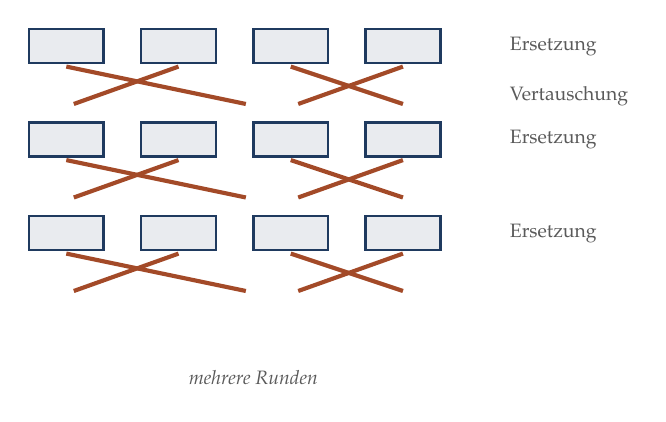
\begin{tikzpicture}[scale=0.95]
\foreach \r in {0,1,2} {
  \begin{scope}[yshift=-\r*1.25cm]
  \foreach \x in {0,1,2,3}
    \draw[tief, line width=0.9pt, fill=tief!10] (\x*1.5,0) rectangle ++(1.0,0.45);
  \node[font=\scriptsize, color=grau, anchor=west] at (6.3,0.22) {Ersetzung};
  \draw[kanted] (0.5,-0.05) -- (2.9,-0.55);
  \draw[kanted] (2.0,-0.05) -- (0.6,-0.55);
  \draw[kanted] (3.5,-0.05) -- (5.0,-0.55);
  \draw[kanted] (5.0,-0.05) -- (3.6,-0.55);
  \end{scope}
}
\node[font=\scriptsize, color=grau, anchor=west] at (6.3,-0.45) {Vertauschung};
\node[font=\scriptsize\itshape, color=grau] at (3.0,-4.2) {mehrere Runden};
\end{tikzpicture}
\end{center}

\begin{center}
\begin{minipage}{0.88\textwidth}
\kursiv{Nach wenigen Runden ist jedes Ausgabebit von jedem Eingabebit abhängig --- das nennt man \Begriff{vollständige Verwischung}. Die tatsächliche Rundenzahl liegt deutlich darüber: Der Advanced Encryption Standard erreicht vollständige Verwischung nach zwei Runden und benutzt zehn bis vierzehn. \textbf{Die überzähligen Runden sind der Sicherheitsabstand}, und der ist es, der ein Verfahren jahrzehntelang trägt.}
\end{minipage}
\end{center}
\end{merksatz}

\section{Betriebsarten}

\begin{merksatz}
\boxtitel{Eine Blockchiffre allein genügt nicht}
Sie verschlüsselt einen Block fester Länge --- etwa $128$ Bit. Nachrichten sind länger.

\begin{center}
{\small
\renewcommand{\arraystretch}{1.55}
\begin{tabular}{@{}P{1.8cm}P{3.0cm}P{3.6cm}@{}}
\toprule
\textbf{Art} & \textbf{Vorschrift} & \textbf{Eigenschaft}\\
\midrule
ECB & $C_i = E_K(M_i)$ & \textcolor{akzent}{unbrauchbar}\\
CBC & $C_i = E_K(M_i\oplus C_{i-1})$ & braucht Startwert\\
CTR & $C_i = M_i\oplus E_K(N\Vert i)$ & Stromchiffre\\
\bottomrule
\end{tabular}}
\end{center}
\end{merksatz}

\begin{warnung}
\boxtitelr{Warum ECB unbrauchbar ist}
\begin{center}
\begin{minipage}{0.9\textwidth}
\textbf{Gleiche Klartextblöcke ergeben gleiche Geheimtextblöcke.}
\end{minipage}
\end{center}

\schritt{Die Folge}
Der Geheimtext verrät, welche Blöcke übereinstimmen --- also die gesamte Wiederholungsstruktur der Nachricht.

\begin{center}
\begin{minipage}{0.88\textwidth}
\kursiv{Bei einem Bild bleiben die Umrisse sichtbar: Flächen gleicher Farbe werden zu Flächen gleicher Geheimtextblöcke. Das bekannteste Anschauungsbeispiel --- ein verschlüsseltes Pinguinbild, dessen Umriss erkennbar bleibt --- ist seit Jahren in jedem Lehrbuch.}
\end{minipage}
\end{center}

\schritt{In der Sprache von Kapitel 4}
\begin{center}
\begin{minipage}{0.9\textwidth}
\textbf{$I(M;C) > 0$, und zwar erheblich.} ECB verletzt die Grundforderung, ohne dass man irgendetwas brechen müsste.
\end{minipage}
\end{center}

\schritt{Bei Befunddaten}
\begin{center}
\begin{minipage}{0.88\textwidth}
\kursiv{Eine Datenbank mit einem Eintrag je Patient, blockweise verschlüsselt: Alle Patienten mit derselben Diagnose haben denselben Geheimtextblock. Man kennt die Diagnose nicht --- aber man kann die Patienten gruppieren und die Gruppengrößen mit der bekannten Häufigkeitsverteilung aus Kapitel~1 abgleichen. \textbf{Damit ist die häufigste Gruppe zugeordnet, und die zweithäufigste auch.} Es ist die Häufigkeitsanalyse aus Kapitel~9, auf Blöcke übertragen.}
\end{minipage}
\end{center}
\end{warnung}

\begin{merksatz}
\boxtitel{Die Abhilfe: Zufall hinzufügen}
\begin{center}
{\small
\renewcommand{\arraystretch}{1.5}
\begin{tabular}{@{}P{2.4cm}P{6.2cm}@{}}
\toprule
\textbf{CBC} & Ein zufälliger Startwert wird dem ersten Block zugemischt; jeder weitere Block erhält den vorangegangenen Geheimtext.\\
\textbf{CTR} & Ein Zähler wird verschlüsselt und liefert einen Schlüsselstrom; die Blockchiffre wird nie auf den Klartext angewandt.\\
\bottomrule
\end{tabular}}
\end{center}

\begin{center}
\begin{minipage}{0.9\textwidth}
\textbf{In beiden Fällen liefern gleiche Klartextblöcke verschiedene Geheimtextblöcke.} Dieselbe Nachricht zweimal verschlüsselt ergibt zwei völlig verschiedene Geheimtexte.
\end{minipage}
\end{center}

\schritt{Der Vergleich}
\begin{center}
{\small
\renewcommand{\arraystretch}{1.48}
\begin{tabular}{@{}P{2.2cm}P{2.0cm}P{2.0cm}P{2.0cm}@{}}
\toprule
& \textbf{ECB} & \textbf{CBC} & \textbf{CTR}\\
\midrule
Parallel & \textcolor{gruen}{ja} & \textcolor{akzent}{nein} & \textcolor{gruen}{ja}\\
Wahlfreier Zugriff & \textcolor{gruen}{ja} & teilweise & \textcolor{gruen}{ja}\\
Auffüllen nötig & ja & ja & \textcolor{gruen}{nein}\\
Sicher & \textcolor{akzent}{nein} & \textcolor{gruen}{ja} & \textcolor{gruen}{ja}\\
\bottomrule
\end{tabular}}
\end{center}

\begin{center}
\begin{minipage}{0.88\textwidth}
\kursiv{CTR verwandelt die Blockchiffre in eine Stromchiffre --- und damit in etwas, das dem Einmalschlüssel aus Kapitel~9 formal gleicht. \textbf{Der Unterschied ist, dass der Schlüsselstrom nicht zufällig, sondern nur \kursiv{nicht unterscheidbar} von zufällig ist.} Damit erbt CTR alle Eigenschaften des Einmalschlüssels --- einschließlich der unangenehmen.}
\end{minipage}
\end{center}
\end{merksatz}

\section{Der Bruchfall}

\begin{warnung}
\boxtitelr{Der Zählerwert darf sich nie wiederholen}
Wird bei CTR derselbe Zählerwert zweimal mit demselben Schlüssel verwendet, so entsteht derselbe Schlüsselstrom:
\[ C_1 \oplus C_2 = M_1 \oplus M_2 \]

\begin{center}
\begin{minipage}{0.9\textwidth}
\textbf{Das ist exakt der Venona-Fehler aus Kapitel~9} --- nur dass er hier nicht durch doppelt gedrucktes Papier entsteht, sondern durch einen Programmfehler.
\end{minipage}
\end{center}

\begin{center}
\begin{minipage}{0.88\textwidth}
\kursiv{Häufige Ursachen: ein Zähler, der nach einem Neustart wieder bei null beginnt; ein zufällig gewählter Startwert, der zu kurz ist; ein auf mehrere Geräte kopierter Schlüssel ohne abgestimmte Zählerbereiche. \textbf{Die Mathematik ist einwandfrei; die Umsetzung ist die Schwachstelle} --- und das ist die durchgehende Erfahrung dieses Fachs.}
\end{minipage}
\end{center}
\end{warnung}

\begin{warnung}
\boxtitelr{Die Geburtstagsschranke}
Bei einer Blocklänge von $n$ Bit treten nach etwa $2^{n/2}$ Blöcken Wiederholungen auf --- rein aus Zufall.

\begin{center}
{\small
\renewcommand{\arraystretch}{1.48}
\begin{tabular}{@{}P{2.2cm}P{1.8cm}P{2.2cm}P{2.2cm}@{}}
\toprule
\textbf{Chiffre} & $n$ & \textbf{Blöcke} & \textbf{Datenmenge}\\
\midrule
3DES & $64$ & $2^{32}$ & $\mathbf{34}$ \textbf{GB}\\
AES & $128$ & $2^{64}$ & $295$ Exabyte\\
\bottomrule
\end{tabular}}
\end{center}

\begin{center}
\begin{minipage}{0.9\textwidth}
\textbf{Bei $64$ Bit Blocklänge genügen $34$ Gigabyte, um eine Kollision wahrscheinlich zu machen.}
\end{minipage}
\end{center}

\begin{center}
\begin{minipage}{0.88\textwidth}
\kursiv{Bei CBC verrät eine Kollision $C_i = C_j$ unmittelbar $M_i \oplus M_j$. Genau darauf beruht ein 2016 veröffentlichter Angriff auf Verbindungen, die noch 3DES verwendeten. \textbf{Das Verfahren war nicht gebrochen --- die Blocklänge war zu kurz.} Bei einer Dauerverbindung sind $34$ Gigabyte binnen Stunden erreicht.}
\end{minipage}
\end{center}

\schritt{Die Lehre}
\begin{center}
\begin{minipage}{0.9\textwidth}
\textbf{Schlüssellänge und Blocklänge sind verschiedene Größen.} $3$DES hat $112$ Bit Schlüssel und ist dennoch begrenzt --- durch die $64$ Bit Blocklänge.
\end{minipage}
\end{center}
\end{warnung}

\begin{warnung}
\boxtitelr{Und drei weitere Fallen}
\begin{center}
{\small
\renewcommand{\arraystretch}{1.5}
\begin{tabular}{@{}P{2.4cm}P{6.2cm}@{}}
\toprule
\textbf{Keine Echtheit} & Auch CBC und CTR sind formbar. Verschlüsselung allein schützt nicht vor gezielter Veränderung.\\
\textbf{Seitenkanäle} & Laufzeit, Stromverbrauch und Zwischenspeicherverhalten können den Schlüssel verraten, obwohl die Mathematik stimmt.\\
\textbf{Auffüllen} & Die Art, wie unvollständige Blöcke ergänzt werden, hat wiederholt zu Angriffen geführt.\\
\bottomrule
\end{tabular}}
\end{center}

\begin{center}
\begin{minipage}{0.88\textwidth}
\kursiv{Die zweite Zeile ist die unangenehmste, weil sie außerhalb des mathematischen Modells liegt. Ein Verfahren, dessen Rechenzeit vom Schlüssel abhängt, verrät ihn --- und die frühen Umsetzungen des Advanced Encryption Standard taten genau das, weil die Ersetzungstabelle im Zwischenspeicher schlüsselabhängig durchlaufen wurde. \textbf{Das Modell dieses Kapitels kennt nur Eingabe und Ausgabe; die Wirklichkeit hat mehr Kanäle.}}
\end{minipage}
\end{center}
\end{warnung}

\section{Übungsaufgaben}

\begin{aufgabe}
\boxtitel{Aufgabe 10.1 --- Der Lawineneffekt}
Eine Chiffre mit $64$ Bit Blocklänge wird geprüft: Bei Änderung eines Eingabebits ändern sich $18$ Ausgabebits. Ist das auffällig?

\loesung
\schritt{Schritt 1 --- Die Erwartung}
Bei einer zufälligen Abbildung kippt jedes Bit unabhängig mit $\frac12$:
\[ \mathbb{E} = 64\cdot0{,}5 = 32, \qquad \sigma = \sqrt{64\cdot0{,}25} = 4 \]

\schritt{Schritt 2 --- Der Abstand}
\[ \frac{18-32}{4} = -3{,}5 \ \text{Standardabweichungen} \]

\schritt{Schritt 3 --- Die Wahrscheinlichkeit}
Nach der Normalverteilungsnäherung (Band 12):
\[ \Pr[X \le 18] \approx \Pr[Z \le -3{,}5] = 2{,}3\cdot10^{-4} \]

\begin{center}
\begin{minipage}{0.9\textwidth}
\textbf{Ein solches Ergebnis tritt bei einer guten Chiffre etwa einmal unter viertausend Versuchen auf --- das ist auffällig.}
\end{minipage}
\end{center}

\schritt{Schritt 4 --- Die Einschränkung}
Prüft man alle $64$ Eingabebits, so hat man $64$ Versuche. Die Wahrscheinlichkeit, dass \kursiv{mindestens einer} so weit abweicht:
\[ 1-(1-2{,}3\cdot10^{-4})^{64} = 1{,}5\,\% \]

\begin{center}
\begin{minipage}{0.88\textwidth}
\kursiv{Das ist das Problem des mehrfachen Testens aus Band 17. \textbf{Ein einzelner auffälliger Wert unter vielen Prüfungen ist noch kein Befund} --- man müsste ihn an weiteren Eingaben bestätigen.}
\end{minipage}
\end{center}

\schritt{Schritt 5 --- Wann es ein Befund wäre}
Träte die Abweichung bei \kursiv{allen} Eingabebits auf, so wäre das systematisch:
\[ (2{,}3\cdot10^{-4})^{64} \approx 10^{-234} \]

\begin{center}
\begin{minipage}{0.88\textwidth}
\kursiv{Dann läge kein Zufall vor, sondern eine Struktur --- und Strukturen sind der Ansatzpunkt jedes Angriffs. \textbf{Die Prüfung des Lawinenkriteriums ist ein statistischer Test wie jeder andere}, mit denselben Fallstricken.}
\end{minipage}
\end{center}
\end{aufgabe}

\begin{aufgabe}
\boxtitel{Aufgabe 10.2 --- Betriebsarten}
Eine Befunddatenbank enthält $50\,000$ Einträge mit je einem Diagnosecode. Die Häufigkeiten sind die aus Kapitel~1. Welche Auskunft gibt ein ECB-verschlüsselter Auszug?

\loesung
\schritt{Schritt 1 --- Was sichtbar wird}
Jeder Diagnosecode ergibt stets denselben Geheimtextblock. Der Angreifer sieht acht verschiedene Blöcke mit ihren Häufigkeiten.

\schritt{Schritt 2 --- Die erwarteten Anzahlen}
\begin{center}
{\small
\renewcommand{\arraystretch}{1.48}
\begin{tabular}{@{}P{1.8cm}P{1.8cm}P{2.2cm}P{2.0cm}@{}}
\toprule
\textbf{Gruppe} & \textbf{Anteil} & \textbf{erwartet} & $\sigma$\\
\midrule
$A$, $B$ & $0{,}2500$ & $12\,500$ & $97$\\
$C$, $D$ & $0{,}1250$ & $6250$ & $74$\\
$E$--$H$ & $0{,}0625$ & $3125$ & $54$\\
\bottomrule
\end{tabular}}
\end{center}

\kursiv{Zur Standardabweichung:} $\sqrt{50\,000\cdot0{,}25\cdot0{,}75} = 96{,}8$.

\schritt{Schritt 3 --- Die Zuordnung}
Die drei Häufigkeitsstufen sind durch je etwa sechzig Standardabweichungen getrennt.

\begin{center}
\begin{minipage}{0.9\textwidth}
\textbf{Die Zuordnung der Stufen ist praktisch sicher.} Innerhalb einer Stufe --- etwa zwischen $A$ und $B$ --- gibt die Häufigkeit nichts her.
\end{minipage}
\end{center}

\schritt{Schritt 4 --- Was der Angreifer erfährt}
\begin{center}
{\small
\renewcommand{\arraystretch}{1.48}
\begin{tabular}{@{}P{2.6cm}P{2.4cm}P{2.6cm}@{}}
\toprule
\textbf{Auskunft} & \textbf{erhalten?} & \\
\midrule
Stufe je Eintrag & \textcolor{akzent}{ja} & drei Klassen\\
Genaue Gruppe & teilweise & bei $C$/$D$ zweideutig\\
Gleichheit zweier Einträge & \textcolor{akzent}{ja} & vollständig\\
\bottomrule
\end{tabular}}
\end{center}

\schritt{Schritt 5 --- Der Informationsgehalt}
Der Angreifer erfährt die Stufe. Die verbleibende Ungewissheit:
\begin{center}
\renewcommand{\arraystretch}{1.46}
\begin{tabular}{@{}P{2.2cm}P{2.2cm}P{2.6cm}@{}}
\toprule
\textbf{Stufe} & \textbf{Anteil} & \textbf{Restentropie}\\
\midrule
$\{A,B\}$ & $0{,}50$ & $1$ Bit\\
$\{C,D\}$ & $0{,}25$ & $1$ Bit\\
$\{E,\ldots,H\}$ & $0{,}25$ & $2$ Bit\\
\bottomrule
\end{tabular}
\end{center}

\[ \Ent(M\mid C) = 0{,}5\cdot1 + 0{,}25\cdot1 + 0{,}25\cdot2 = 1{,}25 \ \text{Bit} \]
\[ I(M;C) = \Ent(M) - \Ent(M\mid C) = 2{,}75 - 1{,}25 = \mathbf{1{,}50} \ \text{Bit} \]

\begin{center}
\begin{minipage}{0.9\textwidth}
\textbf{Mehr als die Hälfte der Information ist durchgesickert --- ohne dass die Chiffre gebrochen wurde.}
\end{minipage}
\end{center}

\schritt{Schritt 6 --- Die Abhilfe}
Bei CBC oder CTR mit wechselndem Startwert ist $I(M;C) = 0$ im Rahmen der rechnerischen Ununterscheidbarkeit.

\begin{center}
\begin{minipage}{0.88\textwidth}
\kursiv{Für eine \kursiv{durchsuchbare} Datenbank ist das allerdings unbequem: Man kann dann nicht mehr nach dem Geheimtext suchen. Verfahren, die beides leisten --- Suchbarkeit und Geheimhaltung ---, geben notwendig etwas preis; die Frage ist nur, wie viel. \textbf{Das Spannungsfeld zwischen Nutzbarkeit und Geheimhaltung lässt sich verschieben, nicht auflösen.}}
\end{minipage}
\end{center}
\end{aufgabe}

\begin{aufgabe}
\boxtitel{Aufgabe 10.3 --- Zwei Schlüssel sind nicht doppelt so gut}
Zeigen Sie, dass eine zweifache Anwendung einer Chiffre mit $k$-Bit-Schlüssel nicht die Sicherheit von $2k$ Bit erreicht.

\loesung
\schritt{Schritt 1 --- Das Verfahren}
\[ C = E_{K_2}\bigl(E_{K_1}(M)\bigr) \]
Der Gesamtschlüssel hat $2k$ Bit, der Raum umfasst $2^{2k}$ Möglichkeiten.

\schritt{Schritt 2 --- Der Angriff}
Der Angreifer kennt ein Paar $(M,C)$. Er nutzt
\[ E_{K_1}(M) = D_{K_2}(C) . \]

\begin{center}
{\small
\renewcommand{\arraystretch}{1.5}
\begin{tabular}{@{}P{1.0cm}P{7.4cm}@{}}
\toprule
$1$ & Berechne $E_{K}(M)$ für alle $2^{k}$ Schlüssel und speichere die Ergebnisse.\\
$2$ & Berechne $D_{K}(C)$ für alle $2^{k}$ Schlüssel.\\
$3$ & Suche Übereinstimmungen. Jede liefert einen Kandidaten $(K_1,K_2)$.\\
\bottomrule
\end{tabular}}
\end{center}

\schritt{Schritt 3 --- Der Aufwand}
\[ 2^{k} + 2^{k} = 2^{\,k+1} \ \text{Verschlüsselungen} \]
statt $2^{2k}$.

\begin{center}
{\small
\renewcommand{\arraystretch}{1.48}
\begin{tabular}{@{}P{1.6cm}P{2.0cm}P{2.2cm}P{2.0cm}@{}}
\toprule
$k$ & \textbf{erhofft} & \textbf{tatsächlich} & \textbf{Speicher}\\
\midrule
$56$ & $2^{112}$ & $2^{57}$ & $2^{56}$ Einträge\\
$128$ & $2^{256}$ & $2^{129}$ & $2^{128}$\\
\bottomrule
\end{tabular}}
\end{center}

\begin{center}
\begin{minipage}{0.9\textwidth}
\textbf{Die zweifache Anwendung bringt genau ein Bit zusätzliche Sicherheit --- nicht $k$.}
\end{minipage}
\end{center}

\schritt{Schritt 4 --- Der Vorbehalt}
Der Angriff braucht $2^{k}$ Speicherplätze. Bei $k=56$ sind das $7{,}2\cdot10^{16}$ Einträge zu je $8$ Byte --- rund $576$ Petabyte.

\begin{center}
\begin{minipage}{0.88\textwidth}
\kursiv{Das ist nicht praktikabel, aber es ist der Punkt: \textbf{Ein Verfahren, dessen Sicherheit allein am Speicherbedarf eines Angriffs hängt, ist nicht solide entworfen.} Es gibt zudem Varianten, die Speicher gegen Rechenzeit tauschen und dabei deutlich unter $2^{2k}$ bleiben.}
\end{minipage}
\end{center}

\schritt{Schritt 5 --- Die Folgerung}
Deshalb wurde dreifache statt zweifacher Anwendung genormt:
\[ C = E_{K_3}\bigl(D_{K_2}(E_{K_1}(M))\bigr) \]

\begin{center}
\renewcommand{\arraystretch}{1.48}
\begin{tabular}{@{}P{2.4cm}P{2.2cm}P{2.6cm}@{}}
\toprule
& \textbf{Schlüssel} & \textbf{Sicherheit}\\
\midrule
einfach & $56$ & $2^{56}$\\
zweifach & $112$ & $2^{57}$\\
dreifach & $168$ & $\approx 2^{112}$\\
\bottomrule
\end{tabular}
\end{center}

\begin{center}
\begin{minipage}{0.88\textwidth}
\kursiv{Auch die dreifache Anwendung erreicht nicht $2^{168}$, sondern nur etwa $2^{112}$ --- derselbe Angriff wirkt eine Stufe höher. \textbf{Die mittlere Entschlüsselung statt Verschlüsselung ist kein Sicherheitsmerkmal}, sondern erlaubt es, mit $K_1=K_2=K_3$ die einfache Chiffre nachzubilden und so ältere Geräte weiterzuverwenden.}
\end{minipage}
\end{center}
\end{aufgabe}

\begin{geschichte}
\boxtitelg{Zwei Normen und ein Wettbewerb}
\Person{Horst Feistel} (1915--1990), aus Deutschland in die Vereinigten Staaten emigriert, entwickelte bei IBM in den 1970er Jahren die Struktur, die seinen Namen trägt.

\begin{center}
\begin{minipage}{0.9\textwidth}
\kursiv{Ihr Kunstgriff: Man teilt den Block in zwei Hälften und verändert in jeder Runde nur eine davon. Dadurch ist die Umkehrung stets möglich --- \kursiv{unabhängig davon}, wie kompliziert die verwendete Funktion ist. Man kann also eine beliebig verwickelte Funktion einbauen, ohne sich um ihre Umkehrbarkeit zu sorgen.}
\end{minipage}
\end{center}

\schritt{Der Data Encryption Standard}
1977 als Norm verabschiedet, mit $56$ Bit Schlüssel.

\begin{center}
\begin{minipage}{0.9\textwidth}
\kursiv{IBM hatte ursprünglich $64$ Bit vorgeschlagen; die Kürzung auf $56$ geschah auf Betreiben der NSA und war von Anfang an umstritten. 1998 baute die Electronic Frontier Foundation für rund $250\,000$ Dollar eine Maschine, die einen Schlüssel in gut zwei Tagen fand --- und beendete damit die Debatte.}
\end{minipage}
\end{center}

\schritt{Die andere Seite}
Zugleich hatte die NSA die Ersetzungstabellen verändert. Das erregte Verdacht.

\begin{center}
\begin{minipage}{0.9\textwidth}
\kursiv{1990 fanden \Person{Eli Biham} und \Person{Adi Shamir} die \Begriff{differentielle Kryptanalyse}. Es zeigte sich, dass die veränderten Tabellen gerade dagegen gehärtet waren --- IBM und die NSA hatten das Verfahren also fünfzehn Jahre vor seiner öffentlichen Entdeckung gekannt und stillschweigend abgewehrt. \textbf{Der Verdacht war berechtigt und die Änderung war eine Verbesserung} --- beides zugleich.}
\end{minipage}
\end{center}

\schritt{Der Wettbewerb}
1997 schrieb das amerikanische Normungsinstitut einen offenen Wettbewerb aus. Fünfzehn Vorschläge wurden eingereicht, öffentlich analysiert und über drei Jahre auf zwei Konferenzen diskutiert.

\begin{center}
\begin{minipage}{0.9\textwidth}
\kursiv{2000 gewann Rijndael der Belgier \Person{Joan Daemen} und \Person{Vincent Rijmen}. Das Verfahren verzichtet auf die Feistel-Struktur und beruht auf Rechnung in einem endlichen Körper --- Band 6, Teil~V. \textbf{Der offene Wettbewerb gilt heute als Vorbild}: Er hat mehr Vertrauen geschaffen als jede Behördenentscheidung es gekonnt hätte, und dasselbe Verfahren wurde später für Hashfunktionen wiederholt.}
\end{minipage}
\end{center}
\end{geschichte}

\begin{forschung}
\boxtitelp{Wo Blockchiffren heute stehen}
\begin{center}
{\small
\renewcommand{\arraystretch}{1.45}
\begin{tabular}{@{}P{2.8cm}P{5.4cm}@{}}
\toprule
\textbf{Stand} & Der Advanced Encryption Standard ist seit über zwanzig Jahren ungebrochen; die besten bekannten Angriffe sparen wenige Bit.\\
\textbf{Verbundene Betriebs\-arten} & Verschlüsselung und Beglaubigung in einem Durchgang --- heute der Normalfall.\\
\textbf{Leichtgewichtig} & Chiffren für Geräte mit wenigen Kilobyte Speicher.\\
\bottomrule
\end{tabular}}
\end{center}

\schritt{Zur ersten Zeile}
Der beste bekannte Angriff auf die Vollrundenfassung mit $128$ Bit senkt den Aufwand von $2^{128}$ auf etwa $2^{126}$.

\begin{center}
\begin{minipage}{0.88\textwidth}
\kursiv{Das ist praktisch bedeutungslos --- $2^{126}$ ist so unerreichbar wie $2^{128}$. Bemerkenswert ist etwas anderes: \textbf{In über zwanzig Jahren intensiver öffentlicher Analyse wurde nichts Wesentliches gefunden.} Für ein Verfahren ohne Sicherheitsbeweis ist das die einzige verfügbare Evidenz --- und sie ist schwächer, als man sich wünschte.}
\end{minipage}
\end{center}

\schritt{Zur zweiten Zeile}
Nach dem Bruchfall dieses Kapitels ist Verschlüsselung ohne Beglaubigung gefährlich.

\begin{center}
\begin{minipage}{0.88\textwidth}
\kursiv{Die Erfahrung hat gezeigt, dass Entwickler beides nur selten richtig kombinieren --- die Reihenfolge ist entscheidend, und die falsche hat wiederholt zu Angriffen geführt. \textbf{Die Lösung bestand darin, die Wahl abzuschaffen}: Moderne Betriebsarten leisten beides und lassen sich gar nicht erst falsch zusammensetzen. Kapitel~11 behandelt die Beglaubigung.}
\end{minipage}
\end{center}
\end{forschung}

\begin{merksatz}
\boxtitel{Was Sie jetzt können}
\begin{center}
\renewcommand{\arraystretch}{1.5}
\begin{tabular}{@{}P{3.0cm}P{5.6cm}@{}}
\toprule
\textbf{Rechnerisch} & Information ist da, aber unerreichbar\\
\textbf{Zwei Grundsätze} & Verwirrung und Verwischung\\
\textbf{Lawine} & genau die Hälfte, nicht mehr\\
\textbf{Betriebsarten} & ECB verrät die Struktur\\
\textbf{Zwei Schranken} & Schlüssellänge und Blocklänge\\
\bottomrule
\end{tabular}
\end{center}

\begin{center}
\begin{minipage}{0.88\textwidth}
\kursiv{Im nächsten Kapitel geht es um die Eigenschaft, die alle bisherigen Verfahren nicht hatten: nachzuweisen, dass eine Nachricht unverändert und vom richtigen Absender ist.}
\end{minipage}
\end{center}
\end{merksatz}

\chapter{Hashfunktionen und Unversehrtheit}

\section{Die fehlende Eigenschaft}

\begin{merksatz}
\boxtitel{Was Kapitel 9 und 10 offen gelassen haben}
Beide Bruchfälle nannten dieselbe Lücke:

\begin{center}
{\small
\renewcommand{\arraystretch}{1.5}
\begin{tabular}{@{}P{2.4cm}P{6.2cm}@{}}
\toprule
\textbf{Kapitel 9} & Der Einmalschlüssel ist perfekt geheim und vollständig formbar.\\
\textbf{Kapitel 10} & Auch CBC und CTR schützen nicht vor gezielter Veränderung.\\
\bottomrule
\end{tabular}}
\end{center}

\begin{center}
\begin{minipage}{0.9\textwidth}
\textbf{Geheimhaltung und Unversehrtheit sind verschiedene Eigenschaften.} Keine folgt aus der anderen.
\end{minipage}
\end{center}

\schritt{Der Leitfall}
Ein Arztbrief wird übertragen. Drei Fragen sind zu trennen:

\begin{center}
{\small
\renewcommand{\arraystretch}{1.5}
\begin{tabular}{@{}P{2.4cm}P{3.0cm}P{2.8cm}@{}}
\toprule
\textbf{Frage} & \textbf{Eigenschaft} & \textbf{Mittel}\\
\midrule
Liest jemand mit? & Geheimhaltung & Kapitel 10\\
Ist er unverändert? & Unversehrtheit & \textcolor{akzent}{dieses Kapitel}\\
Ist er echt? & Herkunft & \textcolor{akzent}{dieses Kapitel}\\
\bottomrule
\end{tabular}}
\end{center}

\begin{center}
\begin{minipage}{0.88\textwidth}
\kursiv{In der Praxis ist die zweite Frage oft die wichtigere. Ein mitgelesener Befund ist ein Datenschutzvorfall; ein verfälschter Befund ist ein Behandlungsfehler. \textbf{Verschlüsselung ohne Beglaubigung löst die falsche Hälfte des Problems.}}
\end{minipage}
\end{center}
\end{merksatz}

\section{Drei Anforderungen}

\begin{definition}
\boxtitelm{Definition 11.1}
Eine \Begriff{Hashfunktion} bildet Eingaben beliebiger Länge auf Werte fester Länge $n$ ab. Sie heißt \Begriff{kryptographisch}, wenn drei Aufgaben schwer sind:

\begin{center}
{\small
\renewcommand{\arraystretch}{1.55}
\begin{tabular}{@{}P{2.8cm}P{3.2cm}P{2.2cm}@{}}
\toprule
\textbf{Aufgabe} & \textbf{Gegeben --- gesucht} & \textbf{Aufwand}\\
\midrule
Urbild & $y$ --- ein $x$ mit $H(x)=y$ & $2^{n}$\\
Zweites Urbild & $x$ --- ein $x'\ne x$ mit gleichem Wert & $2^{n}$\\
Kollision & nichts --- irgendein Paar & $\mathbf{2^{n/2}}$\\
\bottomrule
\end{tabular}}
\end{center}
\end{definition}

\begin{merksatz}
\boxtitel{Warum die dritte Aufgabe leichter ist}
\begin{center}
\begin{minipage}{0.9\textwidth}
\textbf{Bei den ersten beiden ist ein Ziel vorgegeben; bei der dritten darf der Angreifer sich beides aussuchen.}
\end{minipage}
\end{center}

\begin{center}
\begin{minipage}{0.88\textwidth}
\kursiv{Diese Freiheit ist erheblich mehr wert, als man vermutet --- sie halbiert den Exponenten. Der Grund ist das Geburtstagsproblem, und dessen Rechnung ist der Kern dieses Abschnitts.}
\end{minipage}
\end{center}
\end{merksatz}

\begin{merksatz}
\boxtitel{Satz 11.2 --- die Geburtstagsschranke}
Zieht man $k$ Werte gleichverteilt aus $N$ Möglichkeiten, so gilt
\[ \Pr[\text{keine Kollision}] = \prod_{i=0}^{k-1}\left(1-\frac{i}{N}\right) \ \approx\ e^{-k^{2}/(2N)} . \]
Die Wahrscheinlichkeit einer Kollision erreicht $\frac12$ bei
\[ k \ \approx\ 1{,}177\,\sqrt{N} . \]

\schritt{Beweis der Näherung}
Für kleine $x$ gilt $1-x \approx e^{-x}$, also
\[ \prod_{i=0}^{k-1}\left(1-\frac iN\right) \ \approx\ \exp\left(-\sum_{i=0}^{k-1}\frac iN\right) = \exp\left(-\frac{k(k-1)}{2N}\right) \ \approx\ e^{-k^{2}/(2N)} . \]

\schritt{Auflösen}
\[ e^{-k^{2}/(2N)} = \tfrac12 \quad\Longrightarrow\quad \frac{k^{2}}{2N} = \ln 2 \quad\Longrightarrow\quad k = \sqrt{2\ln 2}\cdot\sqrt N = 1{,}177\sqrt N \]
$\blacksquare$

\schritt{Die Probe am klassischen Beispiel}
$N = 365$ Tage:
\[ 1{,}177\cdot\sqrt{365} = 1{,}177\cdot19{,}105 = 22{,}5 \]

\begin{center}
{\small
\renewcommand{\arraystretch}{1.48}
\begin{tabular}{@{}P{1.6cm}P{2.4cm}P{2.4cm}@{}}
\toprule
$k$ & \textbf{exakt} & \\
\midrule
$10$ & $0{,}1169$ & \\
$20$ & $0{,}4114$ & \\
$22$ & $0{,}4757$ & \\
$\mathbf{23}$ & $\mathbf{0{,}5073}$ & \textcolor{akzent}{Umschlag}\\
$50$ & $0{,}9704$ & \\
\bottomrule
\end{tabular}}
\end{center}

\begin{center}
\begin{minipage}{0.9\textwidth}
\textbf{Dreiundzwanzig Personen genügen für eine Chance über fünfzig Prozent.} Die Näherung sagt $22{,}5$.
\end{minipage}
\end{center}
\end{merksatz}

\begin{merksatz}
\boxtitel{Die Folgerung für Hashfunktionen}
Mit $N = 2^{n}$:
\[ k \ \approx\ 1{,}177\cdot2^{n/2} \]

\begin{center}
{\small
\renewcommand{\arraystretch}{1.48}
\begin{tabular}{@{}P{2.0cm}P{1.4cm}P{2.2cm}P{2.4cm}@{}}
\toprule
\textbf{Funktion} & $n$ & \textbf{Urbild} & \textbf{Kollision}\\
\midrule
MD5 & $128$ & $3{,}4\cdot10^{38}$ & $1{,}8\cdot10^{19}$\\
SHA-1 & $160$ & $1{,}5\cdot10^{48}$ & $1{,}2\cdot10^{24}$\\
SHA-256 & $256$ & $1{,}2\cdot10^{77}$ & $3{,}4\cdot10^{38}$\\
\bottomrule
\end{tabular}}
\end{center}

\begin{center}
\begin{minipage}{0.9\textwidth}
\textbf{Wer Kollisionsresistenz von $128$ Bit will, braucht einen Hashwert von $256$ Bit.} Das ist der Grund für die heute üblichen Längen.
\end{minipage}
\end{center}
\end{merksatz}

\begin{warnung}
\boxtitelr{Was tatsächlich geschah}
\begin{center}
{\small
\renewcommand{\arraystretch}{1.48}
\begin{tabular}{@{}P{1.8cm}P{2.0cm}P{2.2cm}P{2.0cm}@{}}
\toprule
& \textbf{erwartet} & \textbf{tatsächlich} & \textbf{Jahr}\\
\midrule
MD5 & $2^{64}$ & $\approx 2^{18}$ & $2004$\\
SHA-1 & $2^{80}$ & $\approx 2^{63}$ & $2017$\\
\bottomrule
\end{tabular}}
\end{center}

\begin{center}
\begin{minipage}{0.9\textwidth}
\textbf{Bei MD5 ist eine Kollision heute in Sekunden zu berechnen.} Nicht die Geburtstagsschranke wurde erreicht --- die Funktion selbst hat Struktur.
\end{minipage}
\end{center}

\begin{center}
\begin{minipage}{0.88\textwidth}
\kursiv{Der Unterschied zwischen $2^{64}$ und $2^{18}$ beträgt vierzehn Größenordnungen. \textbf{Die Geburtstagsschranke ist eine obere Grenze für die Sicherheit, keine untere} --- sie sagt, dass es nicht \kursiv{besser} geht als $2^{n/2}$, nicht dass es so gut ist.}
\end{minipage}
\end{center}

\schritt{Die praktische Folge}
Mit einer MD5-Kollision lassen sich zwei Dokumente bauen, die denselben Hashwert haben --- etwa ein harmloses und ein schädliches Programm, oder zwei Zertifikate mit verschiedenen Inhaltsangaben.

\begin{center}
\begin{minipage}{0.88\textwidth}
\kursiv{2008 wurde auf diesem Weg ein gefälschtes Zertifikat für eine Zertifizierungsstelle erzeugt. 2012 nutzte die Schadsoftware Flame eine bis dahin unbekannte MD5-Kollision, um sich als legitimes Aktualisierungspaket auszugeben. \textbf{Zwischen dem ersten Nachweis der Schwäche und dem tatsächlichen Angriff lagen acht Jahre} --- und in dieser Zeit war MD5 weiterhin verbreitet im Einsatz.}
\end{minipage}
\end{center}
\end{warnung}

\section{Beglaubigung}

\begin{merksatz}
\boxtitel{Ein Hashwert allein genügt nicht}
Wird eine Nachricht zusammen mit ihrem Hashwert übertragen, so kann ein Angreifer beides ersetzen.

\begin{center}
\begin{minipage}{0.9\textwidth}
\textbf{Man braucht eine Größe, die nur berechnen kann, wer den Schlüssel kennt.}
\end{minipage}
\end{center}

\schritt{Der Beglaubigungscode}
\[ t = \mathrm{MAC}_K(M) \]
Der Empfänger rechnet nach und vergleicht.

\begin{center}
{\small
\renewcommand{\arraystretch}{1.5}
\begin{tabular}{@{}P{2.4cm}P{6.2cm}@{}}
\toprule
\textbf{Leistet} & Unversehrtheit und Herkunft --- die Nachricht stammt von jemandem mit dem Schlüssel.\\
\textbf{Leistet nicht} & Nichtabstreitbarkeit. Beide Seiten kennen den Schlüssel, also könnte jede die Nachricht erzeugt haben.\\
\bottomrule
\end{tabular}}
\end{center}

\begin{center}
\begin{minipage}{0.88\textwidth}
\kursiv{Die zweite Zeile ist wesentlich: Ein Beglaubigungscode taugt nicht als Beweis vor Dritten. Für einen Arztbrief, der später als Beleg dienen soll, braucht man eine Signatur --- und dafür braucht man zwei verschiedene Schlüssel. Das ist Teil~V.}
\end{minipage}
\end{center}
\end{merksatz}

\begin{warnung}
\boxtitelr{Die naheliegende Konstruktion ist falsch}
Der Versuch $t = H(K \Vert M)$ scheitert bei allen Hashfunktionen, die blockweise fortschreiten.

\schritt{Die Längenerweiterung}
Solche Funktionen verarbeiten die Nachricht Block für Block und führen dabei einen Zwischenzustand mit. Der ausgegebene Hashwert \kursiv{ist} dieser Zustand.

\begin{center}
\begin{minipage}{0.9\textwidth}
\textbf{Wer $H(K\Vert M)$ kennt, kann daraus $H(K \Vert M \Vert \text{Auffüllung} \Vert M')$ berechnen --- ohne $K$ zu kennen.}
\end{minipage}
\end{center}

\begin{center}
\begin{minipage}{0.88\textwidth}
\kursiv{Man setzt den Zustand auf den bekannten Hashwert und rechnet weiter. Der Angreifer kann also an eine beglaubigte Nachricht etwas anhängen und den passenden Beglaubigungscode mitliefern. \textbf{Das ist kein Angriff auf die Hashfunktion, sondern auf ihre Verwendung} --- die Funktion tut genau das, wofür sie gebaut wurde.}
\end{minipage}
\end{center}

\schritt{Die Abhilfe}
\[ \mathrm{HMAC}_K(M) = H\bigl((K\oplus \text{opad}) \,\Vert\, H((K\oplus \text{ipad})\,\Vert\, M)\bigr) \]

\begin{center}
\begin{minipage}{0.88\textwidth}
\kursiv{Die zweifache Anwendung mit zwei verschiedenen Schlüsselableitungen beseitigt das Problem: Der äußere Aufruf verdeckt den inneren Zustand. Die Konstruktion ist beweisbar sicher, sofern die zugrundeliegende Kompressionsfunktion es ist --- einer der wenigen Fälle in diesem Band, in dem ein Sicherheitsbeweis vorliegt, wenn auch relativ zu einer Annahme.}
\end{minipage}
\end{center}

\schritt{Und die neuere Bauweise}
Hashfunktionen nach dem Schwammprinzip geben nur einen Teil ihres Zustands aus.

\begin{center}
\begin{minipage}{0.88\textwidth}
\kursiv{Bei ihnen tritt die Längenerweiterung nicht auf, und $H(K\Vert M)$ ist eine zulässige Konstruktion. \textbf{Eine Bauweise kann einen ganzen Fehlertyp unmöglich machen} --- das ist wirksamer, als vor ihm zu warnen.}
\end{minipage}
\end{center}
\end{warnung}

\section{Zwei Anwendungen}

\begin{merksatz}
\boxtitel{Passwörter}
Man speichert nicht das Passwort, sondern seinen Hashwert.

\schritt{Warum das allein nicht genügt}
\begin{center}
{\small
\renewcommand{\arraystretch}{1.5}
\begin{tabular}{@{}P{2.8cm}P{5.8cm}@{}}
\toprule
\textbf{Zu schnell} & Eine gute Hashfunktion ist schnell --- und damit auch das Durchprobieren.\\
\textbf{Gleiche Werte} & Zwei Benutzer mit gleichem Passwort haben denselben Eintrag.\\
\textbf{Vorberechnung} & Man kann Tabellen häufiger Passwörter im Voraus anlegen.\\
\bottomrule
\end{tabular}}
\end{center}

\schritt{Die Zahlen}
Acht Zeichen aus $94$ möglichen ergeben
\[ 94^{8} = 6{,}1\cdot10^{15} = 2^{52{,}4} \ \text{Möglichkeiten} . \]

\begin{center}
{\small
\renewcommand{\arraystretch}{1.48}
\begin{tabular}{@{}P{2.8cm}P{2.2cm}P{2.6cm}@{}}
\toprule
\textbf{Rate} & \textbf{Dauer} & \\
\midrule
$10^{10}$ je Sekunde & $7$ Tage & schnelle Funktion\\
$10^{4}$ je Sekunde & $\mathbf{19\,000}$ \textbf{Jahre} & absichtlich langsam\\
\bottomrule
\end{tabular}}
\end{center}

\begin{center}
\begin{minipage}{0.9\textwidth}
\textbf{Eine absichtlich verlangsamte Funktion verwandelt sieben Tage in neunzehntausend Jahre.}
\end{minipage}
\end{center}

\schritt{Das Salz}
Man hängt jedem Passwort einen zufälligen Wert an und speichert ihn im Klartext mit.

\begin{center}
\begin{minipage}{0.88\textwidth}
\kursiv{Damit haben gleiche Passwörter verschiedene Einträge, und vorberechnete Tabellen sind wertlos --- man müsste für jeden Salzwert eine eigene anlegen. Bei $128$ Bit Salz sind das $3{,}4\cdot10^{38}$ Tabellen. \textbf{Das Salz muss nicht geheim sein; es muss nur verschieden sein.}}
\end{minipage}
\end{center}
\end{merksatz}

\begin{merksatz}
\boxtitel{Hashbäume}
Um die Unversehrtheit einer großen Datenmenge nachzuweisen, ordnet man die Hashwerte baumförmig an.

\begin{center}
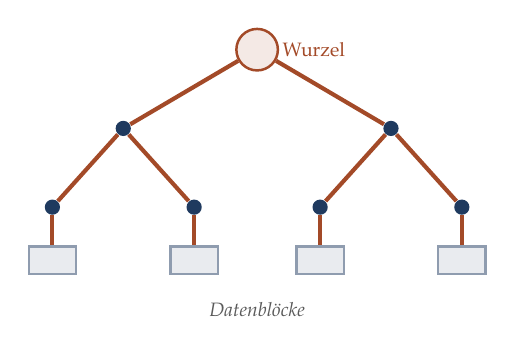
\begin{tikzpicture}[scale=1.0]
\node[knotenr] (w) at (0,2.1) {};
\node[knoten] (a) at (-1.7,1.1) {}; \node[knoten] (b) at (1.7,1.1) {};
\node[knoten] (a1) at (-2.6,0.1) {}; \node[knoten] (a2) at (-0.8,0.1) {};
\node[knoten] (b1) at (0.8,0.1) {}; \node[knoten] (b2) at (2.6,0.1) {};
\draw[kanted] (w)--(a); \draw[kanted] (w)--(b);
\draw[kanted] (a)--(a1); \draw[kanted] (a)--(a2);
\draw[kanted] (b)--(b1); \draw[kanted] (b)--(b2);
\foreach \x in {-2.6,-0.8,0.8,2.6}
  \draw[tief!50, line width=0.8pt, fill=tief!10] (\x-0.3,-0.75) rectangle ++(0.6,0.35);
\foreach \x in {-2.6,-0.8,0.8,2.6}
  \draw[kanted] (\x,0.0) -- (\x,-0.38);
\node[font=\scriptsize, color=akzent, anchor=west] at (0.2,2.1) {Wurzel};
\node[font=\scriptsize\itshape, color=grau] at (0,-1.2) {Datenblöcke};
\end{tikzpicture}
\end{center}

\schritt{Was das leistet}
Um zu belegen, dass ein bestimmter Block zum Ganzen gehört, genügen die Hashwerte entlang des Weges zur Wurzel.

\begin{center}
\renewcommand{\arraystretch}{1.48}
\begin{tabular}{@{}P{2.4cm}P{2.4cm}P{2.6cm}@{}}
\toprule
\textbf{Blöcke} & \textbf{Nachweis} & \\
\midrule
$1000$ & $10$ Hashwerte & \\
$10^{6}$ & $20$ Hashwerte & \\
$10^{9}$ & $30$ Hashwerte & \\
\bottomrule
\end{tabular}
\end{center}

\begin{center}
\begin{minipage}{0.88\textwidth}
\kursiv{Bei einer Milliarde Blöcken genügen dreißig Hashwerte --- knapp ein Kilobyte. \textbf{Die Nachweislänge wächst logarithmisch}, und darauf beruhen Versionsverwaltungen, verteilte Dateisysteme und die Blockketten der Kryptowährungen.}
\end{minipage}
\end{center}
\end{merksatz}

\section{Der Bruchfall}

\begin{warnung}
\boxtitelr{Was Hashfunktionen nicht leisten}
\begin{center}
{\small
\renewcommand{\arraystretch}{1.52}
\begin{tabular}{@{}P{2.4cm}P{6.2cm}@{}}
\toprule
\textbf{Keine Geheimhaltung} & Bei kleinem Wertebereich lässt sich das Urbild durch Ausprobieren finden. Ein Hashwert einer Patientennummer schützt sie nicht.\\
\textbf{Keine Beweise} & Kein praktisch verwendetes Verfahren hat einen Sicherheitsbeweis. Man vertraut auf gescheiterte Angriffsversuche.\\
\textbf{Vergleich in gleicher Zeit} & Ein Vergleich, der beim ersten Unterschied abbricht, verrät über die Laufzeit, wie viele Stellen stimmten.\\
\bottomrule
\end{tabular}}
\end{center}

\schritt{Zur ersten Zeile}
Eine Patientennummer aus acht Ziffern hat $10^{8}$ mögliche Werte.

\begin{center}
\begin{minipage}{0.9\textwidth}
\textbf{Das sind in Sekundenbruchteilen durchprobiert.} Der Hashwert ist dann kein Schutz, sondern eine umkehrbare Abbildung.
\end{minipage}
\end{center}

\begin{center}
\begin{minipage}{0.88\textwidth}
\kursiv{Dieser Fehler ist verbreitet: Man hält für anonymisiert, was nur gehasht ist. \textbf{Eine Hashfunktion verbirgt nur, was genug Entropie hat} --- und die Entropie einer Patientennummer beträgt knapp $27$ Bit. Wer anonymisieren will, braucht einen geheimen Schlüssel im Spiel, also einen Beglaubigungscode statt einer Hashfunktion.}
\end{minipage}
\end{center}

\schritt{Zur dritten Zeile}
\begin{center}
\begin{minipage}{0.88\textwidth}
\kursiv{Vergleicht man den erwarteten mit dem empfangenen Beglaubigungscode Byte für Byte und bricht beim ersten Unterschied ab, so dauert der Vergleich umso länger, je mehr Anfangsbytes stimmen. Ein Angreifer kann den Code dadurch Byte für Byte erraten --- statt $2^{128}$ Versuchen braucht er $16\cdot256$. \textbf{Ein korrektes Verfahren, falsch verglichen, ist kein Verfahren.}}
\end{minipage}
\end{center}
\end{warnung}

\section{Übungsaufgaben}

\begin{aufgabe}
\boxtitel{Aufgabe 11.1 --- Die Geburtstagsschranke anwenden}
Ein System vergibt zufällige Kennungen von $64$ Bit.
\begin{center}
{\small
\renewcommand{\arraystretch}{1.4}
\begin{tabular}{@{}P{0.8cm}P{7.6cm}@{}}
\toprule
(a) & Nach wie vielen Kennungen ist eine Doppelvergabe wahrscheinlicher als nicht?\\
(b) & Wie groß ist die Wahrscheinlichkeit bei einer Milliarde Kennungen?\\
(c) & Wie lang müssten die Kennungen sein, damit bei $10^{12}$ Vergaben die Wahrscheinlichkeit unter $10^{-9}$ bleibt?\\
\bottomrule
\end{tabular}}
\end{center}

\loesung
\schritt{(a)}
\[ k \approx 1{,}177\cdot2^{32} = 1{,}177\cdot4{,}29\cdot10^{9} = 5{,}06\cdot10^{9} \]

\begin{center}
\begin{minipage}{0.9\textwidth}
\textbf{Rund fünf Milliarden.}
\end{minipage}
\end{center}

\schritt{(b)}
\[ \Pr \approx 1-e^{-k^{2}/(2N)} = 1-\exp\left(-\frac{(10^{9})^{2}}{2\cdot1{,}845\cdot10^{19}}\right) \]
\[ = 1-\exp(-0{,}0271) = 0{,}0267 \]

\begin{center}
\begin{minipage}{0.9\textwidth}
\textbf{Etwa $2{,}7$ Prozent} --- bei einer Milliarde Kennungen aus $64$ Bit.
\end{minipage}
\end{center}

\begin{center}
\begin{minipage}{0.86\textwidth}
\kursiv{Das ist mehr, als die meisten erwarten. Eine Milliarde ist gegenüber $1{,}8\cdot10^{19}$ verschwindend --- und doch liegt die Kollisionswahrscheinlichkeit im Prozentbereich. Die Quadrierung im Exponenten ist der Grund.}
\end{minipage}
\end{center}

\schritt{(c)}
Für kleine Wahrscheinlichkeiten gilt
\[ \Pr \approx \frac{k^{2}}{2N} \quad\Longrightarrow\quad N \ \ge\ \frac{k^{2}}{2\Pr} \]

\[ N \ \ge\ \frac{(10^{12})^{2}}{2\cdot10^{-9}} = \frac{10^{24}}{2\cdot10^{-9}} = 5\cdot10^{32} \]

\[ n \ \ge\ \lb(5\cdot10^{32}) = 108{,}6 \]

\begin{center}
\begin{minipage}{0.9\textwidth}
\textbf{Mindestens $109$ Bit --- in der Praxis wählt man $128$.}
\end{minipage}
\end{center}

\schritt{Die Merkregel}
\begin{center}
\begin{minipage}{0.88\textwidth}
\kursiv{Für eine Kollisionswahrscheinlichkeit unter $2^{-t}$ bei $2^{m}$ Vergaben braucht man etwa $2m+t$ Bit. Hier: $2\cdot40 + 30 = 110$. \checkmark \textbf{Die Faustregel \enquote{doppelt so viele Bit wie Vergaben, plus Sicherheitsabstand} deckt alle Fälle ab.}}
\end{minipage}
\end{center}
\end{aufgabe}

\begin{aufgabe}
\boxtitel{Aufgabe 11.2 --- Die Längenerweiterung}
Ein System beglaubigt Befehle mit $t = H(K\Vert M)$. Der Angreifer kennt
\[ M = \texttt{"loesche=nein"}, \qquad t = H(K\Vert M) . \]
Was kann er erreichen, ohne $K$ zu kennen?

\loesung
\schritt{Schritt 1 --- Was der Angreifer weiß}
\begin{center}
{\small
\renewcommand{\arraystretch}{1.48}
\begin{tabular}{@{}P{2.4cm}P{2.6cm}P{2.6cm}@{}}
\toprule
\textbf{Größe} & \textbf{bekannt?} & \\
\midrule
$M$ & ja & abgehört\\
$t$ & ja & abgehört\\
$K$ & \textcolor{gruen}{nein} & \\
$|K|$ & meist ja & Systemangabe\\
\bottomrule
\end{tabular}}
\end{center}

\schritt{Schritt 2 --- Der Angriff}
Die Hashfunktion verarbeitet Blöcke und führt einen Zustand mit; $t$ ist der Endzustand.

\begin{center}
\renewcommand{\arraystretch}{1.5}
\begin{tabular}{@{}P{1.0cm}P{7.4cm}@{}}
\toprule
$1$ & Setze den internen Zustand auf $t$.\\
$2$ & Verarbeite den Anhang $M' = \texttt{"\&loesche=ja"}$.\\
$3$ & Gib den neuen Zustand als $t'$ aus.\\
\bottomrule
\end{tabular}
\end{center}

\schritt{Schritt 3 --- Das Ergebnis}
\[ t' = H\bigl(K \Vert M \Vert \text{Auffüllung} \Vert M'\bigr) \]

\begin{center}
\begin{minipage}{0.9\textwidth}
\textbf{Der Angreifer hat einen gültigen Beglaubigungscode für eine Nachricht erzeugt, die er sich ausgesucht hat.}
\end{minipage}
\end{center}

\schritt{Schritt 4 --- Was der Empfänger sieht}
\begin{center}
{\small
\renewcommand{\arraystretch}{1.48}
\begin{tabular}{@{}P{2.8cm}P{5.4cm}@{}}
\toprule
\textbf{Nachricht} & \texttt{loesche=nein}, Füllbytes, \texttt{\&loesche=ja}\\
\textbf{Code} & gültig\\
\bottomrule
\end{tabular}}
\end{center}

\begin{center}
\begin{minipage}{0.88\textwidth}
\kursiv{Ob die Füllbytes stören, hängt vom Empfänger ab. Viele Auswerteverfahren überlesen unbekannte Zeichen oder werten bei doppelten Angaben die \kursiv{letzte} aus --- und dann steht dort \texttt{ja}. \textbf{Die Schwäche der Hashfunktion und die Nachlässigkeit des Auswerters wirken zusammen}, und beide für sich wären harmloser.}
\end{minipage}
\end{center}

\schritt{Schritt 5 --- Drei Abhilfen}
\begin{center}
{\small
\renewcommand{\arraystretch}{1.5}
\begin{tabular}{@{}P{2.4cm}P{6.2cm}@{}}
\toprule
\textbf{HMAC} & Zweifache Anwendung; der äußere Aufruf verdeckt den inneren Zustand.\\
\textbf{Schwamm-Funktion} & Gibt nur einen Teil des Zustands aus; die Fortsetzung ist unmöglich.\\
\textbf{Schlüssel hinten} & $H(M\Vert K)$ vermeidet die Längenerweiterung --- ist aber gegen Kollisionen in $H$ anfällig.\\
\bottomrule
\end{tabular}}
\end{center}

\begin{center}
\begin{minipage}{0.88\textwidth}
\kursiv{Die dritte Zeile zeigt, warum man solche Konstruktionen nicht selbst entwerfen sollte: Jede naheliegende Variante hat eine eigene Schwäche. \textbf{HMAC ist nicht deshalb Standard, weil es elegant wäre, sondern weil es bewiesen ist} --- und weil die Alternativen einzeln geprüft und verworfen wurden.}
\end{minipage}
\end{center}
\end{aufgabe}

\begin{aufgabe}
\boxtitel{Aufgabe 11.3 --- Passwörter}
Eine Klinik speichert $5000$ Passwortwerte. Vergleichen Sie drei Verfahren gegen einen Angreifer, der die Datei erbeutet hat und $10^{10}$ Hashwerte je Sekunde berechnen kann.

\loesung
\schritt{Schritt 1 --- Die Annahmen}
Passwörter aus acht Zeichen von $94$ möglichen:
\[ 94^{8} = 6{,}1\cdot10^{15} \]

\schritt{Schritt 2 --- Schnelle Hashfunktion ohne Salz}
Der Angreifer berechnet einmal alle Hashwerte und vergleicht mit \kursiv{allen} $5000$ Einträgen zugleich.
\[ \frac{6{,}1\cdot10^{15}}{10^{10}} = 6{,}1\cdot10^{5} \ \text{Sekunden} = 7{,}1 \ \text{Tage} \]

\begin{center}
\begin{minipage}{0.9\textwidth}
\textbf{Sieben Tage für \kursiv{alle} fünftausend Passwörter.} Der Aufwand hängt nicht von ihrer Zahl ab.
\end{minipage}
\end{center}

\schritt{Schritt 3 --- Schnelle Hashfunktion mit Salz}
Jeder Eintrag hat ein eigenes Salz; der Angreifer muss jedes Passwort einzeln angreifen.
\[ 5000 \cdot 7{,}1 \ \text{Tage} = 35\,500 \ \text{Tage} = 97 \ \text{Jahre} \]

\begin{center}
\begin{minipage}{0.9\textwidth}
\textbf{Das Salz verwandelt einen Angriff auf alle in fünftausend Einzelangriffe.}
\end{minipage}
\end{center}

\begin{center}
\begin{minipage}{0.86\textwidth}
\kursiv{Auf \kursiv{ein} bestimmtes Passwort dauert es weiterhin sieben Tage. Das Salz schützt also die Menge, nicht den Einzelnen --- und genau deshalb braucht es zusätzlich die dritte Maßnahme.}
\end{minipage}
\end{center}

\schritt{Schritt 4 --- Langsame Funktion mit Salz}
Bei $10^{4}$ Berechnungen je Sekunde:
\[ \frac{6{,}1\cdot10^{15}}{10^{4}} = 6{,}1\cdot10^{11} \ \text{Sekunden} = 19\,400 \ \text{Jahre} \]

\begin{center}
\begin{minipage}{0.9\textwidth}
\textbf{Neunzehntausend Jahre für ein einziges Passwort.}
\end{minipage}
\end{center}

\schritt{Schritt 5 --- Die Übersicht}
\begin{center}
{\small
\renewcommand{\arraystretch}{1.48}
\begin{tabular}{@{}P{2.6cm}P{2.4cm}P{2.6cm}@{}}
\toprule
\textbf{Verfahren} & \textbf{alle $5000$} & \textbf{ein einzelnes}\\
\midrule
schnell, ohne Salz & $7$ Tage & $7$ Tage\\
schnell, mit Salz & $97$ Jahre & $7$ Tage\\
langsam, mit Salz & --- & $\mathbf{19\,400}$ \textbf{Jahre}\\
\bottomrule
\end{tabular}}
\end{center}

\schritt{Schritt 6 --- Der entscheidende Vorbehalt}
Die Rechnung unterstellt, dass die Passwörter gleichverteilt aus $94^{8}$ gewählt sind.

\begin{center}
\begin{minipage}{0.9\textwidth}
\textbf{Tatsächlich haben von Menschen gewählte Passwörter eine Entropie von etwa $20$ bis $30$ Bit --- nicht $52$.}
\end{minipage}
\end{center}

\begin{center}
\begin{minipage}{0.88\textwidth}
\kursiv{Bei $25$ Bit sind es $3{,}4\cdot10^{7}$ Möglichkeiten; selbst bei $10^{4}$ Versuchen je Sekunde ist das in einer Stunde durchprobiert. \textbf{Die Entropie des Passworts ist die eigentliche Schranke} --- alle Maßnahmen dieses Abschnitts vergrößern nur den Aufwand je Versuch, nicht die Zahl der Möglichkeiten. Das ist genau die Aussage von Satz 9.3 in anderer Gestalt: Ohne genug Entropie hilft kein Verfahren.}
\end{minipage}
\end{center}
\end{aufgabe}

\begin{geschichte}
\boxtitelg{Zwei Funktionen, zwei Jahrzehnte}
\Person{Ronald Rivest} entwarf 1991 die Funktion MD5 als Nachfolgerin von MD4, gegen die bereits Angriffe bekannt waren.

\begin{center}
\begin{minipage}{0.9\textwidth}
\kursiv{MD5 wurde binnen weniger Jahre allgegenwärtig --- in Zertifikaten, Signaturen, Dateiprüfsummen, Passwortspeichern. 1996 fand \Person{Hans Dobbertin} eine Kollision der inneren Kompressionsfunktion und riet öffentlich von weiterer Verwendung ab. Es geschah wenig.}
\end{minipage}
\end{center}

\schritt{Der Bruch}
2004 stellte \Person{Wang Xiaoyun} auf einer Konferenz vollständige Kollisionen vor --- berechnet in etwa einer Stunde.

\begin{center}
\begin{minipage}{0.9\textwidth}
\kursiv{Die Arbeit kam überraschend und traf zugleich MD4, MD5, RIPEMD und HAVAL. Wangs Verfahren beruhte auf einer sorgfältigen Analyse der Differenzenfortpflanzung, die im Westen so nicht verfolgt worden war. \textbf{Heute dauert eine MD5-Kollision Sekundenbruchteile}, und die Funktion gilt seit zwanzig Jahren als gebrochen --- wird aber weiterhin in Altsystemen angetroffen.}
\end{minipage}
\end{center}

\schritt{SHA-1}
1995 als Norm verabschiedet, mit $160$ Bit. Ab 2005 zeigten Wang und andere theoretische Angriffe unter $2^{80}$.

\begin{center}
\begin{minipage}{0.9\textwidth}
\kursiv{2017 gelang einer Arbeitsgruppe bei Google die erste vollständige Kollision --- zwei PDF-Dateien mit gleichem Hashwert und verschiedenem Inhalt. Der Aufwand betrug etwa $2^{63}$ Rechenschritte, umgerechnet einige zehntausend Jahre auf einem einzelnen Rechenkern. \textbf{Zwischen der ersten Warnung und dem praktischen Nachweis lagen zwölf Jahre} --- und dazwischen die zähe Umstellung ganzer Infrastrukturen.}
\end{minipage}
\end{center}

\schritt{Der Wettbewerb}
2007 schrieb das amerikanische Normungsinstitut einen offenen Wettbewerb aus --- nach dem Vorbild aus Kapitel~10.

\begin{center}
\begin{minipage}{0.9\textwidth}
\kursiv{2012 gewann Keccak von \Person{Guido Bertoni}, \Person{Joan Daemen} --- demselben wie bei Rijndael ---, \Person{Michaël Peeters} und \Person{Gilles Van Assche}. Die Schwammbauweise unterscheidet sich grundlegend von der bisherigen und macht die Längenerweiterung strukturell unmöglich. \textbf{Der Wettbewerb wurde begonnen, bevor SHA-2 gebrochen war} --- und das ist die eigentliche Lehre: Man baut den Nachfolger, solange noch Zeit ist.}
\end{minipage}
\end{center}
\end{geschichte}

\begin{forschung}
\boxtitelp{Hashfunktionen heute}
\begin{center}
{\small
\renewcommand{\arraystretch}{1.45}
\begin{tabular}{@{}P{2.8cm}P{5.4cm}@{}}
\toprule
\textbf{Stand} & SHA-2 und SHA-3 gelten als sicher; die besten Angriffe erreichen nur stark verkürzte Rundenzahlen.\\
\textbf{Passwort\-funktionen} & Verfahren, die absichtlich viel Speicher brauchen --- gegen Spezialhardware.\\
\textbf{Nachweisbarkeit} & Hashbäume als Grundlage für Belege, die sich nicht nachträglich ändern lassen.\\
\bottomrule
\end{tabular}}
\end{center}

\schritt{Zur zweiten Zeile}
Spezialhardware kann Hashwerte millionenfach schneller berechnen als Standardrechner --- aber Speicher lässt sich nicht ebenso vervielfachen.

\begin{center}
\begin{minipage}{0.88\textwidth}
\kursiv{Deshalb sind moderne Passwortfunktionen so gebaut, dass sie einige hundert Megabyte Arbeitsspeicher benötigen. Das verteuert Spezialhardware erheblich und gleicht den Vorteil des Angreifers aus. \textbf{Man verlagert den Wettbewerb von einer Größe, bei der der Angreifer im Vorteil ist, auf eine, bei der er es nicht ist} --- eine Denkweise, die auch außerhalb der Kryptographie nützlich wäre.}
\end{minipage}
\end{center}

\schritt{Und die Quantenfrage}
Grovers Verfahren halbiert den Exponenten bei der Urbildsuche: aus $2^{n}$ wird $2^{n/2}$.

\begin{center}
\begin{minipage}{0.88\textwidth}
\kursiv{Für Kollisionen ist der Gewinn geringer und nach heutigem Stand praktisch bedeutungslos. \textbf{Hashfunktionen sind die am wenigsten bedrohte Bausteinfamilie}: Eine Verdopplung der Ausgabelänge genügt als Vorsorge. Für die Verfahren aus Teil~V sieht das völlig anders aus --- Kapitel~15.}
\end{minipage}
\end{center}
\end{forschung}

\begin{merksatz}
\boxtitel{Was Sie jetzt können}
\begin{center}
\renewcommand{\arraystretch}{1.5}
\begin{tabular}{@{}P{3.4cm}P{5.2cm}@{}}
\toprule
\textbf{Definition 11.1} & drei Anforderungen, zwei Aufwände\\
\textbf{Satz 11.2} & $k \approx 1{,}177\sqrt N$\\
\textbf{Längen\-erweiterung} & warum $H(K\Vert M)$ falsch ist\\
\textbf{Salz und Langsamkeit} & sieben Tage gegen $19\,000$ Jahre\\
\textbf{Hashbäume} & Nachweis in $\lb n$ Werten\\
\bottomrule
\end{tabular}
\end{center}

\begin{center}
\begin{minipage}{0.88\textwidth}
\kursiv{Damit endet Teil~IV. Alle bisherigen Verfahren setzen einen gemeinsamen Schlüssel voraus. Ab Kapitel~12 fragen wir, wie zwei Fremde einen solchen vereinbaren können --- über eine abgehörte Leitung.}
\end{minipage}
\end{center}
\end{merksatz}

\part{Öffentliche Schlüssel}

\chapter{Schlüsseltausch über offene Leitung}

\section{Das Problem}

\begin{merksatz}
\boxtitel{Was alle bisherigen Verfahren voraussetzen}
\begin{center}
{\small
\renewcommand{\arraystretch}{1.5}
\begin{tabular}{@{}P{2.4cm}P{6.2cm}@{}}
\toprule
\textbf{Kapitel 9} & Sender und Empfänger teilen einen Einmalschlüssel.\\
\textbf{Kapitel 10} & Sie teilen einen Blockchiffrenschlüssel.\\
\textbf{Kapitel 11} & Sie teilen einen Beglaubigungsschlüssel.\\
\bottomrule
\end{tabular}}
\end{center}

\begin{center}
\begin{minipage}{0.9\textwidth}
\textbf{Woher kommt dieser gemeinsame Schlüssel?}
\end{minipage}
\end{center}

\schritt{Das Ausmaß des Problems}
Bei $n$ Teilnehmern, die paarweise vertraulich kommunizieren wollen, braucht man
\[ \binom{n}{2} = \frac{n(n-1)}{2} \ \text{Schlüssel.} \]

\begin{center}
{\small
\renewcommand{\arraystretch}{1.48}
\begin{tabular}{@{}P{2.4cm}P{2.4cm}P{2.6cm}@{}}
\toprule
\textbf{Teilnehmer} & \textbf{Schlüssel} & \\
\midrule
$10$ & $45$ & Praxisnetz\\
$1000$ & $499\,500$ & Klinikverbund\\
$10^{6}$ & $5\cdot10^{11}$ & \textcolor{akzent}{aussichtslos}\\
\bottomrule
\end{tabular}}
\end{center}

\begin{center}
\begin{minipage}{0.88\textwidth}
\kursiv{Und jeder einzelne müsste persönlich oder per Kurier übergeben werden. \textbf{Bis 1976 galt das als grundsätzliche Grenze der Kryptographie} --- man könne ohne vorherigen sicheren Kanal keinen Schlüssel vereinbaren. Der Gedanke, dass es anders geht, kam erst spät und wirkte zunächst unglaubwürdig.}
\end{minipage}
\end{center}
\end{merksatz}

\section{Rechnen mit Resten}

\begin{merksatz}
\boxtitel{Das Nötige in Kürze}
Für eine Primzahl $p$ rechnet man mit den Resten $1,2,\ldots,p-1$ bei Division durch $p$.

\begin{center}
{\small
\renewcommand{\arraystretch}{1.5}
\begin{tabular}{@{}P{2.8cm}P{5.8cm}@{}}
\toprule
\textbf{Multiplikation} & $a\cdot b \bmod p$ bleibt im Bereich.\\
\textbf{Umkehrbarkeit} & Zu jedem $a \ne 0$ gibt es genau ein $a^{-1}$ mit $a\,a^{-1} \equiv 1$.\\
\textbf{Kleiner Satz von Fermat} & $a^{p-1} \equiv 1$ für alle $a \ne 0$.\\
\bottomrule
\end{tabular}}
\end{center}

\schritt{Die Primitivwurzel}
Ein Element $g$ heißt \Begriff{Primitivwurzel}, wenn seine Potenzen alle Reste durchlaufen:
\[ \{g^1, g^2, \ldots, g^{p-1}\} = \{1,2,\ldots,p-1\} \]

\kursiv{Beispiel:} $p=23$, $g=5$.
\begin{center}
{\small
\renewcommand{\arraystretch}{1.4}
\begin{tabular}{@{}P{0.9cm}P{0.9cm}P{0.9cm}P{0.9cm}P{0.9cm}P{0.9cm}P{0.9cm}P{0.9cm}@{}}
\toprule
$k$ & $1$ & $2$ & $3$ & $4$ & $5$ & $6$ & $7$\\
$5^k$ & $5$ & $2$ & $10$ & $4$ & $20$ & $\mathbf{8}$ & $17$\\
\midrule
$k$ & $8$ & $9$ & $10$ & $11$ & $\cdots$ & $21$ & $22$\\
$5^k$ & $16$ & $11$ & $9$ & $22$ & $\cdots$ & $14$ & $1$\\
\bottomrule
\end{tabular}}
\end{center}

Alle $22$ Werte sind verschieden --- $5$ ist eine Primitivwurzel modulo $23$.

\begin{center}
\begin{minipage}{0.88\textwidth}
\kursiv{Dass es solche Elemente gibt, ist ein Satz der Zahlentheorie: Die multiplikative Gruppe modulo einer Primzahl ist zyklisch. Der Beweis steht in Band 8, Teil~III. \textbf{Für dieses Kapitel genügt die Tatsache}, und sie lässt sich an jedem Beispiel nachprüfen.}
\end{minipage}
\end{center}
\end{merksatz}

\begin{merksatz}
\boxtitel{Potenzieren ist schnell}
Die Berechnung von $g^{a} \bmod p$ erfordert nicht $a$ Multiplikationen, sondern nur etwa $2\lb a$.

\schritt{Quadrieren und Multiplizieren}
Man liest den Exponenten binär von links und rechnet fortlaufend:
\begin{center}
\renewcommand{\arraystretch}{1.5}
\begin{tabular}{@{}P{2.0cm}P{6.6cm}@{}}
\toprule
\textbf{Bit $0$} & quadrieren\\
\textbf{Bit $1$} & quadrieren, dann mit $g$ multiplizieren\\
\bottomrule
\end{tabular}
\end{center}

\kursiv{Beispiel:} $5^{15} \bmod 23$ mit $15 = \texttt{1111}_2$:
\begin{center}
\renewcommand{\arraystretch}{1.46}
\begin{tabular}{@{}P{1.4cm}P{2.6cm}P{2.4cm}@{}}
\toprule
\textbf{Bit} & \textbf{Rechnung} & \textbf{Ergebnis}\\
\midrule
$1$ & $1^2\cdot5$ & $5$\\
$1$ & $5^2\cdot5 = 125$ & $10$\\
$1$ & $10^2\cdot5 = 500$ & $17$\\
$1$ & $17^2\cdot5 = 1445$ & $\mathbf{19}$\\
\bottomrule
\end{tabular}
\end{center}

\kursiv{Probe:} $125 = 5\cdot23+10$ \checkmark; $500 = 21\cdot23+17$ \checkmark; $1445 = 62\cdot23+19$ \checkmark

\begin{center}
\begin{minipage}{0.9\textwidth}
\textbf{Vier Schritte statt fünfzehn.} Bei einem Exponenten von $2048$ Bit sind es rund $3000$ statt $10^{616}$.
\end{minipage}
\end{center}

\begin{center}
\begin{minipage}{0.88\textwidth}
\kursiv{Genau auf diesem Gefälle beruht das ganze Kapitel: \textbf{Potenzieren ist leicht, der umgekehrte Weg vermutlich schwer.} Eine Funktion mit dieser Eigenschaft nennt man eine Einwegfunktion.}
\end{minipage}
\end{center}
\end{merksatz}

\section{Das Verfahren}

\begin{merksatz}
\boxtitel{Diffie-Hellman-Schlüsseltausch}
Öffentlich bekannt sind $p$ und eine Primitivwurzel $g$.

\begin{center}
{\small
\renewcommand{\arraystretch}{1.55}
\begin{tabular}{@{}P{2.4cm}P{2.6cm}P{3.0cm}@{}}
\toprule
\textbf{Schritt} & \textbf{Alice} & \textbf{Bob}\\
\midrule
$1$ & wählt $a$ geheim & wählt $b$ geheim\\
$2$ & sendet $A = g^{a}$ & sendet $B = g^{b}$\\
$3$ & rechnet $B^{a}$ & rechnet $A^{b}$\\
\bottomrule
\end{tabular}}
\end{center}

\schritt{Warum beide dasselbe erhalten}
\[ B^{a} = (g^{b})^{a} = g^{ab} = (g^{a})^{b} = A^{b} \]

\begin{center}
\begin{minipage}{0.9\textwidth}
\textbf{Das Potenzgesetz ist der ganze Trick.} Die Reihenfolge der Exponenten spielt keine Rolle.
\end{minipage}
\end{center}

\schritt{Ein vollständiges Beispiel}
$p=23$, $g=5$, $a=6$, $b=15$.

\begin{center}
{\small
\renewcommand{\arraystretch}{1.48}
\begin{tabular}{@{}P{2.2cm}P{2.8cm}P{2.8cm}@{}}
\toprule
& \textbf{Alice} & \textbf{Bob}\\
\midrule
geheim & $a = 6$ & $b = 15$\\
gesendet & $A = 5^{6} = 8$ & $B = 5^{15} = 19$\\
gerechnet & $19^{6} = \mathbf{2}$ & $8^{15} = \mathbf{2}$\\
\bottomrule
\end{tabular}}
\end{center}

\kursiv{Probe:} $g^{ab} = 5^{90} \bmod 23$. Wegen $5^{22}\equiv1$ und $90 = 4\cdot22+2$ ist $5^{90} \equiv 5^{2} = 25 \equiv 2$. \checkmark

\schritt{Was der Mitleser sieht}
\[ p = 23, \quad g = 5, \quad A = 8, \quad B = 19 \]

\begin{center}
\begin{minipage}{0.9\textwidth}
\textbf{Er kennt $g^{a}$ und $g^{b}$ und will $g^{ab}$.} Dafür müsste er $a$ oder $b$ bestimmen.
\end{minipage}
\end{center}
\end{merksatz}

\begin{definition}
\boxtitelm{Definition 12.1 --- das diskrete Logarithmusproblem}
Gegeben $p$, $g$ und $y$, bestimme $x$ mit
\[ g^{x} \equiv y \pmod p . \]
\end{definition}

\begin{merksatz}
\boxtitel{Der Stand}
\begin{center}
\begin{minipage}{0.9\textwidth}
\textbf{Für große Primzahlen ist kein Verfahren bekannt, das dieses Problem in vertretbarer Zeit löst.} Bewiesen ist die Schwierigkeit nicht.
\end{minipage}
\end{center}

\begin{center}
\begin{minipage}{0.88\textwidth}
\kursiv{Es ist dieselbe Lage wie bei $\mathsf{P}$ gegen $\mathsf{NP}$ in Band 19: Man weiß nicht, ob es schwer ist, sondern nur, dass seit fünfzig Jahren niemand einen schnellen Weg gefunden hat. \textbf{Die dritte Warnung aus dem Vorwort steht hier zum ersten Mal in voller Schärfe.}}
\end{minipage}
\end{center}

\schritt{Ein feiner Unterschied}
Streng genommen muss der Angreifer nicht den Logarithmus bestimmen --- er braucht nur $g^{ab}$.

\begin{center}
{\small
\renewcommand{\arraystretch}{1.5}
\begin{tabular}{@{}P{3.4cm}P{5.2cm}@{}}
\toprule
\textbf{Logarithmus\-problem} & Aus $g^{a}$ bestimme $a$.\\
\textbf{Diffie-Hellman-Problem} & Aus $g^{a}$ und $g^{b}$ bestimme $g^{ab}$.\\
\bottomrule
\end{tabular}}
\end{center}

\begin{center}
\begin{minipage}{0.88\textwidth}
\kursiv{Das zweite ist höchstens so schwer wie das erste --- wer Logarithmen ziehen kann, löst auch das zweite. Ob es \kursiv{genauso} schwer ist, ist offen. Für die meisten Gruppen vermutet man es; bewiesen ist es nur unter Zusatzannahmen. \textbf{Die Sicherheit des Verfahrens beruht auf einer Annahme, die schwächer ist als die naheliegende} --- und das wird oft übersehen.}
\end{minipage}
\end{center}
\end{merksatz}

\section{Wie schwer ist es wirklich}

\begin{merksatz}
\boxtitel{Drei Angriffsverfahren}
\begin{center}
{\small
\renewcommand{\arraystretch}{1.52}
\begin{tabular}{@{}P{2.8cm}P{2.4cm}P{2.8cm}@{}}
\toprule
\textbf{Verfahren} & \textbf{Aufwand} & \textbf{Speicher}\\
\midrule
Durchprobieren & $p$ & $O(1)$\\
Riesen- und Zwergenschritte & $\sqrt p$ & $\sqrt p$\\
Pollards Rho & $\sqrt p$ & $O(1)$\\
\textbf{Indexrechnung} & \textcolor{akzent}{unter\-exponentiell} & groß\\
\bottomrule
\end{tabular}}
\end{center}

\schritt{Riesen- und Zwergenschritte}
Man schreibt $x = i\,m + j$ mit $m = \lceil\sqrt{p-1}\rceil$ und $0 \le j < m$:
\[ g^{x} = y \quad\Longleftrightarrow\quad g^{j} = y\cdot(g^{-m})^{i} \]

\begin{center}
\renewcommand{\arraystretch}{1.5}
\begin{tabular}{@{}P{1.0cm}P{7.4cm}@{}}
\toprule
$1$ & Tabelliere $g^{j}$ für $j = 0,\ldots,m-1$ (die Zwergenschritte).\\
$2$ & Berechne $y\cdot(g^{-m})^{i}$ für $i = 0,1,\ldots$ (die Riesenschritte).\\
$3$ & Bei einem Treffer ist $x = i\,m+j$.\\
\bottomrule
\end{tabular}
\end{center}

\kursiv{Beispiel:} $p=23$, $g=5$, $y=8$. Mit $m=5$:
\begin{center}
\renewcommand{\arraystretch}{1.46}
\begin{tabular}{@{}P{1.2cm}P{1.2cm}P{1.2cm}P{1.2cm}P{1.2cm}@{}}
\toprule
$j$ & $0$ & $1$ & $2$ & $3$\\
$5^j$ & $1$ & $\mathbf{5}$ & $2$ & $10$\\
\bottomrule
\end{tabular}
\end{center}

\kursiv{Riesenschritt $i=1$:} $8\cdot(5^{-5}) \bmod 23 = 5$ --- Treffer bei $j=1$.
\[ x = 1\cdot5 + 1 = 6 \quad \checkmark \]

\begin{center}
\begin{minipage}{0.88\textwidth}
\kursiv{Statt $22$ Versuchen genügen $5+2 = 7$. Bei $p \approx 2^{2048}$ wären es $2^{1024}$ --- immer noch aussichtslos. \textbf{Die Wurzel halbiert den Exponenten, und das genügt bei großen Zahlen nicht.}}
\end{minipage}
\end{center}
\end{merksatz}

\begin{warnung}
\boxtitelr{Die Indexrechnung ändert alles}
Für Restklassen modulo einer Primzahl gibt es ein Verfahren, dessen Aufwand langsamer wächst als jede Potenz --- aber schneller als jedes Polynom.

\[ L_p\!\left[\tfrac13,\,1{,}923\right] = \exp\left(1{,}923\,(\ln p)^{1/3}(\ln\ln p)^{2/3}\right) \]

\begin{center}
{\small
\renewcommand{\arraystretch}{1.48}
\begin{tabular}{@{}P{2.0cm}P{2.2cm}P{2.6cm}@{}}
\toprule
\textbf{Größe von $p$} & \textbf{Aufwand} & \\
\midrule
$2^{512}$ & $2^{63{,}9}$ & \textcolor{akzent}{gebrochen}\\
$2^{1024}$ & $2^{86{,}8}$ & \textcolor{mittel}{grenzwertig}\\
$2^{2048}$ & $2^{116{,}9}$ & sicher\\
$2^{3072}$ & $2^{138{,}7}$ & sicher\\
\bottomrule
\end{tabular}}
\end{center}

\begin{center}
\begin{minipage}{0.9\textwidth}
\textbf{Ein Schlüssel von $1024$ Bit bietet nur etwa $87$ Bit Sicherheit --- nicht $512$, wie die Wurzelschranke nahelegte.}
\end{minipage}
\end{center}

\begin{center}
\begin{minipage}{0.88\textwidth}
\kursiv{Das ist der Grund für die scheinbar übertriebenen Schlüssellängen: Man braucht $3072$ Bit, um die Sicherheit eines $128$-Bit-Blockchiffrenschlüssels zu erreichen. \textbf{Die Zahlen der beiden Welten sind nicht vergleichbar}, und das führt regelmäßig zu Fehleinschätzungen.}
\end{minipage}
\end{center}

\schritt{Warum elliptische Kurven kürzer sind}
Die Indexrechnung beruht auf der Zerlegung in Primfaktoren --- ein Begriff, den es in der Gruppe einer elliptischen Kurve nicht gibt.

\begin{center}
{\small
\renewcommand{\arraystretch}{1.48}
\begin{tabular}{@{}P{2.2cm}P{2.2cm}P{2.2cm}P{1.8cm}@{}}
\toprule
\textbf{Sicherheit} & \textbf{DH/RSA} & \textbf{elliptisch} & \textbf{Faktor}\\
\midrule
$80$ Bit & $1024$ & $160$ & $6{,}4$\\
$112$ Bit & $2048$ & $224$ & $9{,}1$\\
$128$ Bit & $3072$ & $256$ & $12{,}0$\\
$256$ Bit & $15\,360$ & $512$ & $\mathbf{30{,}0}$\\
\bottomrule
\end{tabular}}
\end{center}

\begin{center}
\begin{minipage}{0.88\textwidth}
\kursiv{Bei elliptischen Kurven ist die Wurzelschranke tatsächlich das Beste, was man kennt --- also $2^{n/2}$ bei $n$ Bit. \textbf{Der Vorteil wächst mit der geforderten Sicherheit}, und bei hohen Anforderungen ist er dreißigfach. Kapitel~14 behandelt diese Gruppen.}
\end{minipage}
\end{center}
\end{warnung}

\section{Der Bruchfall}

\begin{warnung}
\boxtitelr{Der Mann in der Mitte}
Das Verfahren sichert Vertraulichkeit --- nicht Herkunft.

\begin{center}
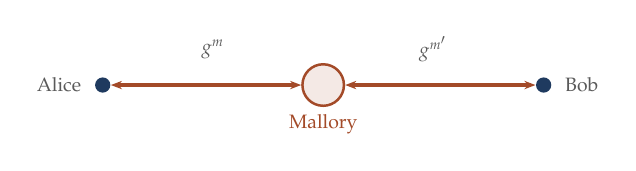
\begin{tikzpicture}[scale=1.0]
\node[knoten] (a) at (0,0) {}; \node[knotenr] (m) at (2.8,0) {}; \node[knoten] (b) at (5.6,0) {};
\draw[kanted, {Stealth[length=4pt]}-{Stealth[length=4pt]}] (a)--(m);
\draw[kanted, {Stealth[length=4pt]}-{Stealth[length=4pt]}] (m)--(b);
\node[font=\scriptsize, color=grau, anchor=east] at (-0.15,0) {Alice};
\node[font=\scriptsize, color=akzent, anchor=north] at (2.8,-0.25) {Mallory};
\node[font=\scriptsize, color=grau, anchor=west] at (5.75,0) {Bob};
\node[font=\scriptsize, color=grau] at (1.4,0.45) {$g^{m}$};
\node[font=\scriptsize, color=grau] at (4.2,0.45) {$g^{m'}$};
\end{tikzpicture}
\end{center}

\schritt{Der Ablauf}
\begin{center}
\renewcommand{\arraystretch}{1.5}
\begin{tabular}{@{}P{1.0cm}P{7.4cm}@{}}
\toprule
$1$ & Mallory fängt $A = g^{a}$ ab und sendet Bob stattdessen $g^{m}$.\\
$2$ & Ebenso in die Gegenrichtung.\\
$3$ & Alice teilt nun einen Schlüssel mit Mallory, Bob einen anderen.\\
$4$ & Mallory entschlüsselt, liest, verschlüsselt neu und leitet weiter.\\
\bottomrule
\end{tabular}
\end{center}

\begin{center}
\begin{minipage}{0.9\textwidth}
\textbf{Beide glauben, miteinander zu sprechen, und bemerken nichts.}
\end{minipage}
\end{center}

\begin{center}
\begin{minipage}{0.88\textwidth}
\kursiv{Der Angriff braucht keinerlei Rechenkraft --- er umgeht die Mathematik vollständig. \textbf{Der Schlüsseltausch löst genau eine Hälfte des Problems}, und die andere Hälfte erfordert, dass Alice weiß, welcher öffentliche Wert zu Bob gehört. Kapitel~14 behandelt Signaturen, Kapitel~15 die Frage, wie man einen öffentlichen Schlüssel überhaupt jemandem zuordnet.}
\end{minipage}
\end{center}
\end{warnung}

\begin{warnung}
\boxtitelr{Und drei weitere Fallen}
\begin{center}
{\small
\renewcommand{\arraystretch}{1.5}
\begin{tabular}{@{}P{2.4cm}P{6.2cm}@{}}
\toprule
\textbf{Kleine Untergruppen} & Ist $p-1$ in kleine Faktoren zerlegbar, so lässt sich das Problem in Teilprobleme zerlegen. Man wählt $p = 2q+1$ mit $q$ prim.\\
\textbf{Feste Parameter} & Wird dieselbe Primzahl von Millionen Systemen genutzt, so lohnt sich eine einmalige Vorberechnung.\\
\textbf{Schwache Exponenten} & Ein vorhersehbarer Zufallsgenerator macht $a$ ratbar --- die Mathematik ist dann gleichgültig.\\
\bottomrule
\end{tabular}}
\end{center}

\schritt{Zur zweiten Zeile}
Die Indexrechnung zerfällt in eine teure Vorberechnung, die nur von $p$ abhängt, und eine billige Endphase je Logarithmus.

\begin{center}
\begin{minipage}{0.88\textwidth}
\kursiv{Eine 2015 veröffentlichte Untersuchung zeigte, dass eine einzige $1024$-Bit-Primzahl von einem erheblichen Teil aller damaligen Verbindungen verwendet wurde. \textbf{Wer die Vorberechnung einmal leistet, bricht danach jede einzelne Verbindung binnen Minuten.} Der Aufwand lag in der Größenordnung dessen, was ein Staat aufbringen kann --- und die Verfasser hielten es für wahrscheinlich, dass es geschehen war.}
\end{minipage}
\end{center}
\end{warnung}

\section{Übungsaufgaben}

\begin{aufgabe}
\boxtitel{Aufgabe 12.1 --- Ein Schlüsseltausch von Hand}
Mit $p = 23$ und $g = 5$ wählt Alice $a = 4$ und Bob $b = 3$. Führen Sie den Tausch durch und prüfen Sie das Ergebnis.

\loesung
\schritt{Schritt 1 --- Alices Wert}
\[ A = 5^{4} = 625 \]
\[ 625 = 27\cdot23 + 4 \quad\Longrightarrow\quad A = 4 \]

\schritt{Schritt 2 --- Bobs Wert}
\[ B = 5^{3} = 125 = 5\cdot23+10 \quad\Longrightarrow\quad B = 10 \]

\schritt{Schritt 3 --- Alice rechnet}
\[ B^{a} = 10^{4} = 10\,000 \]
\kursiv{Schrittweise:} $10^2 = 100 = 4\cdot23+8$, also $8$. Dann $8^2 = 64 = 2\cdot23+18$, also $\mathbf{18}$.

\schritt{Schritt 4 --- Bob rechnet}
\[ A^{b} = 4^{3} = 64 = 2\cdot23+18 \quad\Longrightarrow\quad \mathbf{18} \]

\begin{center}
\begin{minipage}{0.9\textwidth}
\textbf{Beide erhalten $18$.} \checkmark
\end{minipage}
\end{center}

\schritt{Schritt 5 --- Die Probe}
\[ g^{ab} = 5^{12} \bmod 23 \]
Aus der Tabelle in Abschnitt 12.2: $5^{12} = 18$. \checkmark

\schritt{Schritt 6 --- Was der Mitleser tun müsste}
Er kennt $5$, $23$, $4$ und $10$. Um $a$ zu finden, probiert er:
\begin{center}
\renewcommand{\arraystretch}{1.44}
\begin{tabular}{@{}P{1.2cm}P{1.2cm}P{1.2cm}P{1.2cm}P{1.2cm}@{}}
\toprule
$k$ & $1$ & $2$ & $3$ & $4$\\
$5^k$ & $5$ & $2$ & $10$ & $\mathbf{4}$\\
\bottomrule
\end{tabular}
\end{center}

Nach vier Versuchen hat er $a=4$.

\begin{center}
\begin{minipage}{0.88\textwidth}
\kursiv{Bei $p=23$ ist das Verfahren wertlos --- es gibt nur $22$ Möglichkeiten. \textbf{Die Sicherheit entsteht ausschließlich aus der Größe}, und praktisch verwendet man Primzahlen mit $2048$ oder mehr Bit. Das Beispiel zeigt die Rechnung, nicht die Sicherheit.}
\end{minipage}
\end{center}
\end{aufgabe}

\begin{aufgabe}
\boxtitel{Aufgabe 12.2 --- Riesen- und Zwergenschritte}
Bestimmen Sie mit dem Verfahren aus Abschnitt 12.4 den Logarithmus von $y = 17$ zur Basis $g=5$ modulo $23$.

\loesung
\schritt{Schritt 1 --- Die Schrittweite}
\[ m = \left\lceil\sqrt{22}\right\rceil = \lceil 4{,}69\rceil = 5 \]

\schritt{Schritt 2 --- Die Zwergenschritte}
\begin{center}
\renewcommand{\arraystretch}{1.46}
\begin{tabular}{@{}P{1.2cm}P{1.2cm}P{1.2cm}P{1.2cm}P{1.2cm}P{1.2cm}@{}}
\toprule
$j$ & $0$ & $1$ & $2$ & $3$ & $4$\\
$5^j$ & $1$ & $5$ & $2$ & $10$ & $4$\\
\bottomrule
\end{tabular}
\end{center}

\schritt{Schritt 3 --- Der Riesenschritt}
\[ 5^{5} = 20, \qquad (5^{5})^{-1} = 20^{-1} \bmod 23 \]

\kursiv{Inverses bestimmen:} $20\cdot15 = 300 = 13\cdot23+1$, also $20^{-1} = 15$.

\schritt{Schritt 4 --- Die Suche}
\begin{center}
{\small
\renewcommand{\arraystretch}{1.48}
\begin{tabular}{@{}P{1.4cm}P{2.8cm}P{2.2cm}P{1.6cm}@{}}
\toprule
$i$ & \textbf{Wert} & \textbf{Rechnung} & \textbf{Treffer}\\
\midrule
$0$ & $17$ & --- & nein\\
$1$ & $17\cdot15 = 255$ & $255-11\cdot23 = 2$ & \textcolor{gruen}{$j=2$}\\
\bottomrule
\end{tabular}}
\end{center}

\schritt{Schritt 5 --- Das Ergebnis}
\[ x = i\,m + j = 1\cdot5 + 2 = \mathbf{7} \]

\kursiv{Probe:} $5^{7} = 5^{5}\cdot5^{2} = 20\cdot2 = 40 = 23+17$, also $17$. \checkmark

\schritt{Schritt 6 --- Der Aufwand}
\begin{center}
\renewcommand{\arraystretch}{1.48}
\begin{tabular}{@{}P{3.0cm}P{2.0cm}P{2.4cm}@{}}
\toprule
\textbf{Verfahren} & \textbf{Schritte} & \textbf{Speicher}\\
\midrule
Durch\-probieren & bis $22$ & keiner\\
Riesen/Zwerge & $5+2 = 7$ & $5$ Einträge\\
\bottomrule
\end{tabular}
\end{center}

\begin{center}
\begin{minipage}{0.88\textwidth}
\kursiv{Bei $p \approx 2^{2048}$ bräuchte das Verfahren $2^{1024}$ Speicherplätze --- also mehr, als es Atome im Weltall gibt. \textbf{Es ist ein Zeit-Speicher-Tausch, und der Speicher ist die härtere Grenze.} Pollards Rho-Verfahren erreicht denselben Zeitaufwand mit konstantem Speicher und ist deshalb das praktisch verwendete.}
\end{minipage}
\end{center}
\end{aufgabe}

\begin{aufgabe}
\boxtitel{Aufgabe 12.3 --- Schlüssellängen}
Ein Klinikverbund plant eine Infrastruktur, die dreißig Jahre halten soll. Welche Schlüssellängen sind zu wählen?

\loesung
\schritt{Schritt 1 --- Das Sicherheitsniveau festlegen}
Für dreißig Jahre wählt man mindestens $128$ Bit Sicherheit.

\schritt{Schritt 2 --- Die Längen ablesen}
\begin{center}
{\small
\renewcommand{\arraystretch}{1.48}
\begin{tabular}{@{}P{2.8cm}P{2.2cm}P{2.6cm}@{}}
\toprule
\textbf{Baustein} & \textbf{Länge} & \\
\midrule
Blockchiffre & $128$ Bit & Kapitel 10\\
Hashfunktion & $256$ Bit & Kapitel 11\\
Diffie-Hellman & $3072$ Bit & \textcolor{akzent}{dieses Kapitel}\\
Elliptische Kurve & $256$ Bit & Kapitel 14\\
\bottomrule
\end{tabular}}
\end{center}

\schritt{Schritt 3 --- Warum die dritte Zeile so absticht}
Die Indexrechnung senkt die Sicherheit von $3072$ Bit Schlüssellänge auf etwa $139$ Bit Sicherheit.

\[ \frac{3072}{128} = 24 \]

\begin{center}
\begin{minipage}{0.9\textwidth}
\textbf{Man braucht vierundzwanzigmal so viele Bit wie bei einer Blockchiffre.}
\end{minipage}
\end{center}

\schritt{Schritt 4 --- Die Folgen für die Praxis}
\begin{center}
{\small
\renewcommand{\arraystretch}{1.48}
\begin{tabular}{@{}P{2.4cm}P{2.2cm}P{2.6cm}@{}}
\toprule
& \textbf{DH $3072$} & \textbf{elliptisch $256$}\\
\midrule
Nachricht & $384$ Byte & $32$ Byte\\
Rechenzeit & hoch & \textcolor{gruen}{gering}\\
Batteriebedarf & hoch & \textcolor{gruen}{gering}\\
\bottomrule
\end{tabular}}
\end{center}

\begin{center}
\begin{minipage}{0.88\textwidth}
\kursiv{Für ein Blutzuckermessgerät mit Knopfzelle ist das der entscheidende Unterschied. \textbf{Elliptische Kurven haben sich nicht durchgesetzt, weil sie schöner wären, sondern weil sie in den Speicher passen.}}
\end{minipage}
\end{center}

\schritt{Schritt 5 --- Der Vorbehalt, der alles verändert}
Alle Zahlen setzen voraus, dass kein Quantenrechner verfügbar ist.

\begin{center}
{\small
\renewcommand{\arraystretch}{1.5}
\begin{tabular}{@{}P{2.6cm}P{2.6cm}P{2.8cm}@{}}
\toprule
\textbf{Baustein} & \textbf{klassisch} & \textbf{mit Quantenrechner}\\
\midrule
Blockchiffre & $128$ Bit & $64$ Bit\\
Hashfunktion & $128$ Bit & $\approx 85$ Bit\\
Diffie-Hellman & $139$ Bit & \textcolor{akzent}{gebrochen}\\
Elliptische Kurve & $128$ Bit & \textcolor{akzent}{gebrochen}\\
\bottomrule
\end{tabular}}
\end{center}

\begin{center}
\begin{minipage}{0.88\textwidth}
\kursiv{Die letzten beiden Zeilen sind kategorisch: Shors Verfahren löst das Logarithmusproblem in polynomialer Zeit --- \kursiv{längere} Schlüssel helfen nicht. \textbf{Für eine Infrastruktur mit dreißig Jahren Lebensdauer ist das die wichtigste Zeile der Tabelle}, und Kapitel~15 behandelt, was an ihre Stelle tritt.}
\end{minipage}
\end{center}
\end{aufgabe}

\begin{geschichte}
\boxtitelg{Zwei Entdeckungen, elf Jahre Abstand}
\Person{Whitfield Diffie} und \Person{Martin Hellman} veröffentlichten 1976 die Arbeit \kursiv{New Directions in Cryptography}. Sie beginnt mit dem Satz, man stehe an der Schwelle einer Revolution.

\begin{center}
\begin{minipage}{0.9\textwidth}
\kursiv{Die Arbeit enthält den Schlüsseltausch, den Begriff der Einwegfunktion und --- als Idee ohne Umsetzung --- das Konzept der digitalen Signatur. \Person{Ralph Merkle} hatte unabhängig ein verwandtes Verfahren entwickelt; Hellman schlug später vor, das Verfahren nach allen dreien zu benennen.}
\end{minipage}
\end{center}

\schritt{Die frühere Entdeckung}
\Person{Malcolm Williamson} vom britischen Nachrichtendienst GCHQ fand dasselbe Verfahren 1974 --- zwei Jahre früher.

\begin{center}
\begin{minipage}{0.9\textwidth}
\kursiv{Zuvor hatte \Person{James Ellis} dort 1970 die Grundidee formuliert und \Person{Clifford Cocks} 1973 ein Verfahren gefunden, das dem RSA aus Kapitel~13 entspricht. Alle drei Arbeiten blieben geheim und wurden erst 1997 freigegeben. \textbf{Ellis starb einen Monat vor der Freigabe}, ohne öffentliche Anerkennung erlebt zu haben.}
\end{minipage}
\end{center}

\schritt{Warum die Geheimhaltung folgenlos blieb}
Die Briten hielten ihre Entdeckung für eine Kuriosität ohne praktischen Wert --- die nötige Rechenleistung schien unerreichbar.

\begin{center}
\begin{minipage}{0.9\textwidth}
\kursiv{Diffie und Hellman veröffentlichten, und ihre Arbeit löste ein Jahrzehnt intensiver Forschung aus. \textbf{Dieselbe Entdeckung, geheim gehalten, blieb wirkungslos; veröffentlicht, veränderte sie die Welt.} Es ist eines der klarsten Beispiele dafür, dass wissenschaftlicher Fortschritt an der Verbreitung hängt und nicht am Fund.}
\end{minipage}
\end{center}

\schritt{Der Widerstand}
Die amerikanische NSA versuchte in den 1970er Jahren, die Veröffentlichung kryptographischer Forschung zu unterbinden.

\begin{center}
\begin{minipage}{0.9\textwidth}
\kursiv{Hellman erhielt Hinweise, dass Vorträge über sein Verfahren gegen Ausfuhrbestimmungen für Rüstungsgüter verstoßen könnten. Er ließ die Vorträge von Studenten halten, für die keine Genehmigung nötig war --- da sie keine Ausländer unterrichteten, sondern lernten. Die Auseinandersetzung dauerte bis in die 1990er Jahre.}
\end{minipage}
\end{center}
\end{geschichte}

\begin{forschung}
\boxtitelp{Schlüsseltausch heute}
\begin{center}
{\small
\renewcommand{\arraystretch}{1.45}
\begin{tabular}{@{}P{2.8cm}P{5.4cm}@{}}
\toprule
\textbf{Vorwärts\-geheimhaltung} & Für jede Verbindung neue Exponenten; ein später erbeuteter Langzeitschlüssel entschlüsselt nichts rückwirkend.\\
\textbf{Hybride Verfahren} & Klassischer und quantensicherer Tausch kombiniert --- sicher, solange einer von beiden hält.\\
\textbf{Passwortbasiert} & Schlüsseltausch mit einem kurzen gemeinsamen Wort, ohne dass Rateangriffe möglich werden.\\
\bottomrule
\end{tabular}}
\end{center}

\schritt{Zur ersten Zeile}
Verwendet man für jede Sitzung frische Exponenten und löscht sie danach, so nützt ein später kompromittierter Langzeitschlüssel nichts.

\begin{center}
\begin{minipage}{0.88\textwidth}
\kursiv{Das ist wirksam gegen das Aufzeichnen auf Vorrat --- die Praxis, Verkehr heute zu speichern und später zu entschlüsseln. \textbf{Vorwärtsgeheimhaltung ist seit etwa 2013 der Normalfall} und einer der wenigen Fälle, in denen sich eine Sicherheitsverbesserung rasch flächendeckend durchgesetzt hat.}
\end{minipage}
\end{center}

\schritt{Zur zweiten Zeile}
Man führt beide Verfahren aus und leitet den Sitzungsschlüssel aus beiden Ergebnissen ab.

\begin{center}
\begin{minipage}{0.88\textwidth}
\kursiv{Die Begründung ist vorsichtig: Die klassischen Verfahren sind seit fünfzig Jahren geprüft, die quantensicheren erst seit wenigen Jahren. Eine Kombination hält, solange \kursiv{eines} von beiden hält. \textbf{Das ist dieselbe Überlegung wie bei der Kombinationstherapie in Band 18, Kapitel~14} --- und dieselbe Voraussetzung: Die Verfahren müssen unabhängig sein.}
\end{minipage}
\end{center}
\end{forschung}

\begin{merksatz}
\boxtitel{Was Sie jetzt können}
\begin{center}
\renewcommand{\arraystretch}{1.5}
\begin{tabular}{@{}P{3.0cm}P{5.6cm}@{}}
\toprule
\textbf{Primitivwurzel} & erzeugt alle Reste\\
\textbf{Quadrieren} & Potenzieren in $2\lb a$ Schritten\\
\textbf{Der Tausch} & $g^{ab}$ aus $g^{a}$ und $g^{b}$\\
\textbf{Definition 12.1} & das Logarithmusproblem\\
\textbf{Indexrechnung} & $3072$ Bit für $128$ Bit Sicherheit\\
\bottomrule
\end{tabular}
\end{center}

\begin{center}
\begin{minipage}{0.88\textwidth}
\kursiv{Im nächsten Kapitel lösen wir ein zweites Problem: nicht einen Schlüssel zu vereinbaren, sondern eine Nachricht an jemanden zu richten, mit dem man nie gesprochen hat.}
\end{minipage}
\end{center}
\end{merksatz}

\chapter{RSA}

\section{Die andere Aufgabe}

\begin{merksatz}
\boxtitel{Was Kapitel 12 nicht leistet}
Der Schlüsseltausch verlangt, dass beide Seiten gleichzeitig anwesend sind und miteinander sprechen.

\begin{center}
{\small
\renewcommand{\arraystretch}{1.5}
\begin{tabular}{@{}P{2.4cm}P{6.2cm}@{}}
\toprule
\textbf{Nicht möglich} & Einem Empfänger eine Nachricht senden, der gerade nicht erreichbar ist.\\
\textbf{Nicht möglich} & Eine Nachricht so unterschreiben, dass jeder die Echtheit prüfen kann.\\
\bottomrule
\end{tabular}}
\end{center}

\begin{center}
\begin{minipage}{0.9\textwidth}
\textbf{Gesucht ist ein Schlüsselpaar: einer zum Verschließen, ein anderer zum Öffnen.} Der erste darf öffentlich sein.
\end{minipage}
\end{center}

\schritt{Der Leitfall}
Eine Praxis sendet einen Arztbrief an das Klinikum. Sie hat noch nie mit ihm gesprochen, kennt aber dessen öffentlichen Schlüssel.

\begin{center}
\begin{minipage}{0.88\textwidth}
\kursiv{Diffie und Hellman hatten die Idee 1976 formuliert, ohne ein Verfahren angeben zu können. \textbf{Ein Jahr später fanden drei Mathematiker am MIT eines} --- und es beruht auf einer Frage, die zweitausend Jahre alt ist: wie schwer es ist, eine Zahl in ihre Primfaktoren zu zerlegen.}
\end{minipage}
\end{center}
\end{merksatz}

\section{Der Satz von Euler}

\begin{merksatz}
\boxtitel{Die Eulersche Funktion}
Für eine natürliche Zahl $n$ ist $\varphi(n)$ die Anzahl der zu $n$ teilerfremden Zahlen zwischen $1$ und $n$.

\begin{center}
{\small
\renewcommand{\arraystretch}{1.5}
\begin{tabular}{@{}P{2.4cm}P{2.6cm}P{3.0cm}@{}}
\toprule
$n$ & $\varphi(n)$ & \\
\midrule
$p$ prim & $p-1$ & alle außer $0$\\
$p\cdot q$ & $(p-1)(q-1)$ & für $p \ne q$ prim\\
$143 = 11\cdot13$ & $10\cdot12 = 120$ & \\
\bottomrule
\end{tabular}}
\end{center}

\schritt{Warum $(p-1)(q-1)$}
Von den $n = pq$ Zahlen sind genau die Vielfachen von $p$ und die von $q$ nicht teilerfremd:
\[ n - q - p + 1 = pq-p-q+1 = (p-1)(q-1) \]
Die Eins wird addiert, weil die Null in beiden Listen steht. \checkmark
\end{merksatz}

\begin{merksatz}
\boxtitel{Satz 13.1 --- der Satz von Euler}
Ist $\gcd(a,n) = 1$, so gilt
\[ a^{\varphi(n)} \equiv 1 \pmod n . \]

\schritt{Der Beweis in Kürze}
Die zu $n$ teilerfremden Reste bilden eine Gruppe mit $\varphi(n)$ Elementen. Multipliziert man alle mit $a$, so entsteht dieselbe Menge in anderer Reihenfolge --- denn $a$ ist umkehrbar.

Das Produkt aller Elemente ist damit einerseits $P$, andererseits $a^{\varphi(n)}P$. Kürzen liefert die Behauptung. $\blacksquare$

\begin{center}
\begin{minipage}{0.88\textwidth}
\kursiv{Der kleine Satz von Fermat aus Kapitel~12 ist der Sonderfall $n=p$. Der vollständige Beweis steht in Band 6, Teil~II --- er ist der Satz von Lagrange über Gruppenordnungen, auf diese Gruppe angewandt.}
\end{minipage}
\end{center}
\end{merksatz}

\section{Das Verfahren}

\begin{merksatz}
\boxtitel{Die Schlüsselerzeugung}
\begin{center}
{\small
\renewcommand{\arraystretch}{1.5}
\begin{tabular}{@{}P{1.0cm}P{7.4cm}@{}}
\toprule
$1$ & Wähle zwei große Primzahlen $p$ und $q$ und setze $n = pq$.\\
$2$ & Berechne $\varphi(n) = (p-1)(q-1)$.\\
$3$ & Wähle $e$ teilerfremd zu $\varphi(n)$.\\
$4$ & Bestimme $d$ mit $e\,d \equiv 1 \pmod{\varphi(n)}$.\\
\bottomrule
\end{tabular}}
\end{center}

\begin{center}
\renewcommand{\arraystretch}{1.5}
\begin{tabular}{@{}P{2.6cm}P{2.4cm}P{2.8cm}@{}}
\toprule
& \textbf{Inhalt} & \textbf{Status}\\
\midrule
Öffentlicher Schlüssel & $(n,e)$ & \textcolor{gruen}{veröffentlicht}\\
Geheimer Schlüssel & $d$ & \textcolor{akzent}{geheim}\\
Zu vernichten & $p$, $q$, $\varphi(n)$ & \textcolor{akzent}{geheim}\\
\bottomrule
\end{tabular}
\end{center}

\schritt{Die Operationen}
\[ c = m^{e} \bmod n, \qquad m = c^{d} \bmod n \]
\end{merksatz}

\begin{merksatz}
\boxtitel{Satz 13.2 --- warum es funktioniert}
Für alle $m$ mit $\gcd(m,n)=1$ gilt
\[ \bigl(m^{e}\bigr)^{d} \equiv m \pmod n . \]

\schritt{Beweis}
Aus $e\,d \equiv 1 \pmod{\varphi(n)}$ folgt
\[ e\,d = 1 + k\,\varphi(n) \quad\text{für ein } k\in\mathbb{N} . \]

Damit:
\begin{align*}
m^{ed} &= m^{\,1+k\varphi(n)}\\
&= m\cdot\bigl(m^{\varphi(n)}\bigr)^{k}\\
&\equiv m\cdot 1^{k} && \text{(Satz 13.1)}\\
&= m
\end{align*}
$\blacksquare$

\begin{center}
\begin{minipage}{0.88\textwidth}
\kursiv{Der Beweis ist vier Zeilen lang und benutzt nur den Satz von Euler. \textbf{Die Aussage gilt tatsächlich für alle $m$}, auch für die nicht teilerfremden --- das erfordert eine zusätzliche Betrachtung über den chinesischen Restsatz. Bei großen Primzahlen ist der Fall ohnehin verschwindend selten: Ein $m$ mit $\gcd(m,n)>1$ zu finden hieße, $n$ zu faktorisieren.}
\end{minipage}
\end{center}
\end{merksatz}

\begin{merksatz}
\boxtitel{Ein vollständiges Beispiel}
\begin{center}
{\small
\renewcommand{\arraystretch}{1.48}
\begin{tabular}{@{}P{2.2cm}P{2.4cm}P{2.8cm}@{}}
\toprule
\textbf{Größe} & \textbf{Wert} & \textbf{Rechnung}\\
\midrule
$p$, $q$ & $11$, $13$ & gewählt\\
$n$ & $143$ & $11\cdot13$\\
$\varphi(n)$ & $120$ & $10\cdot12$\\
$e$ & $7$ & teilerfremd zu $120$\\
$d$ & $\mathbf{103}$ & $7\cdot103 = 721$\\
\bottomrule
\end{tabular}}
\end{center}

\kursiv{Probe für $d$:} $721 = 6\cdot120+1$ \checkmark

\schritt{Verschlüsseln von $m = 9$}
\[ c = 9^{7} \bmod 143 \]

\kursiv{Quadrieren und Multiplizieren}, $7 = \texttt{111}_2$:
\begin{center}
\renewcommand{\arraystretch}{1.46}
\begin{tabular}{@{}P{1.2cm}P{2.6cm}P{2.4cm}@{}}
\toprule
\textbf{Bit} & \textbf{Rechnung} & \textbf{Ergebnis}\\
\midrule
$1$ & $1^2\cdot9$ & $9$\\
$1$ & $9^2\cdot9 = 729$ & $14$\\
$1$ & $14^2\cdot9 = 1764$ & $\mathbf{48}$\\
\bottomrule
\end{tabular}
\end{center}

\kursiv{Proben:} $729 = 5\cdot143+14$ \checkmark; $1764 = 12\cdot143+48$ \checkmark

\schritt{Entschlüsseln}
\[ 48^{103} \bmod 143 = 9 \quad \checkmark \]

\begin{center}
\begin{minipage}{0.88\textwidth}
\kursiv{Diese Rechnung ist von Hand mühsam --- zehn Quadrierungen. Der Empfänger kennt allerdings $p$ und $q$ und kann über den chinesischen Restsatz modulo $11$ und modulo $13$ getrennt rechnen; das ist etwa viermal schneller. \textbf{Der geheime Schlüssel enthält mehr als nur $d$}, und praktische Umsetzungen speichern $p$, $q$ und Hilfsgrößen mit.}
\end{minipage}
\end{center}
\end{merksatz}

\section{Wie sicher ist es}

\begin{merksatz}
\boxtitel{Wovon die Sicherheit abhängt}
\begin{center}
{\small
\renewcommand{\arraystretch}{1.52}
\begin{tabular}{@{}P{2.8cm}P{5.8cm}@{}}
\toprule
\textbf{Faktorisierung} & Kennt man $p$ und $q$, so kennt man $\varphi(n)$ und damit $d$.\\
\textbf{$\varphi(n)$ bestimmen} & Gleichwertig zur Faktorisierung: Aus $n$ und $\varphi(n)$ folgen $p$ und $q$ über eine quadratische Gleichung.\\
\textbf{$d$ bestimmen} & Ebenfalls gleichwertig --- daraus lässt sich $n$ faktorisieren.\\
\textbf{RSA-Problem} & Aus $c$ die $e$-te Wurzel ziehen. \textcolor{mittel}{Höchstens} so schwer wie Faktorisieren.\\
\bottomrule
\end{tabular}}
\end{center}

\begin{center}
\begin{minipage}{0.88\textwidth}
\kursiv{Die letzte Zeile hat denselben Vorbehalt wie beim Diffie-Hellman-Problem in Kapitel~12: Ob das Wurzelziehen \kursiv{genauso} schwer ist wie das Faktorisieren, ist offen. \textbf{Man weiß nur, dass es nicht schwerer ist.}}
\end{minipage}
\end{center}

\schritt{Der Stand der Faktorisierung}
\begin{center}
{\small
\renewcommand{\arraystretch}{1.48}
\begin{tabular}{@{}P{2.2cm}P{1.8cm}P{2.0cm}P{2.0cm}@{}}
\toprule
\textbf{Zahl} & \textbf{Bits} & \textbf{Jahr} & \textbf{Aufwand}\\
\midrule
RSA-768 & $768$ & $2009$ & $\approx2000$ Kernjahre\\
RSA-250 & $829$ & $2020$ & $\approx2700$ Kernjahre\\
$2048$ Bit & $2048$ & --- & \textcolor{gruen}{unerreicht}\\
\bottomrule
\end{tabular}}
\end{center}

\begin{center}
{\small
\renewcommand{\arraystretch}{1.48}
\begin{tabular}{@{}P{2.2cm}P{2.2cm}P{2.8cm}@{}}
\toprule
$n$ & \textbf{Aufwand} & \\
\midrule
$2^{768}$ & $2^{76{,}5}$ & gebrochen\\
$2^{1024}$ & $2^{86{,}8}$ & \textcolor{mittel}{grenzwertig}\\
$2^{2048}$ & $2^{116{,}9}$ & sicher\\
$2^{3072}$ & $2^{138{,}7}$ & sicher\\
\bottomrule
\end{tabular}}
\end{center}

\begin{center}
\begin{minipage}{0.88\textwidth}
\kursiv{Es sind dieselben Zahlen wie beim diskreten Logarithmus --- das Zahlkörpersieb löst beide Probleme mit demselben Aufwandsgesetz. \textbf{Die Schlüssellängenempfehlungen für RSA und Diffie-Hellman stimmen deshalb überein}, und ein Fortschritt bei einem Problem betrifft meist auch das andere.}
\end{minipage}
\end{center}
\end{merksatz}

\section{Der Bruchfall}

\begin{warnung}
\boxtitelr{Das reine Verfahren ist unsicher}
Die Vorschrift $c = m^{e}$ --- ohne weitere Maßnahmen --- hat mehrere schwere Mängel.

\begin{center}
{\small
\renewcommand{\arraystretch}{1.52}
\begin{tabular}{@{}P{2.4cm}P{6.2cm}@{}}
\toprule
\textbf{Bestimmt} & Dieselbe Nachricht ergibt stets denselben Geheimtext. Bei wenigen möglichen Nachrichten rät man sie durch Ausprobieren.\\
\textbf{Formbar} & $c_1\cdot c_2$ entschlüsselt zu $m_1\cdot m_2$.\\
\textbf{Kleine Werte} & Ist $m^{e} < n$, so entfällt die Modulrechnung --- man zieht einfach die $e$-te Wurzel.\\
\bottomrule
\end{tabular}}
\end{center}

\schritt{Zur ersten Zeile}
Ein Arztbrief mit dem Feld \enquote{Befund: positiv} oder \enquote{negativ} hat zwei mögliche Werte. Der Angreifer verschlüsselt beide selbst --- er kennt ja den öffentlichen Schlüssel --- und vergleicht.

\begin{center}
\begin{minipage}{0.9\textwidth}
\textbf{Ein Verfahren mit öffentlichem Schlüssel, das deterministisch ist, kann nicht sicher sein.} Der Angreifer kann jede Vermutung selbst prüfen.
\end{minipage}
\end{center}

\schritt{Zur zweiten Zeile, nachgerechnet}
Mit $n=143$, $e=7$:
\begin{center}
\renewcommand{\arraystretch}{1.46}
\begin{tabular}{@{}P{2.0cm}P{2.0cm}P{2.4cm}@{}}
\toprule
$m$ & $c$ & \\
\midrule
$5$ & $47$ & \\
$7$ & $6$ & \\
\midrule
$35$ & $\mathbf{139}$ & $47\cdot6 = 282 \equiv 139$\\
\bottomrule
\end{tabular}
\end{center}

\kursiv{Probe:} $282 = 143+139$ \checkmark, und $35^{7} \bmod 143 = 139$ \checkmark

\begin{center}
\begin{minipage}{0.88\textwidth}
\kursiv{Der Angreifer kann also aus dem Geheimtext einer Zahl den Geheimtext ihres Vielfachen erzeugen --- ohne den Klartext zu kennen. Das ist dieselbe Formbarkeit wie beim Einmalschlüssel in Kapitel~9, nur multiplikativ statt additiv.}
\end{minipage}
\end{center}

\schritt{Die Abhilfe}
Man füllt die Nachricht vor dem Potenzieren mit Zufall auf, nach einem genau festgelegten Verfahren.

\begin{center}
\begin{minipage}{0.88\textwidth}
\kursiv{Damit ist die Verschlüsselung nicht mehr bestimmt --- dieselbe Nachricht ergibt jedes Mal einen anderen Geheimtext --- und die Struktur des Auffüllens zerstört die Formbarkeit. \textbf{Die Auffüllung ist kein technisches Beiwerk, sondern der Teil, der das Verfahren sicher macht.} Frühere Auffüllverfahren waren angreifbar, und der bekannteste dieser Angriffe nutzte aus, dass der Empfänger fehlerhafte Auffüllungen meldete.}
\end{minipage}
\end{center}
\end{warnung}

\begin{warnung}
\boxtitelr{Und vier Umsetzungsfallen}
\begin{center}
{\small
\renewcommand{\arraystretch}{1.5}
\begin{tabular}{@{}P{2.4cm}P{6.2cm}@{}}
\toprule
\textbf{Gemeinsame Faktoren} & Werden Primzahlen mit schlechtem Zufall erzeugt, so teilen sich verschiedene Schlüssel einen Faktor --- und beide fallen.\\
\textbf{Zu nahe Primzahlen} & Liegen $p$ und $q$ dicht beieinander, so findet man sie durch Suche um $\sqrt n$.\\
\textbf{Laufzeit} & Die Entschlüsselungsdauer hängt von $d$ ab und verrät es.\\
\textbf{Fehlerangriff} & Ein einziger Rechenfehler bei der Rechnung über den chinesischen Restsatz verrät $p$.\\
\bottomrule
\end{tabular}}
\end{center}

\schritt{Zur ersten Zeile}
Eine Untersuchung von 2012 prüfte Millionen öffentlicher Schlüssel aus dem Internet und berechnete paarweise größte gemeinsame Teiler.

\begin{center}
\begin{minipage}{0.88\textwidth}
\kursiv{Bei einigen Zehntausend Schlüsseln wurde man fündig --- meist von eingebetteten Geräten, die ihre Schlüssel kurz nach dem Einschalten erzeugten, bevor genug Zufall gesammelt war. \textbf{Der größte gemeinsame Teiler ist in Millisekunden berechnet}, während die Faktorisierung einer einzelnen Zahl aussichtslos ist. Zwei schlechte Schlüssel brechen einander.}
\end{minipage}
\end{center}

\schritt{Zur vierten Zeile}
Rechnet der Empfänger getrennt modulo $p$ und modulo $q$ und tritt bei einer der beiden Teilrechnungen ein Fehler auf, so gilt für die fehlerhafte Signatur $s'$:
\[ \gcd\bigl(s'^{\,e} - m,\ n\bigr) = q \]

\begin{center}
\begin{minipage}{0.88\textwidth}
\kursiv{Ein einziger gekippter Bitwert --- durch Spannungsschwankung, Hitze oder gezielte Einstrahlung --- gibt den Schlüssel preis. Deshalb prüfen sichere Umsetzungen jede Signatur nach dem Erzeugen. \textbf{Ein mathematisch einwandfreies Verfahren kann durch einen Hardwarefehler vollständig fallen} --- und das ist ein Angriffsweg, den kein Sicherheitsbeweis erfasst.}
\end{minipage}
\end{center}
\end{warnung}

\section{Übungsaufgaben}

\begin{aufgabe}
\boxtitel{Aufgabe 13.1 --- RSA durchrechnen}
Mit $p = 5$, $q = 11$ und $e = 3$: Bestimmen Sie $d$ und verschlüsseln Sie $m = 8$.

\loesung
\schritt{Schritt 1 --- Die Kenngrößen}
\[ n = 55, \qquad \varphi(n) = 4\cdot10 = 40 \]

\kursiv{Teilerfremdheit prüfen:} $\gcd(3,40) = 1$ \checkmark

\schritt{Schritt 2 --- $d$ bestimmen}
Gesucht ist $d$ mit $3d \equiv 1 \pmod{40}$.

\kursiv{Durchprobieren der Vielfachen:} $3\cdot27 = 81 = 2\cdot40+1$ \checkmark
\[ d = 27 \]

\schritt{Schritt 3 --- Verschlüsseln}
\[ c = 8^{3} = 512 \]
\[ 512 = 9\cdot55 + 17 \quad\Longrightarrow\quad c = \mathbf{17} \]

\schritt{Schritt 4 --- Entschlüsseln}
\[ 17^{27} \bmod 55 \]

\kursiv{Schrittweise:} $17^2 = 289 = 5\cdot55+14$, also $14$.
\[ 17^{4} = 14^{2} = 196 = 3\cdot55+31 \ \to\ 31 \]
\[ 17^{8} = 31^{2} = 961 = 17\cdot55+26 \ \to\ 26 \]
\[ 17^{16} = 26^{2} = 676 = 12\cdot55+16 \ \to\ 16 \]

Mit $27 = 16+8+2+1$:
\[ 17^{27} = 16\cdot26\cdot14\cdot17 \]
\[ 16\cdot26 = 416 = 7\cdot55+31 \ \to\ 31 \]
\[ 31\cdot14 = 434 = 7\cdot55+49 \ \to\ 49 \]
\[ 49\cdot17 = 833 = 15\cdot55+8 \ \to\ \mathbf{8} \quad \checkmark \]

\schritt{Schritt 5 --- Die Probe über Satz 13.2}
\[ e\,d = 81 = 2\cdot40+1 \]
\[ m^{81} = m\cdot(m^{40})^{2} \equiv m\cdot1 = m \]

\begin{center}
\begin{minipage}{0.86\textwidth}
\kursiv{Zur Anwendbarkeit von Satz 13.1: $\gcd(8,55) = 1$ \checkmark. Bei $m = 5$ oder $m=11$ wäre der Satz nicht unmittelbar anwendbar --- die Aussage gilt dort trotzdem, wie die erweiterte Betrachtung zeigt.}
\end{minipage}
\end{center}

\schritt{Schritt 6 --- Warum dieses Beispiel unsicher ist}
Mit $n = 55$ gibt es $55$ mögliche Nachrichten. Der Angreifer verschlüsselt alle und vergleicht.

\begin{center}
\begin{minipage}{0.88\textwidth}
\kursiv{Und er kann $55 = 5\cdot11$ im Kopf faktorisieren. \textbf{Das Beispiel zeigt die Rechnung; die Sicherheit kommt allein aus der Größe} --- praktisch verwendet man Primzahlen mit über tausend Bit.}
\end{minipage}
\end{center}
\end{aufgabe}

\begin{aufgabe}
\boxtitel{Aufgabe 13.2 --- Die Formbarkeit ausnutzen}
Ein Angreifer kennt den öffentlichen Schlüssel $(n,e)$ und einen Geheimtext $c$, dessen Klartext $m$ er erfahren will. Er darf den Empfänger \kursiv{einen} anderen Geheimtext entschlüsseln lassen --- aber nicht $c$ selbst.

\loesung
\schritt{Schritt 1 --- Der Ansatz}
Der Angreifer wählt ein $r$ und bildet
\[ c' = c\cdot r^{e} \bmod n . \]

\schritt{Schritt 2 --- Was der Empfänger zurückgibt}
\[ (c')^{d} = (c\cdot r^{e})^{d} = c^{d}\cdot r^{ed} \equiv m\cdot r \pmod n \]

\schritt{Schritt 3 --- Das Ergebnis}
Der Angreifer erhält $m\cdot r$ und dividiert:
\[ m = (m\cdot r)\cdot r^{-1} \bmod n \]

\begin{center}
\begin{minipage}{0.9\textwidth}
\textbf{Er kennt den Klartext --- und $c'$ sah für den Empfänger völlig unverdächtig aus.}
\end{minipage}
\end{center}

\schritt{Schritt 4 --- Ein Zahlenbeispiel}
$n=55$, $e=3$, $c=17$ (also $m=8$). Der Angreifer wählt $r=2$:
\[ c' = 17\cdot2^{3} = 17\cdot8 = 136 = 2\cdot55+26 \ \to\ 26 \]

Der Empfänger entschlüsselt: $26^{27} \bmod 55 = 16$.
\[ m = 16\cdot2^{-1} \bmod 55 \]

\kursiv{Inverses von $2$:} $2\cdot28 = 56 \equiv 1$, also $2^{-1} = 28$.
\[ 16\cdot28 = 448 = 8\cdot55+8 \ \to\ \mathbf{8} \quad \checkmark \]

\schritt{Schritt 5 --- Die Deutung}
\begin{center}
\begin{minipage}{0.88\textwidth}
\kursiv{Dieser Angriff setzt voraus, dass der Empfänger überhaupt bereit ist, fremde Geheimtexte zu entschlüsseln. Das klingt weltfremd und ist es nicht: Ein Server, der auf fehlerhafte Nachrichten mit einer Fehlermeldung antwortet, gibt bereits genug preis. \textbf{Jede Antwort auf einen gewählten Geheimtext ist eine Entschlüsselung} --- und sei sie nur ein Ja oder Nein.}
\end{minipage}
\end{center}

\schritt{Schritt 6 --- Die Abhilfe}
Eine ordentliche Auffüllung macht $c'$ mit überwältigender Wahrscheinlichkeit ungültig.

\begin{center}
\begin{minipage}{0.88\textwidth}
\kursiv{Das Produkt $m\cdot r$ hat keine gültige Auffüllstruktur, und der Empfänger lehnt ab. Damit ist der Angriff abgewehrt --- vorausgesetzt, die Ablehnung verrät nicht, \kursiv{warum} abgelehnt wurde, und die Antwortzeit ist in allen Fällen gleich. \textbf{Die Abwehr liegt außerhalb der Mathematik}, und genau dort versagte sie historisch mehrfach.}
\end{minipage}
\end{center}
\end{aufgabe}

\begin{aufgabe}
\boxtitel{Aufgabe 13.3 --- Signaturen}
Erklären Sie, wie sich RSA zum Unterschreiben verwenden lässt, und warum man nicht die Nachricht selbst signiert.

\loesung
\schritt{Schritt 1 --- Die Vertauschung}
Beim Verschlüsseln wendet man $e$ an und der Empfänger $d$. Beim Signieren ist es umgekehrt:
\[ s = m^{d} \bmod n \qquad\text{(nur der Inhaber kann das)} \]
\[ s^{e} \stackrel{?}{=} m \qquad\text{(jeder kann das prüfen)} \]

\begin{center}
\begin{minipage}{0.9\textwidth}
\textbf{Das funktioniert, weil $e$ und $d$ symmetrisch zueinander stehen:} $m^{ed} = m^{de}$.
\end{minipage}
\end{center}

\schritt{Schritt 2 --- Was das leistet}
\begin{center}
{\small
\renewcommand{\arraystretch}{1.5}
\begin{tabular}{@{}P{3.2cm}P{5.4cm}@{}}
\toprule
\textbf{Herkunft} & Nur wer $d$ kennt, kann $s$ erzeugen.\\
\textbf{Unversehrtheit} & Jede Änderung an $m$ macht die Prüfung ungültig.\\
\textbf{Nicht\-abstreitbarkeit} & Anders als beim Beglaubigungscode aus Kapitel~11 kann der Empfänger die Signatur nicht selbst erzeugt haben.\\
\bottomrule
\end{tabular}}
\end{center}

\schritt{Schritt 3 --- Warum man nicht $m$ selbst signiert}
\kursiv{Erstens: Länge.} Die Nachricht muss kleiner als $n$ sein. Ein Arztbrief ist es nicht.

\kursiv{Zweitens: Fälschbarkeit.} Der Angreifer wählt ein beliebiges $s$ und berechnet $m = s^{e}$.

\begin{center}
\begin{minipage}{0.9\textwidth}
\textbf{Er hat eine gültige Signatur --- für eine Nachricht, die er sich nicht aussuchen konnte.}
\end{minipage}
\end{center}

\kursiv{Drittens: Formbarkeit.} Aus zwei Signaturen $s_1$, $s_2$ ergibt sich
\[ s_1\cdot s_2 = (m_1 m_2)^{d} \]
--- eine gültige Signatur für $m_1 m_2$, ohne Kenntnis von $d$.

\schritt{Schritt 4 --- Die Abhilfe}
Man signiert den Hashwert:
\[ s = H(m)^{d} \bmod n \]

\begin{center}
{\small
\renewcommand{\arraystretch}{1.5}
\begin{tabular}{@{}P{2.4cm}P{6.2cm}@{}}
\toprule
\textbf{Länge} & Der Hashwert ist kurz genug.\\
\textbf{Fälschbarkeit} & Der Angreifer müsste zu $s^{e}$ ein passendes Urbild finden --- das ist Definition 11.1.\\
\textbf{Formbarkeit} & $H(m_1)\cdot H(m_2)$ ist kein Hashwert einer sinnvollen Nachricht.\\
\bottomrule
\end{tabular}}
\end{center}

\schritt{Schritt 5 --- Die Folge für die Hashfunktion}
\begin{center}
\begin{minipage}{0.9\textwidth}
\textbf{Findet jemand eine Kollision $H(m_1) = H(m_2)$, so überträgt sich jede Signatur von $m_1$ auf $m_2$.}
\end{minipage}
\end{center}

\begin{center}
\begin{minipage}{0.88\textwidth}
\kursiv{Deshalb war der Bruch von MD5 in Kapitel~11 folgenschwer: Man konnte zwei Zertifikate mit gleichem Hashwert und verschiedenem Inhalt bauen, eines harmlos signieren lassen und die Signatur auf das andere übertragen. \textbf{Die Sicherheit der Signatur ist durch die schwächste der beiden Komponenten begrenzt} --- und das war nicht RSA.}
\end{minipage}
\end{center}

\schritt{Schritt 6 --- Auch hier braucht es Auffüllung}
Die naheliegende Form $H(m)^{d}$ ohne weitere Struktur ist ebenfalls angreifbar.

\begin{center}
\begin{minipage}{0.86\textwidth}
\kursiv{Der Hashwert ist kurz, $n$ ist lang --- der Rest wird aufgefüllt, und die Art des Auffüllens war wiederholt Angriffspunkt. Ein bekannter Fall von 2006 nutzte aus, dass manche Prüfroutinen Zusatzbytes hinter dem Hashwert ignorierten; bei $e=3$ ließen sich damit Signaturen ohne Kenntnis von $d$ fälschen.}
\end{minipage}
\end{center}
\end{aufgabe}

\begin{geschichte}
\boxtitelg{Ein Wochenende im April}
\Person{Ron Rivest}, \Person{Adi Shamir} und \Person{Leonard Adleman} arbeiteten 1977 am MIT an der Frage, ob Diffie und Hellmans Idee eines Verfahrens mit öffentlichem Schlüssel überhaupt umsetzbar sei.

\begin{center}
\begin{minipage}{0.9\textwidth}
\kursiv{Die Arbeitsteilung war ungewöhnlich: Rivest und Shamir schlugen Verfahren vor, Adleman brach sie. Nach eigener Erinnerung etwa zweiundvierzigmal. Der dreiundvierzigste Vorschlag hielt stand.}
\end{minipage}
\end{center}

\schritt{Die Nacht der Entdeckung}
Rivest kam die Idee in der Nacht zum 3.\ April 1977, nach einem Abend mit Wein bei einem Pessachfest. Er schrieb die Arbeit noch in derselben Nacht.

\begin{center}
\begin{minipage}{0.9\textwidth}
\kursiv{Adleman wollte zunächst nicht als Autor genannt werden --- er habe nur Vorschläge widerlegt. Rivest bestand darauf. Die Reihenfolge der Namen ergab sich alphabetisch rückwärts, und so heißt das Verfahren RSA statt ARS.}
\end{minipage}
\end{center}

\schritt{Die Vorwegnahme}
\Person{Clifford Cocks} hatte dasselbe Verfahren 1973 beim britischen GCHQ gefunden --- in einer halben Stunde, wie er berichtete.

\begin{center}
\begin{minipage}{0.9\textwidth}
\kursiv{Er hielt es für rechnerisch unpraktikabel und schrieb es auf vier Seiten nieder, die bis 1997 geheim blieben. \textbf{Cocks hatte zudem keine Signaturen betrachtet} --- ihm ging es allein um Verschlüsselung. Der Gedanke, dass dasselbe Verfahren rückwärts eine Unterschrift liefert, fehlt in seiner Arbeit.}
\end{minipage}
\end{center}

\schritt{Die Zahlen der Preisaufgabe}
1977 veröffentlichte Rivest in einer Zeitschriftenkolumne eine mit $129$ Stellen verschlüsselte Nachricht und setzte hundert Dollar aus. Er schätzte den nötigen Aufwand auf $4\cdot10^{16}$ Jahre.

\begin{center}
\begin{minipage}{0.9\textwidth}
\kursiv{Die Zahl wurde 1994 faktorisiert --- von sechshundert Freiwilligen über das Internet, in acht Monaten. Der Klartext lautete \enquote{the magic words are squeamish ossifrage}. \textbf{Rivests Schätzung lag um vierzehn Größenordnungen daneben}, weil er die Entwicklung der Faktorisierungsverfahren nicht vorhersehen konnte. Das ist die deutlichste Warnung vor Sicherheitsprognosen, die dieses Fach kennt.}
\end{minipage}
\end{center}
\end{geschichte}

\begin{forschung}
\boxtitelp{RSA heute}
\begin{center}
{\small
\renewcommand{\arraystretch}{1.45}
\begin{tabular}{@{}P{2.8cm}P{5.4cm}@{}}
\toprule
\textbf{Rückgang} & Neue Anwendungen wählen überwiegend elliptische Kurven --- kürzere Schlüssel, schnellere Signaturen.\\
\textbf{Bestand} & In Zertifikaten und Altsystemen weiterhin allgegenwärtig.\\
\textbf{Quanten} & Shors Verfahren faktorisiert in polynomialer Zeit; längere Schlüssel helfen nicht.\\
\bottomrule
\end{tabular}}
\end{center}

\schritt{Zur ersten Zeile}
Bei gleicher Sicherheit ist eine elliptische Signatur etwa zwölfmal kürzer und ihre Erzeugung deutlich schneller.

\begin{center}
\begin{minipage}{0.88\textwidth}
\kursiv{RSA hat allerdings einen Vorteil, der oft übersehen wird: Die \kursiv{Prüfung} ist mit kleinem $e$ sehr schnell --- schneller als bei elliptischen Kurven. Wo eine Signatur einmal erzeugt und millionenfach geprüft wird, kann das den Ausschlag geben.}
\end{minipage}
\end{center}

\schritt{Zur dritten Zeile}
Shor veröffentlichte sein Verfahren 1994. Der Aufwand ist polynomial in der Bitlänge.

\begin{center}
\begin{minipage}{0.88\textwidth}
\kursiv{Nach heutigen Schätzungen bräuchte man für einen $2048$-Bit-Schlüssel einige Millionen fehlerkorrigierte Quantenbits --- gegenwärtig sind es einige hundert bis wenige tausend physikalische. \textbf{Der Abstand ist groß und schrumpft}, und niemand kann zuverlässig sagen, wie schnell. Kapitel~15 behandelt, was an die Stelle tritt.}
\end{minipage}
\end{center}
\end{forschung}

\begin{merksatz}
\boxtitel{Was Sie jetzt können}
\begin{center}
\renewcommand{\arraystretch}{1.5}
\begin{tabular}{@{}P{3.0cm}P{5.6cm}@{}}
\toprule
\textbf{Satz 13.1} & Euler: $a^{\varphi(n)}\equiv1$\\
\textbf{Satz 13.2} & $m^{ed} = m$ in vier Zeilen\\
\textbf{Die Sicherheit} & höchstens so hart wie Faktorisieren\\
\textbf{Der Bruchfall} & bestimmt, formbar, kleine Werte\\
\textbf{Signaturen} & den Hashwert signieren, nie die Nachricht\\
\bottomrule
\end{tabular}
\end{center}

\begin{center}
\begin{minipage}{0.88\textwidth}
\kursiv{Im nächsten Kapitel ersetzen wir die Restklassen durch eine Gruppe, in der dieselben Verfahren mit einem Zwölftel der Bits auskommen.}
\end{minipage}
\end{center}
\end{merksatz}

\chapter{Elliptische Kurven und Signaturen}

\section{Warum eine andere Gruppe}

\begin{merksatz}
\boxtitel{Was die Kapitel 12 und 13 gemeinsam haben}
Beide Verfahren benutzen die Multiplikation modulo einer Zahl --- und beide leiden unter derselben Schwäche.

\begin{center}
{\small
\renewcommand{\arraystretch}{1.5}
\begin{tabular}{@{}P{2.4cm}P{6.2cm}@{}}
\toprule
\textbf{Die Ursache} & Die Indexrechnung und das Zahlkörpersieb beruhen darauf, dass sich Zahlen in Primfaktoren zerlegen lassen.\\
\textbf{Die Folge} & Der Aufwand wächst nur unterexponentiell --- $3072$ Bit für $128$ Bit Sicherheit.\\
\bottomrule
\end{tabular}}
\end{center}

\begin{center}
\begin{minipage}{0.9\textwidth}
\textbf{Gesucht ist eine Gruppe, in der es keine Primfaktorzerlegung gibt --- und in der die Wurzelschranke das Beste bleibt.}
\end{minipage}
\end{center}

\begin{center}
\begin{minipage}{0.88\textwidth}
\kursiv{Die Verfahren aus Kapitel~12 brauchen nämlich gar keine Zahlen. Sie brauchen nur eine Menge mit einer Verknüpfung, in der sich leicht potenzieren und schwer logarithmieren lässt. \textbf{Der Schlüsseltausch ist eine Aussage über Gruppen, nicht über Zahlen} --- und das eröffnet die Wahl.}
\end{minipage}
\end{center}
\end{merksatz}

\section{Die Kurve}

\begin{definition}
\boxtitelm{Definition 14.1}
Eine \Begriff{elliptische Kurve} über einem Körper ist die Menge der Punkte $(x,y)$ mit
\[ y^{2} = x^{3} + a\,x + b \]
zuzüglich eines \Begriff{Fernpunkts} $\mathcal{O}$, wobei $4a^{3}+27b^{2} \ne 0$.
\end{definition}

\begin{merksatz}
\boxtitel{Die Verknüpfung}
\begin{center}
\begin{minipage}{0.9\textwidth}
\textbf{Man legt eine Gerade durch zwei Punkte. Sie schneidet die Kurve in einem dritten. Dessen Spiegelung an der $x$-Achse ist die Summe.}
\end{minipage}
\end{center}

\begin{center}
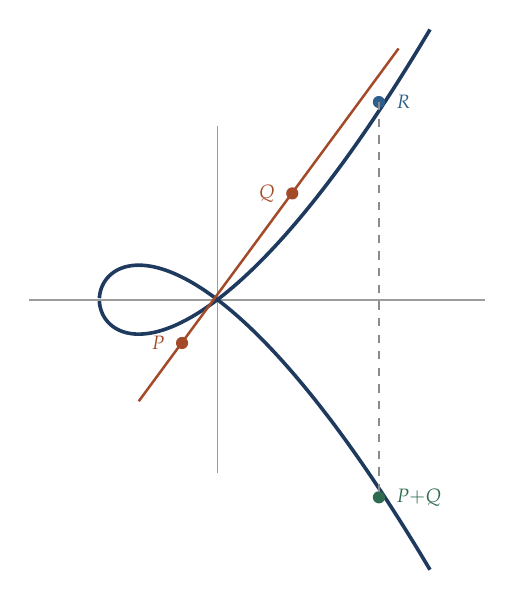
\begin{tikzpicture}[scale=1.0]
\draw[grau!60, line width=0.6pt] (-2.4,0) -- (3.4,0);
\draw[grau!60, line width=0.6pt] (0,-2.2) -- (0,2.2);
\draw[tief, line width=1.3pt, smooth, samples=60, domain=0.02:2.05]
  plot ({\x*\x-1.5}, {\x*(\x*\x-1.5)*0.62+1.1*\x*0.001});
\draw[tief, line width=1.3pt, smooth, samples=60, domain=0.02:2.05]
  plot ({\x*\x-1.5}, {-\x*(\x*\x-1.5)*0.62});
\coordinate (P) at (-0.45,-0.55);
\coordinate (Q) at (0.95,1.35);
\coordinate (R) at (2.55,3.55);
\fill[akzent] (P) circle (2.2pt); \fill[akzent] (0.95,1.35) circle (2.2pt);
\draw[akzent, line width=0.9pt] (-1.0,-1.29) -- (2.3,3.19);
\fill[mittel] (2.05,2.51) circle (2.2pt);
\fill[gruen] (2.05,-2.51) circle (2.2pt);
\draw[grau!70, line width=0.6pt, dashed] (2.05,2.51) -- (2.05,-2.51);
\node[font=\scriptsize, color=akzent, anchor=east] at (-0.55,-0.55) {$P$};
\node[font=\scriptsize, color=akzent, anchor=east] at (0.85,1.35) {$Q$};
\node[font=\scriptsize, color=mittel, anchor=west] at (2.15,2.51) {$R$};
\node[font=\scriptsize, color=gruen, anchor=west] at (2.15,-2.51) {$P{+}Q$};
\end{tikzpicture}
\end{center}

\schritt{Warum die Spiegelung}
Ohne sie wäre die Verknüpfung nicht assoziativ. Mit ihr gilt: Drei Punkte auf einer Geraden addieren sich zu $\mathcal{O}$.

\begin{center}
\begin{minipage}{0.88\textwidth}
\kursiv{Dass die so erklärte Verknüpfung tatsächlich eine Gruppe liefert, ist ein Satz --- und die Assoziativität ist der unangenehme Teil des Beweises. Elementar geführt ist er eine lange Rechnung; mit den Mitteln der algebraischen Geometrie ist er kurz. \textbf{Wir nehmen die Gruppeneigenschaft hier als gegeben} und prüfen sie an Beispielen nach.}
\end{minipage}
\end{center}

\schritt{Die Formeln}
Für $P=(x_1,y_1)$ und $Q=(x_2,y_2)$ mit $P \ne -Q$:
\[ \lambda = \begin{cases} \dfrac{y_2-y_1}{x_2-x_1} & \text{für } P \ne Q\\[10pt] \dfrac{3x_1^{2}+a}{2y_1} & \text{für } P = Q\end{cases} \]
\[ x_3 = \lambda^{2}-x_1-x_2, \qquad y_3 = \lambda\,(x_1-x_3)-y_1 \]

\begin{center}
\begin{minipage}{0.88\textwidth}
\kursiv{Die zweite Zeile für $\lambda$ ist die Ableitung der Kurve --- die Tangente. Sie ergibt sich durch implizites Differenzieren: $2y\,y' = 3x^2+a$. \textbf{Verdoppeln heißt, die Tangente zu legen}, und das ist die geometrische Entsprechung des Quadrierens aus Kapitel~12.}
\end{minipage}
\end{center}
\end{merksatz}

\section{Über endlichen Körpern}

\begin{merksatz}
\boxtitel{Dasselbe modulo einer Primzahl}
Die Formeln gelten unverändert, wenn man modulo $p$ rechnet. Die Division wird zur Multiplikation mit dem Inversen.

\schritt{Ein vollständiges Beispiel}
\[ E: \ y^{2} = x^{3}+2x+2 \quad\text{über}\quad \mathbb{F}_{17} \]

\kursiv{Ist $G=(5,1)$ ein Punkt?}
\[ 5^{3}+2\cdot5+2 = 125+10+2 = 137 = 8\cdot17+1 \ \to\ 1 \]
\[ y^{2} = 1 \quad \checkmark \]

\schritt{Verdoppeln}
\[ \lambda = \frac{3\cdot25+2}{2\cdot1} = \frac{77}{2} \]
\kursiv{Modulo 17:} $77 = 4\cdot17+9 \to 9$; $2^{-1} = 9$ wegen $2\cdot9 = 18 \equiv 1$.
\[ \lambda = 9\cdot9 = 81 = 4\cdot17+13 \ \to\ 13 \]
\[ x_3 = 13^{2}-5-5 = 169-10 = 159 = 9\cdot17+6 \ \to\ \mathbf{6} \]
\[ y_3 = 13\,(5-6)-1 = -14 \equiv \mathbf{3} \pmod{17} \]

\[ 2G = (6,3) \]

\kursiv{Probe:} $6^{3}+12+2 = 230 = 13\cdot17+9 \to 9$, und $3^{2} = 9$ \checkmark

\schritt{Die ganze Gruppe}
\begin{center}
{\small
\renewcommand{\arraystretch}{1.4}
\begin{tabular}{@{}P{1.0cm}P{1.6cm}P{1.0cm}P{1.6cm}P{1.0cm}P{1.6cm}@{}}
\toprule
$k$ & $kG$ & $k$ & $kG$ & $k$ & $kG$\\
\midrule
$1$ & $(5,1)$ & $8$ & $(13,7)$ & $15$ & $(3,16)$\\
$2$ & $(6,3)$ & $9$ & $(7,6)$ & $16$ & $(10,11)$\\
$3$ & $(10,6)$ & $10$ & $(7,11)$ & $17$ & $(6,14)$\\
$4$ & $(3,1)$ & $11$ & $(13,10)$ & $18$ & $(5,16)$\\
$5$ & $(9,16)$ & $12$ & $(0,11)$ & $19$ & $\mathcal{O}$\\
$6$ & $(16,13)$ & $13$ & $(16,4)$ & & \\
$7$ & $(0,6)$ & $14$ & $(9,1)$ & & \\
\bottomrule
\end{tabular}}
\end{center}

\begin{center}
\begin{minipage}{0.9\textwidth}
\textbf{Die Gruppe hat $19$ Elemente, und $G$ erzeugt sie alle.} $G$ ist also ein erzeugendes Element wie die Primitivwurzel in Kapitel~12.
\end{minipage}
\end{center}

\begin{center}
\begin{minipage}{0.88\textwidth}
\kursiv{Bemerkenswert ist die Symmetrie: $18G = (5,16)$ und $G = (5,1)$ --- und $1+16 = 17 \equiv 0$. Die Punkte $kG$ und $(19-k)G$ sind Spiegelbilder an der $x$-Achse, also entgegengesetzt. \textbf{Die Tabelle liest sich von beiden Enden.}}
\end{minipage}
\end{center}
\end{merksatz}

\begin{merksatz}
\boxtitel{Das Logarithmusproblem hier}
\begin{center}
\begin{minipage}{0.9\textwidth}
\textbf{Gegeben $G$ und $Q = kG$, bestimme $k$.}
\end{minipage}
\end{center}

\begin{center}
{\small
\renewcommand{\arraystretch}{1.5}
\begin{tabular}{@{}P{2.8cm}P{2.4cm}P{2.8cm}@{}}
\toprule
& \textbf{Restklassen} & \textbf{elliptisch}\\
\midrule
Durchprobieren & $n$ & $n$\\
Pollards Rho & $\sqrt n$ & $\sqrt n$\\
Indexrechnung & \textcolor{akzent}{$L_n[1/3]$} & \textcolor{gruen}{nicht bekannt}\\
\bottomrule
\end{tabular}}
\end{center}

\begin{center}
\begin{minipage}{0.9\textwidth}
\textbf{Die dritte Zeile ist der ganze Vorteil.} Bei elliptischen Kurven ist die Wurzelschranke nach heutigem Wissen das Beste --- also $2^{n/2}$ bei $n$ Bit.
\end{minipage}
\end{center}

\schritt{Die Folge für die Schlüssellängen}
\begin{center}
{\small
\renewcommand{\arraystretch}{1.48}
\begin{tabular}{@{}P{2.0cm}P{2.2cm}P{2.0cm}P{1.8cm}@{}}
\toprule
\textbf{Sicherheit} & \textbf{RSA/DH} & \textbf{elliptisch} & \textbf{Faktor}\\
\midrule
$112$ Bit & $2048$ & $224$ & $9{,}1$\\
$128$ Bit & $3072$ & $256$ & $12{,}0$\\
$192$ Bit & $7680$ & $384$ & $20{,}0$\\
$256$ Bit & $15\,360$ & $512$ & $30{,}0$\\
\bottomrule
\end{tabular}}
\end{center}

\begin{center}
\begin{minipage}{0.88\textwidth}
\kursiv{Der Grund für das Fehlen der Indexrechnung ist begrifflich: Sie sucht Elemente, die sich in kleine Faktoren zerlegen lassen. Auf einer elliptischen Kurve gibt es keinen Begriff von \enquote{klein} --- die Punkte tragen keine Größenordnung. \textbf{Ein Verfahren scheitert nicht an einer Schwierigkeit, sondern daran, dass sein zentraler Begriff fehlt.}}
\end{minipage}
\end{center}
\end{merksatz}

\section{Signaturen}

\begin{merksatz}
\boxtitel{Das Verfahren}
Öffentlich: die Kurve, $G$ und die Ordnung $n$. Der Unterzeichner hat $d$ geheim und $Q = dG$ öffentlich.

\begin{center}
{\small
\renewcommand{\arraystretch}{1.52}
\begin{tabular}{@{}P{2.0cm}P{6.6cm}@{}}
\toprule
\textbf{Signieren} & Wähle $k$ zufällig; setze $R = kG$ und $r = x_R \bmod n$.\\
& $s = k^{-1}\bigl(H(m)+r\,d\bigr) \bmod n$\\
& Die Signatur ist $(r,s)$.\\
\midrule
\textbf{Prüfen} & $u_1 = H(m)\,s^{-1}$, $u_2 = r\,s^{-1}$\\
& Prüfe $x\bigl(u_1G+u_2Q\bigr) \equiv r$\\
\bottomrule
\end{tabular}}
\end{center}

\schritt{Warum die Prüfung aufgeht}
\begin{align*}
u_1 G + u_2 Q &= H(m)s^{-1}G + r s^{-1} d G\\
&= s^{-1}\bigl(H(m)+rd\bigr)\,G\\
&= s^{-1}\cdot s\,k\,G && \text{(Definition von } s)\\
&= k\,G = R
\end{align*}
Also stimmt die $x$-Koordinate mit $r$ überein. \checkmark

\begin{center}
\begin{minipage}{0.88\textwidth}
\kursiv{Der Prüfer rechnet $R$ aus, ohne $k$ zu kennen --- er setzt es aus zwei bekannten Punkten zusammen. \textbf{Das ist der Kunstgriff des Verfahrens}, und er funktioniert, weil die Gruppenoperation kommutiert.}
\end{minipage}
\end{center}
\end{merksatz}

\begin{warnung}
\boxtitelr{Der Zufallswert darf sich nie wiederholen}
Werden zwei Nachrichten mit demselben $k$ signiert, so gilt
\[ s_1 = k^{-1}(h_1+rd), \qquad s_2 = k^{-1}(h_2+rd) \]

\schritt{Die Auflösung}
\[ s_1-s_2 = k^{-1}(h_1-h_2) \quad\Longrightarrow\quad k = \frac{h_1-h_2}{s_1-s_2} \]

Und daraus:
\[ d = \frac{s_1 k - h_1}{r} \]

\begin{center}
\begin{minipage}{0.9\textwidth}
\textbf{Zwei Signaturen mit demselben Zufallswert geben den geheimen Schlüssel vollständig preis.}
\end{minipage}
\end{center}

\begin{center}
\begin{minipage}{0.88\textwidth}
\kursiv{Man beachte, dass $r$ in beiden Fällen gleich ist --- das verrät die Wiederholung sogar öffentlich. \textbf{Der Angreifer braucht nur zwei Signaturen mit gleichem $r$ zu suchen}, und dann zwei Divisionen. Das ist derselbe Fehler wie beim Einmalschlüssel in Kapitel~9 und beim Zähler in Kapitel~10 --- zum dritten Mal in diesem Band, in neuer Gestalt.}
\end{minipage}
\end{center}

\schritt{Was tatsächlich geschah}
2010 wurde der Signaturschlüssel einer verbreiteten Spielkonsole veröffentlicht. Der Hersteller hatte einen festen Wert statt eines zufälligen verwendet.

\begin{center}
\begin{minipage}{0.88\textwidth}
\kursiv{Es war kein Fehler in der Mathematik, kein zu kurzer Schlüssel und keine Schwäche der Kurve --- eine Zeile Programmcode. Die Folge war, dass beliebige Software als vom Hersteller signiert ausgegeben werden konnte. \textbf{Der geheime Schlüssel ließ sich aus zwei öffentlich verfügbaren Signaturen berechnen.}}
\end{minipage}
\end{center}

\schritt{Die Abhilfe}
Man leitet $k$ aus dem geheimen Schlüssel und der Nachricht ab, statt es zu würfeln:
\[ k = \mathrm{HMAC}_{d}(H(m)) \]

\begin{center}
\begin{minipage}{0.88\textwidth}
\kursiv{Damit ist $k$ für jede Nachricht verschieden und für den Angreifer unvorhersehbar --- und das Verfahren kommt ohne Zufallsgenerator aus. \textbf{Man ersetzt eine Anforderung an die Umgebung durch eine Rechnung}, und das ist fast immer der sicherere Weg.}
\end{minipage}
\end{center}
\end{warnung}

\section{Der Bruchfall}

\begin{warnung}
\boxtitelr{Die Kurve muss stimmen}
\begin{center}
{\small
\renewcommand{\arraystretch}{1.52}
\begin{tabular}{@{}P{2.4cm}P{6.2cm}@{}}
\toprule
\textbf{Schwache Kurven} & Bei bestimmten Kurven lässt sich das Problem auf ein leichteres zurückführen und in polynomialer Zeit lösen.\\
\textbf{Kleine Ordnung} & Hat die Gruppe kleine Faktoren, so zerfällt das Problem in Teilprobleme.\\
\textbf{Punkte prüfen} & Liegt ein empfangener Punkt gar nicht auf der Kurve, so kann die Rechnung den Schlüssel verraten.\\
\bottomrule
\end{tabular}}
\end{center}

\schritt{Zur dritten Zeile}
Die Additionsformeln benutzen den Parameter $b$ nicht.

\begin{center}
\begin{minipage}{0.9\textwidth}
\textbf{Ein Angreifer kann daher einen Punkt einer \kursiv{anderen} Kurve senden, deren Gruppe kleine Ordnung hat --- und aus der Antwort den Schlüssel modulo dieser Ordnung erschließen.}
\end{minipage}
\end{center}

\begin{center}
\begin{minipage}{0.88\textwidth}
\kursiv{Nach genügend vielen solchen Anfragen setzt man den Schlüssel über den chinesischen Restsatz zusammen. Die Abhilfe ist eine Zeile: \textbf{Jeden empfangenen Punkt darauf prüfen, ob er die Kurvengleichung erfüllt.} Dass diese Zeile fehlte, hat wiederholt zu Angriffen geführt.}
\end{minipage}
\end{center}

\schritt{Und die Vertrauensfrage}
Die gebräuchlichen Kurven wurden von Normungsgremien festgelegt, teils mit Parametern unklarer Herkunft.

\begin{center}
\begin{minipage}{0.88\textwidth}
\kursiv{Nach den Enthüllungen von 2013 über einen manipulierten Zufallsgenerator wuchs das Misstrauen. Die Antwort waren Kurven mit \Begriff{nachvollziehbar zufälligen} Parametern --- jede Konstante wird aus einer öffentlichen Rechenvorschrift abgeleitet, so dass kein Spielraum für eine versteckte Hintertür bleibt. \textbf{Man ersetzt Vertrauen durch Nachprüfbarkeit}, und das ist dieselbe Denkweise wie beim offenen Wettbewerb aus Kapitel~10.}
\end{minipage}
\end{center}
\end{warnung}

\section{Übungsaufgaben}

\begin{aufgabe}
\boxtitel{Aufgabe 14.1 --- Punkte addieren}
Auf $E: y^{2} = x^{3}+2x+2$ über $\mathbb{F}_{17}$ mit $P = (5,1)$ und $Q = (6,3)$: Bestimmen Sie $P+Q$.

\loesung
\schritt{Schritt 1 --- Die Steigung}
\[ \lambda = \frac{3-1}{6-5} = \frac{2}{1} = 2 \]

\schritt{Schritt 2 --- Die neue $x$-Koordinate}
\[ x_3 = \lambda^{2}-x_1-x_2 = 4-5-6 = -7 \equiv 10 \pmod{17} \]

\schritt{Schritt 3 --- Die neue $y$-Koordinate}
\[ y_3 = \lambda\,(x_1-x_3)-y_1 = 2\,(5-10)-1 = -11 \equiv 6 \pmod{17} \]

\[ P+Q = (10,\ 6) \]

\schritt{Schritt 4 --- Die Probe}
\kursiv{Liegt der Punkt auf der Kurve?}
\[ 10^{3}+2\cdot10+2 = 1000+22 = 1022 \]
\[ 1022 = 60\cdot17+2 \ \to\ 2 \]
\[ 6^{2} = 36 = 2\cdot17+2 \ \to\ 2 \quad \checkmark \]

\schritt{Schritt 5 --- Die zweite Probe}
Nach der Tabelle in Abschnitt 14.3 ist $P = G$, $Q = 2G$ und $3G = (10,6)$.
\[ G + 2G = 3G \quad \checkmark \]

\schritt{Schritt 6 --- Ein Sonderfall}
Was ist $P + (5,16)$?

Wegen $1+16 = 17 \equiv 0$ sind die beiden Punkte entgegengesetzt:
\[ (5,1) + (5,16) = \mathcal{O} \]

\begin{center}
\begin{minipage}{0.88\textwidth}
\kursiv{Die Formel versagt hier --- der Nenner $x_2-x_1$ wäre null. \textbf{Das ist kein Mangel, sondern der Fernpunkt}: Die Gerade durch zwei senkrecht übereinanderliegende Punkte ist senkrecht und schneidet die Kurve kein drittes Mal im Endlichen. Jede Umsetzung muss diesen Fall gesondert behandeln, und das ist eine bekannte Fehlerquelle.}
\end{minipage}
\end{center}
\end{aufgabe}

\begin{aufgabe}
\boxtitel{Aufgabe 14.2 --- Schlüsseltausch auf der Kurve}
Alice wählt $a = 3$, Bob $b = 10$. Führen Sie den Tausch mit derselben Kurve durch.

\loesung
\schritt{Schritt 1 --- Die öffentlichen Punkte}
Aus der Tabelle:
\[ A = 3G = (10,6), \qquad B = 10G = (7,11) \]

\schritt{Schritt 2 --- Alice rechnet}
\[ 10\cdot A = 10\cdot(3G) = 30\,G \]

Wegen $\mathcal{O} = 19G$ gilt $30G = 11G$:
\[ 30 = 19+11 \quad\Longrightarrow\quad 30G = 11G = (13,10) \]

\schritt{Schritt 3 --- Bob rechnet}
\[ 3\cdot B = 3\cdot(10G) = 30\,G = (13,10) \quad \checkmark \]

\begin{center}
\begin{minipage}{0.9\textwidth}
\textbf{Beide erhalten $(13,10)$.} Der gemeinsame Schlüssel wird üblicherweise aus der $x$-Koordinate abgeleitet.
\end{minipage}
\end{center}

\schritt{Schritt 4 --- Was der Mitleser sieht}
Er kennt die Kurve, $G$, $A = (10,6)$ und $B = (7,11)$.

Um $a$ zu finden, müsste er die Tabelle durchgehen --- bei $19$ Punkten in Sekunden.

\begin{center}
\begin{minipage}{0.88\textwidth}
\kursiv{Praktisch verwendete Kurven haben Gruppenordnungen um $2^{256}$. \textbf{Auch hier gilt: Das Beispiel zeigt die Rechnung, nicht die Sicherheit.}}
\end{minipage}
\end{center}

\schritt{Schritt 5 --- Der Vergleich mit Kapitel 12}
\begin{center}
{\small
\renewcommand{\arraystretch}{1.48}
\begin{tabular}{@{}P{2.4cm}P{2.4cm}P{2.6cm}@{}}
\toprule
& \textbf{Kapitel 12} & \textbf{hier}\\
\midrule
Menge & Reste mod $p$ & Kurvenpunkte\\
Verknüpfung & Multiplikation & Punktaddition\\
Potenzieren & $g^{a}$ & $aG$\\
Schwer & Logarithmus & Logarithmus\\
\bottomrule
\end{tabular}}
\end{center}

\begin{center}
\begin{minipage}{0.88\textwidth}
\kursiv{Die Verfahren sind identisch; nur die Gruppe ist ausgetauscht. \textbf{Das ist der Ertrag der abstrakten Formulierung}: Wer Diffie-Hellman für Gruppen versteht, versteht es für jede Gruppe --- und kann die beste wählen.}
\end{minipage}
\end{center}
\end{aufgabe}

\begin{aufgabe}
\boxtitel{Aufgabe 14.3 --- Den Schlüssel aus zwei Signaturen}
Ein Unterzeichner hat mit demselben $k$ zwei Nachrichten signiert. Bekannt sind $n$, $r$, $s_1$, $s_2$, $h_1$, $h_2$. Bestimmen Sie den geheimen Schlüssel.

\loesung
\schritt{Schritt 1 --- Die beiden Gleichungen}
\[ s_1 = k^{-1}(h_1+r\,d), \qquad s_2 = k^{-1}(h_2+r\,d) \]

\schritt{Schritt 2 --- Subtrahieren}
\[ s_1-s_2 = k^{-1}\bigl[(h_1+rd)-(h_2+rd)\bigr] = k^{-1}(h_1-h_2) \]

\begin{center}
\begin{minipage}{0.9\textwidth}
\textbf{Der Term mit $d$ fällt heraus.}
\end{minipage}
\end{center}

\schritt{Schritt 3 --- $k$ bestimmen}
\[ k = \frac{h_1-h_2}{s_1-s_2} \bmod n \]

\schritt{Schritt 4 --- $d$ bestimmen}
Aus $s_1 k = h_1 + r d$:
\[ d = \frac{s_1 k - h_1}{r} \bmod n \]

\schritt{Schritt 5 --- Ein Zahlenbeispiel}
Mit $n = 19$, $r = 13$, $h_1 = 5$, $h_2 = 9$, $s_1 = 7$, $s_2 = 3$:
\[ k = \frac{5-9}{7-3} = \frac{-4}{4} = -1 \equiv 18 \pmod{19} \]

\[ d = \frac{7\cdot18-5}{13} = \frac{126-5}{13} = \frac{121}{13} \bmod 19 \]

\kursiv{Zähler:} $121 = 6\cdot19+7 \to 7$.\\
\kursiv{Inverses von $13$:} $13\cdot3 = 39 = 2\cdot19+1$, also $13^{-1} = 3$.
\[ d = 7\cdot3 = 21 \equiv \mathbf{2} \pmod{19} \]

\schritt{Schritt 6 --- Die Probe}
\[ s_1 = k^{-1}(h_1+rd) = 18^{-1}\,(5+13\cdot2) = 18^{-1}\cdot31 \]
\kursiv{$31 \equiv 12$; $18 \equiv -1$, also $18^{-1} = 18$.}
\[ s_1 = 18\cdot12 = 216 = 11\cdot19+7 \ \to\ \mathbf{7} \quad \checkmark \]

\schritt{Schritt 7 --- Der Aufwand}
\begin{center}
\begin{minipage}{0.9\textwidth}
\textbf{Zwei Subtraktionen, zwei Divisionen.} Der Angreifer braucht keine Rechenkraft, nur zwei Signaturen mit gleichem $r$.
\end{minipage}
\end{center}

\begin{center}
\begin{minipage}{0.88\textwidth}
\kursiv{Und $r$ steht offen in der Signatur --- er muss also nur nach Wiederholungen suchen. Bei einem festen $k$ ist $r$ in \kursiv{allen} Signaturen gleich, und der Angriff gelingt beim ersten Paar. \textbf{Ein Verfahren, dessen Sicherheit an einem einzigen Zufallswert hängt, bricht vollständig, wenn dieser Wert versagt} --- und das unterscheidet die Signatur von der Verschlüsselung, wo eine Wiederholung nur die betroffenen Nachrichten gefährdet.}
\end{minipage}
\end{center}

\schritt{Schritt 8 --- Sogar Teilinformation genügt}
Kennt der Angreifer auch nur wenige Bit von $k$ --- etwa weil der Zufallsgenerator leicht verzerrt ist --- so lässt sich $d$ aus vielen Signaturen mit Gitterverfahren gewinnen.

\begin{center}
\begin{minipage}{0.86\textwidth}
\kursiv{Einige hundert Signaturen mit je vier bekannten Bit genügen. Das ist praktisch bedeutsam, weil Seitenkanäle aus Kapitel~10 genau solche Teilinformation liefern. \textbf{Ein fast perfekter Zufallsgenerator ist hier nicht fast sicher, sondern unsicher.}}
\end{minipage}
\end{center}
\end{aufgabe}

\begin{geschichte}
\boxtitelg{Zwei Vorschläge im selben Jahr}
\Person{Neal Koblitz} an der Universität Washington und \Person{Victor Miller} bei IBM schlugen 1985 unabhängig voneinander vor, elliptische Kurven für die Kryptographie zu verwenden.

\begin{center}
\begin{minipage}{0.9\textwidth}
\kursiv{Beide kannten die Kurven aus der Zahlentheorie, wo sie seit dem 19.\ Jahrhundert untersucht werden --- unter anderem im Zusammenhang mit der Fermatschen Vermutung, deren Beweis 1995 wesentlich auf ihnen beruht. \textbf{Ein Gegenstand reiner Grundlagenforschung wurde zur Grundlage der digitalen Sicherheit}, und zwar ohne dass jemand es geplant hätte.}
\end{minipage}
\end{center}

\schritt{Die lange Anlaufzeit}
Die Verfahren brauchten fünfzehn Jahre bis zur breiten Anwendung.

\begin{center}
\begin{minipage}{0.9\textwidth}
\kursiv{Gründe waren Patentfragen, die höhere Komplexität der Umsetzung und ein grundsätzliches Misstrauen: Die zugrundeliegende Mathematik galt als schwerer überprüfbar. Erst als die Schlüssellängen für RSA unbequem wurden --- insbesondere bei Mobilgeräten --- setzte sich der Wechsel durch.}
\end{minipage}
\end{center}

\schritt{Die Kurve mit dem Zweifel}
2013 wurde bekannt, dass ein genormter Zufallsgenerator auf elliptischen Kurven vermutlich eine Hintertür enthielt.

\begin{center}
\begin{minipage}{0.9\textwidth}
\kursiv{Der Verdacht bestand seit 2007 --- zwei Forscher hatten gezeigt, dass die Kenntnis eines bestimmten Zusammenhangs zwischen zwei Konstanten die Vorhersage aller Ausgaben erlaubt. Die Konstanten waren ohne Begründung festgelegt worden. \textbf{Der Generator wurde 2014 zurückgezogen}; die Kurven selbst waren nie betroffen, aber das Vertrauen war beschädigt.}
\end{minipage}
\end{center}

\schritt{Die Antwort}
\Person{Daniel Bernstein} und andere entwarfen ab 2005 Kurven, deren Parameter sich vollständig aus nachvollziehbaren Regeln ergeben.

\begin{center}
\begin{minipage}{0.9\textwidth}
\kursiv{Jede Konstante wird begründet --- etwa als kleinste Zahl mit einer bestimmten Eigenschaft. Zusätzlich wurden die Formeln so gewählt, dass Sonderfälle wie in Aufgabe 14.1 nicht auftreten und die Rechnung stets gleich lange dauert. \textbf{Der Entwurf schließt die Fehler aus, statt vor ihnen zu warnen} --- und das ist die eigentliche Lehre der letzten beiden Kapitel.}
\end{minipage}
\end{center}
\end{geschichte}

\begin{forschung}
\boxtitelp{Elliptische Kurven heute}
\begin{center}
{\small
\renewcommand{\arraystretch}{1.45}
\begin{tabular}{@{}P{2.8cm}P{5.4cm}@{}}
\toprule
\textbf{Verbreitung} & Bei neuen Anwendungen der Regelfall; in Mobilfunk, Messengern und Kartenzahlung.\\
\textbf{Paarungen} & Besondere Kurven erlauben eine Verknüpfung zweier Punkte zu einem Körperelement --- Grundlage für Verfahren, die anders nicht möglich wären.\\
\textbf{Isogenien} & Abbildungen zwischen Kurven; galten als quantensicherer Kandidat.\\
\bottomrule
\end{tabular}}
\end{center}

\schritt{Zur zweiten Zeile}
Eine Paarung ist eine Abbildung mit
\[ e(aP,\,bQ) = e(P,Q)^{ab} . \]

\begin{center}
\begin{minipage}{0.88\textwidth}
\kursiv{Damit lassen sich Dinge bauen, die sonst unerreichbar sind: Schlüsseltausch zu dritt in einer Runde, Verschlüsselung an eine Kennung statt an einen Schlüssel, und kurze Beweise für umfangreiche Behauptungen. \textbf{Die Paarung war zunächst als Angriffswerkzeug entdeckt worden} --- sie führt das Problem auf eines in einem Körper zurück und schwächt bestimmte Kurven. Erst später erkannte man sie als Baustein.}
\end{minipage}
\end{center}

\schritt{Zur dritten Zeile}
Ein auf Isogenien beruhendes Verfahren galt lange als aussichtsreicher Kandidat für die Zeit nach dem Quantenrechner.

\begin{center}
\begin{minipage}{0.88\textwidth}
\kursiv{2022 wurde es gebrochen --- klassisch, auf einem einzelnen Rechner, binnen Stunden. Der Angriff beruhte auf einem Satz von 1997, den niemand in diesem Zusammenhang gesehen hatte. \textbf{Ein Verfahren, das fünf Jahre lang geprüft worden war, fiel an einem Nachmittag}, und das ist die beste Mahnung zur Vorsicht bei neuen Annahmen. Kapitel~15 behandelt die verbliebenen Kandidaten.}
\end{minipage}
\end{center}
\end{forschung}

\begin{merksatz}
\boxtitel{Was Sie jetzt können}
\begin{center}
\renewcommand{\arraystretch}{1.5}
\begin{tabular}{@{}P{3.0cm}P{5.6cm}@{}}
\toprule
\textbf{Definition 14.1} & Kurve, Fernpunkt, Gruppengesetz\\
\textbf{Die Formeln} & Sehne und Tangente, modular gerechnet\\
\textbf{Der Vorteil} & keine Indexrechnung, Faktor $12$\\
\textbf{Signaturen} & der Prüfer setzt $R$ zusammen\\
\textbf{Der Bruchfall} & $k$ zweimal heißt Schlüssel verloren\\
\bottomrule
\end{tabular}
\end{center}

\begin{center}
\begin{minipage}{0.88\textwidth}
\kursiv{Damit endet Teil~V. Alle Verfahren dieses Teils --- Diffie-Hellman, RSA, elliptische Kurven --- fallen durch dasselbe Quantenverfahren. Das letzte Kapitel fragt, was danach kommt.}
\end{minipage}
\end{center}
\end{merksatz}

\part{Aktueller Stand}

\chapter{Was Information leistet}

\section{Die Bedrohung}

\begin{merksatz}
\boxtitel{Zwei Quantenverfahren, zwei Wirkungen}
\begin{center}
{\small
\renewcommand{\arraystretch}{1.55}
\begin{tabular}{@{}P{2.0cm}P{3.0cm}P{3.4cm}@{}}
\toprule
& \textbf{Shor, 1994} & \textbf{Grover, 1996}\\
\midrule
Leistet & Faktorisieren und diskrete Logarithmen in polynomialer Zeit & Durchsuchen in $\sqrt N$ statt $N$\\
Betrifft & \textcolor{akzent}{Teil V vollständig} & Teil IV teilweise\\
Abhilfe & \textcolor{akzent}{keine} & \textcolor{gruen}{Länge verdoppeln}\\
\bottomrule
\end{tabular}}
\end{center}

\schritt{Die Bilanz je Baustein}
\begin{center}
{\small
\renewcommand{\arraystretch}{1.48}
\begin{tabular}{@{}P{2.6cm}P{2.0cm}P{2.6cm}@{}}
\toprule
\textbf{Baustein} & \textbf{klassisch} & \textbf{mit Quantenrechner}\\
\midrule
AES-128 & $128$ & $64$ Bit\\
AES-256 & $256$ & \textcolor{gruen}{$128$ Bit}\\
SHA-256 & $128$ & $\approx 85$ Bit\\
SHA-512 & $256$ & \textcolor{gruen}{$\approx 170$ Bit}\\
RSA-3072 & $138$ & \textcolor{akzent}{gebrochen}\\
Elliptisch-$256$ & $128$ & \textcolor{akzent}{gebrochen}\\
\bottomrule
\end{tabular}}
\end{center}

\begin{center}
\begin{minipage}{0.9\textwidth}
\textbf{Die ersten vier Zeilen sind ein Umstellungsaufwand. Die letzten beiden sind ein Bruch.}
\end{minipage}
\end{center}

\begin{center}
\begin{minipage}{0.88\textwidth}
\kursiv{Der Unterschied ist grundsätzlich: Grover halbiert den Exponenten --- man verdoppelt die Schlüssellänge und ist wieder da, wo man war. Shor macht das Problem polynomial --- \textbf{längere Schlüssel helfen nicht}, weil der Aufwand nur polynomial mitwächst.}
\end{minipage}
\end{center}
\end{merksatz}

\begin{warnung}
\boxtitelr{Warum die Umstellung heute nötig ist}
\begin{center}
\begin{minipage}{0.9\textwidth}
\textbf{Wer heute aufgezeichneten Verkehr speichert, kann ihn entschlüsseln, sobald ein Quantenrechner verfügbar ist.}
\end{minipage}
\end{center}

\schritt{Die Rechnung}
\begin{center}
{\small
\renewcommand{\arraystretch}{1.5}
\begin{tabular}{@{}P{3.4cm}P{1.6cm}P{2.6cm}@{}}
\toprule
\textbf{Größe} & \textbf{Jahre} & \\
\midrule
Geheimhaltungs\-dauer & $30$ & Patientendaten\\
Umstellungsdauer & $10$ & Infrastruktur\\
\midrule
Summe & $\mathbf{40}$ & \\
\bottomrule
\end{tabular}}
\end{center}

\begin{center}
\begin{minipage}{0.88\textwidth}
\kursiv{Ist ein Quantenrechner in weniger als vierzig Jahren verfügbar, so ist heute verschlüsselter Verkehr betroffen. \textbf{Niemand kann den Zeitpunkt zuverlässig nennen} --- und genau deshalb ist die Umstellung keine Frage der Vorhersage, sondern der Vorsicht. Für Patientendaten mit lebenslanger Schutzdauer verschärft sich die Rechnung erheblich.}
\end{minipage}
\end{center}

\schritt{Der Stand der Technik}
Gegenwärtig arbeiten Quantenrechner mit einigen hundert bis wenigen tausend physikalischen Quantenbits.

\begin{center}
\begin{minipage}{0.88\textwidth}
\kursiv{Für einen $2048$-Bit-Schlüssel bräuchte man nach heutigen Schätzungen einige Millionen \kursiv{fehlerkorrigierte} Quantenbits --- und ein fehlerkorrigiertes erfordert tausend oder mehr physikalische. Der Abstand beträgt also mehrere Größenordnungen. \textbf{Er schrumpft, und die Schrumpfungsrate ist unbekannt.}}
\end{minipage}
\end{center}
\end{warnung}

\section{Was an die Stelle tritt}

\begin{merksatz}
\boxtitel{Vier Familien}
\begin{center}
{\small
\renewcommand{\arraystretch}{1.52}
\begin{tabular}{@{}P{2.2cm}P{3.0cm}P{3.2cm}@{}}
\toprule
\textbf{Familie} & \textbf{beruht auf} & \textbf{Stand}\\
\midrule
Gitter & kürzeste Vektoren in hochdimensionalen Gittern & \textcolor{gruen}{genormt}\\
Codes & Decodieren zufälliger linearer Codes & \textcolor{gruen}{genormt}\\
Hashwerte & nur Kapitel 11 & \textcolor{gruen}{genormt, langsam}\\
Mehrere Variablen & Gleichungssysteme über endlichen Körpern & \textcolor{mittel}{teils gebrochen}\\
\bottomrule
\end{tabular}}
\end{center}

\schritt{Die zweite Zeile ist bemerkenswert}
Das Decodierproblem zufälliger linearer Codes ist genau das Problem aus Kapitel~6 --- nur ohne die Struktur, die Codes brauchbar macht.

\begin{center}
\begin{minipage}{0.88\textwidth}
\kursiv{\Person{Robert McEliece} schlug 1978 ein darauf beruhendes Verfahren vor, zwei Jahre nach Diffie und Hellman. \textbf{Es ist seit fast fünfzig Jahren ungebrochen} --- länger als jedes andere Verfahren mit öffentlichem Schlüssel. Durchgesetzt hat es sich nie, weil der öffentliche Schlüssel etwa ein Megabyte umfasst.}
\end{minipage}
\end{center}

\schritt{Die dritte Zeile}
Signaturen lassen sich allein aus Hashfunktionen bauen --- ohne jede zahlentheoretische Annahme.

\begin{center}
\begin{minipage}{0.88\textwidth}
\kursiv{Das ist die konservativste Wahl: Sie setzt nur voraus, dass die Hashfunktion hält, und nach Kapitel~11 ist das die am wenigsten bedrohte Annahme. Der Preis sind lange Signaturen und teils begrenzte Nutzungszahlen. \textbf{Für Aufgaben wie das Signieren von Aktualisierungen, die selten und langfristig erfolgen, ist das die richtige Abwägung.}}
\end{minipage}
\end{center}
\end{merksatz}

\begin{warnung}
\boxtitelr{Die Annahmen sind jung}
\begin{center}
{\small
\renewcommand{\arraystretch}{1.48}
\begin{tabular}{@{}P{2.6cm}P{2.2cm}P{2.8cm}@{}}
\toprule
\textbf{Annahme} & \textbf{geprüft seit} & \\
\midrule
Faktorisierung & $\approx 2300$ Jahren & Euklid\\
Diskreter Logarithmus & $50$ Jahren & \\
Gitterprobleme & $\approx 30$ Jahren & \\
Isogenien & $15$ Jahren & \textcolor{akzent}{gebrochen 2022}\\
\bottomrule
\end{tabular}}
\end{center}

\begin{center}
\begin{minipage}{0.9\textwidth}
\textbf{Die neuen Verfahren beruhen auf Problemen, die erheblich weniger lange geprüft sind als die alten.}
\end{minipage}
\end{center}

\begin{center}
\begin{minipage}{0.88\textwidth}
\kursiv{Der Fall von 2022 ist die Mahnung: Ein Verfahren, das fünf Jahre im Normungsverfahren geprüft worden war, fiel binnen Stunden auf einem gewöhnlichen Rechner --- durch einen Satz von 1997. \textbf{Die Prüfdauer ist die einzige verfügbare Evidenz, und sie ist bei den neuen Verfahren kurz.}}
\end{minipage}
\end{center}

\schritt{Die Antwort der Praxis}
Man kombiniert: klassischer und neuer Schlüsseltausch zugleich, der Sitzungsschlüssel aus beiden abgeleitet.

\begin{center}
\begin{minipage}{0.88\textwidth}
\kursiv{Das hält, solange \kursiv{eines} von beiden hält --- gegen einen Quantenrechner das neue, gegen einen Fehler im neuen das alte. \textbf{Es ist die Kombinationstherapie aus Band 18, Kapitel~14}, mit derselben Voraussetzung: Die Verfahren müssen unabhängig sein.}
\end{minipage}
\end{center}
\end{warnung}

\section{Vier Muster}

\begin{merksatz}
\boxtitel{Muster 1 --- eine Ungleichung, immer wieder}
\begin{center}
{\small
\renewcommand{\arraystretch}{1.48}
\begin{tabular}{@{}P{1.8cm}P{6.6cm}@{}}
\toprule
$2$ & $\Ent \le \lb n$ --- das Maximum bei Gleichverteilung.\\
$3$ & $L \ge \Ent$ --- keine Codierung unterbietet die Entropie.\\
$4$ & $D(p\|q) \ge 0$ --- und $I(X;Y)\ge0$ als Sonderfall.\\
$8$ & Die Fisher-Information als Krümmung von $D$.\\
\bottomrule
\end{tabular}}
\end{center}

\begin{center}
\begin{minipage}{0.9\textwidth}
\textbf{Viermal derselbe Beweis: Jensen auf den Logarithmus, mit einer geschickt gewählten Konstante in der Summe.}
\end{minipage}
\end{center}

\begin{center}
\begin{minipage}{0.88\textwidth}
\kursiv{Alle sind Sonderfälle von $D(p\|q)\ge0$. \textbf{Die relative Entropie ist das eine Werkzeug, auf dem die gesamte Informationstheorie ruht} --- und sie taucht in Kapitel~8 als statistischer Begriff wieder auf, ohne dass sie sich verändert hätte.}
\end{minipage}
\end{center}
\end{merksatz}

\begin{merksatz}
\boxtitel{Muster 2 --- das Typische trägt alles}
\begin{center}
{\small
\renewcommand{\arraystretch}{1.48}
\begin{tabular}{@{}P{1.8cm}P{6.6cm}@{}}
\toprule
$3$ & Man codiert nur die typischen Folgen und lässt den Rest scheitern.\\
$5$ & $2^{n\Ent}$ von $2^{n}$ Folgen tragen die ganze Wahrscheinlichkeit.\\
$6$ & Gute Codes korrigieren nur die typischen Fehler, nicht alle.\\
$7$ & Fast alle Folgen sind inkomprimierbar --- und kommen nie vor.\\
\bottomrule
\end{tabular}}
\end{center}

\begin{center}
\begin{minipage}{0.9\textwidth}
\textbf{Die Informationstheorie handelt nicht vom Möglichen, sondern vom Wahrscheinlichen.}
\end{minipage}
\end{center}

\begin{center}
\begin{minipage}{0.88\textwidth}
\kursiv{Darin liegt ihr Unterschied zur Kombinatorik und zur Codierungstheorie klassischer Prägung. Shannons Beweis in Kapitel~5 verzichtet auf die Garantie für alle Fälle und gewinnt dadurch die Kapazität. \textbf{Wer alles korrigieren will, erreicht weniger als wer das Typische korrigiert} --- das ist eine der überraschendsten Einsichten dieses Bandes.}
\end{minipage}
\end{center}
\end{merksatz}

\begin{merksatz}
\boxtitel{Muster 3 --- derselbe Fehler, dreimal}
\begin{center}
{\small
\renewcommand{\arraystretch}{1.48}
\begin{tabular}{@{}P{1.8cm}P{6.6cm}@{}}
\toprule
$9$ & Einmalschlüssel zweimal benutzt: $C_1\oplus C_2 = M_1\oplus M_2$.\\
$10$ & Zählerwert zweimal benutzt: derselbe Schlüsselstrom.\\
$14$ & Zufallswert zweimal benutzt: der geheime Schlüssel fällt.\\
\bottomrule
\end{tabular}}
\end{center}

\begin{center}
\begin{minipage}{0.9\textwidth}
\textbf{Dreimal dieselbe Ursache, dreimal ein anderes Verfahren, dreimal ein vollständiger Bruch.}
\end{minipage}
\end{center}

\begin{center}
\begin{minipage}{0.88\textwidth}
\kursiv{Bei Venona war es doppelt gedrucktes Papier, bei den Betriebsarten ein Neustart, bei der Spielkonsole eine Zeile Programmcode. \textbf{Die Mathematik war in allen drei Fällen einwandfrei.} Das ist der durchgehende Befund von Teil~IV und V: Verfahren fallen nicht durch Kryptanalyse, sondern durch Umsetzung.}
\end{minipage}
\end{center}
\end{merksatz}

\begin{merksatz}
\boxtitel{Muster 4 --- Schranken sind einseitig}
\begin{center}
{\small
\renewcommand{\arraystretch}{1.48}
\begin{tabular}{@{}P{1.8cm}P{6.6cm}@{}}
\toprule
$1$ & Die Wägeschranke schließt aus; sie garantiert nicht.\\
$6$ & Die Kugelpackungsschranke verbietet Codes; sie liefert keine.\\
$7$ & $K$ lässt sich von oben abschätzen, nie von unten.\\
$11$ & Die Geburtstagsschranke ist eine obere Grenze für die Sicherheit.\\
\bottomrule
\end{tabular}}
\end{center}

\begin{center}
\begin{minipage}{0.9\textwidth}
\textbf{Fast alle Schranken dieses Bandes sagen, was nicht geht.} Dass etwas geht, ist stets ein eigener Satz --- und oft der schwierigere.
\end{minipage}
\end{center}

\begin{center}
\begin{minipage}{0.88\textwidth}
\kursiv{Shannons Kanalcodierungstheorem ist das klarste Beispiel: Die Umkehrung folgt aus zwei Ungleichungen, die Erreichbarkeit brauchte einen nicht konstruktiven Beweis und sechzig Jahre bis zur Umsetzung. \textbf{Bei MD5 lag zwischen Schranke und Wirklichkeit der Faktor $10^{14}$} --- in die ungünstige Richtung.}
\end{minipage}
\end{center}
\end{merksatz}

\section{Was nicht die Mathematik ist}

\begin{warnung}
\boxtitelr{Die Bilanz der drei Warnungen}
\begin{center}
{\small
\renewcommand{\arraystretch}{1.5}
\begin{tabular}{@{}P{2.4cm}P{6.2cm}@{}}
\toprule
\textbf{Erste} & Information ist nicht Bedeutung. Bestätigt in Kapitel~1 und 7: Eine zufällige Folge hat maximale Information und minimalen Gehalt.\\
\textbf{Zweite} & Sätze gelten für Grenzwerte. Bestätigt in Kapitel~5: Die Kapazität ist erreichbar --- bei Blocklängen in den Tausenden.\\
\textbf{Dritte} & Sicherheit ist nicht beweisbar. Bestätigt in jedem Kapitel von Teil~IV und V.\\
\bottomrule
\end{tabular}}
\end{center}

\schritt{Zur dritten Warnung}
\begin{center}
\begin{minipage}{0.9\textwidth}
\textbf{Mit einer einzigen Ausnahme --- dem Einmalschlüssel --- beruht jedes Verfahren dieses Bandes auf einer unbewiesenen Annahme.}
\end{minipage}
\end{center}

\begin{center}
\begin{minipage}{0.88\textwidth}
\kursiv{Und die Ausnahme ist praktisch unbrauchbar, wie Satz 9.3 beweist. \textbf{Die Sicherheit der digitalen Welt ruht auf der Vermutung, dass bestimmte Rechenprobleme schwer sind} --- und ein Beweis dafür würde zugleich $\mathsf{P}\ne\mathsf{NP}$ zeigen, also eines der Millenniumsprobleme lösen.}
\end{minipage}
\end{center}

\schritt{Und die eigentliche Schwachstelle}
\begin{center}
{\small
\renewcommand{\arraystretch}{1.5}
\begin{tabular}{@{}P{2.4cm}P{6.2cm}@{}}
\toprule
\textbf{Selten} & Ein Verfahren wird durch Kryptanalyse gebrochen.\\
\textbf{Häufig} & Ein korrektes Verfahren wird falsch verwendet.\\
\textbf{Sehr häufig} & Der Angriff umgeht die Mathematik vollständig --- Seitenkanäle, Verkehrsdaten, Schlüsselverwaltung, Menschen.\\
\bottomrule
\end{tabular}}
\end{center}

\begin{center}
\begin{minipage}{0.88\textwidth}
\kursiv{Der Mann in der Mitte aus Kapitel~12 braucht keinerlei Rechenkraft. Der Fehlerangriff aus Kapitel~13 braucht einen Spannungsstoß. Der Zeitangriff aus Kapitel~11 braucht eine Stoppuhr. \textbf{Die Mathematik ist der am besten gesicherte Teil des Systems} --- und deshalb greift niemand sie an.}
\end{minipage}
\end{center}
\end{warnung}

\section{Sechs Sätze, die bleiben}

\begin{merksatz}
\boxtitel{Die Bilanz}
\begin{center}
{\small
\renewcommand{\arraystretch}{1.55}
\begin{tabular}{@{}P{0.7cm}P{7.7cm}@{}}
\toprule
$1$ & Der Informationsgehalt hängt allein von der Wahrscheinlichkeit ab --- drei schwache Forderungen legen ihn fest.\\
$2$ & Die Entropie ist die Grenze der Kompression, und sie ist erreichbar.\\
$3$ & Über einen gestörten Kanal lässt sich bis zur Kapazität beliebig zuverlässig übertragen. Darüber gar nicht.\\
$4$ & Fast alle Folgen sind unkomprimierbar, und man kann es keiner einzelnen nachweisen.\\
$5$ & Perfekte Geheimhaltung verlangt einen Schlüssel so lang wie die Nachricht.\\
$6$ & Alles andere beruht auf einer Annahme.\\
\bottomrule
\end{tabular}}
\end{center}
\end{merksatz}

\begin{merksatz}
\boxtitel{Ein Schlusswort}
\begin{center}
\begin{minipage}{0.9\textwidth}
Dieser Band begann mit der Behauptung, eine Nachricht habe ein Gewicht, das sich in Bit angeben lässt --- und dass dieses Gewicht nicht davon abhängt, was sie bedeutet.

Fünfzehn Kapitel später lässt sich sagen, was aus dieser Beschränkung geworden ist. Sie hat eine Theorie ermöglicht, die für jede Art von Nachricht gleichermaßen gilt: für Diagnoseschlüssel und Funksignale, für Erbgutsequenzen und Passwörter. Und sie hat Sätze hervorgebracht, die man ohne sie nicht einmal hätte formulieren können --- über Grenzen, die niemand unterbietet, und über Verfahren, die sie erreichen.

Der Preis war von Anfang an klar und ist es geblieben. Der Begriff sagt nichts darüber, ob eine Nachricht wahr ist, ob sie nützt oder ob sie verstanden wird. Er misst allein, wie sehr sie Ungewissheit auflöst --- und das ist eine Frage an den Empfänger, nicht an die Nachricht.
\end{minipage}
\end{center}

\begin{center}
\begin{minipage}{0.88\textwidth}
\kursiv{In der zweiten Hälfte kehrt sich das Vorzeichen um, und der Begriff bleibt derselbe. Geheimhaltung heißt, dass der Geheimtext die Ungewissheit des Mitlesers \kursiv{nicht} auflöst --- Definition 9.1 ist Kapitel~4 mit umgekehrtem Wunsch. \textbf{Dieselbe Größe misst, was ankommen soll, und was nicht ankommen darf.}}
\end{minipage}
\end{center}

\begin{center}
\begin{minipage}{0.88\textwidth}
\kursiv{Damit steht dieser Band neben den drei vorangegangenen. Die Statistik sagt, was die Daten hergeben. Die Biomathematik sagt, woran es liegt. Die Optimierung sagt, was es kostet. Und die Informationstheorie sagt, was überhaupt übertragbar ist --- \textbf{und sie sagt es in einer Einheit, die man nachrechnen kann.}}
\end{minipage}
\end{center}
\end{merksatz}

\appendix
\part{Anhang}

\newcommand{\lit}[3]{\vspace{5pt}\noindent\textbf{[#1]} #2\par\nopagebreak\vspace{1pt}{\small\itshape\color{grau} #3}\par\vspace{2pt}}

\chapter{Formelsammlung und Übersicht}

\section{Information messen}

\begin{merksatz}
\boxtitel{Grundgrößen}
\begin{center}
{\small
\renewcommand{\arraystretch}{1.62}
\begin{tabular}{@{}P{4.4cm}P{4.2cm}@{}}
\toprule
$I(p) = \lb\dfrac1p$ & Informationsgehalt (1.2)\\
stetig, fallend, additiv & Satz 1.1\\
$\Ent(X) = -\sum p_i\lb p_i$ & Entropie (2.1)\\
$0 \le \Ent \le \lb n$ & Satz 2.2\\
$h(p) = -p\lb p-(1-p)\lb(1-p)$ & binär (2.3)\\
$h(0{,}11) = 0{,}5$ & Steilheit am Rand\\
$\Ent(X,Y) = \Ent(X)+\Ent(Y\mid X)$ & Kettenregel (2.5)\\
$\Ent(Y\mid X) \le \Ent(Y)$ & Satz 2.6, im Mittel\\
$\Ent_\infty = \lim \Ent(X_1..X_n)/n$ & Entropierate\\
\bottomrule
\end{tabular}}
\end{center}
\end{merksatz}

\begin{merksatz}
\boxtitel{Quellencodierung}
\begin{center}
{\small
\renewcommand{\arraystretch}{1.62}
\begin{tabular}{@{}P{4.4cm}P{4.2cm}@{}}
\toprule
$\sum 2^{-l_i} \le 1$ & Kraft (Satz 3.1)\\
$L = \sum p_i l_i \ge \Ent$ & Satz 3.2\\
Gleichheit $\iff l_i = -\lb p_i$ & dyadisch\\
$\Ent \le L < \Ent+1$ & Satz 3.3\\
$l_i = \lceil-\lb p_i\rceil$ & Shannon-Code\\
kleinste zwei zusammenfassen & Huffman (3.4)\\
$\Ent \le L_n/n < \Ent+1/n$ & Blöcke\\
\bottomrule
\end{tabular}}
\end{center}
\end{merksatz}

\section{Der Kanal}

\begin{merksatz}
\boxtitel{Transinformation und Kapazität}
\begin{center}
{\small
\renewcommand{\arraystretch}{1.62}
\begin{tabular}{@{}P{4.4cm}P{4.2cm}@{}}
\toprule
$I(X;Y) = \Ent(X)-\Ent(X\mid Y)$ & Definition 4.1\\
$= \Ent(X)+\Ent(Y)-\Ent(X,Y)$ & symmetrisch\\
$D(p\|q) = \sum p_i\lb\dfrac{p_i}{q_i} \ge 0$ & Satz 4.4\\
$I = D\bigl(p(x,y)\|p(x)p(y)\bigr)$ & Satz 4.5\\
$C = \max_{p(x)} I(X;Y)$ & Definition 4.6\\
$C = 1-h(f)$ & BSC (Satz 4.7)\\
$C = 1-e$ & Auslöschung\\
$C = \frac12\lb(1+S/N)$ & Gauß-Kanal\\
\bottomrule
\end{tabular}}
\end{center}
\end{merksatz}

\begin{merksatz}
\boxtitel{Codierung}
\begin{center}
{\small
\renewcommand{\arraystretch}{1.62}
\begin{tabular}{@{}P{4.4cm}P{4.2cm}@{}}
\toprule
$R<C$ möglich, $R>C$ nicht & Satz 5.1\\
$|A_\varepsilon| \approx 2^{n\Ent}$ & typische Menge (5.3)\\
$2^{n(1-h(f))} = 2^{nC}$ Kugeln & Kugelpackung\\
$P_e \lesssim 2^{-n(C-R)}$ & Zufallscodierung\\
$\Ent(X\mid Y) \le h(P_e)+P_e\lb(|\mathcal X|-1)$ & Fano (5.4)\\
$I(X;Z) \le I(X;Y)$ & Datenverarbeitung (5.5)\\
$d-1$ erkennen, $\lfloor\frac{d-1}2\rfloor$ korrigieren & Satz 6.2\\
$H\vek{y}^{\!\top} = H\vek{e}^{\!\top}$ & Syndrom\\
$2^{k}\sum_{i\le t}\binom ni \le 2^{n}$ & Kugelpackung\\
$d \le n-k+1$ & Singleton\\
$m\cdot t$ & Verschachtelung\\
\bottomrule
\end{tabular}}
\end{center}
\end{merksatz}

\section{Zufall und Statistik}

\begin{merksatz}
\boxtitel{Komplexität}
\begin{center}
{\small
\renewcommand{\arraystretch}{1.62}
\begin{tabular}{@{}P{4.4cm}P{4.2cm}@{}}
\toprule
$K(x) = \min\{|p| : U(p)=x\}$ & Definition 7.1\\
$|K_U-K_V| \le c$ & Invarianz (7.2)\\
Anteil mit $K<n-k$: $<2^{-k}$ & Satz 7.3\\
$K(x) \ge |x|$ & inkomprimierbar (7.4)\\
$K$ nicht berechenbar & Satz 7.5\\
$\mathbb{E}[K]/n \to \Ent$ & Satz 7.6\\
\bottomrule
\end{tabular}}
\end{center}
\end{merksatz}

\begin{merksatz}
\boxtitel{Statistik}
\begin{center}
{\small
\renewcommand{\arraystretch}{1.62}
\begin{tabular}{@{}P{4.4cm}P{4.2cm}@{}}
\toprule
$\mathbb{E}_p[\lb(p/q)] = D(p\|q)$ & Evidenz je Beobachtung\\
$n \approx \text{Bit}/D(p\|q)$ & Stichprobenumfang\\
$D(p_{\theta+\varepsilon}\|p_\theta) \approx \frac{\varepsilon^2}{2\ln2}\mathcal I(\theta)$ & Satz 8.2\\
$\mathcal I(p) = \dfrac{1}{p(1-p)}$ & Bernoulli\\
$\operatorname{Var} \ge 1/(n\mathcal I)$ & Cramér-Rao\\
$L(\text{Modell})+L(\text{Daten}\mid\text{Modell})$ & MDL\\
$\tfrac12\lb n$ & Kosten je Parameter\\
$-2\ln\hat L+2k$ & AIC\\
\bottomrule
\end{tabular}}
\end{center}
\end{merksatz}

\section{Kryptographie}

\begin{merksatz}
\boxtitel{Geheimhaltung}
\begin{center}
{\small
\renewcommand{\arraystretch}{1.62}
\begin{tabular}{@{}P{4.4cm}P{4.2cm}@{}}
\toprule
$I(M;C) = 0$ & perfekt sicher (9.1)\\
$C = M\oplus K$ & Einmalschlüssel (9.2)\\
$\Ent(K) \ge \Ent(M)$ & Satz 9.3\\
$U = \Ent(K)/D$ & Unizitätsdistanz (9.4)\\
$D = \lb|\mathcal A| - \Ent_\infty$ & Redundanz\\
$C_1\oplus C_2 = M_1\oplus M_2$ & Wiederverwendung\\
Verwirrung, Verwischung & Shannon 1949\\
halbe Bits kippen & Lawinenkriterium\\
$C_i = E(M_i)$ & ECB, \textcolor{akzent}{unbrauchbar}\\
$C_i = E(M_i\oplus C_{i-1})$ & CBC\\
$C_i = M_i\oplus E(N\Vert i)$ & CTR\\
$2^{n/2}$ Blöcke & Geburtstagsschranke\\
\bottomrule
\end{tabular}}
\end{center}
\end{merksatz}

\begin{merksatz}
\boxtitel{Hashwerte und öffentliche Schlüssel}
\begin{center}
{\small
\renewcommand{\arraystretch}{1.62}
\begin{tabular}{@{}P{4.4cm}P{4.2cm}@{}}
\toprule
Urbild, zweites Urbild: $2^{n}$ & Definition 11.1\\
Kollision: $2^{n/2}$ & \\
$k \approx 1{,}177\sqrt N$ & Satz 11.2\\
$H(K\Vert M)$ \textcolor{akzent}{falsch} & Längenerweiterung\\
$H((K\oplus o)\Vert H((K\oplus i)\Vert M))$ & HMAC\\
$\lb n$ Werte & Hashbaum\\
\midrule
$A = g^{a}$, $B = g^{b}$, $g^{ab}$ & Diffie-Hellman\\
$g^{x} \equiv y$ & Logarithmusproblem (12.1)\\
$L_p[1/3,\,1{,}923]$ & Indexrechnung\\
$\varphi(pq) = (p-1)(q-1)$ & \\
$a^{\varphi(n)}\equiv1$ & Euler (13.1)\\
$ed \equiv 1 \bmod \varphi(n)$ & RSA\\
$m^{ed} = m$ & Satz 13.2\\
$y^2 = x^3+ax+b$ & elliptisch (14.1)\\
$\lambda = \frac{3x_1^2+a}{2y_1}$ & Verdoppeln\\
$x_3 = \lambda^2-x_1-x_2$ & \\
$s = k^{-1}(H(m)+rd)$ & Signatur\\
$k = \frac{h_1-h_2}{s_1-s_2}$ & \textcolor{akzent}{bei Wiederholung}\\
\bottomrule
\end{tabular}}
\end{center}
\end{merksatz}

\section{Die Landkarte des Bandes}

\begin{merksatz}
\boxtitel{Welcher Satz wo --- und worauf er beruht}
\begin{center}
{\small
\renewcommand{\arraystretch}{1.42}
\begin{tabular}{@{}P{3.4cm}P{1.2cm}P{3.6cm}@{}}
\toprule
\textbf{Ergebnis} & \textbf{Kap.} & \textbf{Beruht auf}\\
\midrule
$I(p) = -C\ln p$ & $1$ & Cauchys Funktionalgleichung\\
$\Ent \le \lb n$ & $2$ & Jensen\\
Kettenregel & $2$ & Logarithmengesetz\\
Kraft & $3$ & Blätter abzählen\\
$L \ge \Ent$ & $3$ & Jensen $+$ Kraft\\
$\Ent \le L < \Ent+1$ & $3$ & Aufrunden\\
Huffman optimal & $3$ & Vertauschen, Induktion\\
$D(p\|q) \ge 0$ & $4$ & Jensen\\
$I \ge 0$ & $4$ & Sonderfall von $D$\\
$C = 1-h(f)$ & $4$ & $\Ent(Y\mid X)$ konstant\\
Typische Menge & $5$ & Gesetz großer Zahlen\\
\textbf{Kapazität erreichbar} & $5$ & Zufallscodierung\\
Umkehrung & $5$ & Fano $+$ Datenverarbeitung\\
Ganzzahlige Ecken & $6$ & Dreiecksungleichung\\
Ganzzahligkeit & $6$ & Cramer (Band 19)\\
Invarianz & $7$ & Nachbildung\\
$K$ unberechenbar & $7$ & Berry-Paradoxon\\
$D$ als Evidenz & $8$ & Erwartungswert\\
Fisher & $8$ & zweite Ableitung von $D$\\
Einmalschlüssel & $9$ & gleichverteiltes $K$\\
$\Ent(K)\ge\Ent(M)$ & $9$ & Kettenregel $+$ Satz 2.6\\
Geburtstag & $11$ & $1-x \approx e^{-x}$\\
$g^{ab}$ beidseitig & $12$ & Potenzgesetz\\
$m^{ed}=m$ & $13$ & Euler\\
Signatur prüfbar & $14$ & Kommutativität\\
\bottomrule
\end{tabular}}
\end{center}
\end{merksatz}

\begin{merksatz}
\boxtitel{Was in diesem Band \kursiv{nicht} bewiesen wurde}
\begin{center}
{\small
\renewcommand{\arraystretch}{1.5}
\begin{tabular}{@{}P{3.4cm}P{1.2cm}P{3.4cm}@{}}
\toprule
\textbf{Ergebnis} & \textbf{Kap.} & \textbf{Wo es steht}\\
\midrule
Jensensche Ungleichung & $2$ & Band 19, Kap.\ 7\\
Gesetz großer Zahlen & $5$ & Band 12, Teil~IV\\
Erreichbarkeit, vollständig & $5$ & Cover\zit{5}, Kap.\ 7\\
Kraft für eindeutige Codes & $3$ & Cover\zit{5}, Kap.\ 5\\
Umkehrung von Satz 6.4 & $6$ & Lin\zit{16}\\
Gruppengesetz assoziativ & $14$ & Hankerson\zit{11}\\
$\Z_p^{*}$ ist zyklisch & $12$ & Band 8, Teil~III\\
Satz von Euler & $13$ & Band 6, Teil~II\\
Shors Verfahren & $15$ & Nielsen\zit{19}\\
\bottomrule
\end{tabular}}
\end{center}

\begin{center}
\begin{minipage}{0.88\textwidth}
\kursiv{Neun Auslassungen, jede im Text benannt, mit Begründung und Fundstelle --- die einzige zulässige Form, die Regel dieses Werkes zu brechen.}
\end{minipage}
\end{center}
\end{merksatz}

\section{Zeittafel}

\begin{merksatz}
\boxtitel{Von Fermat bis zur Post-Quanten-Normung}
\begin{center}
{\small
\renewcommand{\arraystretch}{1.34}
\begin{tabular}{@{}P{1.4cm}P{2.8cm}P{4.0cm}@{}}
\toprule
\textbf{Jahr} & \textbf{Person} & \textbf{Ereignis}\\
\midrule
$1640$ & Fermat & kleiner Satz\\
$1763$ & Bayes & bedingte Wahrscheinlichkeit\\
$1836$ & Morse & Häufigkeit und Codelänge\\
$1877$ & Boltzmann & $S = k\ln W$\\
$1883$ & Kerckhoffs & nur der Schlüssel ist geheim\\
$1902$ & Gibbs & $-k\sum p\ln p$\\
$1906$ & Jensen & Ungleichung\\
$1919$ & Vernam & Einmalschlüssel patentiert\\
$1924$ & Nyquist & Symbolrate\\
$1928$ & Hartley & $n\log s$\\
$1929$ & Szilárd & Dämon und Information\\
$1943$ & --- & Venona beginnt\\
$1948$ & \textbf{Shannon} & \textbf{Informationstheorie}\\
$1949$ & Shannon & perfekte Sicherheit\\
$1950$ & Hamming & fehlerkorrigierende Codes\\
$1951$ & Kullback, Leibler & relative Entropie\\
$1952$ & Huffman & optimaler Präfixcode\\
$1960$ & Solomonoff & algorithmische Wahrscheinlichkeit\\
$1960$ & Reed, Solomon & Codes über Bytes\\
$1961$ & Landauer & Löschen kostet Energie\\
$1962$ & Gallager & LDPC --- vergessen\\
$1965$ & Kolmogorow, Chaitin & Komplexität\\
$1973$ & Cocks (GCHQ) & RSA, geheim\\
$1973$ & Akaike & Informationskriterium\\
$1974$ & Williamson (GCHQ) & Schlüsseltausch, geheim\\
$1976$ & \textbf{Diffie, Hellman} & \textbf{öffentliche Schlüssel}\\
$1977$ & Rivest, Shamir, Adleman & RSA\\
$1977$ & --- & DES als Norm\\
$1978$ & Rissanen & kürzeste Beschreibung\\
$1978$ & McEliece & Codes als Grundlage\\
$1985$ & Koblitz, Miller & elliptische Kurven\\
$1993$ & Berrou, Glavieux & Turbo-Codes\\
$1994$ & Shor & Quantenfaktorisierung\\
$1994$ & --- & RSA-$129$ gebrochen\\
$1995$ & Shor & Quantenfehlerkorrektur\\
$2001$ & Daemen, Rijmen & AES\\
$2004$ & Wang & MD5 gebrochen\\
$2008$ & Arıkan & Polar-Codes\\
$2012$ & Bertoni u.\,a. & SHA-3\\
$2017$ & --- & SHA-1 gebrochen\\
$2022$ & --- & Isogenienverfahren gebrochen\\
$2024$ & --- & Post-Quanten-Normen\\
\bottomrule
\end{tabular}}
\end{center}
\end{merksatz}

\section{Glossar}

\begin{merksatz}
\boxtitel{Begriffe von A bis Z}
\begin{center}
{\small
\renewcommand{\arraystretch}{1.3}
\begin{longtable}{@{}P{3.6cm}P{5.0cm}@{}}
\toprule
\textbf{Begriff} & \textbf{Bedeutung}\\
\midrule
\endhead
Beglaubigungscode & Prüfwert mit Schlüssel (11)\\
Bit & Einheit und Binärstelle (1.2)\\
Blocklänge & Zahl der Symbole je Codewort (5)\\
Differentielle Entropie & stetiger Fall, kann negativ sein (2)\\
Entropie & mittlerer Informationsgehalt (2.1)\\
Entropierate & Grenzwert je Symbol (3)\\
Fernpunkt & neutrales Element der Kurve (14.1)\\
Fisher-Information & Krümmung von $D$ (8.2)\\
Geburtstagsschranke & $1{,}177\sqrt N$ (11.2)\\
Hashfunktion & feste Ausgabelänge (11.1)\\
Indexrechnung & unterexponentiell für Restklassen (12)\\
Inkomprimierbar & $K(x)\ge|x|$ (7.4)\\
Kanalkapazität & $\max I(X;Y)$ (4.6)\\
Kerckhoffs & nur der Schlüssel ist geheim (9)\\
Kollisionsresistenz & kein Paar gleicher Werte (11.1)\\
Kraftsche Ungleichung & $\sum2^{-l_i}\le1$ (3.1)\\
Längenerweiterung & Fortsetzen aus dem Hashwert (11)\\
Lawinenkriterium & halbe Bits kippen (10)\\
Perfekt sicher & $I(M;C)=0$ (9.1)\\
Präfixfrei & kein Wort Anfang eines anderen (3)\\
Primitivwurzel & erzeugt alle Reste (12)\\
Relative Entropie & $D(p\|q)$ (4.3)\\
Salz & öffentlicher Zufallszusatz (11)\\
Seitenkanal & Laufzeit, Strom, Speicher (10)\\
Syndrom & $H\vek y^{\!\top}$, hängt nur am Fehler (6)\\
Transinformation & $I(X;Y)$ (4.1)\\
Typische Menge & $2^{n\Ent}$ Folgen (5.2)\\
Unizitätsdistanz & $\Ent(K)/D$ (9.4)\\
Verschachtelung & Bündel auf Codewörter verteilen (6)\\
Verwirrung & Schlüssel-Geheimtext verwickelt (10)\\
Verwischung & jedes Bit wirkt auf jedes (10)\\
Vorwärts\-geheimhaltung & Sitzungsschlüssel, dann gelöscht (12)\\
Zertifikat & prüfbarer Beleg (Band 19, Kap.\ 12)\\
\bottomrule
\end{longtable}}
\end{center}
\end{merksatz}

\chapter{Kommentierte Quellen}

Achtundzwanzig Werke, eingeordnet: Zu jedem steht, wofür man es aufschlägt und was es leistet, das andere nicht leisten.

\lit{1}{Anderson, R.: \textit{Security Engineering}. 3.\ Aufl., Wiley 2020.}{\textbf{Das Buch über alles, was in diesem Band nicht steht.} Anderson behandelt Sicherheit als Systemfrage: Menschen, Anreize, Organisationen, Seitenkanäle, Fehlbedienung. Über tausend Seiten mit unzähligen Fallbeispielen, frei verfügbar. Wer nach Kapitel~15 wissen will, warum Systeme tatsächlich fallen, liest hier weiter.}

\lit{2}{Arıkan, E.: \textit{Channel Polarization}. IEEE Transactions on Information Theory 55, 2009.}{Die Arbeit mit den Polar-Codes --- der erste explizite Code, der die Kapazität beweisbar erreicht, sechzig Jahre nach Shannon. Der Gedanke, gleiche Kanäle in ungleiche zu verwandeln, ist elementar und überraschend zugleich.}

\lit{3}{Beutelspacher, A.: \textit{Kryptologie}. 10.\ Aufl., Springer Spektrum 2015.}{\textbf{Auf Deutsch und für den Einstieg geeignet.} Beutelspacher erklärt die klassischen Verfahren und die Grundideen der modernen Kryptographie mit ungewöhnlich wenig Vorkenntnis. Wo dieser Band zu schnell war, ist das der sanftere Weg.}

\lit{4}{Boneh, D., Shoup, V.: \textit{A Graduate Course in Applied Cryptography}. Frei verfügbar, laufend aktualisiert.}{Die gründlichste zeitgemäße Darstellung mit Sicherheitsbeweisen. Behandelt genau die Fragen, die dieser Band nur streifen konnte: Was heißt es präzise, dass ein Verfahren sicher ist, und wie führt man den Beweis relativ zu einer Annahme?}

\lit{5}{Cover, T., Thomas, J.: \textit{Elements of Information Theory}. 2.\ Aufl., Wiley 2006.}{\textbf{Für die Teile I bis III die maßgebliche Quelle.} Enthält alle Beweise, die hier ausgelassen wurden --- insbesondere die vollständige Erreichbarkeit in Kapitel~7 und die Kraftsche Ungleichung für eindeutig lesbare Codes. Sauber geschrieben und mit reichlich Übungen.}

\lit{6}{Csiszár, I., Körner, J.: \textit{Information Theory: Coding Theorems for Discrete Memoryless Systems}. 2.\ Aufl., Cambridge 2011.}{Die theoretisch anspruchsvollste Darstellung. Entwickelt die Methode der Typen, mit der sich die Sätze aus Kapitel~5 mit exakten Fehlerexponenten statt nur asymptotisch beweisen lassen. Für Leser, die Kapitel~5 unbefriedigend ungenau fanden.}

\lit{7}{Diffie, W., Hellman, M.: \textit{New Directions in Cryptography}. IEEE Transactions on Information Theory 22, 1976.}{Die Arbeit, die alles veränderte. Enthält den Schlüsseltausch, den Begriff der Einwegfunktion und --- als Idee ohne Umsetzung --- die digitale Signatur. Lesenswert auch, weil die Verfasser die Tragweite selbst benennen.}

\lit{8}{Ferguson, N., Schneier, B., Kohno, T.: \textit{Cryptography Engineering}. Wiley 2010.}{\textbf{Das Buch über die Umsetzung.} Warum HMAC so aussieht, wie es aussieht; welche Betriebsart wann; wie man Zufall gewinnt; wie man Schlüssel verwaltet. Der Kapitel~15 zugrundeliegende Befund --- Verfahren fallen durch Umsetzung --- ist hier über dreihundert Seiten ausgeführt.}

\lit{9}{Gallager, R.: \textit{Information Theory and Reliable Communication}. Wiley 1968.}{Das klassische Lehrbuch des Fachs, von einem seiner wichtigsten Vertreter. Enthält die Zufallscodierungsschranke mit exakten Exponenten und ist bis heute die beste Quelle für die Frage, wie schnell die Fehlerrate tatsächlich fällt.}

\lit{10}{Goldreich, O.: \textit{Foundations of Cryptography}. Band I und II, Cambridge 2001/2004.}{Die begriffliche Grundlegung: Was ist eine Einwegfunktion, ein Pseudozufallsgenerator, ein Beweis ohne Wissenspreisgabe --- und wie hängt alles zusammen. Nicht für die Praxis, sondern für die Frage, worauf sie beruht.}

\lit{11}{Hankerson, D., Menezes, A., Vanstone, S.: \textit{Guide to Elliptic Curve Cryptography}. Springer 2004.}{Die Vertiefung zu Kapitel~14 --- einschließlich des Beweises, dass das Gruppengesetz assoziativ ist, und aller Umsetzungsfragen von der Punktdarstellung bis zur Abwehr von Seitenkanälen.}

\lit{12}{Huffman, D.: \textit{A Method for the Construction of Minimum-Redundancy Codes}. Proceedings of the IRE 40, 1952.}{Vier Seiten, die seit siebzig Jahren in Gebrauch sind. Der Optimalitätsbeweis ist kürzer als jede Nacherzählung und benutzt nichts als ein Vertauschungsargument.}

\lit{13}{Katz, J., Lindell, Y.: \textit{Introduction to Modern Cryptography}. 3.\ Aufl., Chapman \& Hall 2020.}{\textbf{Für die Teile IV und V das Standardlehrbuch.} Es unterscheidet sich von älteren Darstellungen dadurch, dass jedes Verfahren mit einer präzisen Sicherheitsdefinition und einem Beweis relativ zu einer benannten Annahme daherkommt --- genau die Sorgfalt, die Kapitel~13 als fehlend beklagte.}

\lit{14}{Kolmogorow, A.: \textit{Three approaches to the quantitative definition of information}. Problems of Information Transmission 1, 1965.}{Sieben Seiten, in denen der Begründer der Wahrscheinlichkeitstheorie einen Zufallsbegriff sucht, den seine eigene Theorie nicht liefern kann. Methodisch bemerkenswert und gut lesbar.}

\lit{15}{Li, M., Vitányi, P.: \textit{An Introduction to Kolmogorov Complexity and Its Applications}. 4.\ Aufl., Springer 2019.}{Das umfassende Werk zu Kapitel~7. Enthält die Inkomprimierbarkeitsmethode mit zahlreichen Anwendungen, Chaitins Unvollständigkeitsergebnisse und den Zusammenhang zur Lerntheorie. Über achthundert Seiten und die einzige vollständige Darstellung.}

\lit{16}{Lin, S., Costello, D.: \textit{Error Control Coding}. 2.\ Aufl., Pearson 2004.}{Das Standardwerk zu Kapitel~6. Behandelt lineare Codes, zyklische Codes, Reed-Solomon mit Decodierverfahren, Faltungscodes und LDPC --- mit allen Rechnungen, die hier nur angedeutet werden konnten.}

\lit{17}{MacKay, D.: \textit{Information Theory, Inference, and Learning Algorithms}. Cambridge 2003.}{\textbf{Das Buch, das die Brücke schlägt} --- zwischen Informationstheorie, Statistik und maschinellem Lernen, also zwischen den Teilen I bis III dieses Bandes und Band 17. Ungewöhnlich lebendig geschrieben, voller Beispiele und frei verfügbar. MacKay hat auch die LDPC-Codes wiederentdeckt.}

\lit{18}{Menezes, A., van Oorschot, P., Vanstone, S.: \textit{Handbook of Applied Cryptography}. CRC Press 1996.}{Das Nachschlagewerk. Kein Lehrbuch, sondern eine systematische Sammlung von Verfahren, Angriffen und Zahlenwerten, frei verfügbar. Wer wissen will, welche Varianten es gibt und was gegen sie bekannt ist, beginnt hier.}

\lit{19}{Nielsen, M., Chuang, I.: \textit{Quantum Computation and Quantum Information}. Cambridge 2010.}{Das Standardwerk zum Quantenrechnen. Enthält Shors und Grovers Verfahren vollständig sowie die Quantenfehlerkorrektur --- und einen eigenen Teil über Quanteninformationstheorie, in dem die Größen aus Teil~I ihre quantenmechanische Entsprechung finden.}

\lit{20}{Paar, C., Pelzl, J.: \textit{Kryptografie verständlich}. Springer Vieweg 2016.}{\textbf{Auf Deutsch, für Ingenieure geschrieben.} Behandelt AES, RSA, elliptische Kurven und Hashfunktionen mit durchgerechneten Beispielen und Blick auf die Umsetzung in Hardware. Die passende Ergänzung zu den Kapiteln~10 bis 14.}

\lit{21}{Richardson, T., Urbanke, R.: \textit{Modern Coding Theory}. Cambridge 2008.}{Die Theorie der Codes, die der Kapazität nahekommen --- LDPC, Nachrichtenaustausch bei der Decodierung, Dichteentwicklung. Erklärt, warum Codes mit schlechtem Minimalabstand besser sein können, und das ist der Bruch mit Kapitel~6.}

\lit{22}{Rissanen, J.: \textit{Modeling by shortest data description}. Automatica 14, 1978.}{Die Begründung des Prinzips der kürzesten Beschreibung. Bemerkenswert ist der Verzicht auf die Annahme, dass es ein wahres Modell gibt --- eine Position, die in der Statistik bis heute die Minderheit ist.}

\lit{23}{Rivest, R., Shamir, A., Adleman, L.: \textit{A Method for Obtaining Digital Signatures and Public-Key Cryptosystems}. Communications of the ACM 21, 1978.}{Sieben Seiten, die die digitale Welt tragen. Enthält das Verfahren, den Korrektheitsbeweis und die Preisaufgabe, deren Sicherheitsschätzung um vierzehn Größenordnungen danebenlag.}

\lit{24}{Shannon, C.: \textit{A Mathematical Theory of Communication}. Bell System Technical Journal 27, 1948.}{\textbf{Die Arbeit, die alles enthält.} Entropie, Quellencodierung, Kapazität, Codierungstheorem, stetige Kanäle --- gut fünfzig Seiten, frei verfügbar und erstaunlich gut lesbar. Wer nur eine Originalarbeit dieses Bandes liest, liest diese.}

\lit{25}{Shannon, C.: \textit{Communication Theory of Secrecy Systems}. Bell System Technical Journal 28, 1949.}{Die Begründung der mathematischen Kryptographie. Enthält Satz 9.3, die Unizitätsdistanz sowie die Begriffe Verwirrung und Verwischung, die den Entwurf von Blockchiffren bis heute leiten.}

\lit{26}{Shor, P.: \textit{Polynomial-Time Algorithms for Prime Factorization and Discrete Logarithms on a Quantum Computer}. SIAM Journal on Computing 26, 1997.}{Die Arbeit, die Teil~V ein Ablaufdatum gab. Der Kern ist die Quanten-Fouriertransformation zur Periodenbestimmung; der Rest ist klassische Zahlentheorie. Bemerkenswert zugänglich für ein Ergebnis dieser Tragweite.}

\lit{27}{Werner, M.: \textit{Information und Codierung}. 3.\ Aufl., Springer Vieweg 2008.}{\textbf{Auf Deutsch, knapp und anwendungsnah.} Deckt die Teile I und II ab, mit Schwerpunkt auf den Verfahren der Nachrichtentechnik. Für Leser, die eine deutschsprachige Zweitdarstellung suchen.}

\lit{28}{Willems, W.: \textit{Codierungstheorie und Kryptographie}. Birkhäuser 2008.}{\textbf{Auf Deutsch und mathematisch streng.} Verbindet beide Hälften dieses Bandes in einem Band und entwickelt die algebraischen Grundlagen --- endliche Körper, Gruppen, elliptische Kurven --- von Grund auf. Die passende Vertiefung zu den Kapiteln~6 und 12 bis 14.}

\begin{merksatz}
\boxtitel{Wenn Sie nur drei Bücher kaufen}
\begin{center}
\renewcommand{\arraystretch}{1.6}
\begin{tabular}{@{}P{1.0cm}P{3.0cm}P{4.2cm}@{}}
\toprule
\textbf{[5]} & \textbf{Cover, Thomas} & \textbf{Für die Theorie}\\
\textbf{[13]} & \textbf{Katz, Lindell} & Für die Kryptographie\\
\textbf{[17]} & \textbf{MacKay} & \textbf{Für den Zusammenhang}\\
\bottomrule
\end{tabular}
\end{center}

\begin{center}
\begin{minipage}{0.88\textwidth}
\kursiv{Cover und Thomas enthalten die Teile I bis III mit allen Beweisen. Katz und Lindell behandeln Teil~IV und V mit der begrifflichen Strenge, die dieses Fach erst seit wenigen Jahrzehnten hat. MacKay steht nicht zufällig an dritter Stelle: Er ist der einzige, der Informationstheorie, Statistik und Lernverfahren als \kursiv{eine} Sache behandelt --- und er ist frei verfügbar.}
\end{minipage}
\end{center}

\begin{center}
\begin{minipage}{0.88\textwidth}
\kursiv{Vier frei verfügbare Ergänzungen: [24] Shannons Arbeit von 1948, die man gelesen haben sollte; [1] Anderson für alles, was über die Mathematik hinausgeht; [18] als Nachschlagewerk und [4] für Sicherheitsbeweise. Auf Deutsch: [3] Beutelspacher als Einstieg, [20] Paar und Pelzl für die Praxis, [28] Willems für die Algebra.}
\end{minipage}
\end{center}
\end{merksatz}

\bigskip
\begin{flushright}
\itshape\color{grau}
Information ist die\\
Auflösung von Ungewissheit.\\
Geheimhaltung ist\\
ihre Verweigerung.\\[10pt]
\normalfont\color{grau}\upshape
--- die beiden Hälften\\
\itshape dieses Bandes.
\end{flushright}


\end{document}
